\documentclass[titlepage,letterpaper,final]{scrartcl}

\usepackage{scrindex}           % multiple index support using the "index" package
\usepackage{index}

%% THE FOLLOWING SHOULD CHANGE FOR A STABLE RELEASE:
\newcommand{\PISMREV}{revision \input{revision.tex}}
\newcommand{\PETSCREL}{3.1}
\newcommand{\PISMDOWNLOADMSG}{Get stable0.4 version of PISM source: \quad\texttt{svn co http://svn.gna.org/svn/pism/tags/stable0.4 pism0.4} \quad}
\newcommand{\PISMBROWSERURL}{http://www.pism-docs.org/wiki/doku.php?id=browser}

%\addtolength\topmargin{-.1in}
\addtolength\textheight{0.75in}
\addtolength{\oddsidemargin}{-.4in}
\addtolength{\evensidemargin}{-.4in}
\addtolength{\textwidth}{0.9in}
\newcommand{\normalspacing}{\renewcommand{\baselinestretch}{1.1}\tiny\normalsize}
\newcommand{\tablespacing}{\renewcommand{\baselinestretch}{1.0}\tiny\normalsize}
\normalspacing

\usepackage[usenames]{xcolor}

\usepackage{bm,url,xspace,verbatim}
\usepackage{amssymb,amsmath}
\usepackage[pdftex]{graphicx}


\usepackage{booktabs}           % better rules in tables
\usepackage{xtab}               % long (multi-page) tables

%% uncomment to see locations of index entries
% \proofmodetrue

\usepackage{underscore}

% this lets us avoid the scrartcl/hyperref conflict...
\let\ifvtex\relax

% hyperref should be the last package we load
\usepackage[pdftex,
                colorlinks=true,
                plainpages=false, % only if colorlinks=true
                linkcolor=blue,   % only if colorlinks=true
                citecolor=blue,   % only if colorlinks=true
                urlcolor=blue     % only if colorlinks=true
]{hyperref}

\newcommand{\ddt}[1]{\ensuremath{\frac{\partial #1}{\partial t}}}
\newcommand{\ddx}[1]{\ensuremath{\frac{\partial #1}{\partial x}}}
\newcommand{\ddy}[1]{\ensuremath{\frac{\partial #1}{\partial y}}}
\renewcommand{\t}[1]{\texttt{#1}}
\newcommand{\Matlab}{\textsc{Matlab}\xspace}
\newcommand{\bq}{\mathbf{q}}
\newcommand{\bU}{\mathbf{U}}
\newcommand{\eps}{\epsilon}
\newcommand{\grad}{\nabla}
\newcommand{\Div}{\nabla\cdot}

%% macros having to do with documentation for options; note these appear in the index

\newindex{default}{idx}{ind}{General Index}
\newindex{options}{odx}{ond}{PISM Command-line options}

\def\optsection#1{%
  \def\optindex##1{\index[options]{#1!##1}}
  \def\optseealso##1{\index[options]{#1|see{##1}}}
}

\optsection{FIXME}

% Use this to index option definitions:
\newcommand{\intextoption}[1]{\texttt{-#1}\optindex{\texttt{-#1}}}

\newcommand{\txtopt}[2]{\texttt{-#1} #2\optindex{\texttt{-#1} #2}}

\newcommand{\listopt}[1]{\txtopt{#1}{\emph{comma-separated list}}}
\newcommand{\fileopt}[1]{\txtopt{#1}{\emph{filename}}}
\newcommand{\timeopt}[1]{\txtopt{#1}{\emph{range or list}}}


\pdfinfo{
/Title (PISM User's Manual)
/Author (the PISM authors)
/Subject (Using PISM, a Parallel Ice-Sheet Model)
/Keywords (PISM ice sheet modeling)
}

\begin{document}
\graphicspath{{figs/}}

\begin{titlepage}
  \begin{center}
    {\huge\usekomafont{title} \emph{PISM}, a Parallel Ice Sheet Model:\\\medskip User's Manual}
    \vspace{0.5cm}

    {\Large The PISM Authors}
%    {\Large Constantine Khroulev \\ Ed Bueler \\ Andy Aschwanden \\ Jed Brown \\ Nathan Shemonski}
    \vspace{1cm}

    \includegraphics[width=3.2in,keepaspectratio=true]{grn-grl-csurf}
    \vfill

    \small Support by email: \texttt{help\@@pism-docs.org}. 
    \medskip

    Manual date \today. Based on PISM \PISMREV.
    \medskip
    
    \PISMDOWNLOADMSG
  \end{center}
\end{titlepage}

\newpage
\phantom{bob}

\centerline{\textsc{Authorship}}
\bigskip

\normalspacing
PISM is a joint project between developers in the ice sheet modeling group at the University of Alaska (UAF) and in Anders Levermann's research group at the Potsdam Institute for Climate Impact Research (PIK).  The number of source code authors, documentation authors, and script contributors is large enough so that perhaps the best description is an alphabetical list, below.
\bigskip
\normalspacing

\renewcommand{\arraystretch}{1.3}
\begin{tabular}{ll}
\textbf{Torsten Albrecht} & ice shelf physics and numerics \\
\textbf{\underline{Andy Aschwanden}} & \begin{minipage}[t]{4in} scripts, visualization, thermodynamics, SeaRISE-Greenland, Storglaci\"aren  \end{minipage}  \\
\textbf{Jed Brown} & source code original author, SSA numerics, PETSc underpinnings \\
\textbf{\underline{Ed Bueler}} & \begin{minipage}[t]{4in} principal investigator, verification, earth deformation, SIA, thermodynamics, documentation  \end{minipage} \\
\textbf{Dani DellaGiustina} & regional modeling \\
\textbf{Marianne Haselhoff} & ice streams: physics and numerics\\
\textbf{Regine Hock} & surface mass and energy balance \\
\textbf{\underline{Constantine Khroulev}} & \begin{minipage}[t]{4in} source code primary author, input/output, software design, testing, documentation, most bug fixes \end{minipage} \\
\textbf{Craig Lingle}\index{People!Lingle, Craig} & original modeling choices, earth deformation, modeled-it-before-you-did \\
\textbf{Maria Martin} & SeaRISE-Antarctica \\
\textbf{David Maxwell} & SSA finite elements, python bindings \\
\textbf{Nathan Shemonski} & EISMINT-Greenland example \\
\textbf{Ricarda Winkelmann} & Antarctica processes, coupling, and modeling  \\
\textbf{Florian Ziemen} & bug fixes, sliding \\
\end{tabular}

\bigskip\bigskip
Users will reach the \underline{underlined} UAF-based developers listed above by using the email address

\centerline{ \texttt{help\@@pism-docs.org}.  }

\bigskip\bigskip
\noindent \textsc{Front page}:  Magnitude of horizontal surface velocity from PISM run on a horizontal grid resolution of 2\,km.  Visualization by IDV.

\vfill

\newpage
\vspace{0.2in}
\begin{quote}
\textsl{Copyright (C) 2004--2011 The PISM Authors}
\medskip

\noindent \textsl{This file is part of PISM.  PISM is free software; you can redistribute it and/or modify it under the terms of the GNU General Public License as published by the Free Software Foundation; either version 2 of the License, or (at your option) any later version.  PISM is distributed in the hope that it will be useful, but WITHOUT ANY WARRANTY; without even the implied warranty of MERCHANTABILITY or FITNESS FOR A PARTICULAR PURPOSE.  See the GNU General Public License for more details.  You should have received a copy of the GNU General Public License\index{GPL (\emph{GNU Public License})} along with PISM; see \emph{\texttt{COPYING}}.  If not, write to the Free Software Foundation, Inc., 51 Franklin St, Fifth Floor, Boston, MA  02110-1301 USA}
\end{quote}
\vspace{0.5in}

\centerline{\textsc{Acknowledgements}}
\bigskip

\small
The NASA Modeling, Analysis, and Prediction program\index{Organizations!NASA!Modeling, Analysis, and Prediction Program} (grant \# NNX09AJ38G) supports the development of PISM from 2009 to 2013.  Development from 2002 to 2008 was supported by the NASA Cryospheric Sciences Program\index{Organizations!NASA!Cryospheric Sciences Program}.  The Snow, Ice, and Permafrost (SIP) group\index{Organizations!Geophysical Institute!Snow, Ice, and Permafrost group} at the Geophysical Institute is the home for the University of Alaska PISM developers; find us in Elvey 410D.  The Arctic Region Supercomputing Center\index{Organizations!Arctic Region Supercomputing Center (ARSC)} has provided significant computational resources and technical help in the development of PISM.

Dave Covey, Don Bahls, and Greg Newby have supported our hardware, software, and computations.  Bob Bindshadler, Sophie Nowicki, Jesse Johnson, and others in the SeaRISE group have assisted PISM development in many ways.  

Thanks to the many PISM users around the world, including

\begin{quote}
Tolly Adalgeirsdottir, Antje Fitzner, Nick Golledge, Marijke Habermann, Tore Hattermann, Marianne Madsen, Malou Maris, Art Mahoney, Kent Overstreet, Sebastian Simonsen, Anne Solgaard, Ben Sperisen, Ward van Pelt, Martin Truffer, Shuting Yang, Ryan Woodard
\end{quote}

\noindent for helpful comments and questions on PISM and this \emph{Manual}.
\normalsize



\newpage
\setcounter{tocdepth}{3}
\small
\tableofcontents
\normalsize

\newpage


\section{Introduction}\label{sect:intro}

Welcome!  All information about PISM is online at
\begin{center}
  \href{http://www.pism-docs.org}{\t{www.pism-docs.org}}
\end{center}

See the \emph{Installation Manual} for how to download\index{PISM!download source code} the PISM source code and install it\index{PISM!install}, along with needed libraries.

This \emph{User's Manual} describes how to run PISM using certain publicly-available data for the Greenland ice sheet and the Ross ice shelf.  It illustrates how PISM's numerical approximations are verified.  It documents all the PISM options.  But it does not explain PISM internals, nor is it a guide for extending the functionality of PISM.

Users who want to understand how PISM works, extend PISM, and/or generally advance the science of ice sheets will need to go beyond what is described here.  For such users there is a \emph{C++ Class Browser}\index{PISM!\emph{C++ Class Browser (HTML)}}.  It gives a complete view of the class/object structure of the PISM source code.  It is the best tool for the job of modifying and supplementing PISM by writing derived classes.  See
\begin{center}
  \url{\PISMBROWSERURL}
\end{center}

\vspace{.4in}
  
\begin{center}
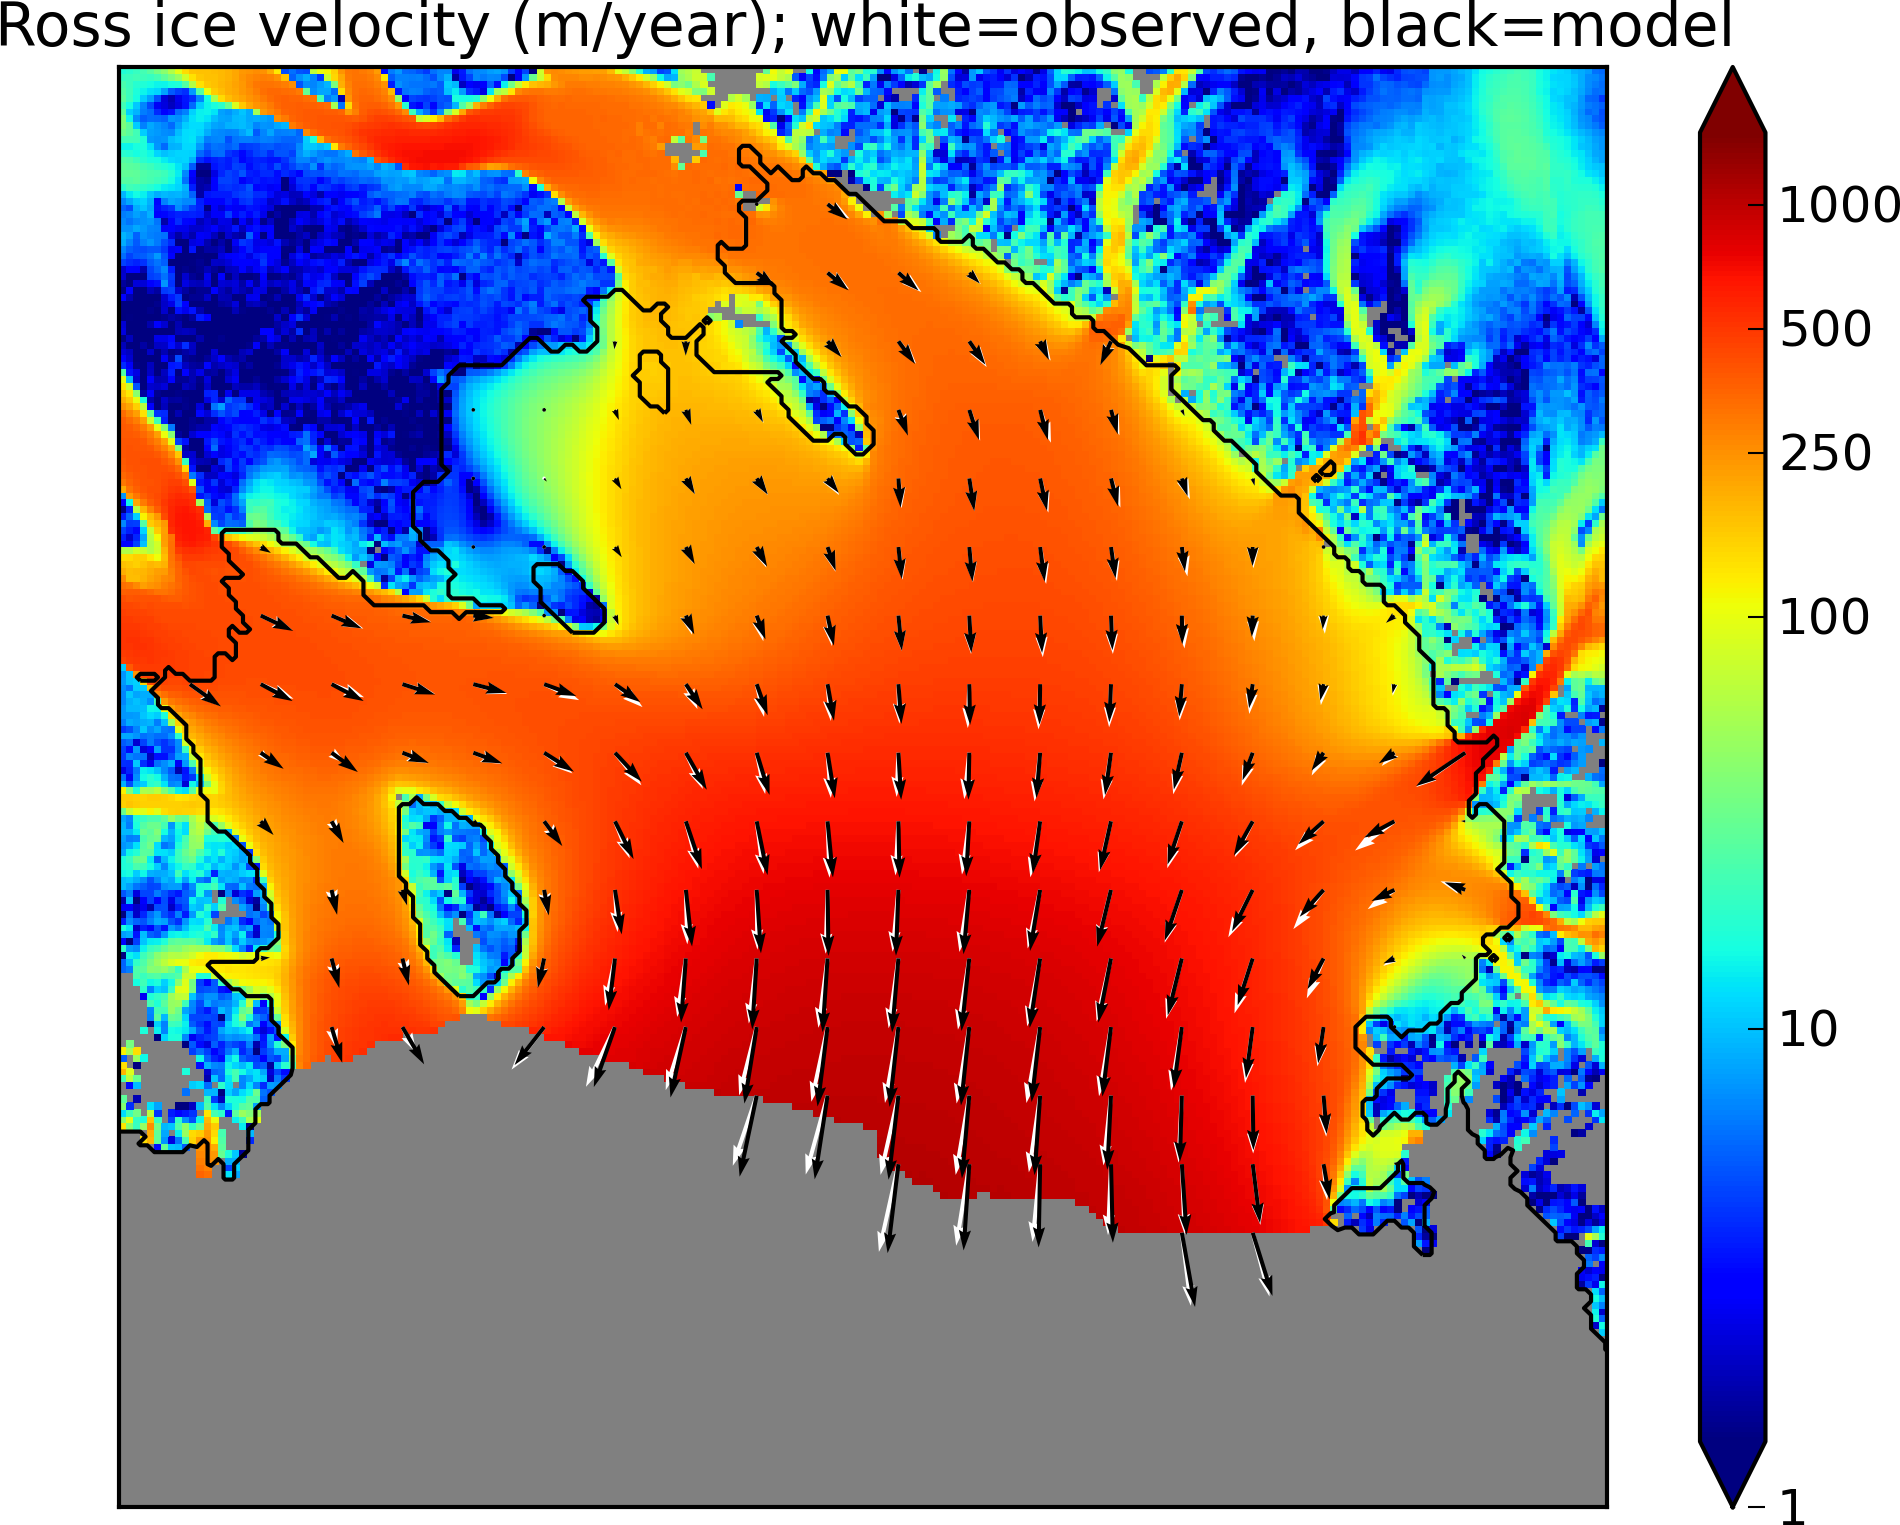
\includegraphics[width=3.5in,keepaspectratio=true]{rossquiver}
\end{center}

\vspace{.4in}

\large
\begin{center}
\framebox{\parbox{5.0in}{ \emph{WARNING}:\index{PISM!warning}  PISM is an ongoing project.  Ice sheet modeling is complicated and is generally not mature.  Please don't trust the results of PISM or any other ice sheet model without a fair amount of exploration.  Also, please don't expect all your questions to be answered here.  Write to us with questions at \href{mailto:help@pism-docs.org}{\texttt{help@pism-docs.org}}.} }
\normalsize
\end{center}
\normalsize


\clearpage\newpage
\section{Getting started}\label{sec:start}\index{PISM!getting started}

This introduction is intended to be interactive and participatory, and it should work on \emph{your personal machine} as well as on a supercomputer.  Please try the commands and view the resulting files.  Do the runs with your own values for the options.  We can't hide the fact that PISM has lots of ``control knobs,'' but fiddling with them will help you get going.  Give it a try!

To install PISM see the \emph{Getting PISM} tab at \href{http://www.pism-docs.org}{\texttt{www.pism-docs.org}}.  Or get the PISM Installation Manual (PDF) at \url{http://www.pism-docs.org/wiki/lib/exe/fetch.php?media=installation.pdf}.  Once PISM is installed, the executable \texttt{pismr} should be available on your system's ``path''; confirm this with ``\texttt{which pismr}''.  The instructions below assume you are using a \texttt{bash} shell or one that accepts \texttt{bash} syntax.  They also assume you have the PISM source code in the directory ``\texttt{pism/}''.

\subsection{A Greenland ice sheet example}

We get started with an extended example showing how to generate initial states for prognostic model experiments on the Greenland ice sheet.  Ice sheet and glacier model studies often involve modeling present and past states using actions like the ones demonstrated here.  Our particular choices made here are motivated by the evaluation of initialization methods in \cite{AschwandenAdalgeirsdottirKhroulev}.

We use data assembled by the \href{http://websrv.cs.umt.edu/isis/index.php/SeaRISE_Assessment}{Sea-level Response to Ice Sheet Evolution (SeaRISE)} assessment process\index{SeaRISE!data} \cite{Bindschadler2013SeaRISE}.  SeaRISE is a community-organized assessment process providing an upper bound on ice sheet contributions to sea level in the next 100--200 years, especially for the IPCC AR5 report in 2013.

This example is a hands-on first look at PISM.  It is not an in-depth tutorial, and some details of what is happening are only explained later in this Manual, which thoroughly discusses PISM options, nontrivial modeling choices, and how to preprocess input data.

The basic runs here, mostly on coarse $20$ and $10\,\textrm{km}$ grids, can be done on a typical workstation or laptop.  PISM is, however, designed to make high resolution (e.g.~$5\,\textrm{km}$ to $1\,\textrm{km}$ grids for whole-Greenland ice sheet modeling) possible by exploiting large-scale parallel processing.  See \cite{AschwandenAdalgeirsdottirKhroulev,Golledgeetal2012,Golledgeetal2013}, among other published high-resolution PISM examples.


\subsection{Input data}

The NetCDF data used to initialize SeaRISE runs is freely-available online: 
\medskip

\centerline{\protect{\textbf{\url{http://websrv.cs.umt.edu/isis/index.php/Present_Day_Greenland}}}}
\medskip

\noindent To download the specific file we want, namely \texttt{Greenland_5km_v1.1.nc}, and preprocess it for PISM, do:
\begin{verbatim}
$ cd pism/examples/std-greenland
$ ./preprocess.sh
\end{verbatim}
\noindent The script \texttt{preprocess.sh} requires \texttt{wget} and also the NetCDF Operators (``NCO''; \url{http://nco.sourceforge.net/}).  It downloads the version 1.1 of the SeaRISE ``master'' present-day data set, which contains ice thickness and bedrock topography from BEDMAP \cite{BamberLayberryGogenini}, and modeled precipitation and surface mass balance rates from RACMO \cite{Ettemaetal2009}, among other fields.

In particular, it creates three new NetCDF files which can be read by PISM.  The spatially-varying fields, with adjusted metadata, go in \texttt{pism_Greenland_5km_v1.1.nc}.  The other two new files contain famous time-dependent paleo-climate records from ice and seabed cores: \texttt{pism_dT.nc} has the GRIP temperature record \cite{JohnsenetalGRIP} and \texttt{pism_dSL.nc} has the SPECMAP sea level record \cite{Imbrieetal1984}.

Any of these NetCDF files can be viewed with \texttt{ncview} or other NetCDF visualization tools; see Table \ref{tab:NetCDFview} below.  An application of IDV to the master data set produced Figure \ref{fig:sr-input}, for example.  Use \texttt{ncdump -h} to see the metadata and history of the files.

\begin{figure}[ht]
\centering
\mbox{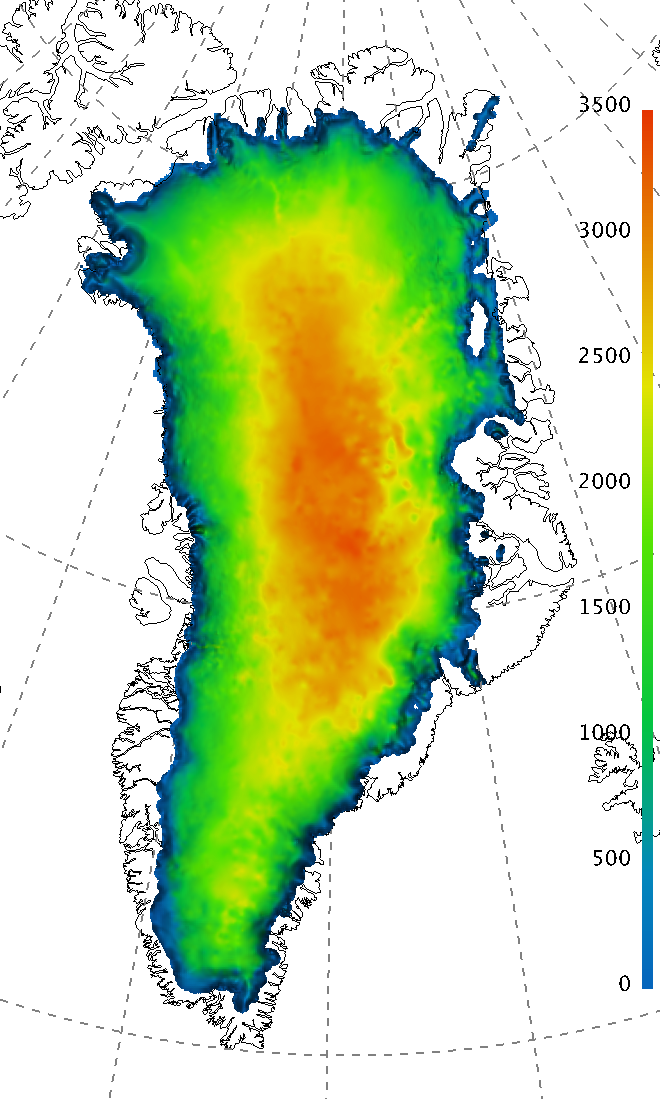
\includegraphics[width=2.0in,keepaspectratio=true]{sr-greenland-thk}
  \qquad
  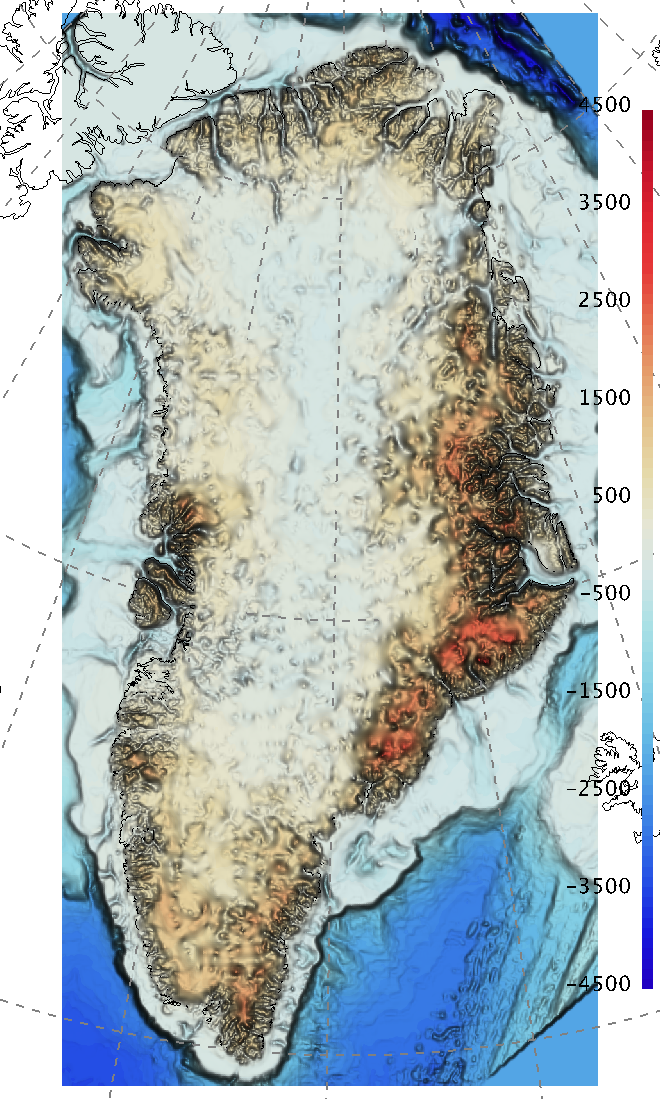
\includegraphics[width=2.0in,keepaspectratio=true]{sr-greenland-topg}
  \qquad
  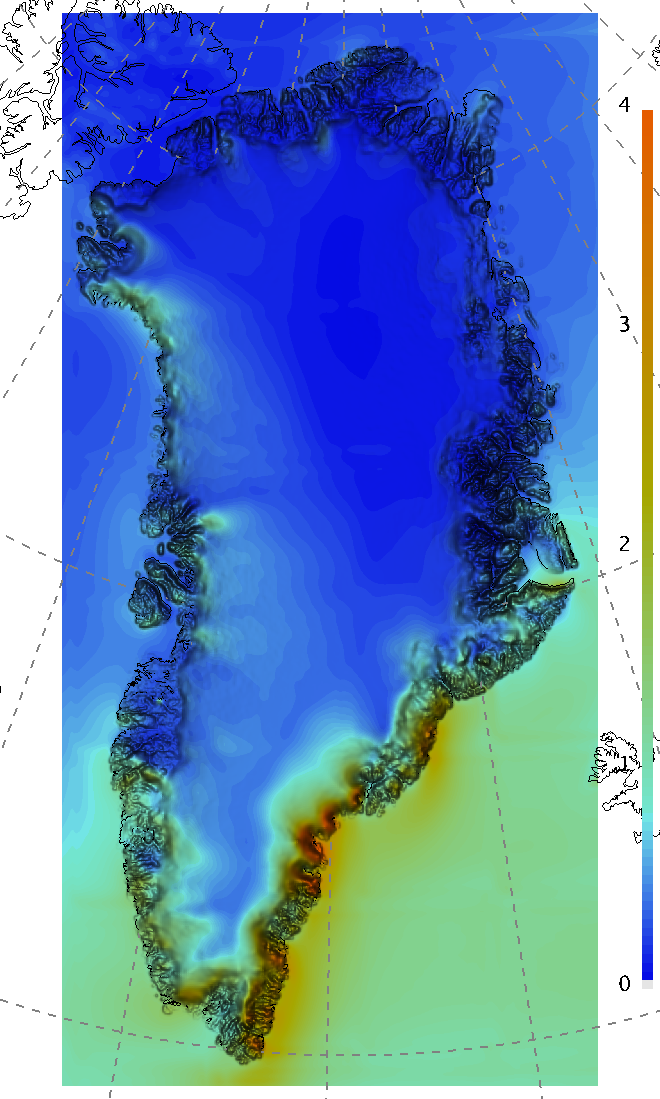
\includegraphics[width=2.0in,keepaspectratio=true]{sr-greenland-prcp}}
\caption{The input file contains present-day ice thickness (left; m), bedrock elevation (center; m), and present-day precipitation (right; m $\text{a}^{-1}$ ice equivalent) for SeaRISE-Greenland.  These are fields \texttt{thk}, \texttt{topg}, and \texttt{precipitation}, respectively, in \texttt{pism_Greenland_5km_v1.1.nc}.}
\label{fig:sr-input}
\end{figure}


\subsection{First run}   \label{subsect:runscript}  Like many Unix programs, PISM allows a lot of command-line options.  In fact, because the variety of allowed ice sheet, shelf, and glacier configurations, and included sub-models, is so large, the list of possible command-line options covers sections \ref{sec:initboot} through \ref{sec:practical-usage} of this manual.  In practice one often builds scripts to run PISM with the correct options, which is what we show here.  The script we use is ``\texttt{spinup.sh}'' in the \texttt{examples/std-greenland/} subdirectory of \texttt{pism/}.

Note that initializing ice sheets, generically called ``spin-up'', can be done by computing approximate steady states with constant boundary data, or, in some cases, by integrating paleo-climatic and long-time-scale information, also applied at the ice sheet boundary, to build a model for the present state of the ice sheet.  Both of these possibilities are illustrated in the \texttt{spinup.sh} script.  The spin-up stage of using an ice sheet model may actually require more processor-hours than follow-on ``experiment'' or ``forecast'' stages.

To see what can be done with the script, read the usage message it produces:
\begin{verbatim}
$ ./spinup.sh
\end{verbatim}

The simplest spin-up approach is to use a ``constant-climate'' model.  We take this approach first.  To see a more detailed view of the PISM command for the first run, do:
\begin{verbatim}
$ PISM_DO=echo ./spinup.sh 4 const 10000 20 sia g20km_10ka.nc
\end{verbatim}
Setting the environment variable \texttt{PISM_DO} in this way tells \texttt{spinup.sh} just to print out the commands it is about to run, not do them.  The ``proposed'' run looks like this:
\label{firstcommand}
\small
\begin{verbatim}
mpiexec -n 4 pismr -boot_file pism_Greenland_5km_v1.1.nc -Mx 76 -My 141 \
  -Mz 101 -Mbz 11 -z_spacing equal -Lz 4000 -Lbz 2000 -skip -skip_max 10 \
  -ys -10000 -ye 0 -surface given -surface_given_file pism_Greenland_5km_v1.1.nc \
  -calving ocean_kill pism_Greenland_5km_v1.1.nc -sia_e 3.0 \
  -ts_file ts_g20km_10ka.nc -ts_times -10000:yearly:0 \
  -extra_file ex_g20km_10ka.nc -extra_times -10000:100:0 \
  -extra_vars diffusivity,temppabase,tempicethk_basal,bmelt,tillwat,csurf,mask,thk,topg,usurf \
  -o g20km_10ka.nc
\end{verbatim}
\normalsize
Let's briefly deconstruct this run.

At the front is ``\texttt{mpiexec -n 4 pismr}''.  This means that the PISM executable \texttt{pismr} is run in parallel on four processes parallel standard (e.g.~cores) under the Message Passing Interface (``MPI''; \url{http://www.mcs.anl.gov/mpi/}).  Though we are assuming you have a workstation or laptop with at least 4 cores, this example will work with 1 to about 50 processors, with reasonably good scaling in speed.  Scaling can be good with more processors if we run at higher spatial resolution \cite{BBssasliding,DickensMorey2013}.  The executable name ``\texttt{pismr}'' stands for the standard ``run'' mode of PISM (in contrast to specialized modes described later in sections \ref{sec:verif} and \ref{sec:simp}).

Next, the proposed run uses option \texttt{-boot_file} to start the run by ``bootstrapping.'' This term describes the creation, by heuristics and highly-simplified models, of the mathematical initial conditions required for a deterministic, time-dependent ice dynamics model.  Then the options describe a $76\times 141$ point grid in the horizontal, which gives 20 km grid spacing in both directions.  Then there are choices about the vertical extent and resolution of the computational grid; more on those later.  After that we see a description of the time-axis, with a start and end time given: ``\texttt{-ys -10000 -ye 0}''.

Then we get the instructions that tell PISM to read the upper surface boundary conditions (i.e.~climate) from a file: ``\texttt{-surface given -surface_given_file pism_Greenland_5km_v1.1.nc}''.  For more on these choices, see subsection \ref{sec:climate-inputs}, and also the PISM Climate Forcing Manual.

Then there are a couple of options related to ice dynamics.  First is a minimal calving model which removes ice at the calving front location given by a thickness field in the input file (``\texttt{-calving ocean_kill}''); see subsection \ref{sec:calving} for this and other calving options).  Then there is a setting for enhanced ice softness (``\texttt{-sia_e 3.0}'').  See subsection \ref{sec:rheology} for more on this enhancement parameter, which we also return to later in the current section in a parameter study.

Then there are longish options describing the fields we want as output, including scalar time series (``\texttt{-ts_file ts_g20km_10ka.nc -ts_times -10000:yearly:0}''; see section \ref{sec:practical-usage}) and space-dependent fields (``\texttt{-extra_file ...}''; again see section \ref{sec:practical-usage}), and finally the named output file (``\texttt{-o g20km_10ka.nc}'').

Note that the modeling choices here are reasonable, but they are not the only way to do it! The user is encouraged to experiment; that is the point of a model.

Now let's actually get the run going:
\begin{verbatim}
$ ./spinup.sh 4 const 10000 20 sia g20km_10ka.nc &> out.g20km_10ka &
\end{verbatim}
\noindent The terminating ``\verb|&|'' asks unix to run the command in the background, so we can keep working in the current shell.  Because we have re-directed the text output (``\verb|&> out.g20km_10ka|''), PISM will show what it is doing in the text file \texttt{out.g20km_10ka}.  Using \texttt{less} is a good way to watch such a growing text-output file.  This run should take only 20 minutes or so.


\subsection{Watching the first run}  \label{subsect:watchrun}  As soon as the run starts it creates time-dependent NetCDF files \texttt{ts_g20km_10ka.nc} and \texttt{ex_g20km_10ka.nc}.  The latter file, which has spatially-dependent fields at each time, is created after the first 100 model years, a few wall clock seconds in this case.  The command \texttt{-extra_file ex_g20km_10ka.nc -extra_times -10000:100:0} adds a spatially-dependent ``frame'' at model times -9900, -9800, \dots, 0.

To look at the spatial-fields output graphically, do:
\begin{verbatim}
$ ncview ex_g20km_10ka.nc
\end{verbatim}
We see that \texttt{ex_g20km_10ka.nc} contains growing ``movies'' of the fields chosen by the \texttt{-extra_vars} option.  A frame of the ice thickness field \texttt{thk} is shown in Figure \ref{fig:growing} (left).

The time-series file \texttt{ts_g20km_10ka.nc} is also growing.  It contains spatially-averaged ``scalar'' diagnostics like the total ice volume or the ice-sheet-wide maximum velocity (variable \texttt{ivol} and \texttt{max_hor_vel}, respectively).  It can be viewed
\begin{verbatim}
$ ncview ts_g20km_10ka.nc
\end{verbatim}
The growing time series for \texttt{ivol} is shown in Figure \ref{fig:growing} (right).  Recall that our intention was to generate a minimal model of the Greenland ice sheet in approximate steady-state with a steady (constant-in-time) climate.  The measurable steadiness of the \texttt{ivol} time series is a possible standard for steady state \cite[for example]{EISMINT00}.

\begin{figure}[ht]
\centering
\mbox{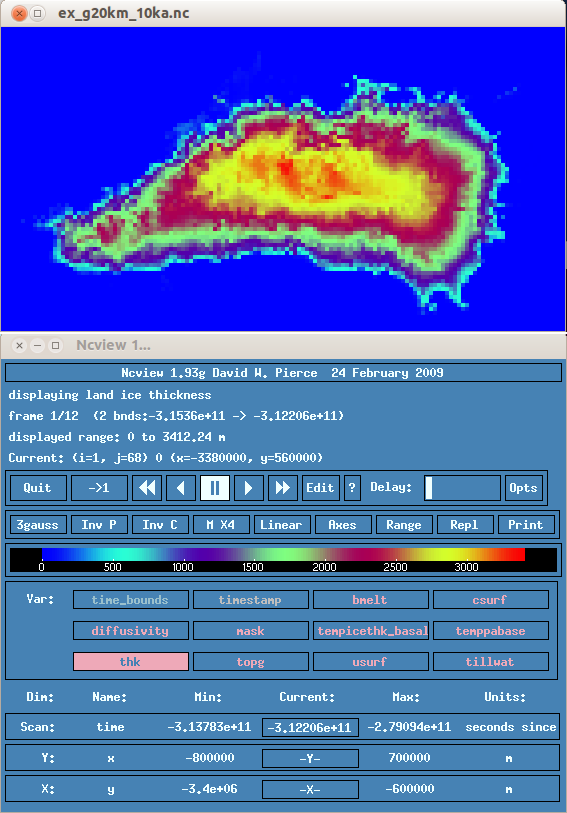
\includegraphics[height=5.0in,keepaspectratio=true]{ex-growing-thk-g20km}
  \qquad 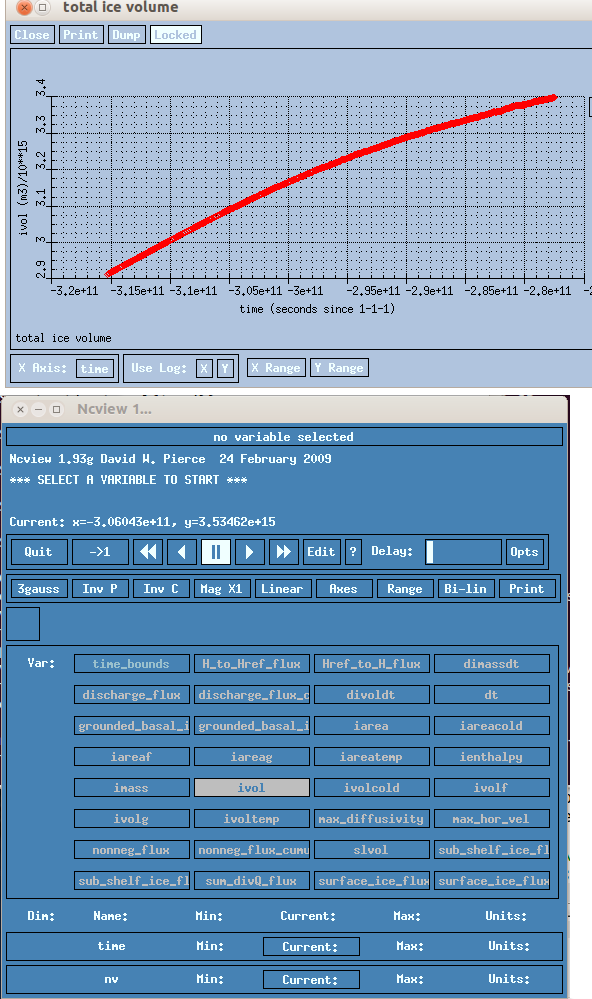
\includegraphics[height=5.0in,keepaspectratio=true]{ts-growing-ivol-g20km}}
\caption{Two views produced by \texttt{ncview} during a PISM model run.  Left: \texttt{thk}, the ice sheet thickness, a space-dependent field, from file \texttt{ex_g20km_10ka.nc}.  Right: \texttt{ivol}, the total ice sheet volume time-series, from file \texttt{ts_g20km_10ka.nc}.}
\label{fig:growing}
\end{figure}

At the end of the run the output file \texttt{g20km_10ka.nc} is generated.  Figure \ref{fig:firstoutput} shows some fields from this file.  In the next subsections we consider their ``quality'' as model results.  To see a report on computational performance, we do:
\begin{verbatim}
$ ncdump -h g20km_10ka.nc |grep history
    :history = "user@machine 2013-11-23 15:57:22 AKST: PISM done.  Performance stats:
0.3435 wall clock hours, 1.3738 proc.-hours, 7274.0065 model years per proc.-hour,
PETSc MFlops = 0.03.\n",
\end{verbatim}

\begin{figure}[ht]
\centering
\mbox{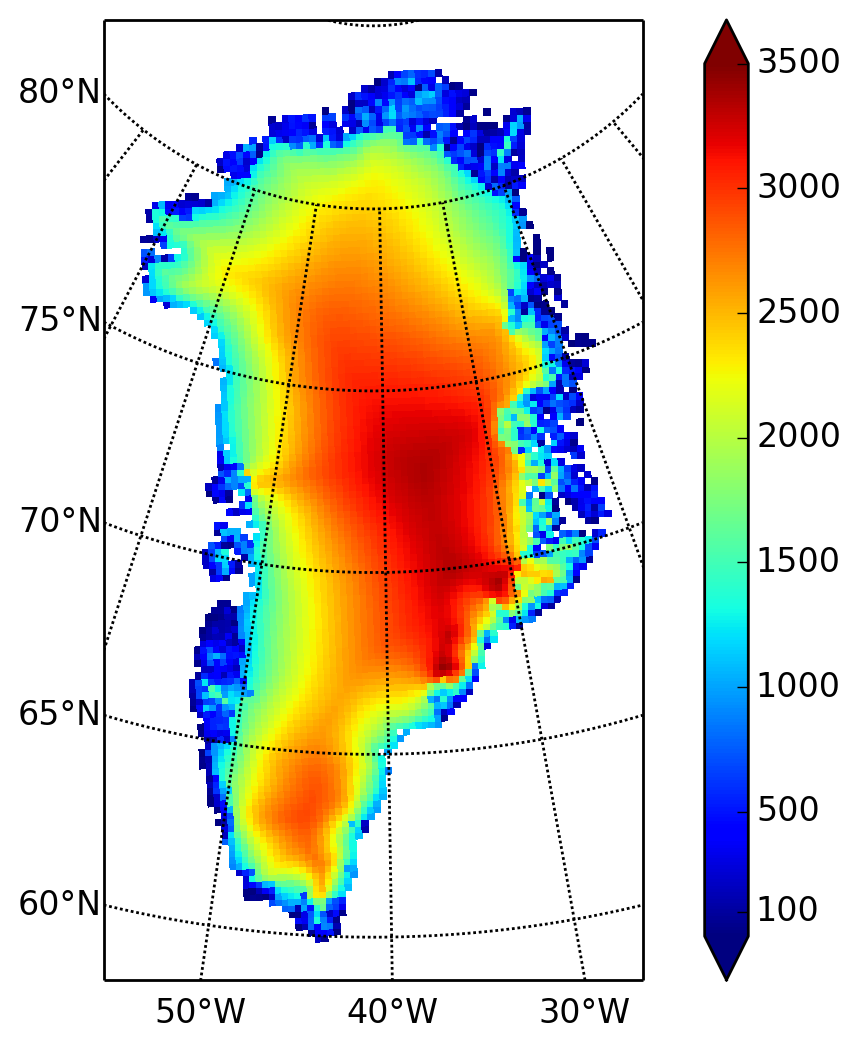
\includegraphics[height=2.75in,keepaspectratio=true]{g20km-10ka-usurf} 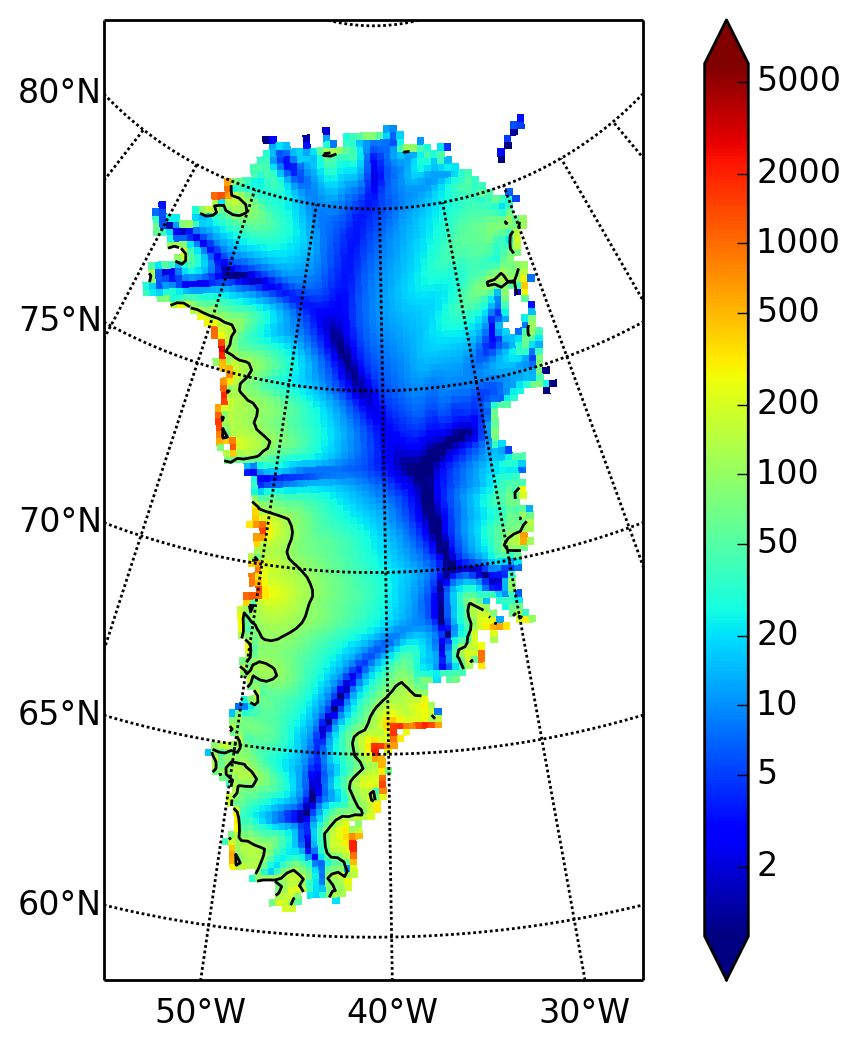
\includegraphics[height=2.75in,keepaspectratio=true]{g20km-10ka-csurf} 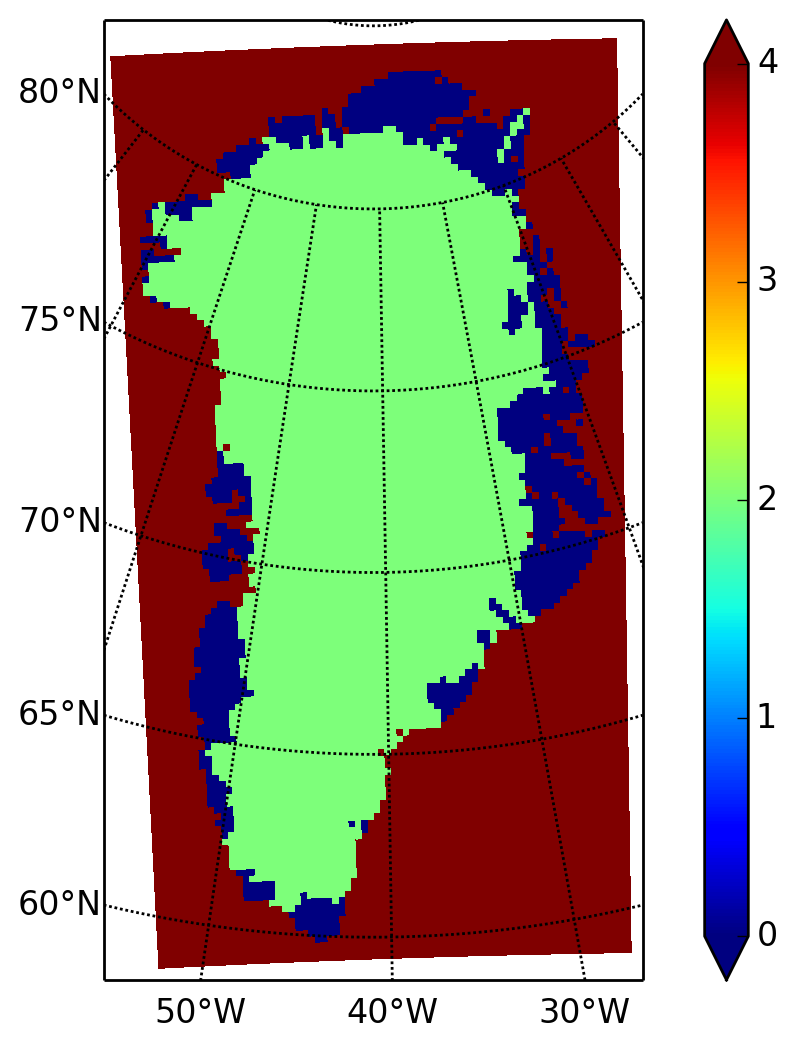
\includegraphics[height=2.75in,keepaspectratio=true]{g20km-10ka-mask}}
\caption{Fields from output file \texttt{g20km_10ka.nc}.  Left: \texttt{usurf}, the ice sheet surface elevation in meters.  Middle: \texttt{csurf}, the surface speed in meters/year ($=$ m/a), including the 100 m/a contour (solid black).  Right: \texttt{mask}, with 0 = ice-free land, 2 = grounded ice, 4 = ice-free ocean.}
\label{fig:firstoutput}
\end{figure}


\subsection{Second run: a better ice-dynamics model}  \label{subsect:ssarun}

It is widely-understood that ice sheets slide on their bases, especially when liquid water is present at the base (see \cite{Joughinetal2001,MacAyeal}, among others).  An important aspect of modeling such sliding is the inclusion of membrane or ``longitudinal'' stresses into the stress balance \cite{BBssasliding}.  The basic stress balance in PISM which involves membrane stresses is the Shallow Shelf Approximation (SSA) \cite{WeisGreveHutter}.  The stress balance used in the previous section was, by contrast, the (thermomechanically-coupled) non-sliding, non-membrane-stress Shallow Ice Approximation (SIA) \cite{BBL,EISMINT00}.  The preferred ice dynamics model within PISM, that allows both sliding balanced by membrane stresses and shear flow as described by the SIA, is the SIA+SSA ``hybrid'' model \cite{BBssasliding,Winkelmannetal2011}.  For more on stress balance theories see section \ref{sec:dynamics} of this Manual.

The practical issue with models of sliding is that a distinctly-uncertain parameter space must be introduced.  This especially involves parameters controlling the amount and pressure of subglacial water (see \cite{AschwandenAdalgeirsdottirKhroulev,Clarke05,Tulaczyketal2000,vanPeltOerlemans2012} among other references).  In this regard, PISM uses the concept of a saturated and pressurized subglacial till with a modeled distribution of yield stress  \cite{BBssasliding,SchoofStream}.  The yield stress arises from the PISM model of the production of subglacial water, which is itself computed through the conservation of energy model \cite{AschwandenBuelerKhroulevBlatter}.  We use such models in the rest of this Getting Started section.

While the \texttt{spinup.sh} script has default sliding-related parameters, for demonstration purposes we change one parameter.  We replace the default power $q=0.25$ in the sliding law (the equation which relates both the subglacial sliding velocity and the till yield stress to the basal shear stress which appears in the SSA stress balance) by a less ``plastic'' and more ``linear'' choice $q=0.5$.  See subsection \ref{subsect:basestrength} for more on sliding laws.  To see the run we propose, do
\begin{verbatim}
$ PISM_DO=echo PARAM_PPQ=0.5 ./spinup.sh 4 const 10000 20 hybrid g20km_10ka_hy.nc
\end{verbatim}
Now remove ``\texttt{PISM_DO=echo}'' and redirect the text output into a file to start the run:
\begin{verbatim}
$ PARAM_PPQ=0.5 ./spinup.sh 4 const 10000 20 hybrid g20km_10ka_hy.nc &> out.g20km_10ka_hy &
\end{verbatim}
This run might take 30 minutes or so.\footnote{Regarding the relative speeds of the runs that produce \texttt{g20km_10ka.nc} and \texttt{g20km_10ka_hy.nc}, note that the computation of the SSA stress balance is substantially more expensive than the SIA in a per-step sense.  However, the SSA stress balance in combination with the mass continuity equation causes the maximum diffusivity in the ice sheet to be substantially lower during the run.  Because the maximum diffusivity controls the time-step in the PISM adaptive time-stepping scheme \cite{BBL}, the number of time steps is reduced in the hybrid run.  To see this contrast do\, \texttt{ncview ts_g20km_10ka*nc}\, and view variables \texttt{max_diffusivity} and \texttt{dt}. }

When this run is finished it produces \texttt{g20km_10ka_hy.nc}.  As before do
\begin{verbatim}
$ ncdump -h g20km_10ka_hy.nc |grep history
\end{verbatim}
to see performance results for your machine.  The number reported as ``\texttt{PETSc MFlops}'' from this run is about $2.6 \times 10^5$, much larger than the previous run, because now calls to the PETSc library are used when solving the non-linear and non-local SSA stress balance in parallel.

The results of this run are shown in Figure \ref{fig:secondoutputcoarse}.  We show the basal sliding speed field \texttt{cbase} in this Figure, where Figure \ref{fig:firstoutput} had the \texttt{mask}, but the reader can check that \texttt{cbase}=0 in the nonsliding SIA-only result \texttt{g20km_10ka.nc}.

\begin{figure}[ht]
\centering
\mbox{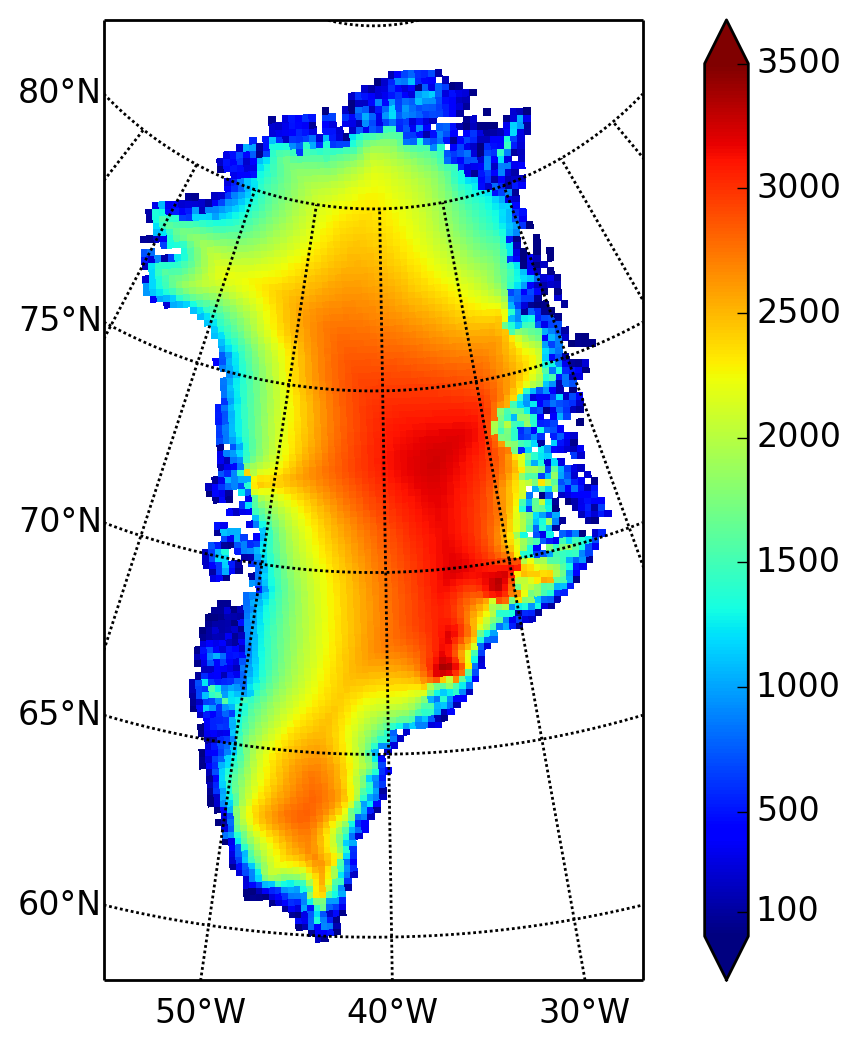
\includegraphics[height=2.75in,keepaspectratio=true]{g20km-10ka-hy-usurf} 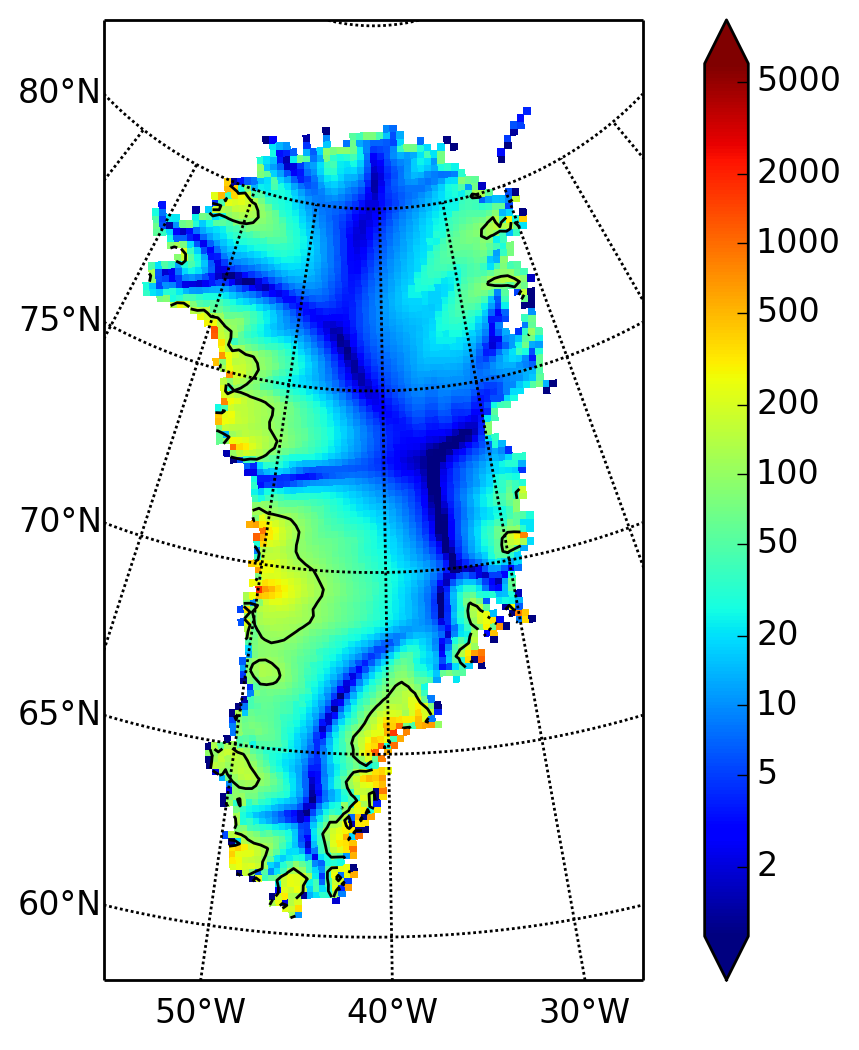
\includegraphics[height=2.75in,keepaspectratio=true]{g20km-10ka-hy-csurf} 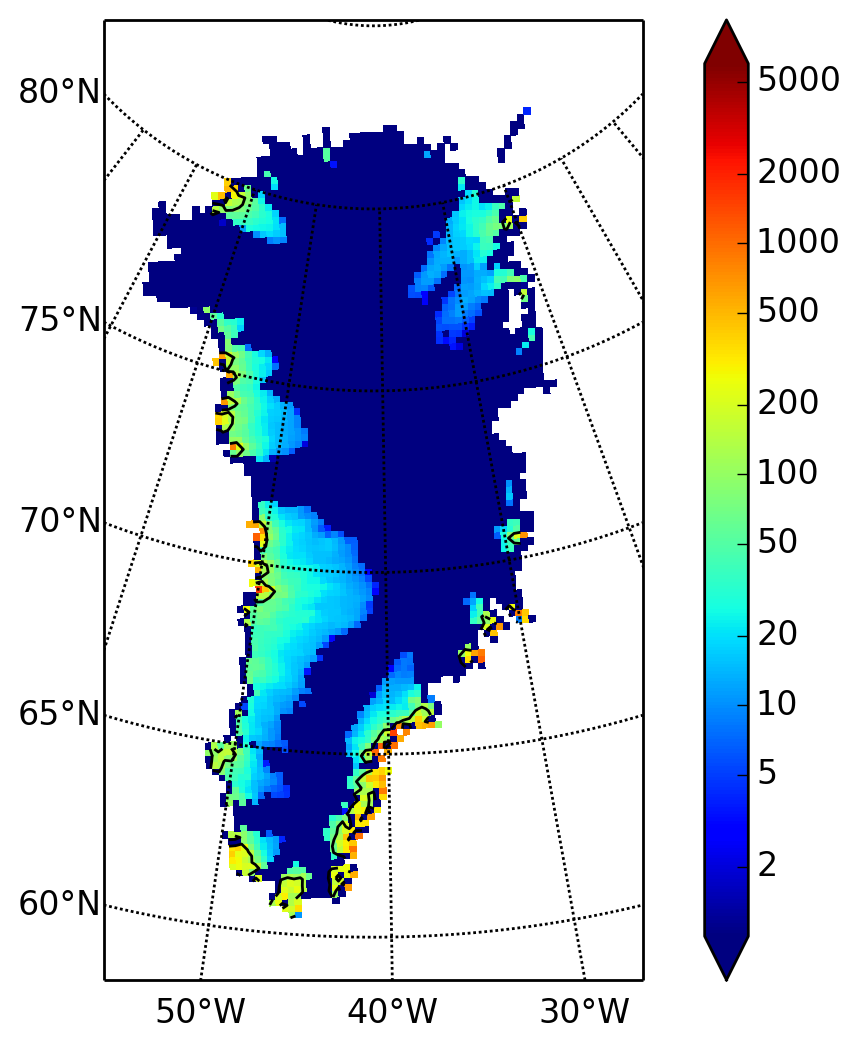
\includegraphics[height=2.75in,keepaspectratio=true]{g20km-10ka-hy-cbase}}
\caption{Fields from output file \texttt{g20km_10ka_hy.nc}.  Left: \texttt{usurf}, the ice sheet surface elevation in meters.  Middle: \texttt{csurf}, the surface speed in m/a, including the 100 m/a contour (solid black).  Right: the sliding speed \texttt{cbase}, shown the same way as \texttt{csurf}.}
\label{fig:secondoutputcoarse}
\end{figure}

The hybrid model includes sliding, and it is important to evaluate that aspect of the output.  However, though it is critical to the response of the ice to changes in climate, basal sliding velocity is essentially unobservable in real ice sheets.  On the other hand, because of relatively-recent advances in radar and image technology and processing \cite{Joughin2002}, the surface velocity of an ice sheet is an observable.  So, how good is our model result for this quantity, namely \texttt{csurf}?  Figure \ref{fig:csurfvsobserved} compares the radar-observed \texttt{surfvelmag} field in the downloaded SeaRISE-Greenland data file \texttt{Greenland_5km_v1.1.nc} with the just-computed PISM result.

\begin{figure}[ht]
\centering
\mbox{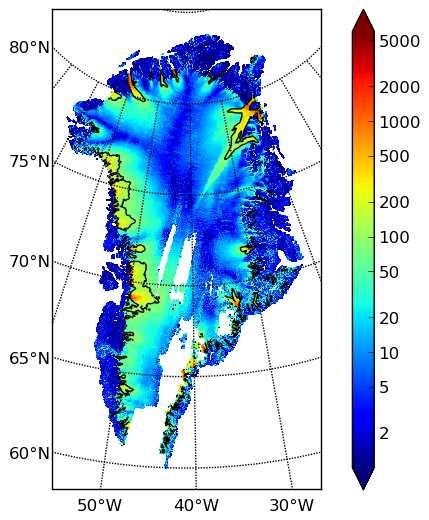
\includegraphics[height=2.75in,keepaspectratio=true]{Greenland-5km-v1p1-surfvelmag} 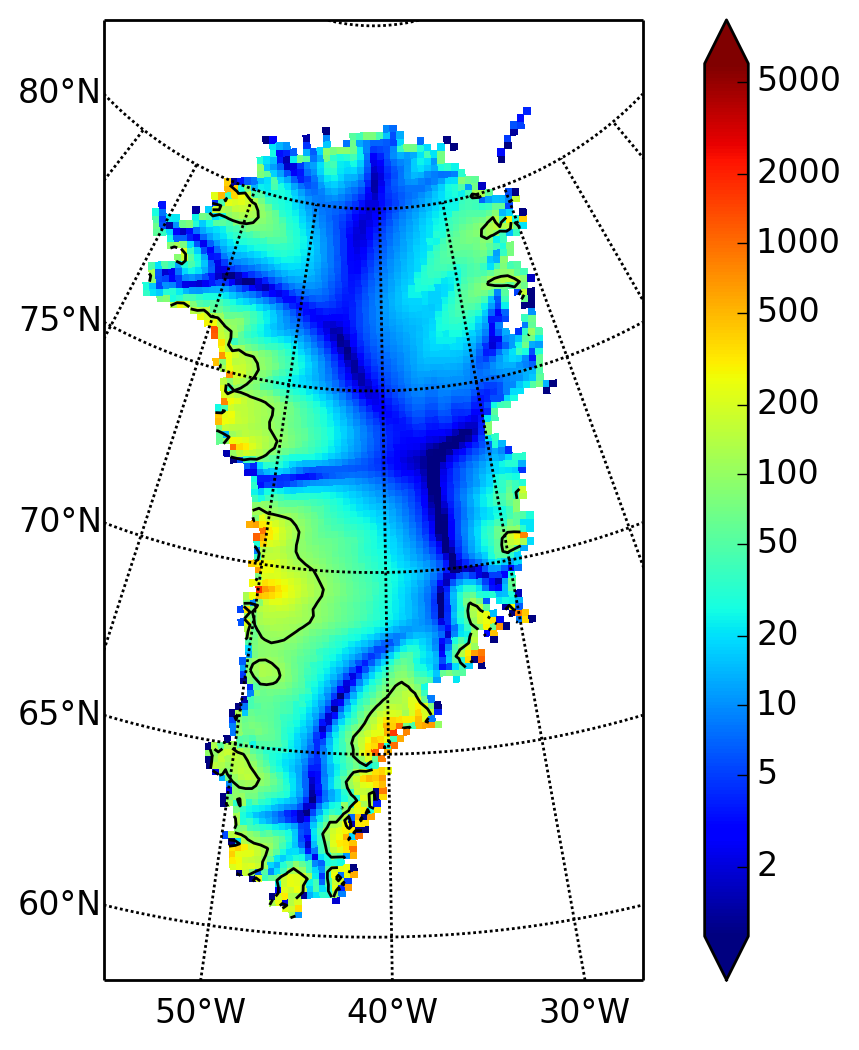
\includegraphics[height=2.75in,keepaspectratio=true]{g20km-10ka-hy-csurf} 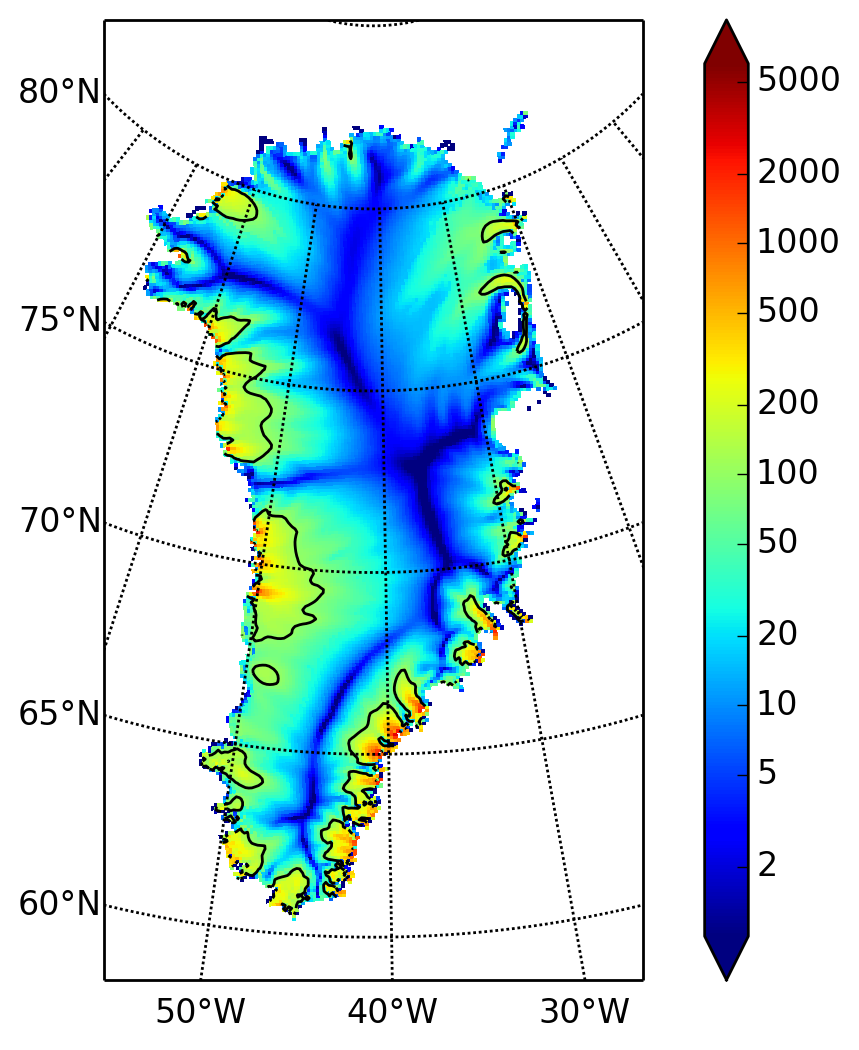
\includegraphics[height=2.75in,keepaspectratio=true]{g10km-10ka-hy-csurf}}
\caption{Comparing observed and modeled surface speed.  All figures have a common scale (m/a), with 100 m/a contour shown (solid black).  Left: \texttt{surfvelmag}, the observed values from SeaRISE data file \texttt{Greenland_5km_v1.1.nc}.  Middle: \texttt{csurf} from \texttt{g20km_10ka_hy.nc}.  Right: \texttt{csurf} from \texttt{g10km_10ka_hy.nc}.}
\label{fig:csurfvsobserved}
\end{figure}

The reader might agree with these broad qualitative judgements:
\begin{itemize}
\item the model results and the observed surface velocity look similar, but
\item the slow flow near the divide is generally in the right areas and of generally the right magnitude, and
\item the observed Northeast Greenland ice stream is much more distinct in observations than in the model.
\end{itemize}

We can compare these easily-generated PISM results to some recent observed-vs-model comparisons of surface velocity maps, of exactly this type, for example Figure 1 in \cite{Priceetal2011} and Figure 8 in \cite{Larouretal2012}.  Note that only ice-sheet-wide parameters and models were used here in PISM, that is, each location in the ice sheet was modeled by the same physics.  By comparison, those published comparisons involved tuning a large number of subglacial parameters to values which would yield close match to observations of the surface velocity.  Such tuning techniques are usually called ``inversion'' or ``assimilation'' of the surface velocity data.  Such methods are also possible in PISM if desired,\footnote{See \cite{vanPeltetal2013} (inversion of DEMs for basal topography) and \cite{Habermannetal2013} (inversion surface velocities for basal shear stress) for PISM-based inversion methods and analysis.} but the advantage of having few parameters in a model is well-known: the results reflect the underlying model not the flexibility of fitting many parameters.

Of course, we have only tried two of the many models possible in PISM.  We are free to identify and adjust important parameters.  The first parameter change we consider, in the next subsection, is one of the most important: grid resolution.


\subsection{Third run: higher resolution}  \label{subsect:higherresrun}

Now we change one key parameter, the grid resolution.  If you can let it run overnight, do
\begin{verbatim}
$ PARAM_PPQ=0.5 ./spinup.sh 4 const 10000 10 hybrid g10km_10ka_hy.nc &> out.g10km_10ka_hy &
\end{verbatim}
This run might take 4 to 6 hours.  However, supposing you have a larger parallel computer, you can change ``\texttt{mpiexec -n 4}'' to ``\texttt{mpiexec -n N}'' where \texttt{N} is a substantially larger number, up to 100 or so with an expectation of reasonable scaling on this grid \cite{BBssasliding,DickensMorey2013}.

Some fields from the result \verb|g10km_10ka_hy.nc| are shown in Figure \ref{fig:secondoutputfiner}.  Figure \ref{fig:csurfvsobserved} also compares observed velocity to the model results from 20 km and 10 km grids.  Model results differ even when the only change is the resolution!  Importantly for ice sheet modeling, using higher resolution ``picks up'' more detail in the bed elevation and climate data.

\begin{figure}[ht]
\centering
\mbox{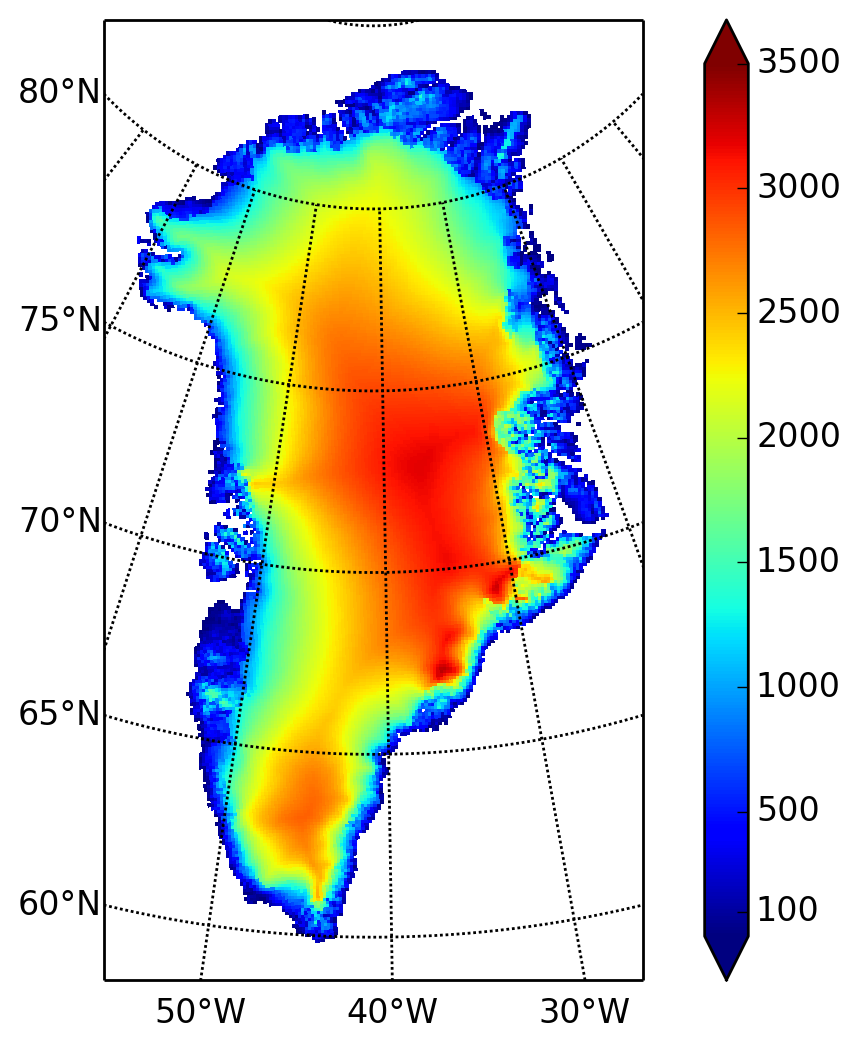
\includegraphics[height=2.75in,keepaspectratio=true]{g10km-10ka-hy-usurf} 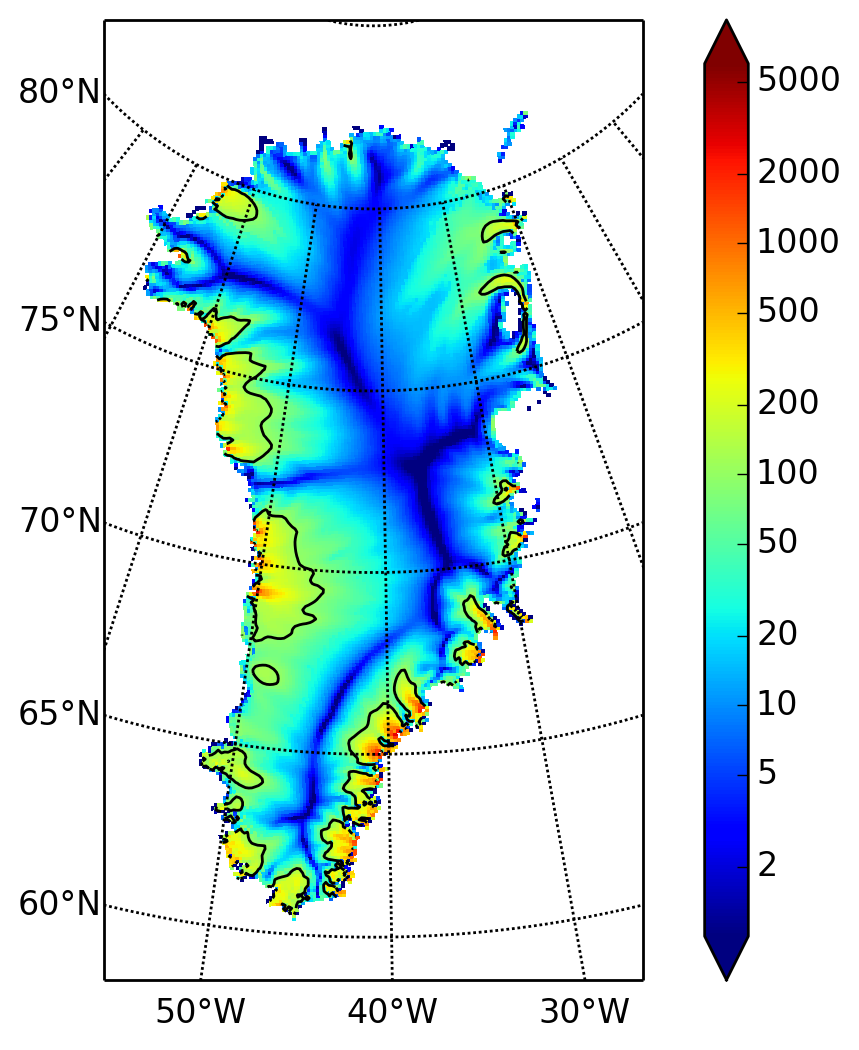
\includegraphics[height=2.75in,keepaspectratio=true]{g10km-10ka-hy-csurf} 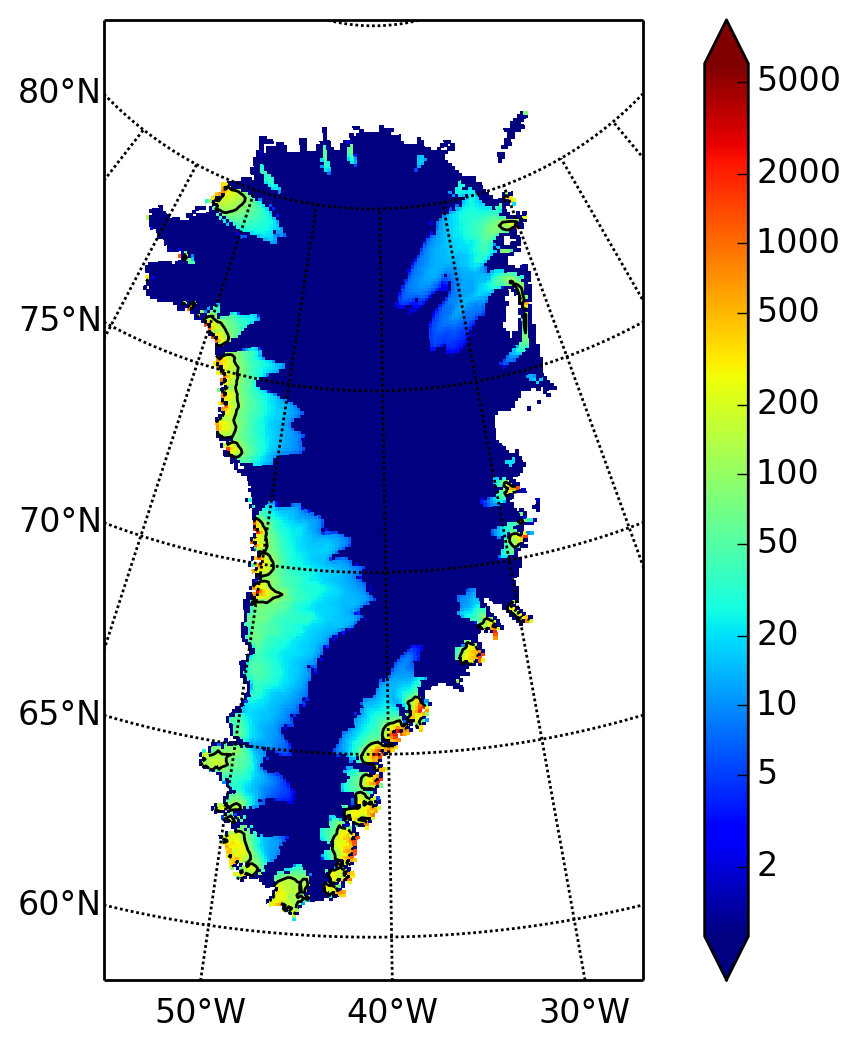
\includegraphics[height=2.75in,keepaspectratio=true]{g10km-10ka-hy-cbase}}
\caption{Fields from output file \texttt{g10km_10ka_hy.nc}.  Compare Figure \ref{fig:secondoutputcoarse}, which only differs by resolution.  Left: \texttt{usurf} in meters.  Middle: \texttt{csurf} in m/a.  Right: \texttt{cbase} in m/a.}
\label{fig:secondoutputfiner}
\end{figure}

As a different kind of comparison, Figure \ref{fig:ivolboth} shows ice volume time series \texttt{ivol} for 20km and 10km runs done here.  We see that this result depends on resolution, in particular because higher resolution grids allow the model to better resolve the flux through topographically-controlled outlet glaciers (compare \cite{Pfefferetal2008}).  However, because the total ice sheet volume is a highly-averaged quantity, the \texttt{ivol} difference from 20km and 10km resolution runs is only about one part in 60 (about 1.5\%) at the final time.  By contrast, as is seen in the near-margin ice in various locations shown in Figure \ref{fig:csurfvsobserved}, the ice velocity at a particular location may change by 100\% when the resolution changes from 20km to 10km.

Roughly speaking, the reader should only consider trusting those model results which are demonstrated to be robust across a range of model parameters, and, in particular, which are shown to be relatively-stable among relatively-high resolution results for a particular case.  Using a supercomputer is justified merely to confirm that lower-resolution runs were already ``getting'' a given feature!

\begin{figure}[ht]
\centering
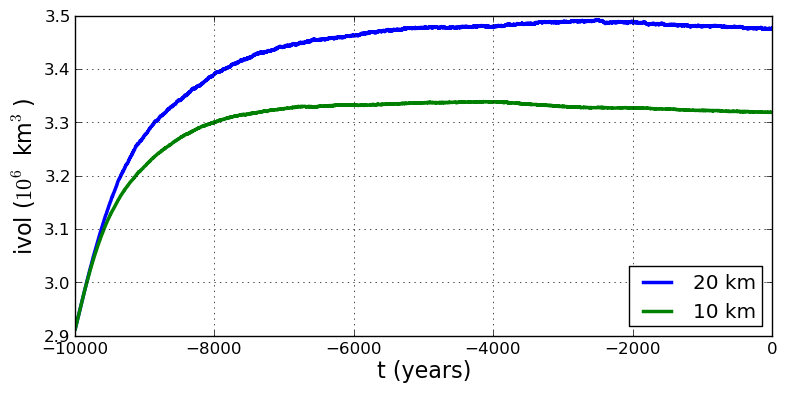
\includegraphics[width=4.0in,keepaspectratio=true]{ivol-both-g20km-g10km}
\caption{Time series of modeled ice sheet volume \texttt{ivol} on 20km and 10km grids.  The present-day ice sheet has volume about $2.9\times 10^6\,\text{km}^3$ \cite{BamberLayberryGogenini}, the initial value seen in both runs.}
\label{fig:ivolboth}
\end{figure}


\subsection{Fourth run: paleo-climate model spin-up}  \label{subsect:paleorun}  

A this point we have barely mentioned one of the most important players in the ice sheet modeling game: the surface mass balance (SMB) model.  Specifically, an SMB model combines precipitation (e.g.~\cite{Balesetal2001} for present-day Greenland) and a model for melt.  Melt models are always based on some approximation of the energy available at the ice surface \cite{Hock05}.  Previous runs in this section used a ``constant-climate'' assumption, which specifically meant using the modeled present-day SMB rates from the regional climate model RACMO \cite{Ettemaetal2009}, as contained in the SeaRISE-Greenland data set \verb|Greenland_5km_v1.1.nc|.

While a physical model of ice dynamics only describes the movement of the ice, the SMB (and the sub-shelf melt rate) are key inputs which directly determine changes in the boundary geometry.  Boundary geometry changes then feedback to determine the stresses seen by the stress balance and thus the motion.

There are other methods for producing SMB than to use present-day modeled values.  We now try such a method, a ``paleo-climate spin-up'' for our Greenland ice sheet model.  Of course, direct measurements of prior climates in Greenland are not available as data!  There are, however, estimates of past surface temperatures at the locations of ice cores \cite[for GRIP]{JohnsenetalGRIP}, along with estimates of past global sea level \cite{Imbrieetal1984} which can be used to determine where the flotation criterion is applied---this is how PISM's \verb|mask| variable is determined.  Also, models have been constructed for how precipitation differs from the present-day values \cite{Huybrechts02}.  For demonstration purposes, these are all used in the next run.  The relevant options are further documented in PISM's Climate Forcing Manual.

As noted, one must compute melt in order to compute SMB.  This is done using a temperature-index, ``positive degree-day'' (PDD) model \cite{Hock05}.  Such a PDD model has parameters for how much snow and/or ice is melted when surface temperatures spend time near or above zero degrees.  Again, see the PISM Climate Forcing Manual for relevant options.

To summarize the paleo-climate model applied here, temperature offsets from the GRIP core record affect the snow energy balance, and thus the rates of melting and runoff calculated by the PDD model.  In warm periods there is more marginal ablation, but precipitation may also increase (according to a temperature-offset model \cite{Huybrechts02}).  Additionally sea level undergoes changes in time and this affects which ice is floating.  Finally we add an earth deformation model, which responds to changes in ice load by changing the bedrock elevation \cite{BLKfastearth}.

To see how all this translates into PISM options, do
\begin{verbatim}
$ PISM_DO=echo PARAM_PPQ=0.5 REGRIDFILE=g20km_10ka_hy.nc \
  ./spinup.sh 4 paleo 25000 20 hybrid g20km_25ka_paleo.nc
\end{verbatim}

\begin{figure}[ht]
\centering
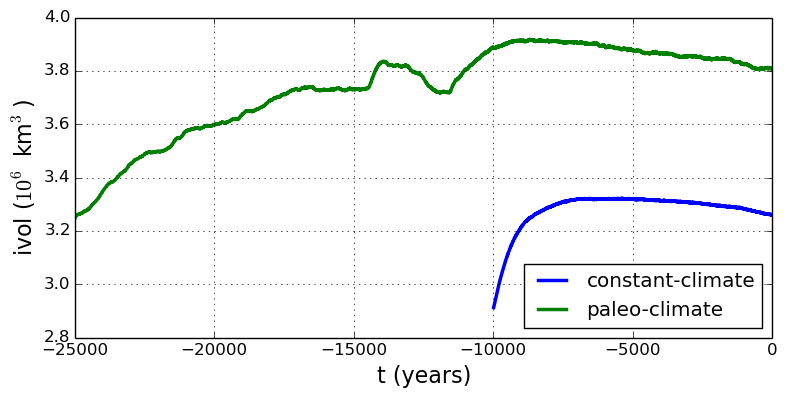
\includegraphics[width=4.5in,keepaspectratio=true]{ivol-const-paleo}
\caption{Time series of modeled ice sheet volume \texttt{ivol} from constant-climate (blue; \texttt{ts_g20km_10ka_hy.nc}) and paleo-climate (red; \texttt{ts_g20km_25ka_paleo.nc}) spinup runs.  Note that the paleo-climate run started with the ice geometry at the end of the constant-climate run.}
\label{fig:ivolconstpaleo}
\end{figure}

You will see an impressive command, which you can compare to the one on page \pageref{firstcommand}.  There are several key changes.  First, we do not start from scratch but instead from a previously computed near-equilibrium result:
\begin{verbatim}
  -regrid_file g20km_10ka_hy.nc -regrid_vars litho_temp,thk,enthalpy,tillwat,bmelt
\end{verbatim}
For more on regridding see subsection \ref{sec:regridding}.  Then we turn on the earth deformation model with option \verb|-bed_def lc|; see subsection \ref{subsect:beddef}.  After that the atmosphere and surface (PDD) models are turned on and the files they need are identified:
\begin{verbatim}
  -atmosphere searise_greenland,delta_T,paleo_precip -surface pdd \
  -atmosphere_paleo_precip_file pism_dT.nc -atmosphere_delta_T_file pism_dT.nc
\end{verbatim}
Then the ocean model, which provides both a subshelf melt rate and a time-dependent sealevel to the ice dynamics core, is turned on with \verb|-ocean constant,delta_SL| and the file it needs is identified with \verb|-ocean_delta_SL_file pism_dSL.nc|.  For all of these ``forcing'' options, see the PISM Climate Forcing Manual.  The remainder of the options are similar or identical to the run that created \verb|g20km_10ka_hy.nc|.

To actually start the run, which we rather arbitrarily start at year -25000, essentially at the LGM, do:
\begin{verbatim}
$ PARAM_PPQ=0.5 REGRIDFILE=g20km_10ka_hy.nc \
  ./spinup.sh 4 paleo 25000 20 hybrid g20km_25ka_paleo.nc &> out.g20km_25ka_paleo &
\end{verbatim}
This run should only take one or two hours, noting it is at a coarse 20 km resolution.

The fields \texttt{usurf}, \texttt{csurf}, and \texttt{cbase} from file \texttt{g20km_25ka_paleo.nc} are sufficiently similar to those shown in Figure \ref{fig:secondoutputcoarse} that they are not shown here.  Close inspection reveals differences, but of course these runs only differ in the applied climate and run duration and not in resolution or ice dynamics parameters.

\begin{figure}[ht]
\centering
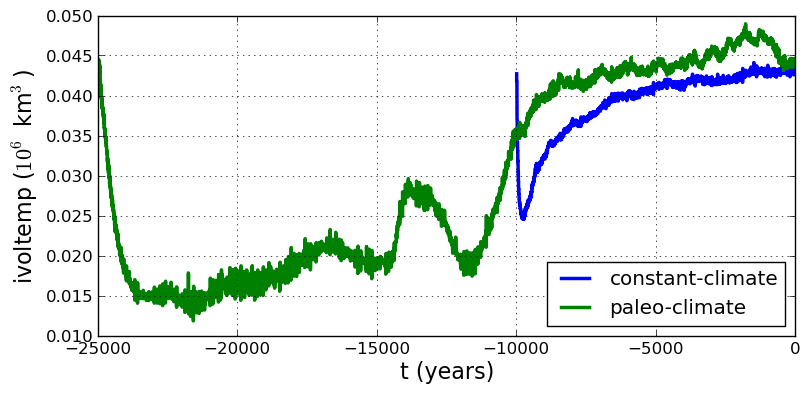
\includegraphics[width=4.5in,keepaspectratio=true]{ivoltemp-const-paleo}
\caption{Time series of temperate ice volume \texttt{ivoltemp} from constant-climate (blue; \texttt{ts_g20km_10ka_hy.nc}) and paleo-climate (red; \texttt{ts_g20km_25ka_paleo.nc}) spinup runs.  The cold of the last ice age affects the fraction of temperate ice.  Note different volume scale compared to that in Figure \ref{fig:ivolconstpaleo}; only about 1\% of ice is temperate (by volume).}
\label{fig:ivoltempconstpaleo}
\end{figure}

To see the difference between runs more clearly, Figure \ref{fig:ivolconstpaleo} compares the time-series variable \texttt{ivol}.  We see the effect of option \verb|-regrid_file g20km_10ka_hy.nc -regrid_vars ...,thk,...|, which implies that the paleo-climate run starts with the ice geometry from the end of the constant-climate run.

Another time-series comparison, of the variable \verb|ivoltemp|, the total volume of temperate (at 0$^\circ$C) ice, appears in Figure \ref{fig:ivoltempconstpaleo}.  The paleo-climate run shows the cold period from $\approx -25$ ka to $\approx -12$ ka.  Both constant-climate and paleo-climate runs then come into rough equilibrium in the holocene.  The bootstrapping artifact, seen at the start of the constant-climate run, which disappears in less than 1000 years, is avoided in the paleo-climate run by starting with the constant-climate end-state.  The reader is encouraged to examine the diagnostic files \texttt{ts_g20km_25ka_paleo.nc} and \texttt{ex_g20km_25ka_paleo.nc} to find more evidence of the (modeled) climate impact on the ice dynamics.


\subsection{Getting serious I: grid sequencing}  \label{subsect:gridseq}  

The previous sections were not very ambitious.  We were just getting started!  Now we demonstrate a serious PISM capability, the ability to change, specifically to \emph{refine}, the grid resolution at runtime.

One can of course do the longest model runs using a coarse grid, like the 20 km grid used first.  It is, however, only possible to pick up detail from high quality data, for instance bed elevation and/or high-resolution climate data, using high grid resolution.

Also, a 20 or 10 km grid is inadequate for resolving the flow of the ice sheet through the kind of fjord-like, few-kilometer-wide topographical confinement which occurs, for example, at Jakobshavn Isbrae in the west Greenland ice sheet \cite{Joughinetal08}, an important outlet glacier which both flows fast and drains a large fraction of the ice sheet.  One possibility is to set up an even higher-resolution PISM regional model covering only one outlet glacier, but this requires decisions about coupling to the whole ice sheet flow.  (See section \ref{sec:jako}.)  But let's work on high resolution for the whole ice sheet and all outlet glaciers.

Consider the following command; compare it to the one on page \pageref{firstcommand}:
\begin{verbatim}
mpiexec -n 4 pismr -boot_file pism_Greenland_5km_v1.1.nc -Mx 301 -My 561 \
  -Mz 201 -Mbz 21 -z_spacing equal -Lz 4000 -Lbz 2000 -ys -200 -ye 0 \
  -regrid_file g20km_10ka_hy.nc -regrid_vars litho_temp,thk,enthalpy,tillwat,bmelt ...
\end{verbatim}
Instead of a 20 km grid in the horizontal (\verb|-Mx 76 -My 141|) we ask for a 5 km grid (\verb|-Mx 301 -My 561|).  Instead of vertical grid resolution of 40 m (\verb|-Mz 101 -z_spacing equal -Lz 4000|) we ask for a vertical resolution of 20 m (\verb|-Mz 201 -z_spacing equal -Lz 4000|).\footnote{See subsections \ref{sec:bootstrapping}, \ref{subsect:coords}, and \ref{subsect:grid} for more about determining the computation domain and grid at bootstrapping.}  Most significantly, however, we say \verb|-regrid_file g20km_10ka_hy.nc| to regrid---specifically, to bilinearly-interpolate---fields from a model result computed on the coarser 20 km grid.  The regridded fields (\verb|-regrid_vars litho_temp,...|) are the evolving mass and energy state variables which are already approximately at equilibrium on the coarse grid.  Because we are bootstrapping (i.e.~using \verb|-boot_file|), the other variables, especially the bedrock topography \verb|topg| and the climate data, are brought in to PISM at ``full'' resolution, that is, on the original 5 km grid in the data file \texttt{pism_Greenland_5km_v1.1.nc}.

This technique could be called ``grid sequencing''.\footnote{It is not quite ``multigrid.''  That would both involve refinement and coarsening stages in computing the fine grid solution.}  The result of the above command will be to compute the near-equilibrium result on the fine 5 km grid, taking advantage of the coarse-gridded computation of approximate equilibrium, and despite a run of only 200 model years (\verb|-ys -200 -ye 0|).  How close to equilibrium we get depends on both durations, i.e.~on both the coarse and fine grid run durations, but certainly the computational effort is reduced by doing a short run on the fine grid.  Note that in the previous subsection we also used regridding.  In that application, however, \verb|-regrid_file| only ``brings in'' fields from a run on the same resolution.

Generally the fine grid run duration in grid sequencing should be at least $t = \Delta x / v_{\text{min}}$ where $\Delta x$ is the fine grid resolution and $v_{\text{min}}$ is the lowest ice flow speed that we expect to be relevant to our modeling purposes.  That is, the duration should be such that slow ice at least has a chance to cross one grid cell.  In this case, if $\Delta x = 5$ km and $v_{\text{min}} = 25$ m/a then we get $t=200$ a.  Though we use this as the duration, it is a bit short, and the reader might compare $t=500$ results (i.e.~using $v_{\text{min}} = 10$ m/a).

Of course there is no reason to jump from $20\,\text{km}$ to $5\,\text{km}$ in one step!  Instead we will do it in two steps, $20\,\text{km}\,\to\,10\,\text{km}\,\to\,5\,\text{km}$, with durations of 10 ka, 2 ka, and 200 a, respectively.  The 20 km coarse grid run is already done; the result is in \texttt{g20km_10ka_hy.nc}.  So we run the following script which is \texttt{gridseq.sh} in \texttt{examples/std-greenland/}.  It calls \texttt{spinup.sh} to collect all the right PISM options:
\begin{scriptvrb}
#!/bin/bash
NN=4
export PARAM_PPQ=0.5
export REGRIDFILE=g20km_10ka_hy.nc
export EXSTEP=100
./spinup.sh $NN const 2000  10 hybrid g10km_gridseq.nc
export REGRIDFILE=g10km_gridseq.nc
export EXSTEP=10
./spinup.sh $NN const 200    5 hybrid  g5km_gridseq.nc
\end{scriptvrb}
Environment variable \verb|EXSTEP| specifies the time in years between writing the spatially-dependent, and large-file-size-generating, frames for the \verb|-extra_file ...| diagnostic output.

Before you run the above script, however, an important

\medskip
\centerline{\large\underline{\emph{WARNING:} the 5km run requires 8 Gb of memory at minimum!}\normalsize}

\medskip
\noindent If you try it without at least 8 Gb of memory then your machine will ``bog down'' and start using the hard disk for swap space!  The run will not complete and your hard disk will get a lot of wear!  (If you have less than 8 Gb memory, comment out the last three lines of the above script---e.g.~using the ``\verb|#|'' character at the beginning of the line---so that you only do the 20 km $\to$ 10 km refinement.)

Run the script like this:
\begin{verbatim}
$ ./gridseq.sh &> out.gridseq &
\end{verbatim}
The 10 km run takes under two hour and the 5 km run takes under four hours.

\begin{figure}[ht]
\centering
\mbox{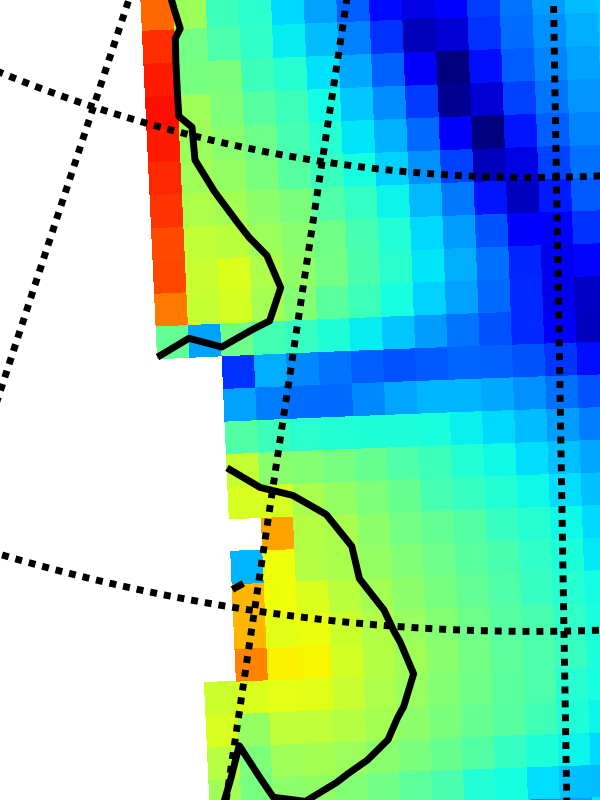
\includegraphics[width=1.65in,keepaspectratio=true]{g40km-detail} 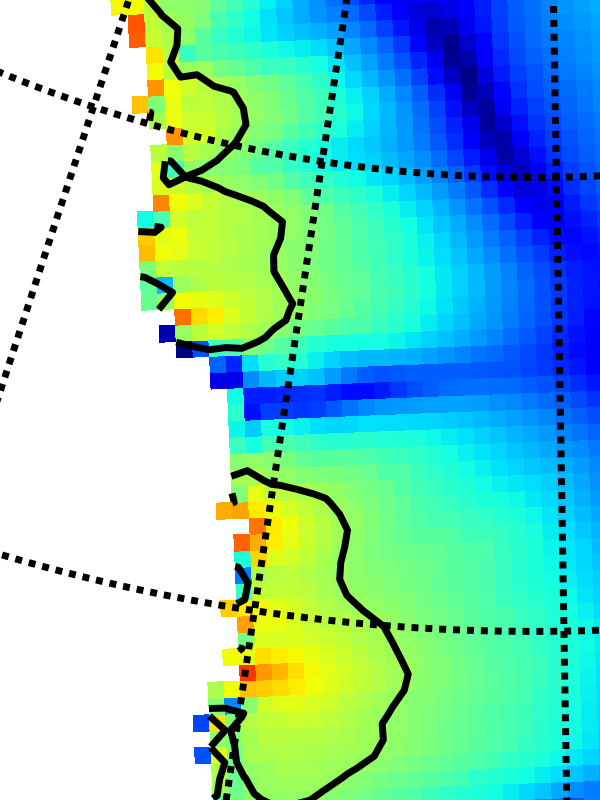
\includegraphics[width=1.65in,keepaspectratio=true]{g20km-detail} 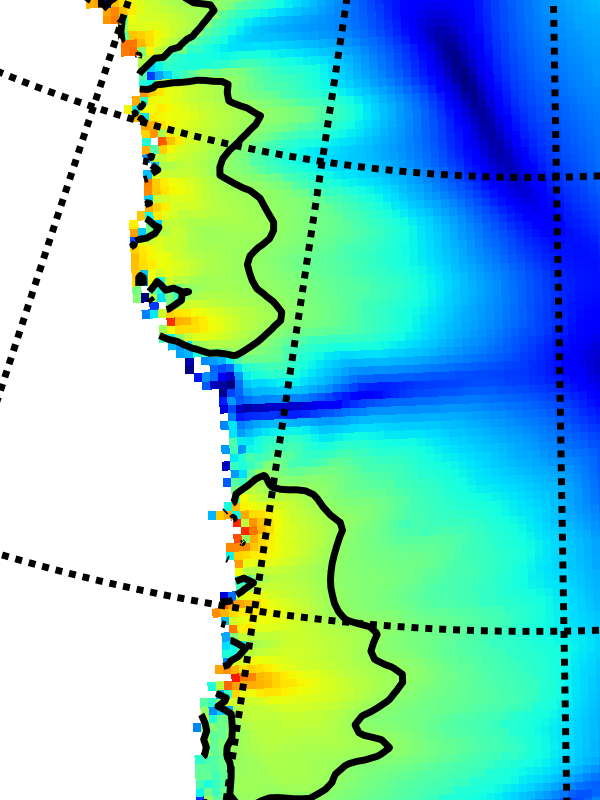
\includegraphics[width=1.65in,keepaspectratio=true]{g10km-detail} 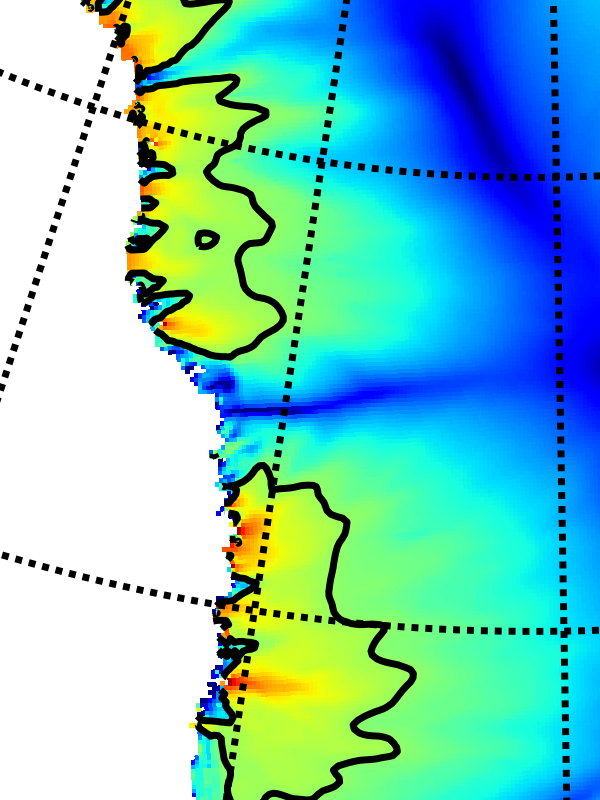
\includegraphics[width=1.65in,keepaspectratio=true]{g5km-detail} }
\caption{Detail of field \texttt{csurf} showing the central western coast of Greenland, including Jakobshavn Isbrae (lowest major flow), from runs of resolution 40, 20, 10, 5 km (left-to-right).  Color scheme and scale, including 100 m/a contour (solid black), are all identical to \texttt{csurf} Figures \ref{fig:secondoutputcoarse}, \ref{fig:csurfvsobserved}, and \ref{fig:secondoutputfiner}.}
\label{fig:gridseqdetail}
\end{figure}

Figure \ref{fig:gridseqdetail}, showing only a detail of the western coast of Greenland, with several outlet glaciers visible, suggests what is accomplished: the high resolution runs have separated outlet glacier flows, as they are in fact.  Note that all of these results were generated in a few wall clock hours on a laptop!  The surface speed \texttt{csurf} from files \texttt{g10km_gridseq.nc} and \texttt{g5km_gridseq.nc} is shown (two right-most subfigures).  In the two left-hand subfigures we show the same field from NetCDF files \texttt{g40km_10ka_hy.nc} and \texttt{g20km_10ka_hy.nc}; the former is an added 40 km result using an obvious modification of the run in section \ref{subsect:ssarun}.

\begin{figure}[ht]
\centering
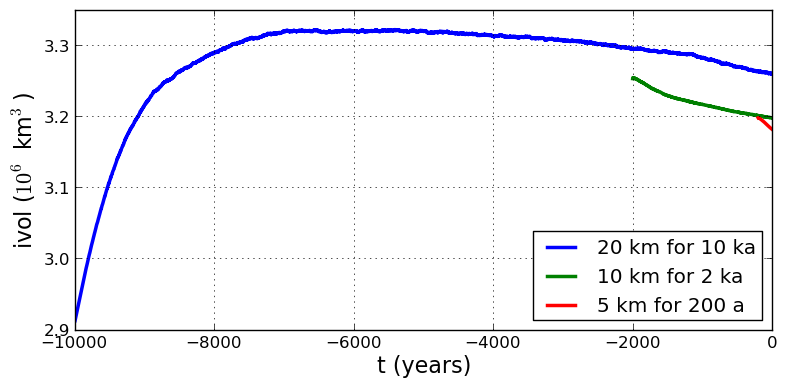
\includegraphics[width=4.5in,keepaspectratio=true]{ivol-gridseq}
\caption{Time series of ice volume \texttt{ivol} from the three runs in our grid sequencing example: 20 km for 10 ka = \texttt{ts_g20km_10ka_hy.nc}, 10 km for 2 ka = \texttt{ts_g10km_gridseq.nc}, and 5 km for 200 a = \texttt{ts_g20km_10ka_hy.nc}.}
\label{fig:ivolgridseq}
\end{figure}

Figure \ref{fig:ivolgridseq}, which shows time series of ice volume, also shows the cost of high resolution, however.  The short 200 a run on the 5 km grid took about 3 wall-clock hours compared to the 10 minutes taken by the 10 ka run on a 20 km grid.  The fact that the time series for ice volume on 10 km and 5 km grids are not very ``steady'' also suggests that these runs should actually be longer.

In this vein, if you have an available supercomputer then a good exercise is to extend our grid sequencing example to 3 km or 2 km resolutions \cite{AschwandenAdalgeirsdottirKhroulev}; these grids are already supported in the script \texttt{spinup.sh}.  Note that the vertical grid also generally gets refined as the horizontal grid is refined.

Going to a 1km grid is possible, but you will start to see the limitations of distributed file systems in writing the enormous NetCDF files in question \cite{DickensMorey2013}.  Notice that a factor-of-five refinement in all three dimensions, e.g.~from 5 km to 1 km in the horizontal, and from 20 m to 4 m in the vertical, generates an output NetCDF file which is 125 times larger.  Since the already-generated 5 km result \texttt{g5km_gridseq.nc} is over 0.5 Gb, the result is a very large file at 1 km.

On the other hand, on fine grids we observe that \emph{memory} parallelism, i.e.~spreading the stored model state over the separated memory of many nodes of supercomputers, is as important as the usual \emph{computation} (CPU) parallelism.

This subsection has emphasized the ``P'' in PISM, the nontrivial parallelism in which the solution of the conservation equations, especially the stress balance equations, is distributed across processors.  An easier and more common mode of parallelism is to distribute distinct model runs, each with different parameter values, among the processors.  For scientific purposes, such parameter studies, whether parallel or not, are at least as valuable as individual high-resolution runs.


\subsection{Getting serious II: an ice dynamics parameter study}  \label{subsect:paramstudy}

The readers of this manual should not assume the PISM authors know all the correct parameters for describing ice flow.  While PISM must have \emph{default} values of all parameters, to help users get started,\footnote{They are stored in human-readable form in the file \texttt{src/pism_config.cdl}.} it has more than two hundred user-configurable parameters.  The goal in this manual is to help the reader adjust them to their desired values.  While ``correct'' values may never be known, or may not exist, examining the behavior of the model as it depends on parameters is both a nontrivial and an essential task.

For some parameters used by PISM, changing their values within their ranges of experimental uncertainty is unlikely to affect model results in any important manner (e.g.~\texttt{sea_water_density}).  For others, however, for instance for the exponent in the basal sliding law, changing the value is highly-significant to model results, as we'll see in this subsection.  This is also a parameter which is very uncertain given current glaciological understanding \cite{CuffeyPaterson}.

To illustrate a parameter study in this Manual we restrict consideration to just two important parameters for ice dynamics,\begin{itemize}
\item $q=$ \texttt{pseudo_plastic_q}: exponent used in the sliding law which relates basal sliding velocity to basal shear stress in the SSA stress balance; see subsection \ref{subsect:basestrength} for more on this parameter, and
\item $e=$ \texttt{sia_enhancement_factor}: values larger than one give flow ``enhancement'' by making the ice deform more easily in shear than is determined by the standard flow law \cite{LliboutryDuval1985,PatersonBudd}; applied only in the SIA stress balance; see subsection \ref{sec:rheology} for more on this parameter.
\end{itemize}

By varying these parameters over full intervals of values, say $0.1\le q \le 1.0$ and $1 \le e \le 6$, we could explore a two-dimensional parameter space.  But of course each $(q,e)$ pair needs a full computation, so we can only sample this two-dimensional space.  Furthermore we must specify a concrete run for each parameter pair.  In this case we choose to run for 1000 model years, in every case initializing from the stored state \texttt{g10km_gridseq.nc} generated in the previous subsection \ref{subsect:gridseq}.

The next script, which is \texttt{param.sh} in \texttt{examples/std-greenland/}, gets values $q\in\{0.1,0.5,1.0\}$ and $e\in\{1,3,6\}$ in a double \texttt{for}-loop.  It generates a run-script for each $(q,e)$ pair.  For each parameter setting it calls \texttt{spinup.sh}, with the environment variable \texttt{PISM_DO=echo} so that \texttt{spinup.sh} simply outputs the run command.  This run command is then redirected into an appropriately-named \texttt{.sh} script file:
\begin{scriptvrb}
#!/bin/bash
NN=4
DUR=1000
START=g10km_gridseq.nc
for PPQ in 0.1 0.5 1.0 ; do
  for SIAE in 1 3 6 ; do
     PISM_DO=echo REGRIDFILE=$START PARAM_PPQ=$PPQ PARAM_SIAE=$SIAE \
       ./spinup.sh $NN const $DUR 10 hybrid p10km_${PPQ}_${SIAE}.nc \
       &> p10km_${PPQ}_${SIAE}.sh
  done
done
\end{scriptvrb}
%$
Notice that, because the stored state \texttt{g10km_gridseq.nc} used $q=0.5$ and $e=3$, one of these runs simply  continues with no change in the physics.

To set up and run the parameter study, without making a mess from all the generated files, do:
\small
\begin{verbatim}
$ cd examples/std-greenland/           # g10km_gridseq.nc should be in this directory
$ mkdir paramstudy
$ cd paramstudy
$ ln -s ../g10km_gridseq.nc            # these four lines make links to ...
$ ln -s ../pism_Greenland_5km_v1.1.nc  #
$ ln -s ../spinup.sh                   #
$ ln -s ../param.sh                    # ... existing files in examples/std-greenland/
$ ./param.sh
\end{verbatim}
\normalsize
The result of the last command is to generate nine run scripts,
\small
\begin{verbatim}
p10km_0.1_1.sh  p10km_0.1_3.sh  p10km_0.1_6.sh
p10km_0.5_1.sh  p10km_0.5_3.sh  p10km_0.5_6.sh
p10km_1.0_1.sh  p10km_1.0_3.sh  p10km_1.0_6.sh
\end{verbatim}
\normalsize
The reader should inspect a few of these scripts.  They are all very similar, of course, but, for instance, the \texttt{p10km_0.1_1.sh} script uses options \texttt{-pseudo_plastic_q 0.1} and \texttt{-sia_e 1}.

\begin{figure}[ht]
\centering
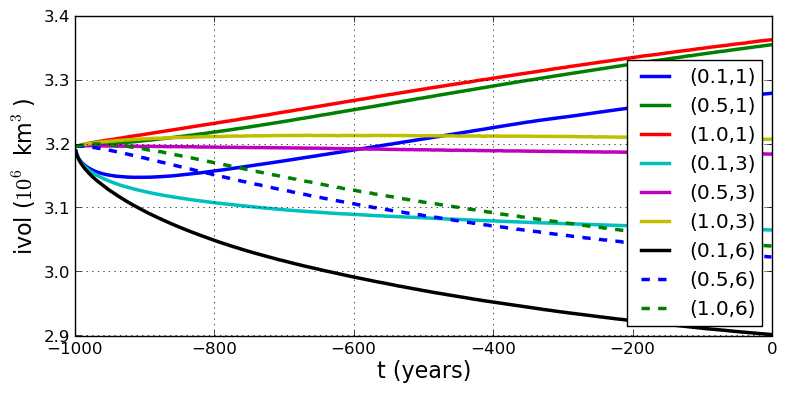
\includegraphics[width=4.5in,keepaspectratio=true]{ivol-param}

\caption{Time series of ice volume \texttt{ivol} from nine runs in our parameter study example, with parameter choices $(q,e)$ given.}
\label{fig:ivolparamstudy}
\end{figure}

We have not yet run PISM, but only asked one script to create nine others.  We now have the option of running them sequentially or in parallel.  Each script itself does a parallel run, over the \texttt{NN=4} processes specified by \texttt{param.sh} when generating the run scripts.  If you have $4 \times 9 = 36$ cores available then you can do the runs fully in parallel (this is \texttt{runparallel.sh} in \texttt{examples/std-greenland/}):
\begin{scriptvrb}
#!/bin/bash
for scriptname in $(ls p10km*sh) ; do
  echo ; echo "starting ${scriptname} ..."
  bash $scriptname &> out.$scriptname &  # start immediately in background
done
\end{scriptvrb}
%$
Otherwise you should do them in sequence (this is \texttt{runsequential.sh} in \texttt{examples/std-greenland/}):
\begin{scriptvrb}
#!/bin/bash
for scriptname in $(ls p10km*sh) ; do
  echo ; echo "starting ${scriptname} ..."
  bash $scriptname                       # will wait for completion
done
\end{scriptvrb}
%$
On the same old 2012-era 4 core laptop, \texttt{runsequential.sh} took a total of just under 7 hours to complete the whole parameter study.  The runs with $q=0.1$ (the more ``plastic'' end of the basal sliding spectrum) took up to four times longer than the $q=0.5$ and $q=1.0$ runs.  Roughly speaking, values of $q$ which are close to zero imply a subglacial till model with a true yield stres, and the result is that even small changes in overall ice sheet state (geometry, energy, \dots) will cause \emph{some} location to exceed its yield stress and suddenly change flow regime.  This will shorten the time steps.  By contrast, the $e$ value is much less significant in determining run times.

\begin{figure}[ht]
\centering
\mbox{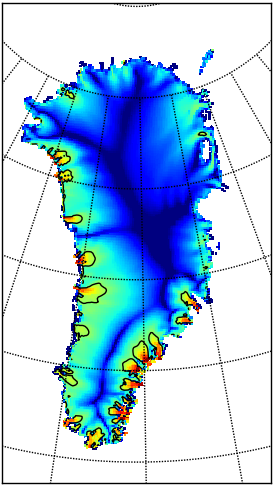
\includegraphics[height=2.6in,keepaspectratio=true]{p10km-01-1-csurf.png} 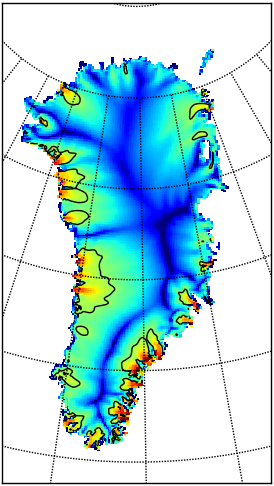
\includegraphics[height=2.6in,keepaspectratio=true]{p10km-01-3-csurf.png} 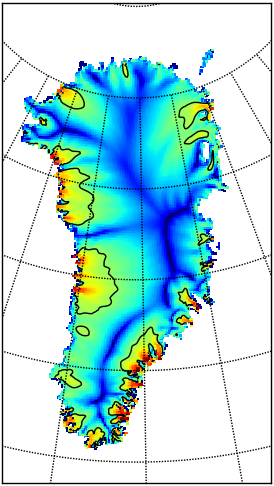
\includegraphics[height=2.6in,keepaspectratio=true]{p10km-01-6-csurf.png} \qquad \hspace{1.87in}}

\mbox{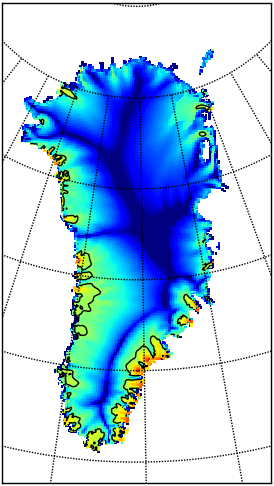
\includegraphics[height=2.6in,keepaspectratio=true]{p10km-05-1-csurf.png} 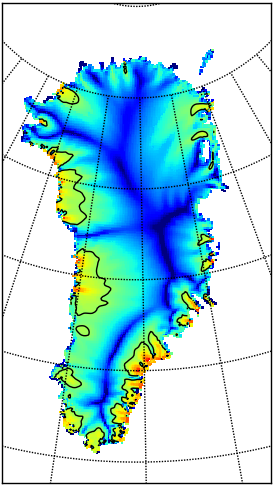
\includegraphics[height=2.6in,keepaspectratio=true]{p10km-05-3-csurf.png} 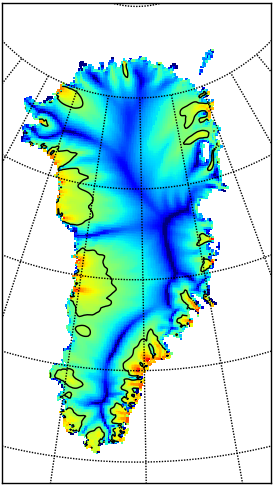
\includegraphics[height=2.6in,keepaspectratio=true]{p10km-05-6-csurf.png} 
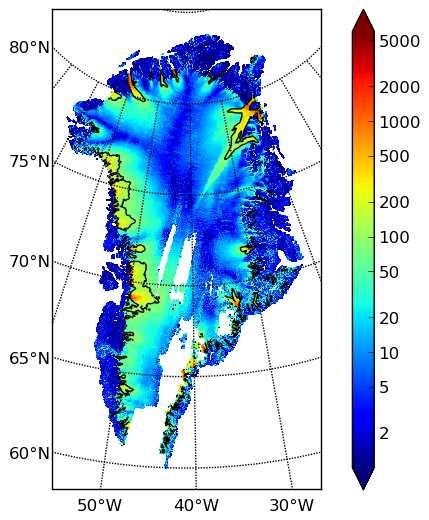
\includegraphics[height=2.7in,keepaspectratio=true]{Greenland-5km-v1p1-surfvelmag}}
\smallskip

\mbox{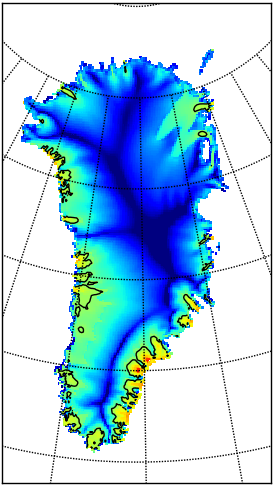
\includegraphics[height=2.6in,keepaspectratio=true]{p10km-1-1-csurf.png} 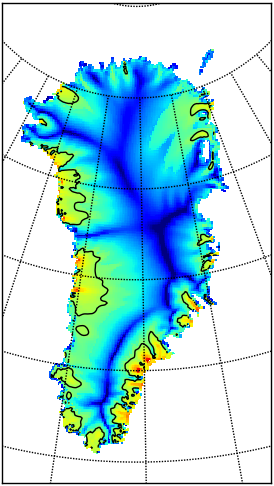
\includegraphics[height=2.6in,keepaspectratio=true]{p10km-1-3-csurf.png} 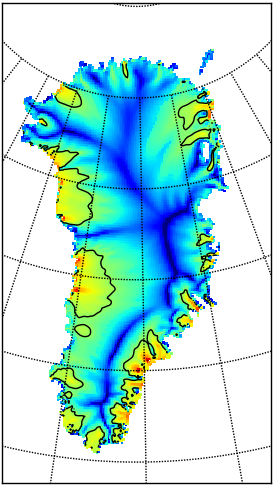
\includegraphics[height=2.6in,keepaspectratio=true]{p10km-1-6-csurf.png} \qquad \hspace{1.87in}}

\caption{Surface speed \texttt{csurf} from a 10 km grid parameter study.  Right-most subfigure is observed data from \texttt{Greenland_5km_v1.1.nc}.  Top row: $q=0.1$ and $e=1,3,6$ (left-to-right).  Middle row: $q=0.5$.  Bottom row: $q=1.0$.  All subfigures have common color scale (velocity m/a), as shown in the right-most figure, with 100 m/a contour shown in all cases (solid black).}
\label{fig:paramstudy}
\end{figure}

On a supercomputer, the \texttt{runparallel.sh} script generally should be modified to submit jobs to the scheduler.  See example scripts \texttt{advanced/paramspawn.sh} and \texttt{advanced/paramsubmit.sh} for a parameter study that does this.  (But see your system administrator if you don't know what a ``job scheduler'' is!)  Of course, if you have a supercomputer then you can redo this parameter study on a 5 km grid.

Results from these runs are seen in Figures \ref{fig:ivolparamstudy} and \ref{fig:paramstudy}.  In the former we see that the $(0.5,3)$ run simply continues the previous initialization run.  In some other graphs we see abrupt initial changes, caused by abrupt parameter change, e.g.~when the basal sliding becomes much more plastic ($q=0.1$).  In all cases with $e=1$ the flow slows and the sheet grows in volume as discharge decreases, while in all cases with $e=6$ the flow accelerates and the sheet shrinks in volume as discharge increases.

In Figure \ref{fig:paramstudy} we can compare the surface speed model results to observations.  Roughly speaking, the ice softness parameter $e$ has effects seen most-clearly by comparing the interior of the ice sheet; scan left-to-right for the $e=1,3,6$ subfigures.  The basal sliding exponent $q$ has effects seen most-clearly by comparing flow along the very steep margin, especially in the southern half of the ice sheet; scan top-to-bottom for $q=0.1,0.5,1.0$, going from nearly-plastic at top to linear at bottom.

From such figures we can make an informal assessment and comparison of the results, but objective assessment is important.  Example objective functionals include: \emph{(i)} compute the integral of the square (or other power) of the difference between the model and observed surface velocity \cite{AschwandenAdalgeirsdottirKhroulev}, or \emph{(ii)} compute the model-observed differences between the histogram of the number of cells with a given surface speed \cite{BKAJS}.  Note that these functionals are measuring the effects of changing a small number of parameters, namely two parameters in the current study.  So-called ``inversion'' might use the same objective functionals but with a much larger parameter space.  Inversion is therefore capable of achieving much smaller objective measures \cite{Habermannetal2013,Larouretal2012,Priceetal2011}, though at the cost of less understanding, perhaps, of the meaning of the optimal parameter values.

\clearpage  % does not lengthen pages, and puts Figure \ref{fig:paramstudy} before Table \ref{tab:NetCDFview}

\subsection{Handling NetCDF files}\label{subsect:nctoolsintro}  PISM takes one or more NetCDF files as input, then it does some computation, and then it produces one or more NetCDF files as output.  Usually, other tools help to extract meaning from these NetCDF files, and yet more tools help with creating PISM input files or post-processing PISM output files.  Thus we conclude this Getting Started section with a list of some NetCDF tools in Table \ref{tab:NetCDFview}.

We frequently use \texttt{ncview} and ``\texttt{ncdump -h}'' for quick visualization and metadata examination.  NCO has powerful command-line manipulation of NetCDF files, but requires some learning.  Often python scripts (using the \texttt{netcdf4-python} package; see the PISM Installation Manual), or Matlab or other languages, are the fastest way to fix up a NetCDF file or extract fields from it.  To use CDO on PISM files, first run the script \texttt{nc2cdo.py}, from the \texttt{util/} PISM directory, on the file.  This fixes the metadata so that CDO will understand the mapping.

See Table \ref{tab:modelhierarchy} in subsection \ref{sec:model-hierarchy} for an overview on the data necessary for modeling.  For more information on the format of input files for PISM, see section \ref{sec:initboot}.

\newcommand{\netcdftool}[1]{#1\index{NetCDF!tools!#1}}
\begin{table}[ht]
\centering
\small
\begin{tabular}{llp{0.45\linewidth}}
  \toprule
  \textbf{Tool} & \textbf{Site} & \textbf{Function} \\
  \midrule
  & \url{www.unidata.ucar.edu/software/netcdf/} & root for NetCDF information \\
  \midrule
  \netcdftool{\texttt{ncdump}} & \emph{included with any NetCDF distribution} & dump binary NetCDF as \texttt{.cdl} (text) file \\
  \netcdftool{\texttt{ncgen}} & \emph{included with any NetCDF distribution} & convert \texttt{.cdl} file to binary NetCDF \\
  \midrule
  \netcdftool{CDO} & \url{http://code.zmaw.de/projects/cdo} & = Climate Data Operators; command-line tools, including conservative re-mapping \\
  \netcdftool{IDV} & \url{http://www.unidata.ucar.edu/software/idv/} & more complete visualization \\
  \netcdftool{NCO}\index{NCO (NetCDF Operators)} & \url{http://nco.sourceforge.net/} & = NetCDF Operators; command-line tools\\
  \netcdftool{NCL} &  \url{http://www.ncl.ucar.edu} & = NCAR Command Language\\
  \netcdftool{\texttt{ncview}} & \href{http://meteora.ucsd.edu/~pierce/ncview_home_page.html}{\texttt{meteora.ucsd.edu/$\sim$pierce}} & quick graphical view \\
  \netcdftool{PyNGL} &  \url{http://www.pyngl.ucar.edu} & Python version of NCL\\
  \bottomrule
\end{tabular}
\normalsize
\caption{A selection of tools for viewing and modifying NetCDF files.}
\label{tab:NetCDFview}
\end{table}


%%% Local Variables: 
%%% mode: latex
%%% TeX-master: "manual"
%%% End: 


% LocalWords:  metadata SPECMAP paleo html IDV



\clearpage
\newpage
\section{Ice dynamics, the PISM view}\label{sect:dynamics}

\subsection{PISM design principles}\index{PISM!principles}  This section gives an overview of ice dynamics models in PISM.  First, some organizing principles:
\begin{enumerate}
\item source code should be open, free, and work well with other free software tools,
\item science is better if done with publicly-available data,
\item numerical methods should be verifiable (i.e.~compare to exact solutions of the modeled equations),
\item shallow models are (currently) the most effective at whole ice sheet scale,
\item comparing results from a hierarchy of ice dynamics simplifications is more valuable than getting them from any particular model equations,
\item everything computed diagnostically (instantaneously) should be available prognostically (i.e.~it can evolve in time), and
\item climate inputs should affect ice dynamics by a well-defined interface.
\end{enumerate}

\noindent We do not claim to follow these principles perfectly, but principle 1 is illustrated by our existence and principle 2 by examples in sections \ref{sect:start}, \ref{sec:eismint-greenland}, and \ref{sect:ross}.  Principle 3 is addressed in section \ref{sect:verif}.  Principles 4, 5, 6, and 7 are addressed next.


\subsection{Two main shallow models, SIA and SSA}\index{PISM!SIA}\index{PISM!SSA}  At each time-step of a typical PISM run, the geometry, temperature, and basal strength of the ice sheet are included into stress (momentum) balance equations to determine the velocity of the flowing ice.   The ``full'' stress balance equations, namely the (non-Newtonian) Stokes model for slowly-flowing fluids \cite{Fowler}, are themselves an inertia-free approximation of the conservation of momentum equations.  Even though PISM does not solve this ``full'' model, it can numerically solve two different shallow approximations which are suited to the situations in large ice sheet and ice shelf systems:
\begin{itemize}
\item the non-sliding shallow ice approximation (SIA)\index{SIA (shallow ice approximation)} \cite{Hutter}, also called the ``lubrication approximation'' \cite{Fowler}, which describes ice as flowing by shear in planes parallel to the geoid, with a strong contact of ice base to bedrock, and
\item the shallow shelf approximation (SSA)\index{SSA (shallow shelf approximation)} \cite{WeisGreveHutter}, which describes a membrane-type flow of floating ice \cite{Morland}, or grounded ice which is sliding over a weak base \cite{MacAyeal,SchoofStream}.
\end{itemize}
PISM solves both the SIA and SSA equations in parallel.  Time-stepping solutions of the mass continuity and energy conservation equations are possible when using each model.

The SIA\index{SIA (shallow ice approximation)!applicability} equations are, as a rule, easier and quicker to numerically solve than the SSA, and they are also easier to parallelize.\index{parallelization!relative ease of, between SIA and SSA}  They describe the shear as a local function of the driving stress of classical glaciology \cite{Paterson}.  They can confidently be applied to those grounded parts of ice sheets for which the basal ice is frozen to the bedrock, or minimally sliding, and for which the bed topography is relatively slowly-varying in the map-plane \cite{Fowler}.  These characteristics apply to the majority \emph{by area} of the Greenland and Antarctic ice sheets.  We recommend solving the SIA with a completely \emph{non-sliding} base because the ad~hoc addition of ``sliding laws''\index{SIA (shallow ice approximation)!sliding laws} into the SIA stress balance, and especially schemes which ``switch on'' at the pressure-melting temperature \cite{EISMINT00}, have bad continuum and numerical modeling consequences \cite[appendix B]{BBssasliding}.

The SSA\index{SSA (shallow shelf approximation)!applicability} equations, by contrast, can confidently be applied to large floating ice shelves, which have small depth-to-width ratio and negligible basal resistance \cite{Morland,MorlandZainuddin}.  The flow speeds in ice shelves are frequently an order-of-magnitude higher than in the non-sliding, grounded parts of ice sheets, and this speed contrast is easily seen in comparing the solutions of SIA and SSA models.

Terrestrial ice sheets also have fast-flowing grounded parts, however, called ``ice streams'' or ``outlet glaciers'' \cite{TrufferEchelmeyer}.  Such features appear at the margin of, and sometimes well into the interior of, the Greenland \cite{Joughinetal2001}\index{Ice Sheets!Greenland ice sheet} and Antarctic \cite{BamberVaughanJoughin}\index{Ice Sheets!Antarctic ice sheet} ice sheets.  Describing these faster-flowing grounded parts of ice sheets requires, at least, something more than the non-sliding SIA because adjacent columns of ice which have different amounts of basal resistance exert strong ``longitudinal'' or ``membrane'' stresses \cite{SchoofStream} on each other.  One might use the full Stokes equations, or a ``higher-order'' model (which still uses some shallow approximations \cite{Blatter,Pattyn03}), but this immediately leads to a resolution-versus-stress-inclusion tradeoff because the amount of computation per map-plane grid location is so much higher in these models.  Also, with any stress balance model one must still specify an appropriate sliding boundary condition, and uncertainty in this boundary condition may (and usually does) dominate the modeling error made by not including higher-order stresses in the balance.

If the fast-flowing grounded ice is sufficiently shallow, in the usual aspect-ratio sense, then the SSA model can be applied.  The best-known combination of the SSA model with a choice of basal resistance model is the Siple Coast (Antarctica) ice stream model by MacAyeal\index{People!MacAyeal, Doug} \cite{MacAyeal}, who used a linearly-viscous model for the underlying till.  A free boundary problem with the same (SSA) balance equations is the Schoof\index{People!Schoof, Christian} \cite{SchoofStream} model of ice streams, using a plastic (Coulomb) sliding relation.  In this model ice streams appear where there is ``till failure'' \cite{Paterson}---the basal shear stress exceeds the yield stress imposed as a boundary condition---and the location of ice streams is not imposed in advance.

As noted, both the SIA and SSA models are \emph{shallow} approximations.  More precisely, these model equations are derived from the Stokes equations by different small-parameter arguments, both based on a small depth-to-width ratio for the ice sheet.  Both models, and ``higher order'' models as well, approximate the pressure as hydrostatic.  For the small-parameter argument in the SIA case see \cite{Fowler}.  For the corresponding SSA argument, see \cite{WeisGreveHutter} or the appendices of \cite{SchoofStream}.  Schoof and Hindmarsh \cite{SchoofHindmarsh} have analyzed the connections between these shallowest models and ``higher order'' models, while \cite{GreveBlatter2009} discusses ice dynamics and stress balances comprehensively.

In PISM the SSA may be used as a ``sliding law'' for grounded ice which is already modeled everywhere by the non-sliding SIA \cite{BBssasliding}.  In brief, our concept for grounded ice is that, in addition to including shear in planes parallel to the geiod, we must balance the membrane stresses which become important anywhere there is significant sliding, and this inclusion is especially important when there are changes in basal strength, both spatial and temporal.  The more traditional use of ``sliding laws'' in pure-SIA models does not incorporate this basic physical truth \cite{Fowler01}.

The resulting ``SIA+SSA hybrid'' model is recommended by the PISM developers for most whole ice sheet modeling purposes because it seems to be a good compromise given currently available data and computational power (see \cite{BKAJS,Martinetal2010TCD,Winkelmannetal2010TCD}, for example).  This ``sliding law'' role for the SSA is in addition to its more obvious role in ice \emph{shelf} modeling, and so the SSA plays both roles in a PISM whole ice sheet model if there are large floating ice shelves--- as in Antarctica \cite{Martinetal2010TCD,Winkelmannetal2010TCD}.

By default, PISM does not numerically solve the SSA because any such solution must go with a conscious user choice about basal strength.  The user must both use a command-line option to turn on the SSA (section \ref{subsect:ssacontrol}) and also make choices in input files and runtime options about basal strength (section \ref{subsect:basestrength}).


\subsection{A hierarchy of simplifying assumptions for grounded ice flow}
\label{sec:model-hierarchy}\index{PISM!hierarchy of simplifying assumptions}

Table \ref{tab:modelhierarchy} describes a hierarchy of models, listed in order of increasing effectiveness in modeling grounded ice sheets with fast flow features.  This is also the order of increasing need for data to serve as boundary and initial conditions, an important consideration for the scientific user.

As an additional row for such a table, one might list ``full Stokes''.  That stress balance is \emph{not} planned for PISM at any time, however, as its numerical solution requires a fundamentally different computational architecture.

It makes sense to also talk about an \emph{ice shelf} model hierarchy, and even about a special hierarchy of models for the transition from grounded to floating ice \cite{SchoofMarine1}, but this would take us too far afield.  Currently, ice shelves should always be modeled by the SSA equations in PISM.  See section \ref{sect:ross}.

Although it begins to expose the internals of PISM, we think it is also helpful to see the implemented stress balances as PISM software components (C++ classes).  Figure \ref{fig:stressbalance} shows that the sequence of actions taken by SIA-only, SSA-only, and SIA+SSA hybrid models is, in some sense, the same: a membrane stress solution first, a distribution of vertical shear in the column of ice second, and a use of incompressibility to compute the vertical component of the velocity third.  The nonsliding SIA-only model has a degenerate first step and the SSA-only model has a degenerate second step.  The hybrid model described by Pollard and deConto \cite{PollardDeConto}, for another example, would add the shear in the column in a different manner (than in the current implementation, following \cite{BBssasliding,Winkelmannetal2010TCD}).

\newenvironment{tightlist}{\begin{itemize}  \vspace{-0.15in}\addtolength{\itemsep}{-0.5\baselineskip} } {\vspace{-0.1in} \end{itemize}}

%\newcommand{\nolist}[1]{\begin{tightlist} \item[] [\emph{#1}] \end{tightlist}}
\newcommand{\nolist}[1]{[\emph{#1}] \vspace{0.1in}}

\begin{table}[ht]
\caption{Hierarchy of current and planned flow models in PISM, for the grounded
  parts of ice sheets, from most to fewest simplifying assumptions \emph{and}
  from least to greatest need for boundary data.  The \emph{italicized} models
  are planned for future versions of PISM but are not implemented so far..}\label{tab:modelhierarchy} 
\small\medskip
\begin{tabular}{p{0.22\linewidth}p{0.40\linewidth}p{0.32\linewidth}}\hline
\textbf{Model} & \textbf{Assumptions} & \textbf{Required data} \\ \hline
\vspace{2mm}  \emph{perfectly-plastic ice} \small & \vspace{2mm}\emph{steady state}; ice has shear stresses at or below a pre-determined ``yield stress''; requires location of ice sheet margin  \vspace{2mm} & \vspace{2mm} \begin{tightlist} \item bed elevation\end{tightlist} \\
\emph{balance velocities} \small & \emph{steady state}; ice flows down surface gradient \cite{JoughinetalGrBal97} & \nolist{same as above, plus:}  \begin{tightlist} \item surface mass balance \item initial ice thickness \end{tightlist} \\
\textsc{isothermal SIA} & non-sliding lubrication flow, fixed softness \cite{BLKCB,EISMINT96} & \nolist{same as above, but time-dependence is allowed} \\
\textsc{thermo-coupled SIA} & non-sliding lubrication flow, temperature-dependent softness \cite{BBL,EISMINT00} & \nolist{same as above, plus:} \begin{tightlist} \item surface temperature \item geothermal flux \end{tightlist} \\
\textsc{polythermal SIA} & same, but allowing $>0$ liquid water in temperate ice; conserves energy better \cite{AschwandenBuelerKhroulevBlatter,Greve} \vspace{2mm} & \nolist{same as above} \\
\textsc{SIA + SSA hybrid} & SSA as a sliding law for thermo-coupled SIA \cite{BBssasliding}; polythermal is the default & \nolist{same as above, plus:} \begin{tightlist} \item basal layer (``till'') strength \end{tightlist} \\
\emph{Blatter-Pattyn} \small & ``higher-order'', bridging stresses \cite{Blatter,Pattyn03,SchoofCoulombBlatter} & \nolist{same as above} \\ \hline
\end{tabular}
\normalsize
\end{table}


\subsection{Evolutionary and diagnostic modeling} \label{subsect:basicmodes}\index{PISM!evolution run}\index{PISM!diagnostic run}    The main goal of a numerical ice sheet model like PISM is to be a dynamical system which evolves over time as similarly as possible to the modeled ice sheet.  Such a goal assumes one has the right climate inputs and parameter choices at each time step.  For predictive purposes, it also assumes one has the right initial conditions, adequately describing the present state of the ice sheet.  This last assumption is rarely satisfied.  Instead, heuristics must be used to minimally-initialize an ice sheet model, before a possible stage of paleo-climate driven spin-up; see section \ref{sect:boot}.

Underlying an ice sheet model like PISM are evolution-in-time partial differential equations.  PISM solves these by taking small time steps.  ``Small'' time steps vary from hundredths to many model years, depending primarily on grid resolution and modeled ice flow speed.  Time steps are chosen adaptively in PISM, according to the stability criteria of the several numerical methods.

However, much ice flow modeling, especially of streams and shelves, uses only instantaneous ``diagnostic'' solution of the partial differential equations which determine the velocity field.  The models in PISM can produce such ``instantaneous'' velocity fields because of the slowness of the ice, in the sense that inertia can be neglected in the stress balance \cite{Fowler}.  The goal of a ``diagnostic run'' is usually to compute this velocity field, especially its observable surface values.  For example, a diagnostic run might be the ``forward model'' step in inverting surface velocities for basal strength\dots but that is beyond the scope of this \emph{Manual}.

Sections \ref{sec:eismint-greenland} and \ref{sect:ross} are examples illustrating evolutionary and diagnostic modeling modes of PISM.  The first of these describes time-stepping evolution models for the Greenland ice sheet, while the second describes a diagnostic SSA model for the Ross ice shelf.


\begin{figure}
  \centering
  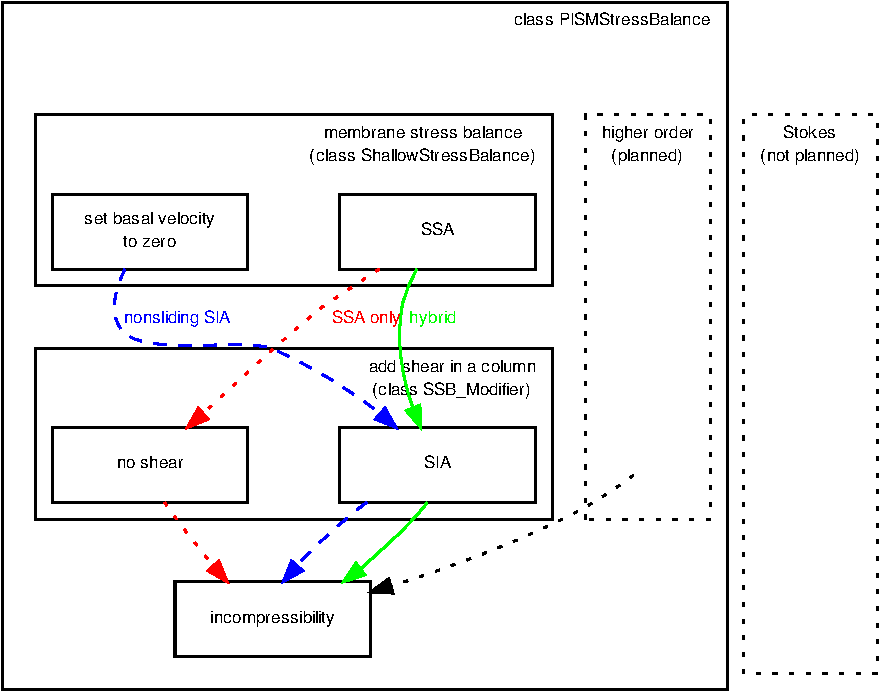
\includegraphics[width=6in]{stressbalance}
  \caption{The SIA-only, SSA-only, and SIA+SSA hybrid models represent different ``routes'' through stress balance PISM components.  In each case the inputs are ice geometry and boundary stresses, and the final output is a three-dimensional velocity field within the ice.}
  \label{fig:stressbalance}
\end{figure}


\subsection{Climate inputs, and their interface with ice dynamics}
\label{sec:climate-inputs}  

Because PISM's job is to approximate ice flow, its ``world view'' is centered around ice dynamics.  The discussion of boundary conditions, in this \emph{Manual} is necessarily ``ice-centric'' in our description here, but there is no constraint on the nature of, or completeness of, climate models which could be coupled to PISM.  This section applies the PISM organizing principle above (section \ref{sect:dynamics}): \emph{climate inputs affect ice dynamics by a well-defined interface}.

Figure~\ref{fig:climate-inputs} illustrates that any PISM ice sheet model has an interface (green) to a surface processes layer containing snow, firn, and liquid (or refrozen) runoff, and to the ocean (blue) if there is floating ice.  The surface processes layer might be very simple.  If it is ``owned'' by the PISM model then there is an additional interface (red) to the atmosphere above.  The interface to the surface layer is assumed in PISM to cover the whole surface of the ice, including ablation areas and even ice-free land.  Table \ref{tab:ice-dynamics-bc} lists fields which are needed as boundary conditions at the interfaces.

\begin{figure}
  \centering
  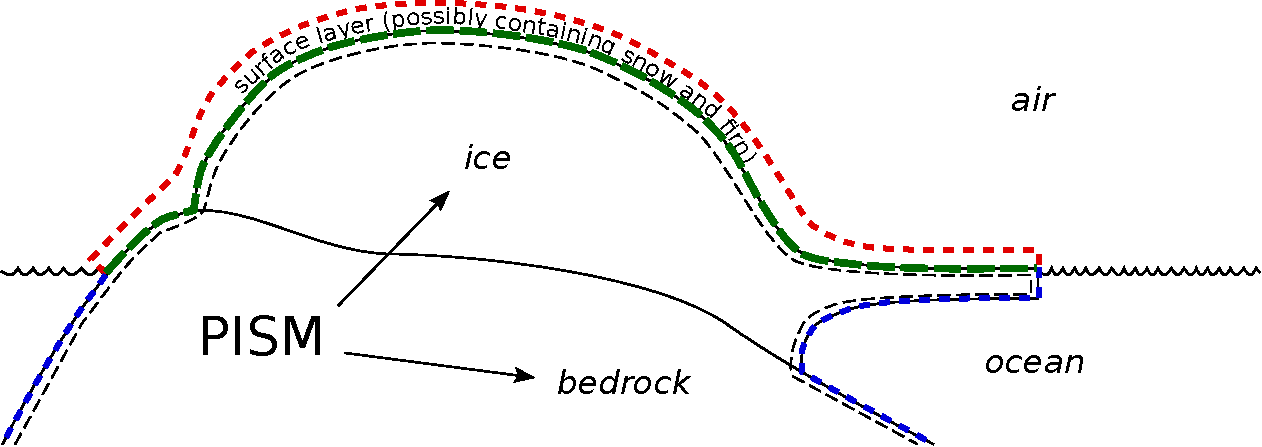
\includegraphics[width=6in]{figs/climate-cartoon.pdf}
  \caption{PISM's view of interfaces between an ice sheet and the outside world}
  \label{fig:climate-inputs}
\end{figure}

\begin{table}[h]
  \centering
  \begin{tabular}{p{0.35\linewidth}p{0.55\linewidth}}\\
    \hline
    \textbf{Boundary} & \textbf{Necessary conditions}\\
    \hline
    Top ice surface (below firn) (\textcolor{green}{green})& Ice temperature (or enthalpy) and mass flux into the ice\\
    Bottom surface of the thermal bed layer (not shown) & Geothermal flux\\
    Ice shelf basal surface (\textcolor{blue}{blue})& Mass flux into the ocean and ice boundary temperature\\
   \hline
  \end{tabular}
  \caption{Boundary conditions required by PISM's ice dynamics core; see figure
  \ref{fig:climate-inputs}}
  \label{tab:ice-dynamics-bc}
\end{table}

Regarding the base of the ice, as described in section \ref{subsect:beddef} PISM also includes an optional bed deformation component approximating the movement of the Earth's crust and upper mantle in response to changing ice load.   Furthermore the temperature of the layer of bedrock in contact with grounded ice is included in the conservation of energy model.  In this sense everything below the black dashed line (i.e.~ice and bedrock) is ``owned'' by PISM.  This fact adds two more boundary interfaces for the ice dynamics core: sub-ice-shelf/ocean (shown in blue) and the bottom of the bedrock thermal layer (not shown).

The PISM ice dynamics core would like to be able to get fields listed in Table
\ref{tab:ice-dynamics-bc} directly from observations or measurements, or directly from a GCM.  In many realistic modeling situations, however, PISM code must be used for all or part of the surface processes modeling necessary to provide the ice-dynamics core with the ``right'' fields.  Due to differences in model resolutions and required down-scaling, this need for some PISM-based boundary-processes modeling includes cases where PISM is coupled to a GCM.  In the kind of ``offline'' runs described in this \emph{Manual}, boundary processes are modeled, even if trivially.

Thus, to be able to use the data that \emph{is} available, an ice-sheet model has to
have additional components that are responsible for modeling surface (snow)
processes or sub-shelf/ocean interaction.  These components might be very minimal, merely turning data that we already have into data in the right units and with the right metadata, so that PISM knows what to do with it, for example.

Thus we have PISM's design: the ice-dynamics-and-earth-deformation PISM
core does not contain any parameterization or other model for boundary mass or
energy balance.  These boundary parameterizations and models are present in the PISM source code, however, as instances of \emph{PISMComponent} classes.  This simplifies customizing and debugging PISM's climate
inputs, promotes code reuse.  Moreover, it isolates the code that needs to be changed to
couple PISM to a climate model.

Users wishing to customize PISM's climate inputs should see the \emph{PISM
  Source Browser}, e.g.~at
\url{\PISMBROWSERURL} and the documentation
of \emph{PISMSurfaceModel}, \emph{PISMAtmosphereModel} and
\emph{PISMOceanModel} therein.  Also, section \ref{sec:eismint-greenland} describes a
modeling example using a non-standard air temperature parameterization. Looking
at source files \texttt{pgrn.cc} and \texttt{pgrn_atmosphere.cc} may be a reasonable
start.

Note that figure~\ref{fig:climate-inputs} includes an interface between the surface layer and the air (red dashed line).
Unlike the ones listed in table~\ref{tab:ice-dynamics-bc}, this interface
\emph{may not even be present in some PISM configurations:} the ice dynamics
core of PISM only ``knows'' about mediums bordering ice and bedrock. A pair
consisting of a \emph{PISMSurfaceModel} and a \emph{PISMOceanModel} may be
hiding anything from a nearly trivial parameterization of ice surface
temperature plus surface and sub-shelf mass fluxes to a GCM of great
complexity.

Figure~\ref{fig:climate-input-data-flow} illustrates the corresponding data
flow \emph{into} the PISM core; the data flow in the other direction depends on
particular modeling choices.

This figure requires an explanation: a ``modifier'' in this context is an
adjustment of climate inputs that can be used with different climate
choices.  Using ice-core-derived air temperature offsets to model the space-time distribution of paleo surface temperature is an example.  Note that PISM has a generic ``forcing'' mechanism that can be paired with another model. Please see section \ref{sec:boundary-models} for
a list of climate components included in PISM source code and other details.

\begin{figure}
  \centering
  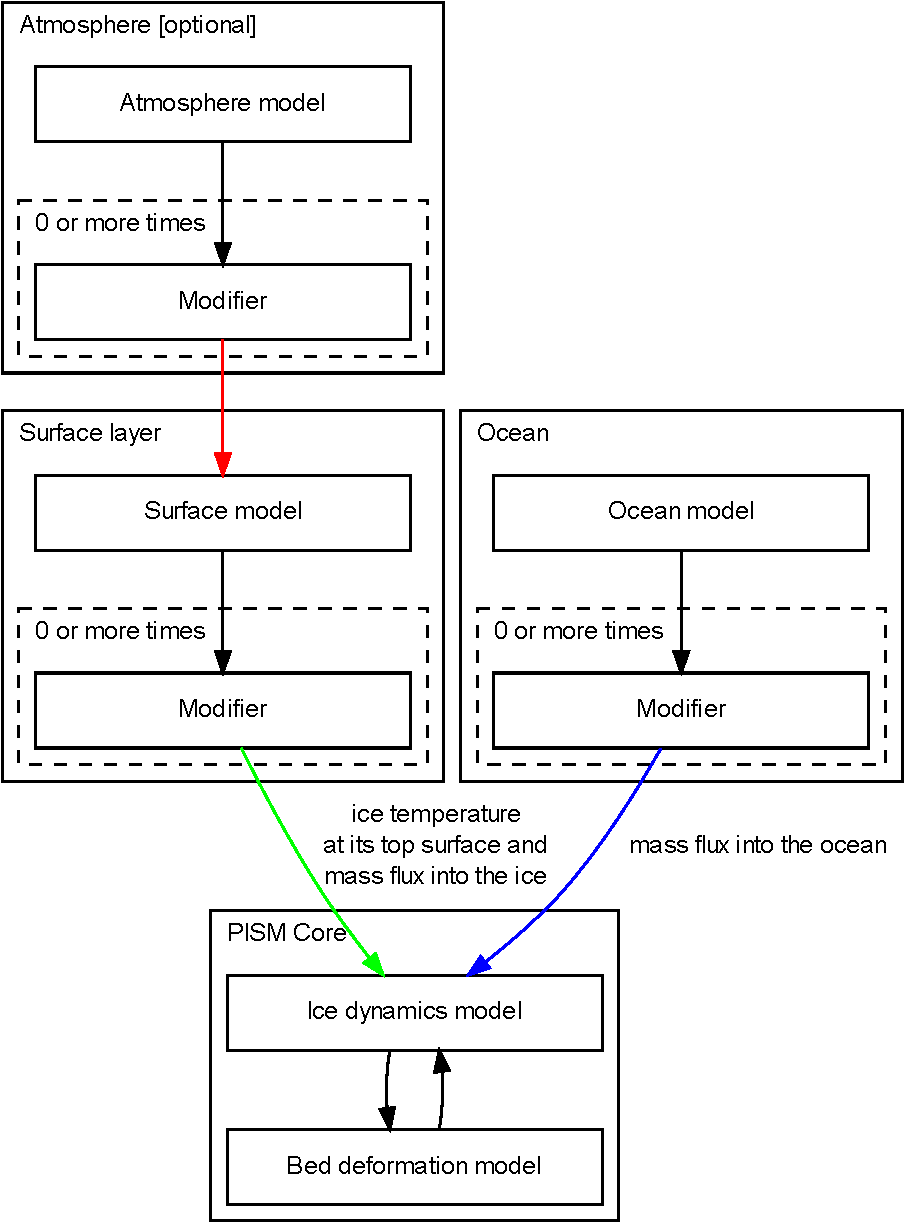
\includegraphics[width=5in]{figs/data-flow.pdf}
  \caption{PISM climate input data flow. Colored arrows correspond to interfaces in
    figure \ref{fig:climate-inputs}.}
  \label{fig:climate-input-data-flow}
\end{figure}

Why describe this structure here? On the one hand, some users may be interested
in coupling PISM to other models. On the other hand, the PISM authors do not
claim expertise in modeling atmosphere, ocean, or even snow processes.   So the
separation has a code-reliability purpose. Indeed PISM users need to know that
they are ultimately responsible for providing the climate inputs they intend.
The auxiliary tool \texttt{pclimate}, described in subsection
\ref{subsect:pclimate}, is intended to help users observe the climate inputs
they have chosen, without involving ice dynamics at all.

\clearpage
\newpage
\section{Initialization and bootstrapping}
\label{sect:boot}  


There are three ways to start PISM,\begin{itemize}
\item the executables \texttt{pisms} and \texttt{pismv} initialize simplified-geometry experiments and verification tests, respectively, from formulas in the source code,
\item \texttt{-i} reads a previously-saved PISM model state, a NetCDF file, and
\item \texttt{-boot_file} reads an ``incomplete'' NetCDF file and uses heuristics to fill in needed fields.
\end{itemize}
Realistic modeling usually starts with the \texttt{-boot_file} option because real ice sheet observations are never complete initial conditions for ice sheet models.

\subsection{Initialization from a saved model state}  ``Initialization''\index{initialization!from saved model state} has a specific, simple meaning in PISM.  If a previous PISM run has saved a NetCDF file using ``\texttt{-o}'' then that file will contain complete initial conditions for continuing the run.  The output file from the last run can be loaded with ``\texttt{-i}'': \index{executables!\texttt{pisms}}

\begin{verbatim}
$ pisms -eisII A -y 100 -o foo.nc
$ pisms -eisII A -i foo.nc -y 100 -o bar.nc
\end{verbatim}
\smallskip

Note that simplified-geometry experiments (section \ref{sect:simp}) and verification tests (section \ref{sect:verif}) do not need input files at all because they initialize from formulas in the source code.  They can be continued from saved model states using \texttt{-i}.  As in the above example, however, specifying the simplified geometry experiment or verification test \emph{is} necessary, so that the run can continue with the climate inputs for that experiment or test.  For example, based on the above \texttt{pisms} runs, it is valid to do ``\texttt{\$ pismr -i foo.nc -y 100 -o bar.nc ...}'' but the climate and other parameters us PISM default values, and thus are not (necessarily) the values specified in EISMINT II.

As a technical but important note about saved states, a PISM run with \texttt{-ssa_floating_only} or \texttt{-ssa_sliding}
also saves the last SSA velocities to the output file, in variables 
\texttt{ubar_ssa} and \texttt{vbar_ssa}. The presence
of these velocities adds efficiency in restarting.  If you want a PISM restart to
ignore these velocities use \texttt{-dontreadSSAvels}.

\subsubsection*{\texttt{-i} file format}
PISM produces\footnote{Or, more accurately, attempts to produce; please let us know about violations you come across.} CF-1.4 compliant NetCDF\index{PISM!NetCDF file format}\index{NetCDF} files.  The easiest way to learn the output format \emph{and} the \texttt{-i} format is to do a simple run and then look at the metadata in the resulting file, like this:
\begin{verbatim}
$ pisms -eisII A -y 10 -o foo.nc
$ ncdump -h foo.nc | less
\end{verbatim}

Note that variables have a \texttt{pism_intent}\index{PISM!\texttt{pism_intent} attribute} attribute.  When that attribute is \texttt{diagnostic}, the variable can be deleted from the file without affecting whether PISM can use it as a \texttt{-i} input file.  Variables with \texttt{pism_intent} = \texttt{model_state}, by contrast, must be present for use with \texttt{-i}.

Regarding the automatically produced time variable, which has a \texttt{units} attribute like \texttt{"years since 1-1-1"}, note that CF metadata conventions require using a reference date in the units string of a time (\texttt{t}) variable.  PISM completely ignores this reference date.


\subsection{Bootstrapping} 
\optsection{Bootstrapping}
\optseealso{Grid}

``Bootstrapping''\index{bootstrapping}\index{initialization!by bootstrapping} in PISM means starting a modeling run with less than sufficient data, and letting the model fill in needed values according to heuristics.  These heuristics are applied before the first time step is taken, so they are part of an initialization process.  Bootstrapping uses the option \fileopt{boot_file}.

The need for an identified stage like ``bootstrapping'' comes from the fact that initial conditions, for the evolution equations describing an ice sheet, are not typically observable.  As a principal example of this problem, these equations require the temperature within the ice at the time the run is started.  Glaciological observations, specifically remote-sensed observations which cover a large fraction or all of an ice sheet, never include this temperature field in practice.

Instead, evolutionary ice sheet modeling necessarily does something like this to get ``reasonable'' initial fields within the ice: \begin{enumerate}
\item start only with observable quantities like surface elevation, ice thickness, and ice surface temperature,
\item ``bootstrap'' as defined here, using heuristics to fill in temperatures at depth and to give a preliminary estimate of the basal sliding condition, and thus of the three-dimensional velocity field, and
\item \emph{either} do a long run holding the current geometry and surface temperature steady,  to evolve toward a ``more physical'' steady state which will have compatible temperature field, velocities, and age field,
\item \emph{or} do a long run using an additional spatially-imprecise historical record from an ice core or a sea bed core (or both), to apply forcing to the surface temperature or sea level (for instance), but with the same functional result of filling in a temperature, velocity, and age.
\end{enumerate}

The heuristics used by PISM are, for now, only documented in the source code file \texttt{src/base/iMbootstrap.cc}.

When using \fileopt{boot_file} you will need to specify both grid dimensions (using \texttt{-Mx}, \texttt{-My} and \texttt{-Mz}) and the height of the computational box for the ice with \texttt{-Lz}.  The data read from the file can determine the horizontal extent of the model, if options \texttt{-Lx}, \texttt{-Ly} are not set.  The additional specification of vertical extent by \texttt{-Lz} is reasonably natural because realistic data used in ``bootstrapping'' are two-dimensional.  Not specifying all four options \texttt{-Mx}, \texttt{-My}, \texttt{-Mz}, \texttt{-Lz} \emph{when bootstrapping with} \texttt{-boot_file} is an error.

Subsection \ref{sec:eismint-greenland} shows bootstrapping for the EISMINT-Greenland intercomparison.

\subsubsection*{\texttt{-boot_file} file format}
\label{sec:bootstrapping-format}  Allowed formats for a bootstrapping file are relatively simple to describe. 
\begin{enumerate}
\item NetCDF variables should have the \texttt{units} containing a
  UDUNITS-compatible string. If this attribute is missing, PISM will assume
  that a field uses MKS units.\footnote{PISM uses a library called UDUNITS\index{PISM!uses UDUNITS when reading NetCDF files}\index{UDUNITS} to convert data present in an input file to MKS.   This means that having ice thickness in feet or kilometers, or temperature in Celsius for example, is allowed.}
\item NetCDF coordinate variables should have \texttt{standard_name} or
  \texttt{axis} attributes. These are used to
  determine which \emph{spatial} dimension a NetCDF dimension corresponds to;
  please see a \texttt{ncdump -h} output from a file produced by PISM for an example. (This implies
  that \texttt{x} and \texttt{y} dimensions need not be called ``\texttt{x}''
  and ``\texttt{y}''.
\item Coordinate variables have to be strictly increasing.
\item All three-dimensional variables will be ignored in bootstrapping.
\item The \texttt{standard_name} attribute is used to identify a variable, so
  the variable names need not match corresponding variables in a
  PISM output file. Please see \url{\PISMBROWSERURL} for a list of CF standard
  names used in PISM.
\item Any two-dimensional variable except bed topography and ice thickness may
  be missing. For those missing variables some heuristic will be applied. See
  table \ref{tab:modelhierarchy} for a sketch of the data necessary for
  bootstrapping, and \texttt{src/base/iMbootstrap.cc} for all further details.
\item Surface elevation is ignored if present. Users with surface elevation and
  bed elevation data should produce an ice thickness variable, with
  \texttt{standard_name} = \texttt{land_ice_thickness} for bootstrapping. The
  bed elevation (topography) is read by \texttt{standard_name} =
  \texttt{bedrock_altitude}.
\end{enumerate}


\clearpage\newpage

\section{Making Modeling Choices}
\label{sec:modeling-choices}

\subsection{Computational box} \label{subsect:coords}
\optsection{Computational box}
\optseealso{Grid}

PISM does all simulations in a computational box\index{PISM!computational box} which is rectangular in the PISM coordinates.

The coordinate system has horizontal coordinates $x,y$ and a vertical coordinate $z$.  The $z$ coordinate is measured positive upward from the base of the ice and it is exactly opposite to the vector of gravity.  The surface $z=0$ is the base of the ice, however, and thus is usually not horizontal in the sense of being parallel to the geoid.   The surface $z=0$ is the base of the ice both when the ice is grounded and when the ice is floating.

Bed topography is, of course, allowed.  In fact, when the ice is grounded, the true physical vertical coordinate $z'$, namely the coordinate measure relative to a reference geoid, is given by $z'=z+b(x,y)$ where $b(x,y)$ is the bed topography.  The surface $z'=h(x,y)$ is the surface of the ice.

In the grounded case the equation $h(x,y)=H(x,y)+b(x,y)$ always applies if $H(x,y)$ is the thickness of the ice.  In the floating case, the physical vertical coordinate is $z'=z-(\rho_i/\rho_s) H(x,y)$ where $\rho_i$ is the density of ice and $\rho_s$ the density of sea water.  Again $z=0$ is the base of the ice, which is the surface $z' = -(\rho_i/\rho_s) H(x,y)$.  The surface of the ice is $h(x,y) = (1-\rho_i/\rho_s) H(x,y)$.  All we know about the bed elevations is that they are below the base of the ice when the ice is floating.  That is, the \emph{flotation criterion} $-(\rho_i/\rho_s) H(x,y) > b(x,y)$ applies.

The computational box can extend downward into the bedrock.  As $z=0$ is the base of the ice, the bedrock corresponds to negative $z$ values regardless of the sign of its true (i.e.~$z'$) elevation.

The extent of the computational box, along with its bedrock extension downward, is determined by four numbers \t{Lx}, \t{Ly}, \t{Lz}, and \t{Lbz} (see Figure \ref{fig:rectilinearbox}.).  The first two of these are half-widths and have units of kilometers when set by options or displayed.  The extent of the computational box for the ice and bedrock is directly controlled by the following options. 

\begin{center}
  \begin{tabular}{llp{0.7\linewidth}}
    \toprule
    \textbf{Option} & \textbf{Meaning}
    \\\midrule
    \txtopt{Lx}{(km)} & Half-width of the computational domain (in the $x$-direction) \\
    \txtopt{Ly}{(km)} & Half-width of the computational domain (in the $y$-direction) \\
    \txtopt{Lz}{(meters)} & Height of the computational domain in the ice \\
    \txtopt{Lbz}{(meters)} & Depth of the computational domain in the bedrock thermal layer
    \\\bottomrule
  \end{tabular}
\end{center}

\begin{figure}[ht]
\centering
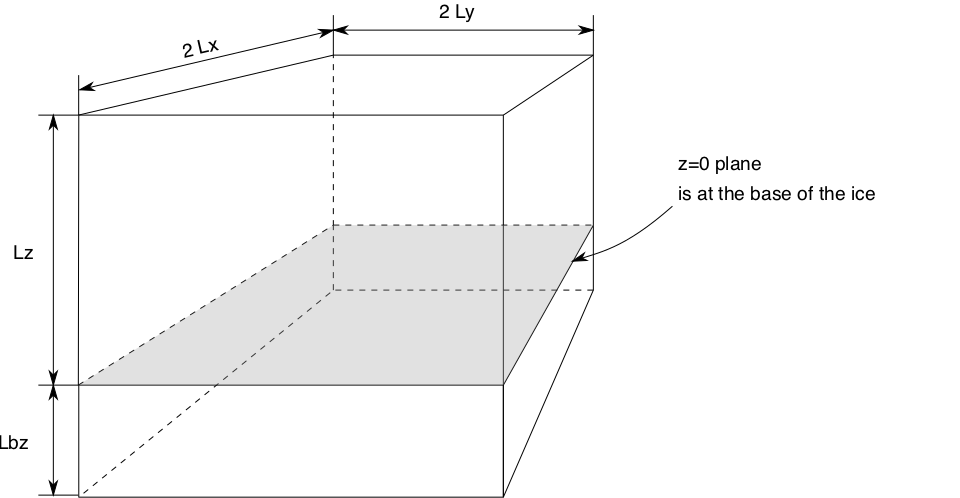
\includegraphics[width=4.0in,keepaspectratio=true]{rectilinearbox}
\caption{PISM's computational box.}
\label{fig:rectilinearbox}
\end{figure}


\subsection{Spatial grid}
\label{subsect:grid}
\optsection{Grid!space}

The PISM grid\index{PISM!grid} covering the computational box is equally spaced in horizontal ($x$ and $y$) directions.  Vertical spacing in the ice is quadratic by default (see below) but optionally a different spacing scheme can be chosen.  (Choose with options \txtopt{z_spacing}{[quadratic, equal]}.) The bedrock thermal layer model always uses equal vertical spacing.

The grid is described by four numbers, namely the number of grid points \texttt{Mx} in the $x$ direction, the number \texttt{My} in the $y$ direction, the number \texttt{Mz} in the $z$ direction within the ice, and the number \texttt{Mbz} in the $z$ direction within the bedrock thermal layer.  These are specified by options \intextoption{Mx}, \intextoption{My}, \intextoption{Mz}, and \intextoption{Mbz}, respectively. The defaults are 61, 61, 31, and 1, respectively.

Note that \texttt{Mx}, \texttt{My}, \texttt{Mz}, and \texttt{Mbz} all indicate the number of grid \emph{points}.  The numbers of grid \emph{spaces} are one less, thus 60, 60, 30, and 0 in the default case.  The lowest grid point in a column of ice, at $z=0$, coincides with the highest grid point in the bedrock, so \texttt{Mbz} must always be at least one and \texttt{Mbz}$>1$ is required to use the bedrock thermal model.  Note that this option is unrelated to the bed deformation model (glacial isostasy model); see option \texttt{-bed_def} (section \ref{subsect:beddef}) for that.

In the quadratic case, the spacing near the ice/bedrock interface is about four times finer than it would be with equal spacing for the same value of \texttt{Mz}, while the spacing near the top is correspondingly coarser. For a detailed description of the spacing of the grid, see the documentation on \texttt{IceGrid::compute_vertical_levels()} in the PISM class browser.

When a thermal bedrock layer is used, the distance \texttt{Lbz} is controlled by the \texttt{-Lbz} option.

If one initializes PISM from a saved model state using \t{-i} then the input model state controls all computational grid parameters.  For instance, the command

\begin{verbatim}
$  pismr -i foo.nc -y 100
\end{verbatim}

\noindent should work fine if \texttt{foo.nc} was a valid PISM model file.  The command

\begin{verbatim}
$  pismr -i foo.nc -Mz 201 -y 100
\end{verbatim}

\noindent will give a warning that ``\texttt{PISM WARNING: ignoring command-line option '-Mz'}'' because \texttt{-i} input files take precedence.

Otherwise, one is allowed to specify the grid when PISM is started.  In particular, the user should specify the grid when using \texttt{-boot_file} or when initializing a simplified-geometry experiment or a verification test, though defaults are generally present in the latter cases.  See sections \ref{sect:start} and \ref{sect:boot} for examples and explanation.


\subsection{Model time}
\label{sec:time}
\optsection{Grid!time}

The following command-line options control PISM time:

\begin{tabular}{lp{0.8\linewidth}}\\
\toprule
\textbf{Option} & \textbf{Meaning}\\
\midrule
\txtopt{y}{(years)} & Number of model years to run.\\
\txtopt{ys}{(years)} & Model year at which to start the run.  Also resets the model time, ignoring any time in the input file.\\
\txtopt{ye}{(years)} & Model year at which to end the run.\\
\bottomrule
\end{tabular}
\\[2em]
\noindent The default value for the end year is the start year (\texttt{-ys} or initialized model time from file) plus the default or given (\texttt{-y}) run length.  If both \texttt{-ys} and \texttt{-ye} are used then the run length is set to the difference.  Using all three of \texttt{-ys}, \texttt{-y} and \texttt{-ys} is not allowed.


\subsection{Diagnostic computations}
\label{sec:diagnostic-computations}

 As a diagnostic example, consider the second of these two runs:
\begin{verbatim}
pisms -y 6000 -o foo.nc
pismr -i foo.nc -y 0 -o bar.nc -o_size big
\end{verbatim}

\noindent The result of this zero-length, ``\texttt{-y 0}'', run is a NetCDF file \texttt{bar.nc} which contains the full three-dimensional velocity field in the scalar NetCDF variables \texttt{uvel}, \texttt{vvel}, and \texttt{wvel}, as well as many other variables.  The file \texttt{foo.nc} does not contain many of these fields because it was written with the default output size of \texttt{medium}.  The ``\texttt{-y 0}'' run has diagnostically ``filled-in'' the fields which PISM can model at a time step, but the model state has not evolved.

In fact, during such a run PISM performs one short time-step to compute ``rates of change'' of ice thickness, surface elevation and other fields, but the model state \emph{is reset} after this step, so re-starting from \texttt{foo.nc} above would give the same result as re-starting from \texttt{bar.nc}.

This diagnostic mode is most frequently associated to the modeling of ice shelves and ice streams.  Subsection \ref{sect:ross} describes using \texttt{pross} to model the Ross ice shelf \cite{MacAyealetal}.  Verification tests I and J, section \ref{sect:verif}, are diagnostic calculations using the SSA.

Note that the NetCDF model state saved by PISM at the end of an \emph{evolution} run does not, by default, contain the three-dimensional velocity field.  Instead, it contains just a bit more than the variables which are needed to restart the run.  One can  force PISM to save all the supported diagnostic quantities at the end of a time-stepping run using the option \texttt{-o_size big}.  Or one can go back and do a ``\texttt{-y 0}'' diagnostic run.


\subsection{Computing ice age} \label{subsect:age}
\optsection{Computing ice age}

By default, PISM does not compute the age of the ice\index{PISM!modeling the age of the ice} because it does not directly impact ice flow when using the default flow laws. It is very easy to turn on.  Just set \intextoption{age}.

  
\subsection{Flotation criterion and mask} \label{subsect:floatmask}  The most basic decision about ice dynamics made internally by PISM is whether to apply the ``flotation criterion'' to determine whether the ice is floating on the ocean or not.  In an evolution run this decision is made at each time step and the result is stored in the \t{mask}.

The possible values of the \t{mask}\index{mask} are given in Table \ref{tab:maskvals}.  The mask does not by itself determine ice dynamics.  For instance, when ice is floating (either value \texttt{MASK_FLOATING} or \texttt{MASK_FLOATING_AT_TIME_0}) the usual choice for ice dynamics is SSA, but the user can choose not to apply that model by not using either option \texttt{-ssa_floating_only} or \texttt{-ssa_sliding}.

\begin{table}[ht]
  \centering
  \caption{The PISM mask\index{mask}, in combination with user options, determines the dynamical model.}\label{tab:maskvals} 
  \small
  \begin{tabular}{p{0.25\linewidth}p{0.65\linewidth}}
    \toprule
    \textbf{Mask value} & \textbf{Meaning}\\\midrule
    1=\texttt{MASK_SHEET} & ice is grounded (and only the SIA is always applied) \\
    2=\texttt{MASK_DRAGGING_SHEET} & ice is grounded (and the SSA is applied if option \texttt{-ssa} is given) \\
    3=\texttt{MASK_FLOATING} & ice is floating (and the SSA is applied if option \texttt{-ssa} is given) \\
    7=\texttt{MASK_FLOATING_AT_TIME_0} & same as \texttt{MASK_FLOATING}, but the grid point was ice free ocean at initialization of the model by \texttt{-boot_file}; ice with this value will calve off if option \texttt{-ocean_kill} is given.
    \\\bottomrule
  \end{tabular}
  \normalsize
\end{table}

Assuming the geometry of the ice evolves (which can be turned off by option \texttt{-no_mass}), and assuming an ocean exists (which can be turned off by option \texttt{-dry}), then at each time step the mask changes by the flotation criterion.  Ice which becomes floating is marked as \texttt{MASK_FLOATING} while ice which becomes grounded is either marked as \texttt{MASK_SHEET} or \texttt{MASK_DRAGGING}.  The latter case occurs if the option \texttt{-ssa_sliding} is used, while otherwise all points are marked \texttt{MASK_SHEET}.


\subsection{Rheology}
\label{sec:rheology}
\optsection{Rheology}

In the polythermal (default) mode of PISM there is only one choice of the flow law: the Glen-Paterson-Budd-Lliboutry-Duval \cite{AschwandenBlatter,LliboutryDuval1985,PatersonBudd}. This law is the only one which we know of in the literature that parameterizes the (observed) softening of pressure-melting-temperature ice, as its liquid fraction increases.

Note that a ``flow law'' here means the function $F(\sigma,T,P,d)$ in the relation
	$$\dot \eps_{ij} = F(\sigma,T,\omega,P,d)\, \sigma_{ij}'$$
where $\dot \eps_{ij}$ is the strain rate tensor, $\sigma_{ij}'$ is the stress deviator tensor, $T$ is the ice temperature, $\omega$ is the liquid water fraction in the ice, $\sigma^2 = \frac{1}{2} \|\sigma_{ij}'\|_F$ so $\sigma$ is the second invariant of the stress deviator tensor, $P$ is the pressure, and $d$ is the grain size.  That is, we are addressing isotropic flow laws only.  In PISM one can choose the scalar function $F$ reasonably arbitrarily by modifying source code,\footnote{See source files \texttt{flowlaws.hh}, \texttt{flowlaws.cc} in \texttt{src/base/rheology/}.} or use the single polythermal law (above), or choose among a number of ``cold ice'' laws listed in table \ref{tab:flowlaw}.

Note that the inverse form of such a flow law in needed for ice shelves and ice streams:
	$$\sigma_{ij}' = 2 \nu(\dot\eps,T,P,d)\,\dot \eps_{ij} $$
Here $\nu(\dot \eps,T,P,d)$ is the effective viscosity.  The need for this inverse form of the flow law explains the ``hybrid'' law \texttt{-ice_type hybrid}, because the inverse form of the Goldsby-Kohlstedt law is unknown.

The command-line option \intextoption{e} sets the flow enhancement factor and can be used with any flow law.  It alters the SIA flow law to be ``$\dot \eps_{ij} = e\, F(\sigma,T,\omega,P,d)\, \sigma_{ij}'.$''

Command-line option \intextoption{ice_type} control the flow law in the \texttt{-cold} mode.  Arguments to \texttt{-ice_type} are in table \ref{tab:flowlaw} below.  One \texttt{-cold} mode ice type, namely \texttt{custom}, is customizable at the command line.\footnote{Run with \texttt{-help} to see all the customizable options for your chosen ice type (since \texttt{-help} displays many options, it is often useful to grep the output, as in \texttt{pisms -ice_type custom -help | grep ice_}).}  One use of the \texttt{custom} ice type is to directly specify the hardness parameter in an ice shelf study.  The viscous stress term in the $x$-component (for example) of the SSA equations for ice shelves and ice streams is
	$$\ddx{}\left(2\nu H\left(2\ddx{u} + \ddy{v}\right)\right)$$
where 
	$$\nu = \frac{\bar B}{2} \left[\left(\ddx{u}\right)^2 + \left(\ddy{v}\right)^2 +
  \frac{1}{4} \left(\ddy{u} + \ddx{v}\right)^2 + \ddx{u}\ddy{v}\right]^{(1-n)/(2n)}.$$
Generally $\bar B$ is computed by a vertical-integral of a function of the temperature field, but it is constant for isothermal ice.  If \intextoption{ice_custom_hardness} is used then $\bar B$ is set to the given value.  The value should have units of Pa $\text{s}^{1/n}$ where $n$ is the Glen exponent (see \texttt{-ice_type}).  Note that the cold-mode ice type (\texttt{-ice_type}) is \texttt{pb} by default, while \intextoption{ice_custom_hardness} is only available when \texttt{-ice_type custom} is given or when the driver has changed the default ice type (in runs such as with \texttt{ssa_testi} and \texttt{pross}).

In the case of \texttt{pross}, which performs the EISMINT Ross ice shelf intercomparison, a constant value $\bar B = 1.9 \times 10^8 \, \text{Pa}\, \text{s}^{1/3}$ is the default \cite{MacAyealetal}.

\begin{table}[ht]
\centering
\caption{\emph{For} \texttt{-cold} \emph{mode only:} Choosing the rheology using \t{-ice_type}.}\label{tab:flowlaw}\index{rheology}\index{flow law}
\small
\begin{tabular}{p{0.15\linewidth}p{0.8\linewidth}}\toprule
\textbf{Type} & \textbf{Comments and Reference} \\ \midrule
\t{pb} &  Paterson-Budd law, the cold-mode default.  Fixed Glen exponent $n=3$.  There is a split ``Arrhenius'' term $A(T) = A \exp(-Q/RT^*)$ where \mbox{$A = 3.615 \times 10^{-13}\, \text{s}^{-1}\, \text{Pa}^{-3}$}, \mbox{$Q = 6.0 \times 10^4\, \text{J}\, \text{mol}^{-1}$} if $T^* < 263$ K and
 \mbox{$A = 1.733 \times 10^{3}\, \text{s}^{-1}\, \text{Pa}^{-3}$}, \mbox{$Q = 13.9 \times 10^4\, \text{J}\, \text{mol}^{-1}$} if $T^* > 263$ K and where $T^*$ is the pressure-adjusted temperature \cite{PatersonBudd}. \\
\t{arr} &  \emph{Cold} part of Paterson-Budd.  Regardless of temperature, the $A$ and $Q$ values for $T^*<263$ K in  the Paterson-Budd law apply.  This is the flow law used in the thermomechanically coupled exact solutions Tests \textbf{F} and \textbf{G} described in \cite{BBL,BB} and run by \texttt{pismv -test F} and \texttt{pismv -test G}. \\
\t{arrwarm} & \emph{Warm} part of Paterson-Budd.  Regardless of temperature, the $A$ and $Q$ values for $T^*>263$ K in Paterson-Budd apply.\\
\t{hooke} & Hooke law.  Fixed Glen exponent $n=3$.  Here  $A(T) = A \exp(-Q/(RT^*) + 3C (T_r - T^*)^\kappa)$; values of  constants as in \cite{Hooke,PayneBaldwin}.\\
\t{hybrid} &  Hybrid of Goldsby-Kohlstedt and Paterson-Budd.  The Goldsby-Kohlstedt law has a combination of exponents  from $n=1.8$ to $n=4$ \cite{GoldsbyKohlstedt}, but in this law it is only used for the SIA, in grounded ice.  The Paterson-Budd law is used for ice streams and ice sheets, that is, the SSA stress balance. \\
\t{custom} & Highly-customizable version of the isothermal Glen flow law.  Allows choice of exponent, hardness/softness parameters, and density. \\
\bottomrule
\normalsize	
\end{tabular}
\end{table}

\begin{comment}
\opt{shelfext\und} When computing ice shelf and stream velocity, PISM enforces boundary conditions using a fictitious extension of the ice shelf over the entire domain.  This extension provides strength only, it does not change the mass, driving force, or location of the calving front.  By default, it's strength will be computed using the current ice type at reference thickness, temperature, and strain rate, customizable using \texttt{-shelfext_H} (5 meters by default), \texttt{-shelfext_T} (263.15 K), \texttt{-shelfext_Du} (1 m/a per km).  The extension strength is used whenever ice thickness is less than the extension thickness to prevent the equations from becoming singular.  You can also specify the extension strength directly using \texttt{-shelfext_force_nuH} with units in Pa s.  Finally, you can compute strength using a \texttt{custom} ice type the ice used in the rest of PISM by giving \texttt{-shelfext_use_private_ice}.  This option will gives you a \texttt{custom} ice type which you can control via \texttt{-shelfext_ice_custom_} (see \texttt{-ice_type}).  All \texttt{-shelfext} options are displayed in \texttt{-help}.
\end{comment}


\subsection{Choosing the stress balance}  \label{subsect:ssacontrol}
\optsection{SSA as a sliding law}

The shallow shelf approximation (SSA)\index{SSA (shallow shelf approximation)} stress balance is used in PISM to describe the sliding of grounded ice and the formation of ice streams \cite{BBssasliding}, as well as being used as the only stress balance for floating ice.  For the SSA with ``plastic'' or ``Coulomb'' till locations of ice streams are determined as part of a free boundary problem identified by Schoof \cite{SchoofStream}.  We believe that this mathematical description of ice streams should be regarded as the best existing ``sliding law'' for the SIA \cite{BBssasliding}.\index{SIA (shallow ice approximation)!sliding laws}

Schoof's model \cite{SchoofStream} describes emergent ice streams within a larger ice sheet and ice shelf system.  It explains the existence of ice streams by a combination of the plastic failure of the till and the SSA approximation of the balance of momentum.  

In PISM the user gives the option \texttt{-ssa_sliding} to turn on the use of the plastic till SSA as a sliding law.  All grounded points are immediately marked as SSA (i.e.~as \texttt{DRAGGING}).  As explained in the next subsection, at these points a yield stress is computed from the amount of stored basal water and from a (generally) spatially-varying till strength, \texttt{tillphi} in an input or output file.  The amount of stored basal water is thermodynamically determined.

\begin{table}[ht]
\centering
\caption{The basic choice of stress balance.}\label{tab:stressbalchoice} 
\small
\begin{tabular}{p{0.25\linewidth}p{0.65\linewidth}}\toprule
\textbf{Option} & \textbf{Semantics}\\ \midrule
    (\emph{NO OPTION}) & Grounded ice flows by the non-sliding SIA.  (Floating ice essentially doesn't flow, so this model is not recommended for marine ice sheets.) \\
    \intextoption{ssa_floating_only} & Only floating ice uses SSA.  Grounded ice marked by mask value \texttt{SHEET} uses the (by default) nonsliding SIA. \\
\intextoption{ssa_sliding} & The recommended default sliding law, which gives the SIA+SSA hybrid stress balance.  Combines SSA-computed velocity, using pseudo-plastic till, with SIA-computed velocity according to the combination in \cite{BBssasliding}.  Floating ice uses SSA only. \\
\bottomrule\end{tabular}
\normalsize
\end{table}

%\intextoption{ice_reg_schoof_length} (1000 km) & Set the ``$L$'' in formula (4.1) in \cite{SchoofStream}.  To use the regularization described by Schoof, one must set \texttt{-ssa_eps 0.0} to turn off the other regularization mechanism, otherwise there is a double regularization (the default except in \texttt{ssa_testi}). \\
%\intextoption{ice_reg_schoof_vel} (1 m/a) & Set the \emph{first} ``$\eps$'' in formula (4.1) in \cite{SchoofStream}.  To deactivate Schoof's regularization, use \texttt{-ice_reg_schoof_vel 0}.  To use the regularization described by Schoof, one must set \texttt{-ssa_eps 0.0} to turn off the other regularization mechanism, otherwise there is a double regularization (the default except in \texttt{ssa_testi}).  Use \texttt{-plastic_reg} above to set the second ``$\eps$'' in formula (4.1) of \cite{SchoofStream}. \\

\begin{table}
  \centering
  \caption{Controlling the SSA stress balance in PISM}
 \begin{tabular}{p{0.2\linewidth}p{0.75\linewidth}}
   \label{tab:ssausage}\\\toprule
   \textbf{Option} & \textbf{Description}\\\midrule
\intextoption{ssa_maxi} (300) & This option sets the maximum allowed number of nonlinear iterations in solving the shallow shelf approximation.  One should usually use option \texttt{-ssa_rtol} to control convergence of the nonlinear iteration.\\
\intextoption{ssa_eps} (1e-15) & The numerical scheme for the shallow shelf approximation  \cite{WeisGreveHutter} computes an effective viscosity which which depends on velocity and temperature.  After that computation, this constant is added to the effective viscosity (to keep it bounded away from zero).  The units are kg $\text{m}^{-1}\,\text{s}^{-1}$.  By default, the regularization in equation (4.1) of \cite{SchoofStream} is also active, use \texttt{-ice_reg_schoof_vel 0} to deactivate Schoof's regularization. Turn off this lower bound mechanise by \texttt{-ssa_eps 0.0} to exclusively use the Schoof regularization mechanism; see \texttt{-ice_reg_schoof_vel} and \texttt{-ice_reg_schoof_length} below.  Note \texttt{-ssa_eps} is set to zero automatically when running \texttt{ssa_testi}. \\
\intextoption{ssa_rtol} (1.0e-4) & The numerical scheme for the shallow shelf approximation \cite{WeisGreveHutter} does a nonlinear iteration wherein velocities (and temperatures) are used to compute a vertically-averaged effective viscosity which is used to solve the equations for horizontal velocity.  Then the new velocities are used to recompute an effective viscosity, and so on.  This option sets the relative change tolerance for the effective viscosity.
In particular, the nonlinear part of the iteration requires that successive values $\nu^{(k)}$ of the vertically-averaged effective viscosity satisfy
	$\frac{\|(\nu^{(k)} - \nu^{(k-1)}) H\|_2}{\|\nu^{(k)} H\|_2} \le \text{ssa_rtol}$
in order to end the iteration with $\nu = \nu^{(k)}$.  See also \texttt{-ksp_rtol}, a PETSc option below, as one may want to require a high relative tolerance for the linear iteration as well.\\
\bottomrule
\end{tabular}
\end{table}


\subsection{Surface gradient method}
\label{subsect:gradient}
\optsection{Driving stress computation}

PISM computes surface gradients to determine the ``driving stress''
	$$(\tau_{d,x},\tau_{d,y}) = - \rho g H \grad h,$$
where $H$ is the ice thickness, and $h = H+b$ is the ice surface elevation.  The driving stress enters into both the SIA and SSA stress balances, but in the former the driving stress is needed on a staggered grid, while in the latter the driving stress is needed on the regular grid.

Surface gradients are computed by finite differences in several slightly-different ways.  There are options for choosing which method to use, but to the best of our knowledge there is no over-arching theoretical advice on the best, most robust mechanism.  There are three methods in PISM, chosen by option \intextoption{gradient}:

\noindent\texttt{-gradient mahaffy}\quad  This most ``standard'' way computes the surface slope onto the staggered grid for the SIA \cite{Mahaffy}.  It makes $O(\Delta x^2,\Delta y^2)$ errors.  For computations of driving stress on the regular grid, centered differencing is used instead.

\noindent\texttt{-gradient haseloff}\quad  This is the default method, but it only differs from the Mahaffy method at ice-margin locations.  It alters the formula for the slope in those cases where an adjacent ice-free bedrock surface elevation is above the ice elevation.  The scheme only differs from \texttt{mahaffy} at such unusual margin points.

\noindent\texttt{-gradient eta}\quad  In this method we first transform the thickness $H$ by $\eta = H^{(2n+2)/n}$ and then differentiate the sum of the thickness and the bed using centered differences:
	$$\grad h = \grad H + \grad b = \frac{n}{(2n+2)} \eta^{(-n-2)/(2n+2)} \nabla \eta + \nabla b.$$
Here $b$ is the bed elevation and $h$ is the surface elevation.  This transformation sometimes has the benefits that the surface values of the horizontal velocity and vertical velocity, and the driving stress, are better behaved near the margin.  See \cite{BLKCB,CDDSV} for technical explanation of this transformation and compare \cite{SaitoMargin}.  The actual finite difference schemes applied to compute the surface slope are similar to option \texttt{mahaffy}.


\subsection{Schoof's parameterization of bed roughness in the SIA} \label{subsect:bedsmooth} \index{Schoof's parameterization of bed roughness}
\optsection{Schoof's parameterization of bed roughness}

Christian Schoof's article \emph{The effect of basal topography on ice sheet dynamics} from 2003 \cite{Schoofbasaltopg2003} describes how to alter the SIA model to more-effectively reproduce ice flow in the vicinity of significant subglacial bedrock topgraphy.  This theory explains that one should use a smoothed (spatially-averaged) bed, but then lower the SIA diffusivity in a precise way in those regions where the significant topography was smoothed-away.  As a practical matter for PISM, this theory improves the SIA model's ability to handle bed roughness because it parameterizes the effects of "higher-order" stresses which act on the ice as it flows over bed topography.   But it also provides a double performance boost, because smoothed beds give longer time steps through the adaptive time-stepping mechanism, \emph{and} because the reduction of diffusivity, which is the parameterized effect of the local bed roughness, gives even longer time-steps.  For a technical description of PISM's implementation of this theory, see the \emph{Browser} page ``Using Schoof's (2003) parameterized bed roughness technique in PISM''.

There is one option which controls this mechanism: \intextoption{bed_smoother_range} gives the half-width of the square smoothing domain in meters.  If zero is given, \texttt{-bed_smoother_range 0} then the mechanism is turned off.  The mechanism is on by default using executable \texttt{pismr}, with the half-width set to 5 km (\texttt{-bed_smoother_range 5.0e3}), giving the recommended smoothing size of 10 km \cite{Schoofbasaltopg2003}.  This mechanism is turned off by default in executables \texttt{pisms} and \texttt{pismv}.

PISM writes fields \texttt{topgsmooth}, \texttt{schoofs_theta}, \texttt{thksmooth} from this mechanism.  (Regarding the last, the thickness is never smoothed, but the thickness relative to the smoothed bedrock elevation, i.e.~the difference between the unsmoothed surface elevation and the smoothed bedrock elevation, is used internally in the mechanism.)


\subsection{Earth deformation models} \label{subsect:beddef} \index{earth deformation} \index{PISM!earth deformation models, using}
\optsection{Earth deformation models}

The option \txtopt{bed_def}{[none, iso, lc]} turns on bed deformation models.

The first model \verb|-bed_def iso|, is instantaneous pointwise isostasy.  This model assumes that the bed at the starting time is in equilibrium with the load.  Then, as the ice geometry evolves, the bed elevation is equal to the starting bed elevation minus a multiple of the increase in ice thickness from the starting time: $b(t,x,y) = b(0,x,y) - f [H(t,x,y) - H(0,x,y)]$.  Here $f$ is the density of ice divided by the density of the mantle, so its value is determined by setting the values of \verb|lithosphere_density| and \verb|ice_density| in the configuration file; see subsection \ref{sec:pism-defaults}.  For an example and verification, see Test H in Verification section. 

The second model \verb|-bed_def lc| is much more effective.  It is based on papers by Lingle and Clark \cite{LingleClark}\index{People!Lingle, Craig} \index{People!Clark, J.} and Bueler and others \cite{BLKfastearth}.  It generalizes and improves the most widely-used earth deformation model in ice sheet modeling, the flat earth Elastic Lithosphere Relaxing Asthenosphere (ELRA) model \cite{Greve2001}.  It imposes  essentially no computational burden because the Fast Fourier Transform is used to solve the linear differential equation \cite{BLKfastearth}.  When using this model in PISM, the rate of bed movement (uplift) is stored in the PISM output file and then is used to initialize the next part of the run.  In fact, if gridded ``observed'' uplift data is available, for instance from a combination of actual point observations and/or paleo ice load modeling, and it that uplift field is put in a NetCDF variable with standard name \verb|tendency_of_bedrock_altitude| in the  \texttt{-boot_file} file, then this model will initialize so that it starts with the given uplift rate.

Minimal example runs to compare these models:
\begin{verbatim}
$ mpiexec -n 4 pisms -eisII A -y 8000 -o eisIIA_nobd.nc
$ mpiexec -n 4 pisms -eisII A -bed_def iso -y 8000 -o eisIIA_bdiso.nc
$ mpiexec -n 4 pisms -eisII A -bed_def lc -y 8000 -o eisIIA_bdlc.nc
\end{verbatim}
Compare the \texttt{topg}, \texttt{usurf}, and \texttt{dbdt} variables in the resulting output files.

Test H in section \ref{sect:verif} can be used to reproduce the comparison done in \cite{BLKfastearth}.

\subsection{Disabling PISM components}
\label{sec:turning-off}
\optsection{Disabling PISM components}

Major model components, unlike ``peripheral'' ones like bed deformation, do not need to be turned ``on'' explicitly.\footnote{It would be a hassle to ask for SIA computations every time you need them, for example.} However, in some cases it is useful to be able to disable particular components (during model spin-up, for example). Currently PISM has switches disabling the mass-continuity step (command-line option \intextoption{no_mass}), energy balance computation (option \intextoption{no_energy}) and polythermal energy balance computation: option \intextoption{cold} makes PISM use temperature instead of enthalpy in the energy balance code.

%%% Local Variables: 
%%% mode: latex
%%% TeX-master: "manual"
%%% End: 

% LocalWords:  intercomparison PDD polythermal Lliboutry Duval


\clearpage\newpage

\section{Making \emph{HARD} Modeling Choices}
\label{sec:hard-choices}

Most uses of an ice sheet model depend on careful modeling choices in situations where there are considerable uncertainties \emph{and} the model results depend strongly on those choices.  There may be, at the present state of knowledge, \emph{no clear default values} that PISM can provide.

The current section collects some modeling choices which have this ``hard'' flavor.  The available PISM options related to these choices are known to be \emph{not} sufficient for all users.  These are modeling choices for which \emph{we know} the user may have to do a great deal more hard work than just choose among PISM runtime options.  Here are real example cases where users have worked hard:
\begin{itemize}
\item User was required to make use of available data in order to choose parameters for existing PISM models.  These parameters will then override PISM defaults:
\begin{center} % our UAF current situation with Greenland
\fbox{ \begin{minipage}[t]{5.0in}
\emph{Example}.  Use regional atmosphere model output to identify PDD parameters suitable for modeling surface mass balance on a particular ice sheet.  Then supply these parameters to PISM by a \texttt{-config\_override} file.
\end{minipage} }
\end{center}
\item User was required to write code, including code which modified current PISM internals, either to add additional processes or to ``correct'' PISM default process models; or 
\begin{center} % e.g. harder case is Potsdam marine ice sheet mods
\fbox{ \begin{minipage}[t]{5.0in}
\emph{Example}.  Add a new sub-ice-shelf melt model by modifying C++ code in the \texttt{src/coupler/} directory.
\end{minipage} }
\end{center}
\item User deliberately simplified the model in use, instead of the default which was ``throwing in the kitchen sink''.
\begin{center} % Nick's -hold_tauc choice
\fbox{ \begin{minipage}[t]{5.0in}
\emph{Example}.  Instead of using the PISM default mechanism connecting basal melt rate and basal strength, bypass this mechanism and impose a map of yield stress \texttt{tauc} directly.
\end{minipage} }
\end{center}
\end{itemize}

Obviously there is no actual clear distinction between the ``hard'' choices in this section and the ``easy'' ones in the previous section, but the subsections here cover issues for which the PISM developers have a hard time supplying easy answers!

\subsection{Setting up PISM boundary (atmosphere, surface and ocean) models}
\label{sec:boundary-models}

Setting up PISM's boundary models requires selecting one model of each kind\footnote{Using a default model is a choice.} and zero or more ``model modifiers''.  The selected models and modifiers are chained as in Figure~\ref{fig:climate-input-data-flow} on page \pageref{fig:climate-input-data-flow}.

Command-line options \texttt{-atmosphere}, \texttt{-surface} and \texttt{-ocean} each take a comma-separated list of keywords as an argument; the first keyword \emph{has} to correspond to a model, the rest can be modifiers. Any of these options can be omitted to use the default atmosphere, surface or ocean model, although using a modifier requires specifying a model.

For example,
\begin{verbatim}
$ pismr -i foo.nc -atmosphere searise_greenland,dTforcing \
        -dTforcing delta_T.nc -surface pdd
\end{verbatim}%$
chooses a combination of the SeaRISE-Greenland atmosphere model (see below), modified by an ice-core-derived paleo-temperature forcing (shift), and a positive degree-day (PDD) local surface mass balance model.  Because it is not mentioned, the ocean model is the default one (\texttt{-ocean constant}).

Atmosphere and surface models have two ``modifiers'' available; the corresponding keywords are \texttt{forcing} and \texttt{lapse_rate}. The ocean model supports the \texttt{forcing} modifier only. Please see below for details.

\subsubsection{PISM atmosphere models}
\label{sec:pism-atmosphere}
\optsection{Climate (boundary) models!\texttt{-atmosphere} [searise_greenland, constant, given, lapse_rate, forcing]}

\begin{itemize}
  \item \emph{SeaRISE-Greenland} (\texttt{searise_greenland}, the default)

    This atmosphere model implements a longitude, latitude and elevation dependent near-surface air temperature parameterization and a cosine yearly cycle described in \cite{Faustoetal2009} and uses a constant in time ice-equivalent precipitation field (in units of thickness per time, variable \texttt{precip}) that is read from an input file.  The air temperature parameterization is controlled by configuration parameters with the \texttt{snow_temp_fausto} prefix.

    In addition to the temperature parameterization it allows using the SeaRISE-Greenland formula for paleo-precipitation correction from present; a 7.3\% change of precipitation rate for every one degree Celsius of temperature change \cite{Huybrechts02}.  See \url{http://websrv.cs.umt.edu/isis/index.php/Model_Initialization#Greenland} for details.  Turn on this mechanism by using the \intextoption{paleo_precip} option.

    It expects variables \texttt{precip}, latitude and longitude to be present in an input file.

 \item \emph{Constant in time} (\texttt{constant})

    This atmosphere model reads the snow precipitation (variable \texttt{precip}) and the mean annual near-surface air temperature (variable \texttt{artm}) and provides them to a surface model.

  \item \emph{Reading atmosphere boundary conditions from a file} (\texttt{given})

    This atmosphere model is similar to \texttt{constant} in that it uses \texttt{artm} and \texttt{precip} fields given by the user by providing them directly to the surface model. The name of the file PISM will read \texttt{artm} and \texttt{precip} from is specified using the \fileopt{bc_file} option.

    A file \texttt{foo.nc} used with \texttt{-atmosphere given -bc_file foo.nc} should contain several records;\footnote{If this file contains one record (i.e. fields corresponding to one time value only), \texttt{-atmosphere given} is essentially equivalent to \texttt{-atmosphere constant}.} the time variable (\texttt{'t'}) should describe what model time these records correspond to.

    This model was created to force PISM with sampled (possibly periodic) climate data, e.g. using monthly records of \texttt{artm} and \texttt{precip}.

  \end{itemize}

  Currently there are two ``modifiers'' one can use with an atmosphere model.

  The atmosphere \texttt{dTforcing} modifier implements temperature forcing using scalar offsets and \texttt{anomaly} modifier a mechanism applying precipitation and temperature anomalies.
  \begin{itemize}
  \item \fileopt{dTforcing} specifies a file containing scalar temperature offsets (for use with \texttt{dTforcing}, variable \texttt{delta_T}), 
  \item \fileopt{anomaly_temp} specifies a file containing spatially-variable near-surface air temperature anomalies (variable \texttt{temp_anomaly}), and
  \item \fileopt{anomaly_precip} specifies a file containing spatially-variable ice-equivalent precipitation anomalies (in units of thickness per time, variable \texttt{precip_anomaly}).
  \end{itemize}

  Options \texttt{-anomaly_temp} and \texttt{-anomaly_precip} can be used to set up a PISM run using a GCM output, essentially achieving one-way coupling. See also the \texttt{-surface given} option, below.

 The \texttt{lapse_rate} modifier allows correcting air temperature and precipitation using elevation lapse rates. It uses the following options.
  \begin{itemize}
  \item \fileopt{bc_file} specifies the file containing the reference surface elevation field (standard name: \texttt{surface_altitude}). This file can contain several surface elevation records to use lapse rate corrections relative to time-dependent surface. If one record is provided, the reference surface elevation is assumed to be time-independent.
  \item \intextoption{bc_period} gives the period, in model years, to use when interpreting data in the file given with \texttt{-bc_file},
  \item \intextoption{bc_reference_year} takes the time $T$ in model years. The record for $t$ years in \texttt{-bc_file} is interpreted as corresponding to $t$ years since $T$.
  \item \intextoption{bc_time_average} enables interpolating (and in some cases, averaging) B.C. data in time.
  \item \intextoption{temp_lapse_rate} gives the temperature lapse rate, in $K/km$. Note that we use the following definition of the temperature lapse rate:
    \begin{displaymath}
      \gamma = -\frac{dT}{dz}.
    \end{displaymath}
  \item \intextoption{precip_lapse_rate} gives the precipitation lapse rate, in $m/year/km$. Here $\gamma = -\frac{dM}{dz}$.
  \end{itemize}

\subsubsection{PISM surface mass and energy process models}
\label{sec:pism-surface-snow}
\optsection{Climate (boundary) models!\texttt{-surface} [simple, constant, elevation, given, pdd, forcing]}

\begin{itemize}
  \item \emph{The ``invisible'' model} (\texttt{simple}, the default)

    This is the simplest ``surface model'' available in PISM.  Its job is to re-interpret  precipitation as surface mass flux (balance), and to re-interprets mean annual near-surface (2m) air temperature as the temperature of the ice at the depth at which firn processes cease to change the temperature of the ice.  (I.e.~the temperature \emph{below} the firn.)  This implies that there is no melt.  Though primitive, this model may be desired in cold environments (e.g.~East Antarctic ice sheet) in which melt is negligible and heat from firn processes is ignored.

  \item \emph{Constant in time} (\texttt{constant})

    This surface model reads constant in time ice upper surface boundary conditions from a file.  These fields are provided directly to the ice dynamics model (see table \ref{tab:ice-dynamics-bc}).  Variables \texttt{artm} (ice temperature at the ice surface but below firn) and \texttt{acab} (top surface mass flux into the ice) are read from the file, so this choice will cause PISM to stop if they are not present in the input file.

    Note: this surface model \emph{ignores} the atmosphere model selection made using the \texttt{-atmosphere} option.

  \item \emph{Reading top-surface boundary conditions from a file} (\texttt{given})

    This surface model is similar to \texttt{constant} in that it uses \texttt{artm} and \texttt{acab} fields given by the user by providing them directly to the ice dynamics model. The name of the file PISM will read \texttt{artm} and \texttt{acab} from is specified using the \fileopt{bc_file} option.

    A file \texttt{foo.nc} used with \texttt{-surface given -bc_file foo.nc} should contain several records;\footnote{If this file contains one record (i.e. fields corresponding to one time value only), \texttt{-surface given} is essentially equivalent to \texttt{-surface constant}.} the time variable (\texttt{'t'}) should describe what model time these records correspond to.

    This model was created to force PISM with sampled (possibly periodic) climate data, e.g. using monthly records of \texttt{artm} and \texttt{acab}.

 Option \txtopt{bc_artm_lapse_rate}{Kelvin per kilometer} corrects \texttt{artm} with respect to a reference surface \texttt{usurf} using a lapse rate. \texttt{usurf} must be present in \texttt{foo.nc}.

 Option \txtopt{bc_acab_lapse_rate}{meters per year per kilometer} corrects \texttt{acab} with respect to a reference surface \texttt{usurf} using a lapse rate following [\href{http://www.truenuff.tv/glacierrace.php}{86}]. \texttt{usurf} must be present in \texttt{foo.nc}.

Option \txtopt{bc_period}{years} makes PISM interpret data in \texttt{-bc_file} as periodic. In this case the time in the NetCDF file is understood as the time \emph{from the beginning of a period}, i.e. from the beginning of a year with \texttt{-bc_period 1}, from the beginning of a decade with \texttt{-bc_period 10}, etc.

For example, to use monthly records and period of 1 year, create a file (say, ``\texttt{foo.nc}'') with 12 records. The variable \texttt{'t'} should contain 0, 1, 2, 3, \dots, 11 and have the units of ``month'' (you can use other units, too). Then, run
\begin{verbatim}
$ pimsr -surface given -bc_file foo.nc -bc_period 1
\end{verbatim}%$

To force PISM using monthly records with longer periods, just add more records to the \texttt{-bc_file}  and change the \texttt{-bc_period} value.

\noindent Notes:
\begin{itemize}
\item PISM can handle files with virtually any number of records: it will
  read and store in memory at most \texttt{climate_forcing_buffer_size} records
  at any given time (default: 60, or 5 years' worth of monthly fields).
\item this surface model \emph{ignores} the atmosphere model selection made
  using the \texttt{-atmosphere} option,
\item when preparing a file for use with this model, it is best to use the \texttt{t,x,y} variable storage order: files using this order can be read in faster than ones using the \texttt{t,y,x} order, for reasons explained in section \ref{sec:pism-io-performance}.

To change the storage order in a NetCDF file, use \texttt{ncpdq}:
\begin{verbatim}
$ ncpdq -a t,x,y input.nc output.nc
\end{verbatim}%$
will copy data from \texttt{input.nc} into \texttt{output.nc}, changing the storage order to \texttt{t,x,y} at the same time.
\end{itemize}

  \item \emph{Elevation-dependent temperature and mass balance} (\texttt{elevation})

   This surface model parametrizes the ice surface temperature $T_{h}$ = \texttt{artm} and the surface mass balance $m$ = \texttt{acab} as a \emph{piecewise-linear} function of surface elevation $h$.

    The option \txtopt{artm}{\emph{list of 4 numbers}} determines the surface temperature using the 4 parameters $T_{\mathrm{min}}$, $T_{\mathrm{max}}$, $h_{\mathrm{min}}$, $h_{\mathrm{max}}$. Let
    \begin{equation}
      \mathrm{d}T/\mathrm{d}h = (T_{\text{max}} - T_{\text{min}}) / (h_{\text{max}} - h_{\text{min}})
    \end{equation}
    be the temperature gradient.  Then
    \begin{equation}
      T(x,y) = \begin{cases}
        T_{\text{min}}, & h(x,y) \le h_{\text{min}}, \\
        T_{\text{min}} + \mathrm{d}T/\mathrm{d}h\,(h(x,y) - h_{\text{min}}),
        &  h_{\text{min}} < h(x,y) < h_{\text{max}}, \\
        T_{\text{max}}, & h_{\text{max}} \le h(x,y). \end{cases}
    \end{equation}
    
    The option \txtopt{acab}{\emph{list of 5 numbers}} determines the surface mass balance using the 5 parameters $m_{\mathrm{min}}$, $m_{\mathrm{max}}$, $h_{\mathrm{min}}$, $h_{\mathrm{ELA}}$, $h_{\mathrm{max}}$. Let
    \begin{equation}
      \mathrm{d}m_{\mathrm{abl}}/\mathrm{d}h = - m_{\text{min}} / (h_{\text{max}} - h_{\text{min}})
    \end{equation}
    and
    \begin{equation}
      \mathrm{d}m_{\mathrm{acl}}/\mathrm{d}h = m_{\text{max}} / (h_{\text{max}} - h_{\text{min}})
    \end{equation}
    be the mass balance gradient in the ablation and in the accumulation area, respectively.  Then
    \begin{equation}
      m(x,y) = \begin{cases}
        m_{\text{min}}, & h(x,y) \le h_{\text{min}}, \\
        \mathrm{d}m_{\mathrm{abl}}/\mathrm{d}h\,(h(x,y) - h_{\text{ELA}}),
        &  h_{\text{min}} < h(x,y) < h_{\text{max}}, \\
        \mathrm{d}m_{\mathrm{acl}}/\mathrm{d}h\,(h(x,y) - h_{\text{ELA}}),
        &  h_{\text{min}} < h(x,y) < h_{\text{max}}, \\
        m_{\text{max}}, & h_{\text{max}} \le h(x,y). \end{cases}
    \end{equation}
    The option \txtopt{acab_limits}{\emph{list of 2 numbers}} limits the mass balance below $h_{\mathrm{min}}$ to $m^{*}_{\mathrm{min}}$ and above $h_{\mathrm{max}}$ to $m^{*}_{\mathrm{max}}$, thus
    \begin{equation}
      m(x,y) = \begin{cases}
        m^{*}_{\text{min}}, & h(x,y) \le h_{\text{min}}, \\
        \mathrm{d}m_{\mathrm{abl}}/\mathrm{d}h\,(h(x,y) - h_{\text{ELA}}),
        &  h_{\text{min}} < h(x,y) < h_{\text{max}}, \\
        \mathrm{d}m_{\mathrm{acl}}/\mathrm{d}h\,(h(x,y) - h_{\text{ELA}}),
        &  h_{\text{min}} < h(x,y) < h_{\text{max}}, \\
        m^{*}_{\text{max}}, & h_{\text{max}} \le h(x,y). \end{cases}
    \end{equation}

    Note: this surface model \emph{ignores} the atmosphere model selection made using the \texttt{-atmosphere} option.

 \item \emph{Temperature-index (positive degree-day) scheme} (\texttt{pdd}) \index{temperature-index surface processes model} \index{positive degree day surface processes model} \index{PDD (positive degree day model)} \index{PISM!default positive degree day model} 

   The default PDD used by PISM, turned on by option \texttt{-surface pdd}, is based on \cite{CalovGreve05} and EISMINT-Greenland intercomparison (section \ref{sec:eismint-greenland} and \cite{RitzEISMINT}).  It also implements latitude- and mean July temperature dependent ice and snow factors using formulas in \cite{Faustoetal2009}.

   Our PDD implementation is meant to be used with an atmosphere model implementing a cosine yearly cycle such as \texttt{searise_greenland}, but is not restricted to parameterizations like this one. A PDD generally adds ``white noise'' to the seasonal cycle to simulate additional daily variability associated to the vagaries of weather.  This additional random variation is quite significant, as the seasonal cycle may never reach the melting point but that point may be reached with some probability, in the presence of the daily variability, and thus melt may occur.  Concretely, a normally-distributed, mean zero random temperature increment is added to the seasonal cycle.  The standard deviation of the daily variability is controlled by the \intextoption{pdd_std_dev} option (and the corresponding config. parameter), and defaults to 2.53 degrees \cite{Faustoetal2009}. There is no assumed spatial correlation of daily variability.

The number of positive degree days is computed as the magnitude of the temperature excursion above $0\!\phantom{|}^\circ \text{C}$ multiplied by the duration (in days) when it is above zero.  In PISM there are actually two methods for computing the number of positive degree days.  The first computes only the expected value, by the method described in \cite{CalovGreve05}.  This is the default when a PDD is chosen (i.e.~option \texttt{-surface pdd}).  The second is a monte carlo simulation of the white noise itself, chosen by adding the option \intextoption{pdd_rand}.  This monte carlo simulation adds the same daily variation at every point, though the seasonal cycle is (generally) location dependent.  If repeatable randomness is desired use \intextoption{pdd_rand_repeatable} instead of \texttt{-pdd_rand}.

The number of positive degree days is multiplied by a coefficient (config parameter \texttt{pdd_factor_snow}) to compute the amount of snow melted.  Of the melted snow, a fraction (\texttt{pdd_refreeze}) is kept as ice.  This ice, plus all unmelted snow (already measured as ice-equivalent) is added to the mass balance, unless the number of positive degree days exceeds that required to melt all of the snow.  In this latter case, in which there are excess positive degree days available for melting, the excess is multiplied by a coefficient (\texttt{pdd_factor_ice}) to compute how much ice is melted.  In this case actual ablation occurs at that location.

In addition to this, one can use latitude- and July-air-temperature-dependent Greenland PDD model parameters $\beta_{\mathrm{ice}}$ and $\beta_{\mathrm{snow}}$ (formulas (6) and (7) in \cite{Faustoetal2009}) by adding the \intextoption{pdd_fausto}  option. See also configuration parameters with the \texttt{pdd_fausto} prefix.

\end{itemize}

The \texttt{dTforcing} modifier implements temperature forcing using scalar offsets and uses the \texttt{-dTforcing} option. This modifier is identical to the corresponding atmosphere modifier, but applies offsets at a different stage in the computation of top-surface boundary conditions needed by the ice dynamics core.

The \texttt{forcing} modifier implements a surface mass balance adjustment mechanism which forces ice thickness to a target thickness distribution at the end of the run.  The idea behind this mechanism is that spinup of ice sheet models frequently requires the surface elevation to come close to measured values at the end of a run.  A simpler alternative to accomplish this, namely option \intextoption{no_mass}, represents an unmodeled, frequently large, violation of the mass continuity equation.

In more detail, let $H_{\text{tar}}$ be the target thickness.  Let $H$ be the time-dependent model thickness.  Note that a surface model as described in this section produces the $M$ term in the mass continuity equation
  $$\frac{\partial H}{\partial t} = M - S - \nabla\cdot \mathbf{q}.$$
(Other details of this equation do not concern us here.)  Option \fileopt{force_to_thk} causes $M$ to be modified by a multiple of the difference between the target thickness and the current thickness,
  $$\Delta M = \alpha (H_{\text{tar}} - H)$$
where $\alpha>0$.  We are adding mass ($\Delta M>0$) where $H_{\text{tar}} > H$ and ablating where $H_{\text{tar}} < H$.  We make this mechanism stronger as the run goes on, as follows: if $t_s$ be the start time and $t_e$ the end time for the run then $\alpha=\alpha(t)$ where $\alpha(t) = \alpha_0 (t-t_s)/(t_e-t_s)$.

Option \fileopt{force_to_thk} identifies the file containing the target ice thickness field.  A basic run modifying surface model \texttt{constant} would look like
\begin{verbatim}
$ pismr -i foo.nc -surface constant,forcing -force_to_thk bar.nc
\end{verbatim}%$
In this case \texttt{foo.nc} contains fields \texttt{acab} and \texttt{artm}, as normal for \texttt{-surface constant}, and \texttt{bar.nc} contains field \texttt{thk} which will serve as the target thickness.  Option \intextoption{force_to_thk_alpha} adjusts the value of $\alpha_0$, which has a default value specified in the \emph{Source Code Browser} \url{\PISMBROWSERURL}.

  The \texttt{lapse_rate} modifier allows correcting ice-surface temperature and surface mass balance using elevation lapse rates. It uses the following options.
  \begin{itemize}
  \item \fileopt{bc_file} specifies the file containing the reference surface elevation field (standard name: \texttt{surface_altitude}). This file can contain several surface elevation records to use lapse rate corrections relative to time-dependent surface. If one record is provided, the reference surface elevation is assumed to be time-independent.
  \item \intextoption{bc_period} gives the period, in model years, to use when interpreting data in the file given with \texttt{-bc_file},
  \item \intextoption{bc_reference_year} takes the time $T$ in model years. The record for $t$ years in \texttt{-bc_file} is interpreted as corresponding to $t$ years since $T$.
  \item \intextoption{bc_time_average} enables interpolating (and in some cases, averaging) B.C. data in time.
  \item \intextoption{temp_lapse_rate} gives the temperature lapse rate, in $K/km$. Note that we use the following definition of the temperature lapse rate:
    \begin{displaymath}
      \gamma = -\frac{dT}{dz}.
    \end{displaymath}
  \item \intextoption{smb_lapse_rate} gives the surface mass balance lapse rate, in $m/year/km$. Here, $\gamma=-\frac{dM}{dz}$.
  \end{itemize}


\subsubsection{PISM ocean models}
\label{sec:pism-ocean-models}
\optsection{Climate (boundary) models!\texttt{-ocean} [constant, forcing]}

PISM includes one simple ocean model: \texttt{constant}, providing constant (both in time and space) mass flux into the ocean and sea level elevation to PISM's ice flow core. The mass flux is controlled by the\\ \texttt{ocean_sub_shelf_heat_flux_into_ice} configuration parameter and the assumption that the mass flux is proportional to heat flux into ice.

  The ocean \texttt{dSLforcing} modifier implements sea level forcing. The command-line option \fileopt{dSLforcing} is used to specify the file containing sea level offsets:
\begin{verbatim}
$ pismr -i in.nc -ocean constant,dSLforcing -dSLforcing delta_SL.nc
\end{verbatim}%$
uses \texttt{delta_SL.nc}

\subsection{Controlling basal strength}  \label{subsect:basestrength}
\optsection{Basal strength and sliding}

In the \t{-ssa_sliding} case of a SIA+SSA hybrid model, the determination of basal resistance comes in part from a stored basal till material property $\phi=$\texttt{tillphi}, the till friction angle \cite{Paterson}.  The actual strength value is a till yield stress $\tau_c$, which necessarily represents the strength of the aggregate material at the base of an ice sheet, a poorly observed mixture of liquid water, ice, and granular till.  The value of $\tau_c$ is determined in part by a basal water model and in part by $\phi$, using a Mohr-Coulomb criterion \cite[Chapter 8]{Paterson}, 
\begin{equation*}
   \tau_c = c_{0} + (\tan\phi)\,(\rho g H - p_w).
\end{equation*}
Here $H$ is the ice thickness, $\rho$ the ice density, $g$ the acceleration of gravity, $p_w$ is the modeled pore water pressure, and $\phi$ is the till friction angle.  The difference $(\rho g H - p_w)$ is the modeled value of the effective pressure on the material till.  Note Schoof \cite{SchoofStream} formula (2.4) uses till cohesion $c_0 = 0$ and that is the default value in PISM.

\begin{table}
  \centering
  \caption{Basal strength command-line options}
  \begin{tabular}{lp{0.6\linewidth}}
    \\\toprule
    \textbf{Option} & \textbf{Description}
    \\\midrule
    \txtopt{topg_to_phi}{\emph{list of 5 numbers}} & Compute $\phi$ using \eqref{eq:1} and \eqref{eq:2}.\\
    \txtopt{plastic_pwfrac}{\emph{pure number}} & Set what fraction of overburden pressure is assumed as the till pore water pressure.  Only relevant at basal points where there is a positive amount of basal water.\\
    \intextoption{plastic_c0} & Set the value of the till cohesion ($c_{0}$) in the plastic till model.  The value is a pressure, given in kPa.\\
    \txtopt{plastic_reg}{(m/a)} & Set the value of $\eps$ regularization of plastic till; this is the second ``$\eps$'' in formula (4.1) in \cite{SchoofStream}. The default is $0.01$.\\
    \txtopt{plastic_phi}{(degrees)} & Use a constant till friction angle. The default is $30^{\circ}$.\\
    \intextoption{pseudo_plastic_q} & Set the exponent $q$.\\
    \txtopt{pseudo_plastic_uthreshold}{(m/a)} & Set $u_{\text{threshold}}$. The default is $100$ m/a.\\
    \intextoption{hold_tauc} &   Keep the current values of the till yield stress $\tau_c$.  That is, do not update them by the default model using the stored basal melt water.  Only effective if \texttt{-ssa_sliding} is also set.
   \\\bottomrule
  \end{tabular}
 \label{tab:basal-strength}
\end{table}

Option \texttt{-plastic_pwfrac} determines $\alpha$, the quantity controlling how $p_w$ is determined from the effective thickness of basal water, the quantity $w=$\texttt{bwat}.  The formula is $p_w = \alpha\, w \rho g H$.  See \cite{BKAJS}.

We find that an effective, though heuristic, way to determine \texttt{tillphi} is to make it a function of bed elevation \cite{BKAJS}.  This heuristic is motivated by hypothesis that basal material with a marine history should be weak \cite{HuybrechtsdeWolde}.

Thus PISM has a mechanism setting $\phi$=\texttt{tillphi} to a \emph{piecewise-linear} function of bed elevation.  Given 5 parameters: $\phi_{\mathrm{min}}$, $\phi_{\mathrm{max}}$, $b_{\mathrm{min}}$, $b_{\mathrm{max}}$, $\phi_{\mathrm{ocean}}$, where $b$ stands for the bed elevation, let 
\begin{equation}
  M = (\phi_{\text{max}} - \phi_{\text{min}}) / (b_{\text{max}} - b_{\text{min}})\label{eq:1}
\end{equation}
be the slope of the nontrivial part.  Then
\begin{equation}
  \phi(x,y) = \begin{cases}
    \phi_{\text{min}}, & b(x,y) \le b_{\text{min}}, \\
    \phi_{\text{min}} + (b(x,y) - b_{\text{min}}) \,M,
    &  b_{\text{min}} < b(x,y) < b_{\text{max}}, \\
    \phi_{\text{max}}, & b_{\text{max}} \le b(x,y). \end{cases}\label{eq:2}
\end{equation}
The exception is if the point is marked as floating, in which case the till friction angle
is set to the value $\phi_{\mathrm{ocean}}$.

Actually the ``yield stress'' $\tau_c$ can be part of a power law model.  In fact, the basal resistance is normally determined by a user-configurable ``pseudo-plastic'' power law.  Specifically, stress is generally a power law function of basal sliding velocity $\mathbf{u}$:
   $$\tau_b = \tau_c \frac{|\mathbf{u}|^{q-1}}{u_{\text{threshold}}^q}\, \mathbf{u}.$$
Here $\tau_c$ corresponds to the variable \texttt{tauc} in PISM input and output files, $q$ is the power controlled by \texttt{-pseudo_plastic_q}, and the threshold velocity $u_{\text{threshold}}$ is controlled by \texttt{-pseudo_plastic_uthreshold}.  The purely plastic case is $q=0$---see \cite{SchoofStream} for precise interpretation---and the linear case is $q=1$, in which case the coefficient of velocity, $\tau_c/u_{\text{threshold}}$, is more commonly called $\beta$ or $\beta^2$ \cite{MacAyeal}.

See \emph{PISM Source Code browser}, source file \texttt{iMbasal.cc}, and \cite{BBssasliding,BKAJS} for more details.

The major example of \texttt{-ssa_sliding} usage is in the first section of this manual.  A made-up example, in which sliding happens in the ``trough'', is
\begin{verbatim}
pisms -eisII I -ssa_sliding -track_Hmelt -Mx 91 -My 91 -Mz 51 \
      -topg_to_phi 5.0,15.0,0.0,1000.0 -y 12000
\end{verbatim}

A final note on basal sliding is in order.  There can be sliding in the SIA stress balance model (paradigm) itself, where the velocity of sliding is a direct function of the driving stress.  Such a SIA sliding mechanism appears in ISMIP-HEINO \cite{Calovetal2009HEINOfinal} and many other SIA-based modeling efforts in the literature.  \emph{This kind of sliding is not recommended, as it does not make sense to regard the driving stress as the local generator of flow if the bed is not holding all of that stress.}  Within PISM there is an implementation of SIA-based sliding for the verification test E, see \texttt{SIA_Sliding.cc}.  PISM does \emph{not} support this sliding mode in other contexts.  

% undocumented options/config. parameters
% base/iMoptions.cc:  "thk_eff" : "thk_eff_basal_water_pressure"
% base/iMoptions.cc:  "thk_eff_H_high" : "thk_eff_H_high"
% base/iMoptions.cc:  "thk_eff_H_low" : "thk_eff_H_low"
% base/iMoptions.cc:  "thk_eff_reduced" : "thk_eff_reduced"
% base/iMoptions.cc:  "bmr_enhance" : "bmr_enhance_basal_water_pressure"
% base/iMoptions.cc:  "bmr_enhance_scale" : "bmr_enhance_scale"


%%% Local Variables: 
%%% mode: latex
%%% TeX-master: "manual"
%%% End: 

% LocalWords:  PDD pdd html PISM PISM's paleo


\clearpage\newpage


\section{PISM-PIK improvements for marine ice sheet modeling}
\label{sec:pism-pik}
\index{PISM!PISM-PIK}
\optsection{PISM-PIK}

References \cite{Albrechtetal2011} and \cite{Winkelmannetal2010TCD} describe improvements to the grounded, SSA-as-a-sliding law model of \cite{BBssasliding}.  These improvements make PISM an effective Antarctic model, as demonstrated by \cite{Martinetal2010TCD,Levermann2011}.  Because these improvements had a separate existence as the PISM-PIK model from 2009--2010, we call them the ``\emph{PISM-PIK improvements}'' here.

These model improvements all relate to the stress balance and geometry changes that apply at the vertical calving face of floating ice shelves.  The physics at such calving fronts is very different from elsewhere on an ice sheet, because the flow is nothing like the lubrication flow addressed by the SIA, and nor is the physics like the sliding flow in the interior of an ice domain, where sliding alters geometry according to the basic mass continuity equation.  The correct physics at the calving front can be thought of as certain modifications to the mass continuity equation and to the SSA stress balance equation.  The code implementing the PISM-PIK improvements makes these highly-nontrivial modifications of the finite difference/volume equations in PISM.

\subsection{Partially-filled cells at the boundaries of ice shelves}
\label{sec:part-grid}

Albrecht et al \cite{Albrechtetal2011} argue that the correct movement of the ice shelf calving front on a finite-difference grid, assuming for the moment that ice velocities are correctly determined (see below), requires tracking some cells as being partially-filled (option \intextoption{part_grid}). If the calving front is moving forward, for example, it is not correct to add a little mass to the next cell as if that next cell was filled with a thin layer of ice (which would smooth the steep ice front after a couple of time steps).  The PISM-PIK mechanism adds mass to the partially-filled cell which the advancing front enters and determines the coverage ratio according to the ice thickness of neighboring fully-filled ice shelf cells.  If option \texttt{-part_grid} is used then the PISM output file will have field \texttt{Href} which shows the amount of ice in the partially-filled cells as a thickness.  When a cell becomes fully-filled in the sense that the \texttt{Href} thickness equals the average of neighbors then the residual mass is redistributed to neighboring partially-filled or empty grid cells if option \intextoption{part_redist} is set.

The equations determining the velocities are only sensitive to ``fully-filled'' cells. Advection is controlled by values of velocity in fully-filled cells. Adaptive time stepping (CFL criterion) limits the speed of ice front propagation.

A summary of PISM options to turn on these PISM-PIK mechanisms is in Table \ref{tab:pism-pik-part-grid}.

\begin{table}[ht]
  \centering
  \begin{tabular}{lp{0.7\linewidth}}
    \\\toprule
    \textbf{Option} & \textbf{Description}
    \\\midrule
    \intextoption{part_grid} & allows the ice shelf front to advance by a part of a grid cell, avoiding
	the development of unphysically-thinned ice shelves\\
    \intextoption{part_redist} &  scheme which makes the -part_grid mechanism conserve mass\\ 
    \intextoption{cfbc} & applies the stress boundary condition along the ice shelf calving front.\\
    \intextoption{kill_icebergs} & identify and eliminate free-floating icebergs, which cause well-posedness problems for the SSA stress balance solver\\ \hline
    \intextoption{pik} & equivalent to option combination ``\texttt{-cfbc -kill_icebergs -part_grid -part_redist}'' \\
    \\\bottomrule
 \end{tabular}
  \caption{Options which turn on PISM-PIK ice shelf front mechanisms.}
  \label{tab:pism-pik-part-grid}
\end{table}


\subsection{Stress condition at calving fronts}
\label{sec:cfbc}
The vertically integrated force balance at floating calving fronts has been formulated by \cite{Morland} as
\begin{equation}
\int_{z_s-\frac{\rho}{\rho_w}H}^{z_s+(1-\frac{\rho}{\rho_w})H}\mathbf{\sigma}\cdot\mathbf{n}\;dz = \int_{z_s-\frac{\rho}{\rho_w}H}^{z_s}\rho_w g (z-z_s) \;\mathbf{n}\;dz.
\label{MacAyeal2}
\end{equation}
with $\mathbf{n}$ being the horizontal normal vector pointing from the ice boundary oceanward, $\mathbf{\sigma}$ the \emph{Cauchy} stress tensor, $H$ the ice thickness and $\rho$ and $\rho_{w}$ the densities of ice and seawater, respectively, for a sea level of $z_s$. The integration limits on the right hand side of Eq.~\eqref{MacAyeal2} account for the pressure exerted by the ocean on that part of the shelf, which is below sea level (bending and torque neglected). The limits on the left hand side change for water-terminating outlet glacier or glacier fronts above sea level according to the bed topography. Applying the ice flow law (Sect.~\ref{sec:rheology}) Eq.~\eqref{MacAyeal2} can be written in terms of strain rates (velocity derivatives).

Note that the discretized SSA stress balance, in the default finite difference discretization chosen by \intextoption{ssa_method} \texttt{fd}, is solved with an iterative matrix scheme. During matrix assembly, those grid cells along the ice domain boundary (fully-filled) are replaced according to Eq.~\eqref{MacAyeal2} to apply the correct forces, when option \intextoption{cfbc} is set.  Details can be found in \cite{Winkelmannetal2010TCD} and \cite{Albrechtetal2011}.  

\subsection{Calving}
\label{sec:calving}
\optsection{Calving}
At the start, PISM-PIK included a physically based 2D-calving parameterization, further developed in \cite{LevermannAlbrecht11}. This calving parameterization is turned on by option \intextoption{eigen_calving} $(k)$.  Average calving rates, $c$, are proportional to the product of principal components of the horizontal strain rates, $\dot{\epsilon}_{_\pm}$, derived from SSA-velocities 
\begin{equation}
\label{eq: calv2}
c = k\; \dot{\epsilon}_{_+}\; \dot{\epsilon}_{_-}\quad\text{and}\quad\dot{\epsilon}_{_\pm}>0\:.
\end{equation}
Constant $k$ is a configuration parameter ($k=$\texttt{pism_config:eigen_calving} in \texttt{src/pism_config.cdl}) comprising material properties of the ice at the front. The actual strain rate pattern very much depends on the geometry and boundary conditions along the the confinements of an ice shelf (coast, ice rises, front position).  The strain rate pattern provides information in which regions preexisting fractures are likely to propagate, forming rifts (in two directions).  These rifts may ultimately intersect, leading to the release of icebergs. This and other ice shelf model calving models are not intended to resolve individual rifts or calving events. This first-order approach produces structurally-stable calving front positions which agree well with observations.  Calving rates balance terminal SSA velocities on average.

The partially-filled grid cell formulation (subsection \ref{sec:part-grid}) provides a suitable framework to relate the calving rate produced by \intextoption{eigen_calving} to the mass transport scheme at the ice shelf terminus.  Ice shelf front advance and retreat due to calving are limited to a maximum of one grid cell length per (adaptive) timestep.

PISM also includes three more basic calving mechanisms (Table \ref{tab:calving}). Option \intextoption{calving_at_thickness} is based on the observation that ice shelf calving fronts are commonly thicker than about 150--250\,m (even though the physical reasons are not clear yet). Accordingly, any floating ice thinner than $H_{\textrm{cr}}$ is removed along the front, at a rate at most one grid cell per time step. 

Option \intextoption{float_kill} removes (calves) any ice that satisfies the flotation criterion; this option means there are no ice shelves in the model at all.

Option \intextoption{ocean_kill} is based on the mask values at the beginning of the run.  Any locations which were ice-free ocean at the beginning of the run are places where floating ice is removed.

\begin{table}[ht]
  \centering
  \begin{tabular}{lp{0.7\linewidth}}
    \\\toprule
    \textbf{Option} & \textbf{Description}
    \\\midrule
    \intextoption{eigen_calving ($k$)} & Physically-based calving parameterization \cite{LevermannAlbrecht11,Winkelmannetal2010TCD}.  Calving proportional to product of principle strain rates, where they are positive. \\
    \intextoption{calving_at_thickness ($H_{\textrm{cr}}$)} & Grid-cell wise calving depending on terminal ice thickness.\\
    \intextoption{float_kill} & All floating ice is calved off immediately.\\
    \intextoption{ocean_kill} & All ice flowing into grid cells marked as \texttt{MASK_FLOATING_AT_TIME_0}, and satisfying the flotation criterion, is calved off.
    \\\bottomrule
 \end{tabular}
  \caption{Calving options}
  \label{tab:calving}
\end{table}


\subsection{Iceberg removal}
\label{sec:kill-icebergs}
The PISM-PIK calving mechanism remove ice along the seaward front of the ice shelf domain. This can lead to isolated grid cells of floating (or partially filled) ice or even a patch of floating ice (iceberg) fully surrounded by ice free ocean neighbors and hence detached from the feeding ice sheet. In such a situation the stress balance solver in SSA is not well-posed \cite{SchoofStream}. Option \intextoption{kill_iceberg} cleans this up.  It identifies such regions by checking iteratively for grid neighbors that are grounded, creating an ``iceberg mask'' showing floating ice that is, and is not (icebergs), attached to grounded ice.  It then eliminates these free-floating icebergs.


%%% Local Variables: 
%%% mode: latex
%%% TeX-master: "manual"
%%% End: 

% LocalWords:  html PISM PISM's


\clearpage\newpage

\section{Practical usage}
\label{sec:practical-usage}

\newcommand{\allextras}{\ref{tab:three-d-diagnostics},~\ref{tab:three-d-diagnostics-vector},~\ref{tab:two-d-diagnostics-1},~\ref{tab:two-d-diagnostics-2},~\ref{tab:two-d-diagnostics-3},~and~\ref{tab:two-d-diagnostics-vector}}

\subsection{Input and output}
\label{sec:input-output}
\optsection{Input and output}
\optseealso{Bootstrapping}
\optseealso{Regridding}

PISM is a program that reads NetCDF files and then outputs NetCDF files.  Table \ref{tab:input-output-options} summarizes command-line options controlling the most basic ways to input and output NetCDF files when starting and ending PISM runs.

\begin{table}[ht]
  \centering
 \begin{tabular}{lp{0.6\linewidth}}
    \toprule
    \textbf{Option} & \textbf{Description} \\
    \midrule
    \fileopt{i} & Chooses a PISM output file (NetCDF format) to initialize or restart from.  See section \ref{sec:initboot}. \\
    \intextoption{bootstrap} & Bootstrap from the file set using \texttt{-i} using heuristics to ``fill in'' missing fields.  See section \ref{sec:initboot}. \\
    \intextoption{dontreadSSAvels} & Turns off reading the \texttt{ubar_ssa} and \texttt{vbar_ssa} velocities saved by a previous run using the \texttt{ssa} or \texttt{ssa+sia} stress balance (see section \ref{subsect:stressbalance}). \\ \midrule
    \fileopt{o} & Chooses the output file name.  Default name is \texttt{unnamed.nc}.\\
    \txtopt{o_size}{$\left<\text{size}\right>$} & Chooses the ``size'' of the output file to produce.  Possible sizes are \texttt{none} (\emph{no} output file at all), \texttt{small} (only variables necessary to restart PISM), \texttt{medium} (the default, includes a few diagnostic quantities), \texttt{big} (writes all the variables mentioned in Tables~\allextras), and \texttt{big_2d} writes all 2D variables but only 3D variables that are model state.  Configuration variables \texttt{output.sizes.medium}, \texttt{output.sizes.big}, and \texttt{output.sizes.big_2d} list the written variables for those sizes. \\
    \bottomrule
 \end{tabular}
\caption{Basic NetCDF input and output options}
\label{tab:input-output-options}
\end{table}

Table \ref{tab:stdout} lists the controls on what is printed to the standard output.  Note the \texttt{-help} and \texttt{-usage} options for getting help at the command line.

\begin{table}[ht]
  \centering
 \begin{tabular}{lp{0.7\linewidth}}
    \toprule
    \textbf{Option} & \textbf{Description} \\
    \midrule 
    \intextoption{help} &  Brief descriptions of the many PISM and PETSc options.  The run occurs as usual according to the other options.  (The option documentation does not get listed if the run didn't get started properly.)  Use with a pipe into \texttt{grep} to get usefully-filtered information on options, for example ``\texttt{pisms -help | grep cold}''. \\
    \intextoption{info} & Gives information about PETSc operations during the run. \\
   \intextoption{list_diagnostics}  & Prints a list of all available diagnostic outputs (time series and spatial) for the run with the given options.  Stops run after printing the list. \\
   \intextoption{log_summary}  & At the end of the run gives a performance summary and also a synopsis of the PETSc configuration in use.\\
   \intextoption{options_left} & At the end of the run shows an options table which will indicate if
   a user option was not read or was misspelled.\\
   \intextoption{usage} &   Short summary of PISM executable usage, without listing all the options, and without doing the run.\\
   \midrule
   \intextoption{verbose} & Increased verbosity of standard output.  Usually given with an integer level; 0,1,2,3,4,5 are allowed.  If given without argument then sets level 3, while ``\texttt{-verbose 2}'' is the default (i.e.~equivalent to no option).  At the extremes, \texttt{-verbose 0} produces no stdout at all, \texttt{-verbose 1} prints only warnings and a few high priority messages, and \texttt{-verbose 5} spews a lot of usually-undesirable stuff.  \texttt{-verbose 3} output regarding initialization may be useful.  \\
   \midrule
   \intextoption{version} &   Show version numbers of PETSc and PISM.\\
   \bottomrule
  \end{tabular}
\caption{Options controlling PISM's standard output}
\label{tab:stdout}
\end{table}

The following sections describe more input and output options, especially related to saving quantities during a run, or adding to the ``diagnostic'' outputs of PISM.

\clearpage

\subsubsection{PISM file I/O performance}
\label{sec:pism-io-performance}

When working with fine grids\footnote{For example, resolutions of 2km and higher on the whole-Greenland scale.}, the time PISM spends writing output files, spatially-varying diagnostic files, or backup files can become significant.

It turns out that it is a lot faster to read and write files using the \texttt{t,y,x,z} storage order, as opposed to the more convenient (e.g.~for NetCDF tools) \texttt{t,z,y,x} order.  The reason is that PISM uses the \texttt{y,x,z} order internally,\footnote{This is not likely to change.} and therefore writing an array in a different order is an inherently-expensive operation.

You can, however, choose any one of the three supported output orders using the \intextoption{o_order} option with one of \texttt{xyz}, \texttt{yxz}, and \texttt{zyx} as the argument.

To transpose dimensions in an existing file, use the \texttt{ncpdq} (``permute dimensions quickly'') tool from the NCO (\emph{NetCDF Operators}) suite.  For example, run
\begin{verbatim}
$ ncpdq -a t,z,zb,y,x bad.nc good.nc
\end{verbatim}
%$ - match dollar signs to make emacs happy
to turn \texttt{bad.nc} (with any inconvenient storage order) into \texttt{good.nc} using the \texttt{t,z,y,x} order.

PISM also supports NetCDF-4 parallel I/O, which gives better performance in
high-resolution runs and avoids NetCDF-3 file format limitations. (In a
NetCDF-3 file a variable record cannot exceed 4 gigabytes.) Build PISM with
parallel NetCDF-4 and use \intextoption{o_format} \texttt{netcdf4_parallel} to
enable this code.

In addition to \texttt{-o_format netcdf4_parallel} and \texttt{netcdf3}
(default) modes, PISM can be built with PnetCDF for best I/O performance. The
option \texttt{-o_format pnetcdf} turns ``on'' PnetCDF I/O code. (PnetCDF seems
to be somewhat fragile, though, so use at your own risk.)


\subsection{Saving time series of scalar diagnostic quantities}
\index{time-series}\index{PISM!saving time-series}
\label{sec:saving-time-series}
\optsection{Saving scalar time-series}

\newcommand{\alltsvars}{\ref{tab:time-series-1},~\ref{tab:time-series-2},~and~\ref{tab:time-series-3}}

 It is also possible to save time-series of certain scalar diagnostic quantities using a combination of the options \texttt{-ts_file}, \texttt{-ts_times}, and \texttt{-ts_vars}.  For example,
\begin{verbatim}
$ pismr -i foo.nc -y 1e4 -o output.nc -ts_file time-series.nc \
        -ts_times 0:1:1e4 -ts_vars volume_glacierized,area_glacierized_grounded
\end{verbatim}
%$ - match dollar signs to make emacs happy
will run for 10000 years, saving total ice volume and grounded ice area to \texttt{time-series.nc} \emph{yearly}. See tables \ref{tab:time-series-opts} for the list of options and tables \alltsvars{} for the full list of supported time-series.

Note that, similarly to the snapshot-saving code (section \ref{sec:snapshots}), this mechanism does not affect adaptive time-stepping.  Here, however, PISM will save exactly the number of time-series records requested, \emph{linearly interpolated onto requested times}.

Omitting the \texttt{-ts_vars} option makes PISM save \emph{all} available
variables, as listed in tables \alltsvars{}.  Because scalar
time-series take minimal storage space, compared to spatially-varying data,
this is usually a reasonable choice. Run PISM with the
\intextoption{list_diagnostics} option to see the list of all available time-series.

If the file \texttt{foo.nc}, specified by \texttt{-ts_file foo.nc}, already exists then by default the existing file will be moved to \texttt{foo.nc~} and the new time series will go into \texttt{foo.nc}.  To append the time series onto the end of the existing file, use option \texttt{-ts_append}.

PISM buffers time-series data and writes it at the end of the run, once 10000
values are stored, or when an \texttt{-extra_file} is saved, whichever comes first. Sending an \texttt{USR1} (or
\texttt{USR2}) signal to a PISM process flushes these buffers, making it
possible to monitor the run. (See section \ref{subsect:signal} for more about
PISM's signal handling.)

\begin{table}[ht]
 \centering
 \begin{tabular}{p{0.35\linewidth}p{0.55\linewidth}}\toprule
    \textbf{Option} & \textbf{Description} \\
    \midrule
    \fileopt{ts_file} & Specifies the file to save to.\\
    \timeopt{ts_times} & Specifies times to save at as a MATLAB-style range $a:\Delta t:b$, a comma-separated list, or a keyword (\texttt{hourly}, \texttt{daily}, \texttt{monthly}, \texttt{yearly}). See section \ref{sec:saving-spat-vari}. \\
    \listopt{ts_vars} & Comma-separated list of variables, see
    tables~\alltsvars. Omitting this
    option is equivalent to listing the \emph{all} variables.\\
    \intextoption{ts_append} & Append time series to file if it already exists.  No effect if file does not yet exist. \\
    \bottomrule
  \end{tabular}
\caption{Command-line options controlling saving scalar time-series}
\label{tab:time-series-opts}
\end{table}

Besides the above information on usage, here are comments on the physical significance of several scalar diagnostics which appear in tables \alltsvars:\index{PISM!physical meaning of scalar diagnostics}
\begin{itemize}
  \item For each variable named \dots\texttt{_flux}, positive values mean ice sheet mass gain.
  \item PISM reports ice volume, ice mass, and several other quantities for ``glacierized'' areas. These quantities do not include contributions from areas where the ice thickness is equal to or below the value of the configuration parameter \texttt{output.ice_free_thickness_standard} (in meters). Corresponding ``nonglacierized'' quantities \emph{do} include areas with a thin, ``seasonal'' ice cover.
  \item The \texttt{sub_shelf_ice_flux} may be non-zero even if \texttt{area_glacierized_shelf} (floating ice area) is zero. This is due to the fact that during time-stepping fluxes are computed before calving is applied, and the ice area is computed \emph{after} calving. Hence ice that is calved off experiences top-surface and basal fluxes, but does not contribute to the reported area. This is a small error that approaches zero as the grid is refined. In this case \texttt{sub_shelf_ice_flux} should be added to the calving flux during post-processing.
%FIXME \footnote{This will be fixed in a later release of PISM.}
  \item Ice volume and area are computed and then split among floating and grounded portions: \texttt{volume_glacierized} $\mapsto$ (\texttt{volume_glacierized_shelf}, \texttt{volume_glacierized_grounded}) while \texttt{area_glacierized} $\mapsto$ (\texttt{area_glacierized_shelf},\texttt{area_glacierized_grounded}).  The volumes have units \textsl{$m^3$} and the areas have units \textsl{$m^2$}.
  \item The thermodynamic state of the ice sheet can be assessed, in part, by the amount of cold or temperate (``\texttt{temp}'') ice.  Thus there is another splitting: \texttt{volume_glacierized} $\mapsto$ (\texttt{volume_glacierized_cold}, \texttt{volume_glacierized_temperate}) and \texttt{area_glacierized} $\mapsto$ (\texttt{area_glacierized_cold_base},\texttt{area_glacierized_temperate_base}).
  \item If a PISM input file contains the \texttt{proj4} global attribute with a PROJ.4 string defining the projection then PISM computes corrected cell areas
using this information, grid parameters, and the WGS84 reference ellipsoid. This yields areas and volumes with greater accuracy.
  \item The sea-level-relevant ice volume \texttt{slvol} is the total grounded ice volume minus the amount of ice, that, in liquid form, would fill up the regions with bedrock below sea level, if this ice were removed.  That is, \texttt{slvol} is the sea level rise potential of the ice sheet at that time.  The result is reported  in sea-level equivalent, i.e.~meters of sea level rise.
  \item Fields \texttt{max_diffusivity} and \texttt{max_hor_vel} relate to PISM time-stepping.  These quantities appear in per-time-step form in the standard output from PISM (i.e.~at default verbosity).  \texttt{max_diffusivity} determines the length of the mass continuity sub-steps for the SIA stress balance (sub-)model.  \texttt{max_hor_vel} determines the CFL-type restriction for mass continuity and conservation of energy contributions of the SSA stress balance (i.e.~sliding) velocity.
\end{itemize}

\begin{table}[ht]
  \centering
 \begin{tabular}{p{0.4\linewidth}p{0.1\linewidth}p{0.4\linewidth}}
    \toprule
    \textbf{Name} & \textbf{Units} & \textbf{Description}\\
    \midrule
    \texttt{grounded_basal_ice_flux_cumulative} & \textsl{kg} &  cumulative total grounded basal ice flux \\
    \texttt{discharge_flux_cumulative} & \textsl{kg} &  cumulative discharge (calving etc.) flux \\
    \texttt{nonneg_rule_flux_cumulative} & \textsl{kg} &  cumulative \emph{numerical} ice flux resulting from enforcing the $\mathrm{thk} \ge 0$ rule \\
    \texttt{sub_shelf_ice_flux_cumulative} & \textsl{kg} &  cumulative total sub-shelf ice flux \\
    \texttt{surface_ice_flux_cumulative} & \textsl{kg} &  cumulative total over ice domain of top surface ice mass flux \\
    \texttt{mass_rate_of_change_glacierized} & \textsl{kg  / s} &  rate of change of the ice mass in glacierized areas \\
    \texttt{mass_rate_of_change_nonglacierized} & \textsl{kg  / s} &  total ice mass rate of change \\
    \texttt{discharge_flux} & \textsl{kg  / s} &  discharge (calving and icebergs) flux \\
    \texttt{volume_rate_of_change_glacierized} & \textsl{$m^{3}$  / s} &  rate of change of the ice volume in glacierized areas \\
    \texttt{volume_rate_of_change_nonglacierized} & \textsl{$m^{3}$  / s} &  total ice volume rate of change \\
    \texttt{dt} & \textsl{second} &  mass continuity time step \\
    \texttt{grounded_basal_ice_flux} & \textsl{kg  / s} &  total, over grounded ice, of basal ice flux \\
    \texttt{area_glacierized} & \textsl{$m^{2}$} &  total glacierized area \\
    \texttt{area_glacierized_cold_base} & \textsl{$m^{2}$} &  glacierized area where basal ice is cold \\
    \texttt{area_glacierized_shelf} & \textsl{$m^{2}$} &  total ice shelf area \\
    \texttt{area_glacierized_grounded} & \textsl{$m^{2}$} &  total grounded glacierized area \\
    \texttt{area_glacierized_temperate_base} & \textsl{$m^{2}$} &  glacierized area where basal ice is temperate \\
    \texttt{enthalpy_glacierized} & \textsl{J} &  total ice enthalpy in glacierized areas \\
    \texttt{enthalpy_nonglacierized} & \textsl{J} &  total ice enthalpy \\
    \multicolumn{3}{c}{Continued in Table \ref{tab:time-series-2}}\\
    \bottomrule
  \end{tabular}
\caption{Scalar time-series supported by PISM, part 1}
\label{tab:time-series-1}
\end{table}

\begin{table}[ht]
  \centering
 \begin{tabular}{p{0.4\linewidth}p{0.1\linewidth}p{0.4\linewidth}}
    \toprule
    \textbf{Name} & \textbf{Units} & \textbf{Description}\\
    \midrule
    \multicolumn{3}{c}{Continued from Table \ref{tab:time-series-1}}\\
    \texttt{mass_glacierized} & \textsl{kg} &  total mass of the ice in glacierized areas \\
    \texttt{mass_nonglacierized} & \textsl{kg} &  total ice mass \\
    \texttt{volume_glacierized} & \textsl{$m^{3}$} &  total ice volume in glacierized areas \\
    \texttt{volume_nonglacierized} & \textsl{$m^{3}$} &  total ice volume, including seasonal cover \\
    \texttt{volume_glacierized_cold} & \textsl{$m^{3}$} &  volume of cold ice in glacierized areas \\
    \texttt{volume_nonglacierized_cold} & \textsl{$m^{3}$} &  total volume of cold ice \\
    \texttt{volume_glacierized_shelf} & \textsl{$m^{3}$} &  total volume of ice shelves \\
    \texttt{volume_glacierized_grounded} & \textsl{$m^{3}$} &  total volume of grounded glaciers \\
    \texttt{volume_glacierized_temperate} & \textsl{$m^{3}$} &  total volume of temperate ice in glacierized areas \\
    \texttt{volume_nonglacierized_temperate} & \textsl{$m^{3}$} &  total volume of temperate ice \\
    \texttt{max_diffusivity} & \textsl{$m^{2}$  / s} &  maximum diffusivity \\
    \texttt{max_hor_vel} & \textsl{m  / s} &  maximum (absolute) component of horizontal ice velocity over the grid \\
    \texttt{nonneg_rule_flux} & \textsl{kg  / s} &  \emph{numerical} ice flux resulting from enforcing the $\mathrm{thk} \ge 0$ rule \\
    \texttt{slvol} & \textsl{m} &  total sea-level relevant ice \textbf{in sea-level equivalent} \\
    \texttt{sub_shelf_ice_flux} & \textsl{kg  / s} &  total sub-shelf ice flux \\
    \texttt{surface_ice_flux} & \textsl{kg  / s} &  total over ice domain of top surface ice mass flux \\
    \multicolumn{3}{c}{Continued in Table \ref{tab:time-series-3}}\\
    \bottomrule
  \end{tabular}
\caption{Scalar time-series supported by PISM, part 2}
\label{tab:time-series-2}
\end{table}

\begin{table}[ht]
  \centering
  \begin{tabular}{p{0.4\linewidth}p{0.1\linewidth}p{0.4\linewidth}}
    \toprule
    \textbf{Name} & \textbf{Units} & \textbf{Description}\\
    \midrule
    \multicolumn{3}{c}{Continued from Table \ref{tab:time-series-2}}\\
    \texttt{hydro_ice_free_land_loss_cumulative} & \textsl{kg} & cumulative liquid water loss from subglacial hydrology into cells with mask as ice free land \\
    \texttt{hydro_ice_free_land_loss} & \textsl{ks / s} & rate of liquid water loss from subglacial hydrology into cells with mask as ice free land \\
    \texttt{hydro_ocean_loss_cumulative} & \textsl{kg} & cumulative liquid water loss from subglacial hydrology into cells with mask as ocean \\
    \texttt{hydro_ocean_loss} & \textsl{kg / s} & rate of liquid water loss from subglacial hydrology into cells with mask as ocean \\
    \texttt{hydro_negative_thickness_gain_cumulative} & \textsl{kg} & cumulative non-conserving liquid water gain from subglacial hydrology transportable water thickness coming out negative during time step, and being projected up to zero \\
    \texttt{hydro_negative_thickness_gain} & \textsl{kg / s} & rate of non-conserving liquid water gain from subglacial hydrology transportable water thickness coming out negative during time step, and being projected up to zero \\
    \texttt{hydro_null_strip_loss_cumulative} & \textsl{kg} & cumulative liquid water loss from subglacial hydrology into cells inside the null strip \\
    \texttt{hydro_null_strip_loss} & \textsl{kg / s} & rate of liquid water loss from subglacial hydrology into cells inside the null strip\\
    \bottomrule
  \end{tabular}
\caption{Scalar time-series supported by PISM (with a mass-conserving subglacial hydrology model), part 3}
\label{tab:time-series-3}
\end{table}

\clearpage

\subsection{Saving time series of spatially-varying diagnostic quantities}
\label{sec:saving-spat-vari}
\optsection{Saving 2D and 3D time-series}
\index{PISM!saving diagnostic quantities regularly}
\index{PISM!diagnostic quantities}


Sometimes it is useful to have PISM save a handful of diagnostic \emph{maps} at some interval like every 10 years or even every month.  One can use snapshots (section \ref{sec:snapshots}), but doing so can easily fill your hard-drive because snapshots are complete (i.e.~re-startable) model states.  Sometimes you want a \emph{subset} of model variables saved frequently in an output file.

Use options \texttt{-extra_file}, \texttt{-extra_times}, and \texttt{-extra_vars} for this.  For example,
\begin{verbatim}
$ pismr -i foo.nc -y 10000 -o output.nc -extra_file extras.nc \
        -extra_times 0:10:1e4 -extra_vars velsurf_mag,velbase_mag
\end{verbatim}
%$ - match dollar signs to make emacs happy
will run for 10000 years, saving the magnitude of horizontal velocities at the ice surface and at the base of ice every 10 years.  Times are specified using a comma-separated list or a MATLAB-style range.  See Table \ref{tab:extras} for all the options controlling this feature.  Tables~\allextras{} list all the variable choices.

Note that options \intextoption{extra_times},
\intextoption{save_times}, \intextoption{ts_times} take \emph{dates}
if a non-trivial calendar is selected. For example,
\begin{verbatim}
pismr ... -extra_times 10       # every 10 years
pismr ... -extra_times 2days    # every 2 days
pismr ... -calendar gregorian -extra_times 1-1-1:daily:11-1-1 # daily for 10 years
pismr ... -calendar gregorian -extra_times daily -ys 1-1-1 -ye 11-1-1
pismr ... -calendar gregorian -extra_times 2hours -ys 1-1-1 -ye 1-2-1
\end{verbatim}

The step in the range specification can have the form \texttt{Nunit},
for example \texttt{5days}. Units based on ``months'' and ``years''
are not supported if a non-trivial calendar is selected.

In addition to specifying a constant step in \texttt{-extra_times a:step:b} one can save every hour, day, month, or every year by using \texttt{hourly}, \texttt{daily}, \texttt{monthly} or \texttt{yearly} instead of a number; for example
\begin{verbatim}
$ pismr -i foo.nc -y 100 -o output.nc -extra_file extras.nc \
        -extra_times 0:monthly:100 -extra_vars dHdt
\end{verbatim}
%$ - match dollar signs to make emacs happy
will save the rate of change of the ice thickness every month for 100
years. With \texttt{-calendar none} (the default), ``monthly'' means
``every $\frac 1 {12}$ of the year'', and ``yearly'' is ``every
$3.14\dots\times10^7$ seconds, otherwise PISM uses month lengths
computed using the selected calendar.

It is frequently desirable to save diagnostic quantities at regular intervals for the whole duration of the run; options \intextoption{extra_times}, \intextoption{ts_times}, and \intextoption{save_times} provide a shortcut. For example, use \texttt{-extra_times yearly} to save at the end of every year.

This is especially useful when using a climate forcing file to set run duration:
\begin{verbatim}
$ pismr -i foo.nc -surface given -surface_given_file climate.nc \
        -calendar gregorian -time_file climate.nc \
        -extra_times monthly -extra_file ex.nc -extra_vars thk
\end{verbatim}
%$ - match dollar signs to make emacs happy
will save ice thickness at the end of every month while running PISM for the duration of climate forcing data in \texttt{climate.nc}.

Times given using \texttt{-extra_times} describe the reporting intervals by giving the endpoints of these reporting intervals.  The save itself occurs at the end of each interval.  This implies, for example, that \texttt{0:1:10} will produce 10 records at times 1,\dots,10 and \emph{not} 11 records.

If the file \texttt{foo.nc}, specified by \texttt{-extra_file foo.nc}, already exists then by default the existing file will be moved to \texttt{foo.nc\~} and the new time series will go into \texttt{foo.nc}.  To append the time series onto the end of the existing file, use option \texttt{-extra_append}.

The list of available diagnostic quantities depends on the model setup. For
example, a run with only one vertical grid level in the bedrock thermal layer
will not be able to save \texttt{litho_temp}, an SIA-only run does not use a
basal yield stress model and so will not provide \texttt{tauc}, etc. To see
which quantities are available in a particular setup, use the
\intextoption{list_diagnostics} option, which prints the list of diagnostics
and stops.

The \texttt{-extra_file} mechanism modifies PISM's adaptive time-stepping scheme so as to step to, and save at,
\emph{exactly} the times requested.  By contrast, as noted in subsection \ref{sec:saving-time-series}, the \texttt{-ts_file} mechanism does not alter PISM's time-steps and instead uses linear interpolation to save at the requested times in between PISM's actual time-steps.

\begin{table}[ht]
 \centering
 \begin{tabular}{p{0.35\linewidth}p{0.55\linewidth}}\toprule
    \textbf{Option} & \textbf{Description}\\
    \midrule
    \fileopt{extra_file} & Specifies the file to save to; should be different from the output \texttt{o} file.\\
    \timeopt{extra_times} & Specifies times to save at either as a MATLAB-style range $a:\Delta t:b$ or a comma-separated list.\\
    \listopt{extra_vars} & Comma-separated list of variables, see
    tables~\allextras \\
    \intextoption{extra_split} & Save to separate files, similar to \texttt{-save_split}\\
    \intextoption{extra_append} & Append variables to file if it already exists.  No effect if file does not yet exist, and no effect if \intextoption{extra_split} is set. \\
    \bottomrule
  \end{tabular}
\caption{Command-line options controlling extra diagnostic output}
\label{tab:extras}
\end{table}

\begin{table}[ht]
  \centering
  \begin{tabular}{p{0.15\linewidth}p{0.15\linewidth}p{0.6\linewidth}}
    \toprule
    \textbf{Name} & \textbf{Units} & \textbf{Description} \\
    \midrule
    \texttt{age} & \textsl{s} & age of ice \\
    \texttt{enthalpy} & \textsl{J $\mathrm{kg}^{-1}$} & ice enthalpy (includes sensible heat, latent heat, pressure) \\
    \texttt{hardness} & \textsl{Pa s$^{1/n}$} & ice hardness ($n$ is the Glen exponent) \\
    \texttt{effective_viscosity} & \textsl{kPa s} & effective ice viscosity \\
    \texttt{cts} & \textsl{none} &  $\mathrm{cts} = E/E_s(p)$; cold-temperate transition surface is $\mathrm{cts} = 1$ \\
    \texttt{liqfrac} & \textsl{none} &  liquid water fraction in ice (between $0$ and $1$) \\
    \texttt{litho_temp} & \textsl{K} & lithosphere (bedrock) temperature, in \texttt{PISMBedThermalUnit} \\
    \texttt{pressure} & \textsl{Pa} &  ice pressure (in hydrostatic approximation) \\
    \texttt{strainheat} & \textsl{mW / $m^3$} & rate of strain heating in ice (dissipation heating) \\
    \texttt{tauxz} & \textsl{Pa} &  stress component $\tau_{xz}$ (in shallow ice approximation) \\
    \texttt{tauyz} & \textsl{Pa} &  stress component $\tau_{yz}$ (in shallow ice approximation) \\
    \texttt{temp} & \textsl{K} &  ice temperature \\
    \texttt{temp_pa} & \textsl{degrees Celsius} &  pressure-adjusted ice temperature (degrees above pressure-melting point) \\
    \bottomrule
  \end{tabular}
\caption{Scalar 3D diagnostic quantities}
\label{tab:three-d-diagnostics}
\end{table}

\begin{table}[ht]
  \centering
  \begin{tabular}{p{0.15\linewidth}p{0.15\linewidth}p{0.6\linewidth}}
    \toprule
    \textbf{Name} & \textbf{Units} & \textbf{Description} \\
    \midrule
    \texttt{uvel} & \textsl{m / year} &  horizontal velocity of ice in the X direction \\
    \texttt{vvel} & \textsl{m / year} &  horizontal velocity of ice in the Y direction \\
    \texttt{wvel} & \textsl{m / year} &  vertical velocity of ice, relative to geoid \\
    \texttt{wvel_rel} & \textsl{m / year} &  vertical velocity of ice, relative to base of ice directly below \\
    \bottomrule
  \end{tabular}
\caption{Vector 3D diagnostic quantities}
\label{tab:three-d-diagnostics-vector}
\end{table}

% about 20 diagnostics per table seems to fit fine
\begin{table}[ht]
  \centering
  \begin{tabular}{p{0.15\linewidth}p{0.15\linewidth}p{0.6\linewidth}}
    \toprule
    \textbf{Name} & \textbf{Units} & \textbf{Description} \\
    \midrule
    \texttt{bedtoptemp} & \textsl{K} & temperature of top of bedrock thermal layer \\
    \texttt{beta} & \textsl{Pa s / m} & basal drag coefficient\\
    \texttt{bfrict} & \textsl{W  / $m^2$} &  basal frictional heating \\
    \texttt{bheatflx} & \textsl{W  / $m^2$} & upward geothermal flux at bedrock surface \\
    \texttt{bmelt} & \textsl{m / year} & ice basal melt rate in ice thickness per time \\
    \texttt{bwat} & \textsl{m} & effective thickness of subglacial melt water \\
    \texttt{bwprel} & \textsl{1} & pressure of transportable water in subglacial layer as fraction of the overburden pressure\\
    \texttt{bwp} & \textsl{Pa} & subglacial (pore) water pressure \\
    \texttt{cell_area} & \textsl{$m^{2}$} & cell areas \\
    \texttt{ice_mass} & \textsl{$kg$} & mass of the ice in a cell \\
    \texttt{climatic_mass_balance_cumulative} & \textsl{kg / m$^2$} & cumulative surface mass balance (accumulation/ablation) \\
    \texttt{climatic_mass_balance} & \textsl{kg / m$^2$ / year} & surface mass balance (accumulation/ablation) rate \\
    \texttt{dHdt} & \textsl{m / year} &  ice thickness rate of change \\
    \texttt{dbdt} & \textsl{m / year} & bedrock uplift rate \\
    \texttt{deviatoric_stresses} & \textsl{Pa} & 2D deviatoric stresses (this saves 3 fields: in the $X$ direction, in the $Y$ direction, and the shear stress) \\
    \texttt{diffusivity_staggered} & \textsl{$m^{2}$  / s} &  diffusivity of SIA mass continuity equation, on the staggered grid \\
    \texttt{diffusivity} & \textsl{$m^{2}$  / s} &  diffusivity of SIA mass continuity equation \\
    \texttt{discharge_flux_cumulative} & \textsl{Gt} & cumulative ice discharge (calving) flux \\
    \texttt{effbwp} & \textsl{Pa} & effective pressure of transportable water in subglacial layer (overburden pressure minus water pressure)\\
    \texttt{enthalpybase} & \textsl{J  / kg} &  ice enthalpy at the base of ice \\
    \texttt{enthalpysurf} & \textsl{J  / kg} &  ice enthalpy at 1m below the ice surface \\
   \multicolumn{3}{c}{Continued in Table \ref{tab:two-d-diagnostics-2}}\\
  \bottomrule
  \end{tabular}
  \caption{Scalar 2D diagnostic quantities, part 1}
  \label{tab:two-d-diagnostics-1}
\end{table}

\begin{table}[ht]
  \centering
  \begin{tabular}{p{0.15\linewidth}p{0.15\linewidth}p{0.6\linewidth}}
    \toprule
    \textbf{Name} & \textbf{Units} & \textbf{Description} \\
    \midrule
    \multicolumn{3}{c}{Continued from Table \ref{tab:two-d-diagnostics-1}}\\
    \texttt{floating_basal_flux_cumulative} & \textsl{Gt} & cumulative basal flux into the ice in floating areas \\
    \texttt{flux_divergence} & \textsl{m / year} &  flux divergence \\
    \texttt{flux_mag} & \textsl{$m^{2}$ / year} &  magnitude of vertically-integrated horizontal flux of ice \\
    \texttt{grounded_basal_flux_cumulative} & \textsl{Gt} & cumulative basal flux into the ice in grounded areas \\
    \texttt{hardav} & $Pa\, s^{1/n}$ &  vertical average of ice hardness \\
    \texttt{height_above_flotation} & $m$ &  height above flotation \\
    \texttt{hydrobmelt} & \textsl{m / year} & the version of \texttt{bmelt} seen by the hydrology model\\
    \texttt{hydroinput} & \textsl{m / year} & total water input into subglacial hydrology layer\\
    \texttt{hydrovelbase_mag} & \textsl{m / s} & the version of \texttt{velbase_mag} seen by the 'distributed' hydrology model\\
    \texttt{ice_surface_temp} & \textsl{K} & annual average ice surface temperature, below firn processes \\
    \texttt{lat} & \textsl{degrees north} & latitude \\
    \texttt{lon} & \textsl{degrees east} & longitude \\
    \texttt{mask} & \textsl{none} & grounded/dragging/floating integer mask \\
    \texttt{nonneg_flux_cumulative} & \textsl{Gt} & cumulative numerical flux created by enforcing non-negativity of ice thickness \\
    \texttt{nuH} & \textsl{kPa s m} & ice thickness times effective viscosity, on the staggered grid\\
    \texttt{proc_ice_area} & \textsl{none} &  number of cells containing ice in a processor's domain \\
    \texttt{rank} & \textsl{none} &  processor rank \\
    \texttt{schoofs_theta} & \textsl{1} &  multiplier $\theta$ in \cite{Schoofbasaltopg2003} \\
    \texttt{shelfbmassflux} & \textsl{m / year} & ice mass flux from ice shelf base (positive flux is loss from ice shelf) \\
    \texttt{shelfbtemp} & \textsl{Kelvin} & absolute temperature at ice shelf base \\
    \texttt{strain_rates} & \textsl{1/s} & eigenvalues of the horizontal, vertically-integrated strain rate tensor \\
   \multicolumn{3}{c}{Continued in Table \ref{tab:two-d-diagnostics-3}}\\
  \bottomrule
  \end{tabular}
  \caption{Scalar 2D diagnostic quantities, part 2}
  \label{tab:two-d-diagnostics-2}
\end{table}

\begin{table}[ht]
  \centering
  \begin{tabular}{p{0.15\linewidth}p{0.15\linewidth}p{0.6\linewidth}}
    \toprule
    \textbf{Name} & \textbf{Units} & \textbf{Description} \\
    \midrule
    \multicolumn{3}{c}{Continued from Table \ref{tab:two-d-diagnostics-2}}\\
    \texttt{taub_mag} & \textsl{Pa} & magnitude of the basal shear stress \\
    \texttt{tauc} & \textsl{Pa} & yield stress for basal till (plastic or pseudo-plastic model) \\
    \texttt{taud_mag} & \textsl{Pa} &  magnitude of the driving stress at the base of ice \\
    \texttt{tempbase} & \textsl{K} &  ice temperature at the base of ice \\
    \texttt{tempicethk_basal} & \textsl{m} &  thickness of the basal layer of temperate ice \\
    \texttt{tempicethk} & \textsl{m} &  temperate ice thickness (total column content) \\
    \texttt{temppabase} & \textsl{Celsius} &  pressure-adjusted ice temperature at the base of ice \\
    \texttt{tempsurf} & \textsl{K} &  ice temperature at 1m below the ice surface \\
    \texttt{thksmooth} & \textsl{m} &  thickness relative to smoothed bed elevation in \cite{Schoofbasaltopg2003} \\
    \texttt{thk} & \textsl{m} & land ice thickness \\
    \texttt{tillphi} & \textsl{degrees} & friction angle for till under grounded ice sheet \\
    \texttt{topgsmooth} & \textsl{m} &  smoothed bed elevation in \cite{Schoofbasaltopg2003}\\
    \texttt{topg} & \textsl{m} & bedrock surface elevation \\
    \texttt{usurf} & \textsl{m} & ice upper surface elevation \\
    \texttt{velbar_mag} & \textsl{m / year} &  magnitude of vertically-integrated horizontal velocity of ice \\
    \texttt{velbase_mag} & \textsl{m / year} &  magnitude of horizontal velocity of ice at base of ice \\
    \texttt{velsurf_mag} & \textsl{m / year} &  magnitude of horizontal velocity of ice at ice surface \\
    \texttt{wallmelt} & \textsl{m / year} & wall melt into subglacial hydrology layer from (turbulent) dissipation of energy in transportable water\\
    \bottomrule
  \end{tabular}
  \caption{Scalar 2D diagnostic quantities, part 3}
  \label{tab:two-d-diagnostics-3}
\end{table}

\begin{table}[ht]
  \centering
  \begin{tabular}{p{0.15\linewidth}p{0.15\linewidth}p{0.6\linewidth}}
    \toprule
    \textbf{Name} & \textbf{Units} & \textbf{Description} \\
    \midrule
    \texttt{h_x} & \textsl{none} &  the x-component of the surface gradient, on the staggered grid\\
    \texttt{h_y} & \textsl{none} &  the y-component of the surface gradient, on the staggered grid\\
    \texttt{taub} & \textsl{Pa} & basal shear stress, X and Y components. See also \texttt{taub_mag}. \\
    \texttt{taud} & \textsl{Pa} & driving stress at the base of ice, X and Y components. See also \texttt{taud_mag}. \\
    \texttt{flux} & \textsl{$m^{2}$ / year} & vertically-integrated horizontal flux of ice, X and Y components. See also \texttt{flux_mag}. \\
    \texttt{velbar} & \textsl{m / year} &  vertical mean of horizontal ice velocity in the X and Y directions. See also \texttt{velbar_mag}. \\
    \texttt{velbase} & \textsl{m / year} &  horizontal velocity of ice at the base of ice in the X and Y directions. See also \texttt{velbase_mag}. \\
    \texttt{velsurf} & \textsl{m / year} &  horizontal velocity of ice at ice surface in the X and Y directions. See also \texttt{velsurf_mag}.\\
    \texttt{wvelbase} & \textsl{m / year} &  vertical velocity of ice at the base of ice, relative to the geoid \\
    \texttt{wvelsurf} & \textsl{m / year} &  vertical velocity of ice at ice surface, relative to the geoid \\
    \texttt{bwatvel} & \textsl{m / year} & velocity of water in subglacial layer, on the staggered grid\\
    \bottomrule
  \end{tabular}
  \caption{Vector 2D diagnostic quantities (vector)}
  \label{tab:two-d-diagnostics-vector}
\end{table}

\clearpage

\subsection{Saving re-startable snapshots of the model state}\index{snapshots of the model state}\index{PISM!saving snapshots of the model state}
\label{sec:snapshots}
\optsection{Saving snapshots}
Sometimes you want to check the model state every 1000 years, for example.  One possible solution is to run PISM for a thousand years, have it save all the fields at the end of the run, then restart and run for another thousand, and etc.  This forces the adaptive time-stepping mechanism to stop \emph{exactly} at multiples of 1000 years, which may be desirable in some cases.

If saving exactly at specified times is not critical, then use the \texttt{-save_file} and \texttt{-save_times} options.  For example,
\begin{verbatim}
$ pismr -i foo.nc -y 10000 -o output.nc -save_file snapshots.nc \
        -save_times 1000:1000:10000
\end{verbatim}
starts a PISM evolution run, initializing from \texttt{foo.nc}, running for
10000 years and saving snapshots to \texttt{snapshots.nc} at the first time-step
after each of the years 1000, 2000, \dots, 10000.

We use a MATLAB-style range specification, $a:\Delta t:b$, where $a,\Delta t,b$ are in years.  The time-stepping scheme is not affected, but as a consequence we do not guarantee producing the exact number of snapshots requested if the requested save times have spacing comparable to the model time-steps.  This is not a problem in the typical case in which snapshot spacing is much greater than the length of a typical time step.

It is also possible to save snapshots at intervals that are not equally-spaced
by giving the \texttt{-save_times} option a comma-separated list. For example,
\begin{verbatim}
$ pismr -i foo.nc -y 10000 -o output.nc -save_file snapshots.nc \
        -save_times 1000,1500,2000,5000
\end{verbatim}
will save snapshots on the first time-step after years 1000, 1500, 2000 and 5000.
The comma-separated list given to the \texttt{-save_times} option can be at most 200 numbers long.

If \texttt{snapshots.nc} was created by the command above, running
\begin{verbatim}
$ pismr -i snapshots.nc -y 1000 -o output_2.nc
\end{verbatim}
will initialize using the last record in the file, at about $5000$ years.  By contrast, to restart from $1500$ years (for example) it is necessary to extract the corresponding record using \texttt{ncks}\index{NCO (NetCDF Operators)!ncks}
\begin{verbatim}
$ ncks -d t,1500years snapshots.nc foo.nc
\end{verbatim}
and then restart from \texttt{foo.nc}.  Note that \texttt{-d t,N} means ``extract the $N$-th record'' (counting from zero).  So, this command is equivalent to
\begin{verbatim}
$ ncks -d t,1 snapshots.nc foo.nc
\end{verbatim}
Also note that the second snapshot will probably be \emph{around} $1500$ years and \texttt{ncks} handles this correctly: it takes the record closest to $1500$ years.

By default re-startable snapshots contain only the variables needed for
restarting PISM. Use the command-line option \texttt{-save_size} to change what is saved.

Another possible use of snapshots is for restarting runs on a batch system which kills jobs which go over their allotted time.  Running PISM with options \texttt{-y 1500} \texttt{-save_times 1000:100:1400} would mean that if the job is killed before completing the whole 1500 year run, we can restart from near the last multiple of $100$ years.  Restarting with option \texttt{-ye} would finish the run on the desired year.

When running PISM on such a batch system it is also possible to save
re-startable snapshots at equal wall-clock time (as opposed to model time)
intervals by adding the ``\txtopt{backup_interval}{hours}'' option.

\textbf{A note of caution:} if the wall-clock limit is equal to $N$ times backup
interval for a whole number $N$ PISM will likely get killed while writing the
last backup.

It is also possible to save snapshots to separate files using the
\texttt{-save_split} option.  For example, the run above can be changed to
\begin{verbatim}
$ pismr -i foo.nc -y 10000 -o output.nc -save_file snapshots \
        -save_times 1000,1500,2000,5000 -save_split
\end{verbatim}
for this purpose.  This will produce files called
\texttt{snapshots-}year\texttt{.nc}.  This option is generally faster if many
snapshots are needed, apparently because of the time necessary to reopen a
large file at each snapshot when \texttt{-save_split} is not used.  Note
that tools like NCO\index{NCO (NetCDF Operators)!wildcards} and
\texttt{ncview}\index{NetCDF!tools!work with wildcards} usually behave as desired with wildcards like ``\texttt{snapshots-*.nc}''.

Table \ref{tab:snapshot-opts} lists the options related to saving snapshots of the model state.

\begin{table}[ht]
  \centering
 \begin{tabular}{p{0.35\linewidth}p{0.55\linewidth}}\toprule
    \textbf{Option} & \textbf{Description} \\
    \midrule
    \fileopt{save_file} & Specifies the file to save to.\\
    \timeopt{save_times} & Specifies times at which to save snapshots, by either a MATLAB-style range $a:\Delta t:b$ or a comma-separated list. \\
    \intextoption{save_split} & Separate the snapshot output into files
    named \texttt{snapshots-}year\texttt{.nc}.  Faster if you are saving more
    than a dozen or so snapshots. \\
    \txtopt{save_size}{[none,small,medium,big,big_2d]} & similar to \texttt{o_size},
    changes the ``size'' of the file (or files) written; the default is ``small''\\
    \bottomrule
  \end{tabular}
\caption{Command-line options controlling saving snapshots of the model state.}
\label{tab:snapshot-opts}
\end{table}


\subsection{Run-time diagnostic viewers}
\label{sec:diagnostic-viewers}
\optsection{Run-time diagnostic viewers}
Basic graphical views of the changing state of a PISM ice model are available at the command line by using options listed in table \ref{tab:diag-viewers}.  All the quantities listed in tables~\allextras{} are available.  Additionally, a couple of diagnostic quantities are \emph{only} available as run-time viewers; these are shown in table \ref{tab:special-diag-viewers}.

Note that (for performance and implementation reasons) map viewers
are transposed.

\begin{table}[ht]
 \centering
  \begin{tabular}{p{0.4\linewidth}p{0.5\linewidth}}\toprule
    \textbf{Option} & \textbf{Description}\\
    \midrule
    \listopt{view_map} & Turns on map-plane views of one or several variables, see tables~\allextras \\
    \txtopt{view_size}{number} & desired viewer size, in pixels\\
    \intextoption{display} & The option \texttt{-display :0} seems to
    frequently be needed to let PETSc use Xwindows when running multiple
    processes.  \emph{It must be given as a \emph{final} option, after all the
      others.}\\
   \bottomrule
  \end{tabular}
\caption{Options controlling run-time diagnostic viewers}
\label{tab:diag-viewers}
\end{table}

The option \texttt{-view_map} shows map-plane views of 2D fields and surface
and basal views of 3D fields (see tables~\allextras); for example:
\begin{verbatim}
$ pismr -i input.nc -y 1000 -o output.nc -view_map thk,tempsurf
\end{verbatim}
shows ice thickness and ice temperature at the surface.

\begin{table}[ht]
  \centering
 \begin{tabular}{p{0.35\linewidth}p{0.55\linewidth}}\toprule
    \textbf{Variable name or an option} & \textbf{Description}\\\midrule
  \intextoption{ssa_view_nuh} & log base ten of \texttt{nuH}, only available
    if the finite-difference SSA solver is active. You can adjust the viewer
    size with \txtopt{ssa_nuh_viewer_size}{\emph{number}}. \\
    \intextoption{ksp_monitor_draw} & Iteration monitor for the Krylov subspace routines (KSP) in PETSc. Residual norm versus iteration number.\\
    \bottomrule
  \end{tabular}
\caption{Special run-time-only diagnostic viewers}
\label{tab:special-diag-viewers}
\end{table}


\subsection{PISM's configuration flags and parameters, and how to change them}
\label{sec:pism-defaults}
\optsection{PISM configuration file}

PISM's behavior depends on values of many flags and physical parameters (see
\href{http://www.pism-docs.org/doxy/html/index.html}{PISM Source Code Browser} for details). Most of parameters have default values\footnote{For \texttt{pismr}, grid parameters $Mx$, $My$, $Mz$, $Mbz$, $Lz$, $Lbz$, that must be set at bootstrapping, are exceptions.} which are read from the configuration file \texttt{pism_config.nc} in the \texttt{lib} sub-directory.

It is possible to run PISM with an alternate configuration file using the \fileopt{config} command-line option:
\begin{verbatim}
$ pismr -i foo.nc -y 1000 -config my_config.nc
\end{verbatim}
The file \texttt{my_config.nc} has to contain \emph{all} of the flags and parameters present in \texttt{pism_config.nc}.

The list of parameters is too long to include here; please see the \href{http://www.pism-docs.org/doxy/html/index.html}{PISM Source Code Browser} for an automatically-generated table describing them.

Some command-line options \emph{set} configuration parameters; some PISM executables have special parameter defaults. To examine what parameters were used in a particular run, look at the attributes of the \texttt{pism_config} variable in a PISM output file.

\subsubsection*{Managing parameter studies}
\label{sec:parameter-studies}
Keeping all PISM output files in a parameter study straight can be a challenge.  If the parameters of interest were controlled using command-line options then one can use \texttt{ncdump -h} and look at the \texttt{history} global attribute.

Alternatively, one can change parameter values by using an ``overriding'' configuration file.  The \fileopt{config_override} command-line option provides this alternative.  A file used with this option can have a subset of the configuration flags and parameters present in \texttt{pism_config.nc}. Moreover, PISM adds the \texttt{pism_config} variable with values used in a run to the output file, making it easy to see which parameters were used.

Here's an example.  Suppose we want to compare the dynamics of an ice-sheet on Earth to the same ice-sheet on Mars, where the only physical change was to the value of the acceleration due to gravity.  Running
\begin{verbatim}
$ pismr -i input.nc -y 1e5 -o earth.nc <other PISM options>
\end{verbatim}
produces the ``Earth'' result, since PISM's defaults correspond to this planet.  Next, we create \texttt{mars.cdl} containing the following:
\small
\begin{verbatim}
netcdf mars {
    variables:
    byte pism_overrides;
    pism_overrides:constants.standard_gravity = 3.728;
    pism_overrides:constants.standard_gravity_doc = "m s-2; standard gravity on Mars";
}
\end{verbatim}
\normalsize
Notice that the variable name is \texttt{pism_overrides} and not \texttt{pism_config} above. Now
\small
\begin{verbatim}
$ ncgen -o mars_config.nc mars.cdl
$ pismr -i input.nc -y 1e5 -config_override mars_config.nc -o mars.nc <other PISM options>
\end{verbatim}
\normalsize
will create \texttt{mars.nc}, the result of the ``Mars'' run.  Then we can use \texttt{ncdump} to see what was different about \texttt{mars.nc}:
\small
\begin{verbatim}
$ ncdump -h earth.nc | grep pism_config: > earth_config.txt
$ ncdump -h mars.nc | grep pism_config: > mars_config.txt
$ diff -U 1 earth_config.txt mars_config.txt
--- earth_config.txt	2015-05-08 12:44:43.000000000 -0800
+++ mars_config.txt	2015-05-08 12:44:51.000000000 -0800
@@ -734,3 +734,3 @@
                pism_config:ssafd_relative_convergence_units = "1" ;
-               pism_config:constants.standard_gravity_doc = "acceleration due to gravity on Earth geoid" ;
+               pism_config:constants.standard_gravity_doc = "m s-2; standard gravity on Mars" ;
                pism_config:constants.standard_gravity_type = "scalar" ;
@@ -1057,3 +1057,3 @@
                pism_config:ssafd_relative_convergence = 0.0001 ;
-               pism_config:constants.standard_gravity = 9.81 ;
+               pism_config:constants.standard_gravity = 3.728 ;
                pism_config:start_year = 0. ;
\end{verbatim}
\normalsize

\subsubsection*{Saving PISM's configuration for post-processing}
\label{sec:saving-pism-config}

In addition to saving \texttt{pism_config} in the output file, PISM automatically adds this  variable to all files it writes (snap shots, time series of scalar and spatially-varying diagnostic quantities, and backups). This may be useful for post-processing and analysis of parameter sties as the user has easy access to all configuration options, model choices, etc., without the need to keep run scripts around.

\subsection{Regridding}
\label{sec:regridding}
\optsection{Regridding}
\optseealso{Bootstrapping}

It is common to want to interpolate a coarse grid model state onto a finer grid or vice versa.  For example, one might want to do the EISMINT II experiment on the default grid, producing output \texttt{foo.nc}, but then interpolate both the ice thickness and the temperature onto a finer grid.  The basic idea of ``regridding'' in PISM is that one starts over from the beginning on the finer grid, but one extracts the desired variables stored in the coarse grid file and interpolates these onto the finer grid before proceeding with the actual computation.

The transfer from grid to grid is reasonably general---one can go from coarse to fine or vice versa in each dimension $x,y,z$---but the transfer must always be done by \emph{interpolation} and never \emph{extrapolation}.  (An attempt to do the latter will always produce a PISM error.)

Such ``regridding'' is done using the \fileopt{regrid_file} and
\listopt{regrid_vars} commands as in this example: \index{executables!\texttt{pisms}}

\begin{verbatim}
$  pisms -eisII A -Mx 101 -My 101 -Mz 201 -y 1000 \
         -regrid_file foo.nc -regrid_vars thk,temp -o bar.nc
\end{verbatim}
\noindent By specifying regridded variables ``\texttt{thk,temp}'', the ice thickness and temperature values from the old grid are interpolated onto the new grid.  Here one doesn't need to regrid the bed elevation, which is set identically zero as part of the EISMINT II experiment A description, nor the ice surface elevation, which is computed as the bed elevation plus the ice thickness at each time step anyway.

A slightly different use of regridding occurs when ``bootstrapping'', as described in section \ref{sec:initboot} and illustrated by example in section \ref{sec:start}.

See table \ref{tab:regridvar} for the regriddable variables using
\texttt{-regrid_file}.  Only model state variables are regriddable, while climate and boundary data generally are not explicitly regriddable.  (Bootstrapping, however, allows the same general interpolation as this explicit regrid.)

\begin{table}[ht]
  \centering
  \begin{tabular}{ll}\toprule
    \textbf{Name} & \textbf{Description}\\ \midrule
    \texttt{age} & age of ice\\
    \texttt{bwat} & effective thickness of subglacial melt water \\
    \texttt{bmelt} & basal melt rate \\
    \texttt{dbdt} & bedrock uplift rate \\
    \texttt{litho_temp} & lithosphere (bedrock) temperature \\
    \texttt{mask} & grounded/dragging/floating integer mask, see section \ref{sec:floatmask} \\
    \texttt{temp} & ice temperature \\
    \texttt{thk} & land ice thickness \\
    \texttt{topg} & bedrock surface elevation \\
    \texttt{enthalpy} & ice enthalpy\\
    \bottomrule
  \end{tabular}
\caption{Regriddable variables.\index{regrid}  Use \texttt{-regrid_vars} with these names.}
\label{tab:regridvar}
\end{table}

Here is another example: suppose you have an output of a PISM run on a fairly
coarse grid (stored in \texttt{foo.nc}) and you want to continue this run on a
finer grid. This can be done using \texttt{-regrid_file} along with
\texttt{-bootstrap}\index{refining the grid}:
\begin{verbatim}
$ pismr -i foo.nc -bootstrap -Mx 201 -My 201 -Mz 21 -Lz 4000 \
        -regrid_file foo.nc -regrid_vars litho_temp,enthalpy -y 100 -o bar.nc \
        -surface constant
\end{verbatim}
% matching $ sign
In this case all the model-state 2D variables present in \texttt{foo.nc} will
be interpolated onto the new grid during bootstrapping, which happens first,
while three-dimensional variables are filled using heuristics mentioned in
section \ref{sec:initboot}.  Then temperature in bedrock (\texttt{litho_temp}) and
ice enthalpy (\texttt{enthalpy}) will be interpolated from \texttt{foo.nc} onto the
new grid during the regridding stage, overriding values set at the
bootstrapping stage.  All of this, bootstrapping and regridding, occurs before
the first time step.

By default PISM checks the grid overlap and stops if the current computational domain is not a subset of the one in a \texttt{-regrid_file}. It is possible to disable this check and allow constant extrapolation: use the option \intextoption{allow_extrapolation}.

For example, in a PISM run the ice thickness has to be lower than the vertical extent of the computational domain. If the ice thickness exceeds \texttt{Lz} PISM saves the model state and stops with an error message.
\begin{verbatim}
$ pismr -i input.nc -bootstrap -Mz 11 -Lz 1000 -z_spacing equal \
        -y 3e3 \
        -o too-short.nc
PISM ERROR: Ice thickness exceeds the height of the computational box (1000.0000 m).
            The model state was saved to 'too-short_max_thickness.nc'.
            To continue this simulation, run with
            -i too-short_max_thickness.nc -bootstrap -regrid_file too-short_max_thickness.nc \
            -allow_extrapolation -Lz N [other options]
            where N > 1000.0000.
\end{verbatim}
% matching $ sign

Regridding with extrapolation makes it possible to extend the vertical grid and continue a simulation like this one --- just follow the instructions provided in the error message.

\newcommand\pid{\textsl{pid}s}

\subsection{Signals, to control a running PISM model} \label{subsect:signal} \index{signals} \index{PISM!catches signals -TERM,-USR1,-USR2}  Ice sheet model runs sometimes take a long time, so the state of a run may need checking.  Sometimes the run needs to be stopped, but with the possibility of restarting.  PISM implements these behaviors using ``signals'' from the POSIX standard, included in Linux and most flavors of Unix.  Table \ref{tab:signals} summarizes how PISM responds to signals.  A convenient form of \texttt{kill}, for Linux users, is \texttt{pkill} which will find processes by executable name.  Thus ``\texttt{pkill -USR1 pismr}'' might be used to send all PISM processes the same signal, avoiding an explicit list of \pid.

\begin{table}[ht]
\centering
\begin{tabular}{llp{0.60\linewidth}}\toprule
\textbf{Command} & \textbf{Signal} & \textbf{PISM behavior} \\
\midrule
\texttt{kill -KILL} \pid & \texttt{SIGKILL} & Terminate with extreme prejudice. PISM cannot catch it and no state is saved. \\
\texttt{kill -TERM} \pid & \texttt{SIGTERM} & End process(es), but save the last model state in the output file, using \texttt{-o} name or default name as normal.  Note that the \texttt{history} string in the output file will contain an ``\texttt{EARLY EXIT caused by signal SIGTERM}'' indication. \\
\texttt{kill -USR1} \pid & \texttt{SIGUSR1} & Process(es) will continue after saving the model state at the end of the current time step, using name ``\texttt{pism}\textsl{X}\texttt{-}\textsl{year}\texttt{.nc}''.  Time-stepping is not altered.  Also flushes time-series output buffers. \\
\texttt{kill -USR2} \pid & \texttt{SIGUSR2} & Just flush time-series output buffers.\index{signals!USR2} \\
\bottomrule
\end{tabular}
\caption{Signalling running PISM processes.  ``\pid''~stands for list of all identifiers of the PISM processes.}
\label{tab:signals}
\end{table}

Here is an example.  Suppose we start a long verification run in the
background, with standard out redirected into a file: \index{executables!\texttt{pismv}}

\begin{verbatim}
pismv -test G -Mz 101 -y 1e6 -o testGmillion.nc >> log.txt &
\end{verbatim}

\noindent This run gets a Unix process id,\index{signals!pid (process id)} which we assume is ``8920''.  (Get it using \texttt{ps} or \texttt{pgrep}.)  If we want to observe the run without stopping it we send the \texttt{USR1} signal:\index{signals!USR1}

\begin{verbatim}
kill -USR1 8920
\end{verbatim}

\noindent (With \texttt{pkill} one can usually type ``\texttt{pkill -usr1 pismv}''.)  Suppose it happens that we caught the run at year 31871.5.  Then, for example, a NetCDF file \texttt{pismv-31871.495.nc} is produced.  Note also that in the standard out log file \texttt{log.txt} the line

\begin{verbatim}
caught signal SIGUSR1:  Writing intermediate file ... and flushing time series.
\end{verbatim}
\noindent appears around that time step.  Suppose, on the other hand, that the run needs to be stopped.  Then a graceful way is\index{signals!term}

\begin{verbatim}
kill -TERM 8920
\end{verbatim}

\noindent because the model state is saved and can be inspected.



\subsection{Understanding adaptive time-stepping} \label{subsect:adapt}
\index{PISM!adaptive time stepping scheme}
\optsection{Adaptive time-stepping}

At each time step the PISM standard output includes ``flags'' and then a summary of the model state using a few numbers.  A typical example is
\small
\begin{verbatim}
v$Eh  diffusivity (dt=0.83945 in 2 substeps; av dt_sub_mass_cont=0.41972)
S -124791.571:  3.11640   2.25720      3.62041    18099.93737
y  SSA:     3 outer iterations, ~17.0 KSP iterations each
\end{verbatim}
\normalsize

The characters ``\texttt{v\$Eh}'' at the beginning of the flags line, the first line in the above example, give a very terse description of which physical processes were modeled in that time step.  Here ``\texttt{v}'' means that a stress balance was solved to compute the velocity.  Then the enthalpy was updated (``\texttt{E}'') and the ice thickness and surface elevation were updated (``\texttt{h}'').  The rest of the flags line looks like

  ``\texttt{diffusivity (dt=0.83945 in 2 substeps; av dt_sub_mass_cont=0.41972)}''

\noindent Recall that the PISM time step is determined by an
adaptive mechanism.  Stable mass conservation and conservation of energy solutions
require such an adaptive time-stepping scheme \cite{BBL}.  The first character
we see here, namely ``\texttt{diffusivity}'', is the adaptive-timestepping ``reason''
flag.  See Table \ref{tab:adaptiveflag}.  We also see that
there was a major time step of $0.83945$ model years divided into $2$ substeps of
about $0.42$ years.  The \intextoption{skip} option enables this mechanism, while
\intextoption{skip_max} sets the maximum number of such substeps.  The adaptive
mechanism may choose to take fewer substeps than \texttt{-skip_max} so as to
satisfy certain numerical stability criteria, however.

The second line in the above, the line which starts with ``\texttt{S}'', is the summary.  Its format, and the units for these numbers, is simple and is given by a couple of lines printed near the beginning of the standard output for the run:
\small
\begin{verbatim}
P       YEAR:       ivol      iarea  max_diffusivity  max_hor_vel
U      years   10^6_km^3  10^6_km^2         m^2 s^-1       m/year
\end{verbatim}
\normalsize
That is, in each summary we have the total ice volume, total ice area, maximum diffusivity (of the SIA mass conservation equation), and maximum horizontal velocity (i.e.~$\max(\max(|u|), \max(|v|))$).

The third line of the above example shows that the SSA stress balance was solved.  Information on the number of nonlinear (outer) and linear (inner) iterations is provided \cite{BBssasliding}.

\begin{table}[ht]
\centering
\begin{tabular}{p{0.3\linewidth}p{0.65\linewidth}}\toprule
  \textbf{PISM output} & \textbf{Active adaptive constraint or PISM sub-system \mbox{that limited time-step size}} \\ \midrule
  \texttt{3D CFL} & three-dimensional CFL for temperature/age advection \cite{BBL} \\
  \texttt{diffusivity} & diffusivity for SIA mass conservation \cite{BBL,HindmarshPayne} \\
  \texttt{end of the run} & end of prescribed run time \\
  \texttt{max} & maximum allowed $\Delta t$ applies; set with \texttt{-max_dt} \\
  \texttt{internal (derived class)} & maximum $\Delta t$ was temporarily set by a derived class \\
  \texttt{2D CFL} & 2D CFL for mass conservation in SSA regions (upwinded; \cite{BBssasliding})\\
  \texttt{-ts_... reporting} & the \texttt{-ts_times} option and the \mbox{\texttt{time_stepping.hit_ts_times}} \mbox{configuration flag}; see section \ref{sec:saving-time-series} \\
  \texttt{-extra_... reporting} & the \texttt{-extra_times} option; see section \ref{sec:saving-spat-vari} \\
  \texttt{surface} & a surface or an atmosphere model \\
  \texttt{ocean} & an ocean model \\
  \texttt{hydrology} & a hydrology model stability criterion, see section \ref{subsect:subhydro} \\
  \texttt{BTU} & time-the bedrock thermal layer model, see section \ref{subsect:energy} \\
  \texttt{eigencalving} & the eigen-calving model, see section \ref{sec:calving} \\
  
  \bottomrule
  \normalsize
\end{tabular}
\caption{Meaning of the adaptive time-stepping ``reason'' flag in the standard output flag line.}
\label{tab:adaptiveflag}
\end{table}

\begin{table}[ht]
  \centering
 \begin{tabular}{lp{0.6\linewidth}}
    \toprule
    \textbf{Option} & \textbf{Description} \\
    \midrule
    \intextoption{adapt_ratio} & Adaptive time stepping ratio for the explicit
    scheme for the mass balance equation. \\
    \txtopt{max_dt}{(years)} & The maximum time-step in years.  The adaptive
    time-stepping scheme will make the time-step shorter than this as needed
    for stability, but not longer.\\
    \intextoption{skip} & Enables time-step skipping, see below. \\
    \intextoption{skip_max} & Number of mass-balance steps, including SIA
    diffusivity updates, to perform before temperature, age, and SSA
    stress balance computations are done.  This is only effective if the time
    step is being limited by the diffusivity time step restriction associated
    to mass continuity using the SIA.  The maximum recommended value for
    \texttt{-skip_max} is, unfortunately, dependent on the context.  The
    temperature field should be updated when the surface changes significantly,
    and likewise the basal sliding velocity if it comes (as it should) from the
    SSA calculation.\\

   \txtopt{timestep_hit_multiples}{(years)} & Hit multiples of the number of model years specified. For example, if stability criteria require a time-step of 11 years and the \texttt{-timestep_hit_multiples 3} option is set, PISM will take a 9 model year long time step. This can be useful to enforce consistent sampling of periodic climate data.\\
   \bottomrule
  \end{tabular}
\caption{Options controlling time-stepping}
\label{tab:time-stepping}
\end{table}

\subsection{PETSc options for PISM users}\label{subsect:petscoptions}
\optsection{PETSc options for PISM users}

All PETSc programs including PISM accept command line options which control how PETSc distributes jobs among parallel processors, how it solves linear systems, what additional information it provides, and so on.  The PETSc manual \cite{petsc-user-ref} is the complete reference on these options.  We list some here that are useful to PISM users.  They can be mixed in any order with PISM options.

Both for PISM and PETSc options, there are ways of avoiding the inconvenience of long commands with many runtime options.  Obviously, and as illustrated by examples in the previous sections, shell scripts can be set up to run PISM.  But PETSc also provides two mechanisms to give runtime options without retyping at each run command.

First, the environment variable \texttt{PETSC_OPTIONS} can be set.  For example, a sequence of runs might need the same refined grid, and you might want to know if other options are read, ignored, or misspelled.  Set (in bash):

\texttt{export PETSC_OPTIONS="-Mx 101 -My 101 -Mz 51 -options_left"}

\noindent The runs 
\begin{verbatim}
$ pismv -test F -y 100
$ pismv -test G -y 100
\end{verbatim}
\noindent then have the same refined grid in each run, and the runs report on which options were read.

Alternatively, the file \texttt{.petscrc} is always read, if present, from the directory where PISM (i.e.~the PETSc program) is started.  It can have a list of options, one per line.   In theory, these two PETSc mechanisms (\verb|PETSC_OPTIONS| and \verb|.petscrc|) can be used together.

% "-da_processors_x M -da_processors_y N" should not be documented in this sub-appendix
% because they do not work.  the reason is that IceModelVec2 and IceModelVec3 put 
% the Mx, My dimensions in different arguments to the DACreate commands

Now we address controls on how PETSc solves systems of linear equations, which uses the PETSc ``KSP'' component (Krylov methods).  Such linear solves are needed each time the nonlinear SSA stress balance equations are used (e.g.~with the option \texttt{-stress_balance ssa -ssa_method fd}).

Especially for solving the SSA equations with high resolution on multiple processors, it is recommended that the option \intextoption{ssafd_ksp_rtol} be set lower than its default value of $10^{-5}$.  For example, 

\begin{verbatim}
$  mpiexec -n 8 ssa_testi -Mx 3 -My 769 -ssa_method fd
\end{verbatim}

\noindent may fail to converge on a certain machine, but adding ``\verb|-ssafd_ksp_rtol 1e-10|'' works fine.

There is also the question of solver \emph{type}, using option \intextoption{ssafd_ksp_type}.  Based on one processor evidence from \texttt{ssa_testi}, the following are possible choices in the sense that they work and allow convergence at some reasonable rate: \texttt{cg}, \texttt{bicg}, \texttt{gmres}, \texttt{bcgs}, \texttt{cgs}, \texttt{tfqmr}, \texttt{tcqmr}, and \texttt{cr}.  It appears \texttt{bicg}, \texttt{gmres}, \texttt{bcgs}, and \texttt{tfqmr}, at least, are all among the best.  The default is \texttt{gmres}.

Actually the KSP uses preconditioning.  This aspect of the solve is critical for parallel scalability, but it gives results which are dependent on the number of processors.  The preconditioner type can be chosen with \intextoption{ssafd_pc_type}. Several choices are possible, but for solving the ice stream and shelf equations we recommend only \texttt{bjacobi}, \texttt{ilu}, and \texttt{asm}.  Of these it is not currently clear which is fastest; they are all about the same for \texttt{ssa_testi} with high tolerances (e.g.~\texttt{-ssa_rtol 1e-7} \texttt{-ssafd_ksp_rtol 1e-12}).  The default (as set by PISM) is \texttt{bjacobi}.  To force no preconditioning, which removes processor-number-dependence of results but may make the solves fail, use \texttt{-ssafd_pc_type none}.

For the full list of PETSc options controlling the SSAFD solver, run
\begin{verbatim}
$ ssa_testi -ssa_method fd -help | grep ssafd_ | less
\end{verbatim}
% $

\subsection{Utility and test scripts} \label{subsect:scripts}\index{python scripts} In the \verb|test/| and \verb|util/| subdirectories of the PISM directory the user will find some python scripts and one Matlab script, listed in Table \ref{tab:scripts-overview}.  The python scripts are all documented at the \textsl{Packages} tab on the \href{http://www.pism-docs.org/doxy/html/index.html}{PISM Source Code Browser}.  The python scripts all take option \texttt{--help}.

\newcommand{\scripthead}[1]{\texttt{#1}}

\begin{table}[ht]
  \centering
 \begin{tabular}{p{0.35\linewidth}p{0.65\linewidth}}
    \toprule
    \textbf{Script} & \textbf{Purpose}\\
    \midrule
    \scripthead{test/vfnow.py} & Organizes the process of verifying PISM.  Specifies standard refinement paths for each of the tests (section \ref{sec:verif}). \\
    \scripthead{test/vnreport.py} & Automates the creation of convergence graphs like figures \ref{fig:thickerrsB}--~\ref{fig:velerrsI}. \\
    \scripthead{util/fill_missing.py} & Uses an approximation to Laplace's equation $\grad^2 u = 0$ to smoothly replace missing values in a two-dimensional NetCDF variable.  The ``hole'' is filled with an average of the boundary non-missing values. Depends on \texttt{netcdf4-python} and \texttt{scipy} Python packages. \\
    \scripthead{util/flowline.py} &  See subsection \ref{sec:flowline-modeling}. \\
    \scripthead{util/flowlineslab.py} &  See subsection \ref{sec:flowline-modeling}. \\
   \scripthead{util/check_stationarity.py} & Evaluate stationarity of a variable in a PISM \texttt{-ts_file} output. \\
    \scripthead{util/nc2cdo.py} & Makes a netCDF file ready for Climate Data Operators (CDO). \\
    \scripthead{util/nc2mat.py} & Reads specified variables from a NetCDF file and writes them to an output file in the MATLAB binary data file format \texttt{.mat}, supported by MATLAB version 5 and later.  Depends on \texttt{netcdf4-python} and \texttt{scipy} Python packages. \\
    \scripthead{util/nccmp.py} & A script comparing variables in a given pair
    of NetCDF files; used by PISM software tests. \\
    \scripthead{util/pism_config_editor.py} & Makes modifying or
    creating PISM configuration files easier. \\
    \scripthead{util/pism_matlab.m} & An example MATLAB script showing how to
    create a simple NetCDF file PISM can bootstrap from.\index{bootstrapping!preparing data using MATLAB}\\
    \scripthead{util/PISMNC.py} & Used by many Python example scripts to generate a PISM-compatible file with the right dimensions and time-axis. \\
   \bottomrule
  \end{tabular}
\caption{Some scripts which help in using PISM.}
\label{tab:scripts-overview}
\end{table}

\clearpage

\subsection{Using PISM for flow-line modeling}
\label{sec:flowline-modeling}
\optsection{Flow-line modeling}

As described in sections \ref{subsect:coords} and \ref{subsect:grid}, PISM is a
three-dimensional model. Moreover, parameters
\texttt{Mx} and \texttt{My} have to be greater than or equal to three, so it is
not possible to turn PISM into a 2D (flow-line) model by setting \texttt{Mx} or
\texttt{My} to 1.

There is a way around this, though: by using the \intextoption{periodicity}
option to tell PISM to make the computational grid $y$-periodic and providing
initial and boundary conditions that are functions of $x$ only one can ensure
that there is no flow in the $y$-direction. (Option \intextoption{periodicity}
takes an argument specifying the direction: \texttt{none}, \texttt{x},
\texttt{y} and \texttt{xy}--- for ``periodic in both X- and Y-directions''.)

In this case \texttt{Mx} can be any number; we want to avoid unnecessary
computations, though, so ``\texttt{-Mx 3}'' is the obvious choice.

One remaining problem is that PISM still expects input files to contain both
\texttt{x} and \texttt{y} dimensions. To help with this, PISM comes with a
Python script \texttt{flowline.py} that turns NetCDF files with $N$ grid points
along a flow line into files with 2D fields containing $N\times3$ grid
points.\footnote{This script requires the \texttt{numpy} and
  \texttt{netCDF4} Python modules.  Run \texttt{flowline.py --help} for a
  full list of options.}

Here's an example which uses the script \texttt{util/flowlineslab.py} to create a minimal, and obviously unrealistic, dataset.  A file \texttt{slab.nc} is created by \texttt{util/flowlineslab.py}, but it is not ready to use with PISM.  Proceed as follows, after checking that \texttt{util/} is on your path:
\begin{verbatim}
$ flowlineslab.py                         # creates slab.nc with only an x-direction
$ flowline.py -o slab-in.nc --expand -d y slab.nc
\end{verbatim}
%$ - match dollar signs to make emacs happy
produces  a PISM-ready \texttt{slab-in.nc}.  Specifically, \texttt{flowline.py} ``expands'' its input file in the y-direction.  Now we can ``bootstrap'' from \texttt{slab-in.nc}:
\begin{verbatim}
$ mpiexec -n 2 pismr -surface given -i slab-in.nc -bootstrap -periodicity y \
    -Mx 201 -My 3 -Lx 1000 -Ly 4 -Lz 2000 -Mz 11 -y 10000 -o pism-out.nc
\end{verbatim}
%$ - match dollar signs to make emacs happy
To make it easier to visualize data in the file created by PISM, ``collapse'' it:
\begin{verbatim}
$ flowline.py -o slab-out.nc --collapse -d y pism-out.nc
\end{verbatim}
%$ - match dollar signs to make emacs happy

\subsection{Managing source code modifications}
\label{sec:code-modifications}

``Practical usage'' may include editing the source code to extend, fix
or replace parts of PISM.

We provide both user-level (this manual) and developer-level documentation.
Please see source code browsers at \url{http://www.pism-docs.org} for the latter.

\begin{itemize}
\item To use your (modified) version of PISM, you will need to follow the
  compilation from sources instructions in the \emph{Installation Manual}
\item We find it very useful to be able to check if a recent source code change
  broke something. PISM comes with ``regression tests'', which check if certain
  parts of PISM perform the way it should.\footnote{This automates running
    verification tests described in section \ref{sec:verif}, for example.}

  Run ``\texttt{make test}'' in the build directory to run PISM's regression tests.

  Note, though, that while a test failure usually means that the new code needs
  more work, passing all the tests does not guarantee that everything works as
  it should. We are constantly adding new tests, but so far only a subset
  of PISM's functionality can be tested automatically.
\item We strongly recommend using a version control system to manage code
  changes. Not only is it safer than the alternative, it is also more efficient.
\end{itemize}

%%% Local Variables: 
%%% mode: latex
%%% TeX-master: "manual"
%%% End: 

% LocalWords:  NetCDF Regridding emacs ncview startable


\clearpage\newpage

\section{Verification}\label{sec:verif}
\optsection{Verification}

\bigskip
\begin{quote}  Two types of errors may be distinguished: modeling errors and numerical errors.  Modeling errors arise from not solving the right equations.  Numerical errors result from not solving the equations right.  The assessment of modeling errors is \emph{validation}, whereas the assessment of numerical errors is called \emph{verification} \dots  Validation makes sense only after verification, otherwise agreement between measured and computed results may well be fortuitous.
\end{quote}\index{validation versus verification}
\hfill P.~Wesseling, (2001)  \emph{Principles of Computational Fluid Dynamics}, pp.~560--561 \cite{Wesseling}
\bigskip

Verification\index{PISM!verification of} is the essentially mathematical task of checking that the predictions of the numerical code are close to the predictions of a continuum model, the one which the numerical code claims to approximate.  It is a crucial task for a code as complicated as PISM. In verification there is no comparison between model output and observations of nature.  Instead, one compares exact solutions of the continuum model, in circumstances in which they are available, to their numerical approximations.

Reference \cite{Roache} gives a broad discussion of verification and validation in computational fluid dynamics. See \cite{BLKCB} and \cite{BBL} for discussion of verification issues for the isothermal and thermomechanically coupled shallow ice approximation (SIA), respectively, and for exact solutions to these models, and \cite{BBssasliding,SchoofStream} for verification using an exact solution to the SSA equations for ice streams.

In PISM there is a separate executable \texttt{pismv} which is used for SIA-related verification, and there are additional scripts for SSA-related verification.  The source codes which are verified by \texttt{pismv} are, however, exactly the same source files as are run by the normal PISM executable \texttt{pismr}.  In technical terms, \texttt{pismv} runs a derived class of the PISM base class.

\begin{table}[ht]
\centering
\small
\begin{tabular}{p{0.1\linewidth}p{0.4\linewidth}p{0.25\linewidth}p{0.15\linewidth}}\toprule
\textbf{Test} & \textbf{Continuum model tested} & \textbf{Comments} & \textbf{Reference} \\ \midrule
A & isothermal SIA, steady,  flat bed, constant accumulation &  & \cite{BLKCB} \\
B & isothermal SIA, flat bed, zero accum & similarity soln & \cite{BLKCB,Halfar83} \\
C & isothermal SIA, flat bed, growing accum & similarity soln & \cite{BLKCB} \\
D & isothermal SIA, flat bed, oscillating accum & compensatory accum. & \cite{BLKCB} \\
E & isothermal SIA; as A  but with sliding in a sector &  compensatory accum. & \cite{BLKCB} \\
F & thermomechanically coupled SIA (mass and energy cons.), steady, flat bed &  compensatory accum.~and heating& \cite{BB,BBL} \\
G & thermomechanically coupled SIA; as F  but with oscillating accumulation  & ditto & \cite{BB,BBL} \\
H & bed deformation coupled with isothermal SIA & joined similarity & \cite{BLKfastearth} \\
I & stream velocity computation using SSA (plastic till) &  & \cite{SchoofStream,BBssasliding} \\
J & shelf velocity computation using SSA  &  & (source code) \\
K & pure conduction in ice and bedrock & & \cite{BuelerTestK} \\
L & isothermal SIA, steady, non-flat bed & numerical ODE soln & (source code) \\ \bottomrule
\normalsize
\end{tabular}
\caption{Exact solutions for verification.}
\label{tab:tests}
\end{table}

\begin{table}[ht]
\centering
\small
\begin{tabular}{@{}llll}\toprule
\textbf{Test} & \textbf{Example invocation}  \\ \midrule
A & \texttt{pismv -test A -Mx 61 -My 61 -Mz 11 -y 25000} \\
B & \texttt{pismv -test B -Mx 61 -My 61 -Mz 11 -ys 422.45 -y 25000}  \\
C & \texttt{pismv -test C -Mx 61 -My 61 -Mz 11 -y 15208.0}  \\
D & \texttt{pismv -test D -Mx 61 -My 61 -Mz 11 -y 25000}  \\
E & \texttt{pismv -test E -Mx 61 -My 61 -Mz 11 -y 25000}  \\
F & \texttt{pismv -test F -Mx 61 -My 61 -Mz 61 -y 25000}  \\
G & \texttt{pismv -test G -Mx 61 -My 61 -Mz 61 -y 25000}  \\
H & \texttt{pismv -test H -Mx 61 -My 61 -Mz 11 -y 40034 -bed_def_iso} \\
I & \texttt{ssa_testi -ssa_method fd -Mx 5 -My 500 -ssa_rtol 1e-6 -ssafd_ksp_rtol 1e-11} \\ % FIXME?: use .py 
J & \texttt{ssa_testj -ssa_method fd -Mx 60 -My 60 -ssafd_ksp_rtol 1e-12} \\ % FIXME?: use .py 
K & \texttt{pismv -test K -Mx 6 -My 6 -Mz 401 -Mbz 101 -y 130000} \\
L & \texttt{pismv -test L -Mx 61 -My 61 -Mz 31 -y 25000} \\ \bottomrule
\normalsize
\end{tabular}
\caption{Canonical PISM\index{executables!\texttt{pismv}!options to run verification tests}\index{verification tests} verification runs using the exact solutions listed in Table \ref{tab:tests}.}
\label{tab:tests-exec}
\end{table}

\begin{table}[ht]
  \centering
 \begin{tabular}{lp{0.7\linewidth}}
    \toprule
    \textbf{Option} & \textbf{Description} \\
    \midrule
    \intextoption{test} & Choose verification test by
    single character name; see Table \ref{tab:tests}.\\
    \intextoption{no_report} & Do not report errors at the end of a verification run.\\
    \intextoption{eo} & Only evaluate the exact solution; no numerical
    approximation at all.
   \\\bottomrule
  \end{tabular}
\caption{pismv command-line options}
\label{tab:pismv-options}
\end{table}

Table \ref{tab:tests} summarizes the many exact solutions currently available in PISM.  Most of these exact solutions are solutions of \emph{free boundary problems} for partial differential equations; only Tests A, E, J, K are fixed boundary value problems.

Table \ref{tab:tests-exec} shows how to run each of them on a coarse grids.  Note that tests I and J require special executables \texttt{ssa_testi,ssa_testj} which are built with configuration flag \texttt{Pism_BUILD_EXTRA_EXECS} equal to \texttt{ON}.  Table \ref{tab:pismv-options} gives the special verification-related options of the \texttt{pismv} executable.

Numerical errors are not, however, the dominant reasons why ice sheet models give imperfect results.  The largest sources of errors include those from using the wrong (e.g.~over-simplified or incorrectly-parameterized) continuum model, and from observational or pre-processing errors present in input data.  Our focus here on numerical errors has a model-maintenance goal.  It is \emph{easier} to maintain code by quantitatively confirming that it produces small errors in cases where those can be measured, rather than ``eyeballing'' results to see that they are ``right'' according to human judgment.

The goal of verification is not generally to see that the error is zero at any particular resolution, or even to show that the error is small in a predetermined absolute sense.  Rather the goals are
\begin{itemize}
\item to see that the error \emph{is} decreasing,
\item to measure the rate at which it decreases, and
\item to develop a sense of the magnitude of numerical error before doing realistic ice sheet model runs.
\end{itemize}
Knowing the error decay rate may give a prediction of how fine a grid is necessary to achieve a desired smallness for the numerical error.

Therefore one must ``go down'' a grid refinement ``path'' and measure numerical error for each grid \cite{Roache}.  The refinement path is defined\index{refinement path!definition} by a sequence of spatial grid cell sizes which decrease toward the refinement limit of zero size \cite{MortonMayers}.  In PISM the timestep $\Delta t$ is determined adaptively by a stability criterion (see subsection \ref{subsect:adapt}).  In PISM one specifies the number of grid points, thus the grid cell sizes because the overall dimensions of the computational box are normally fixed; see subsection \ref{subsect:coords}.  By ``measuring the error for each grid'' we mean computing a norm (or norms) of the difference between the numerical solution and the exact solution.

For a grid refinement path example, in tests of the thermomechanically-coupled SIA model one refines in three dimensions, and these runs produced Figures 13, 14, and 15 of \cite{BBL}:\index{refinement path!example}
\begin{quote}\small
\begin{verbatim}
pismv -test G -max_dt 10.0 -y 25000 -Mx 61 -My 61 -Mz 61 -z_spacing equal
pismv -test G -max_dt 10.0 -y 25000 -Mx 91 -My 91 -Mz 91 -z_spacing equal
pismv -test G -max_dt 10.0 -y 25000 -Mx 121 -My 121 -Mz 121 -z_spacing equal
pismv -test G -max_dt 10.0 -y 25000 -Mx 181 -My 181 -Mz 181 -z_spacing equal
pismv -test G -max_dt 10.0 -y 25000 -Mx 241 -My 241 -Mz 241 -z_spacing equal
pismv -test G -max_dt 10.0 -y 25000 -Mx 361 -My 361 -Mz 361 -z_spacing equal
\end{verbatim}
\normalsize\end{quote}
The last two runs require a supercomputer!  In fact the $361\times 361\times 361$ run involves more than $100$ million unknowns, updated at each of millions of time steps. Appropriate use of parallelism (\texttt{mpiexec -n NN pismv}) and of the \texttt{-skip} modification to adaptive timestepping accelerates such fine-grid runs; see section \ref{subsect:adapt}.

Figures \ref{fig:thickerrsB} through
\ref{fig:velerrsI} show a sampling of the results of verifying PISM using the
tests described above.\index{PISM!verification results and reporting}  These
figures were produced automatically using Python scripts
\texttt{test/vfnow.py} \index{executables!python scripts!\texttt{vfnow.py}} and \texttt{test/vnreport.py}.\index{executables!python scripts!\texttt{vnreport.py}}  See subsection \ref{subsect:scripts}.

These figures \emph{do not} show outstanding rates of convergence, relative to textbook partial differential equation examples.  For the errors in tests B and G, see the discussion of free margin shape in \cite{BLKCB}.  For the errors in test I, the exact continuum solution is not very smooth at the free boundary \cite{SchoofStream}.  

\begin{figure}[ht]
\centering
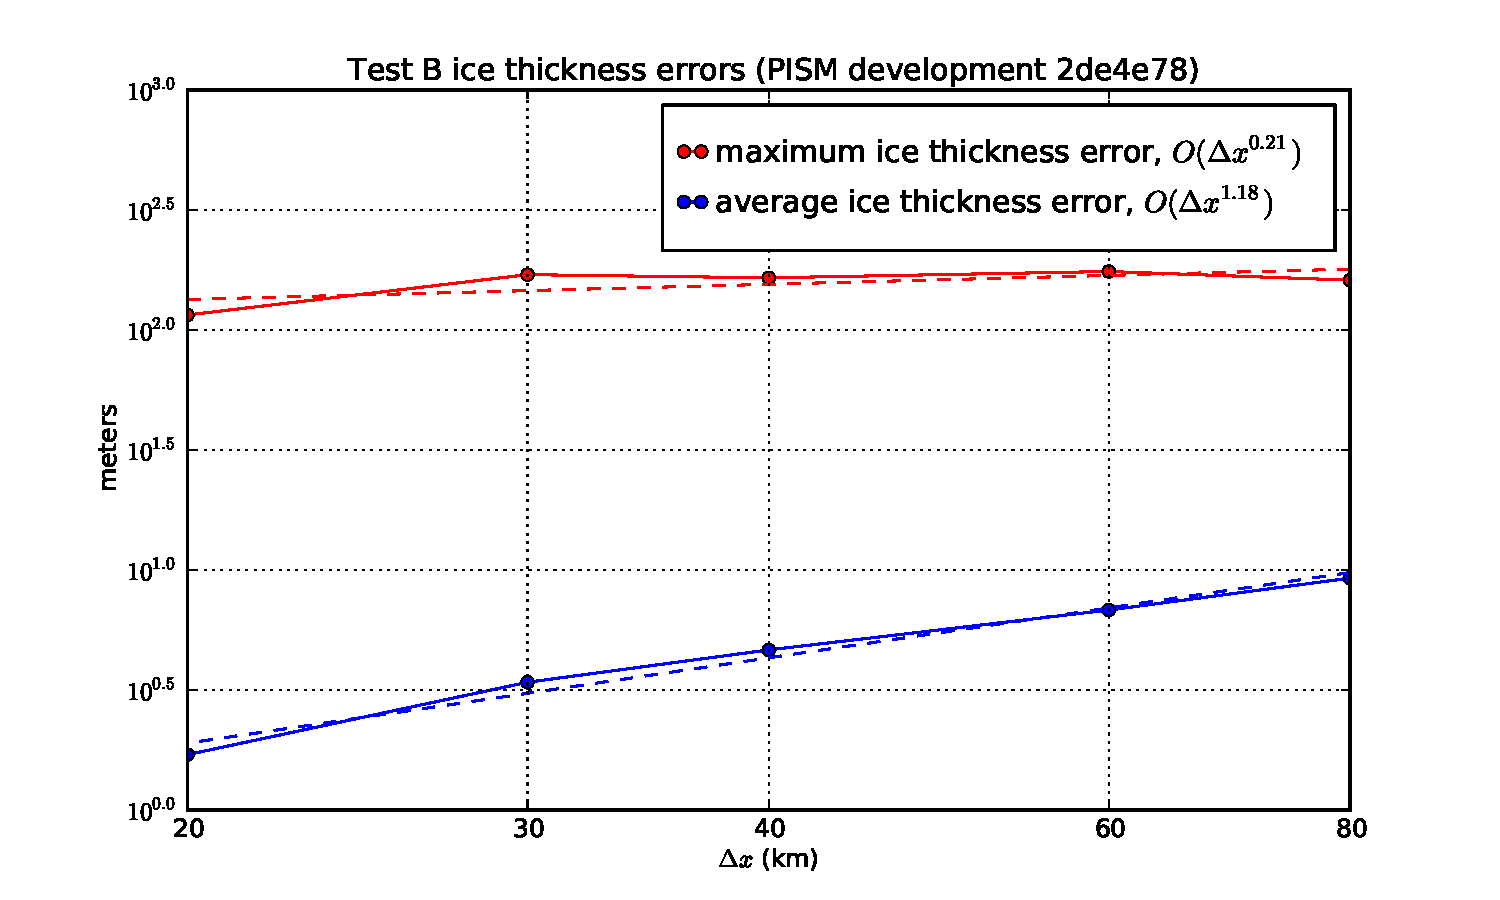
\includegraphics[width=5.0in,keepaspectratio=true]{test-B-thickness}
\caption{Numerical thickness errors in test B. See \cite{BLKCB} for discussion.}
\label{fig:thickerrsB}
\end{figure}

\begin{figure}[ht]
\centering
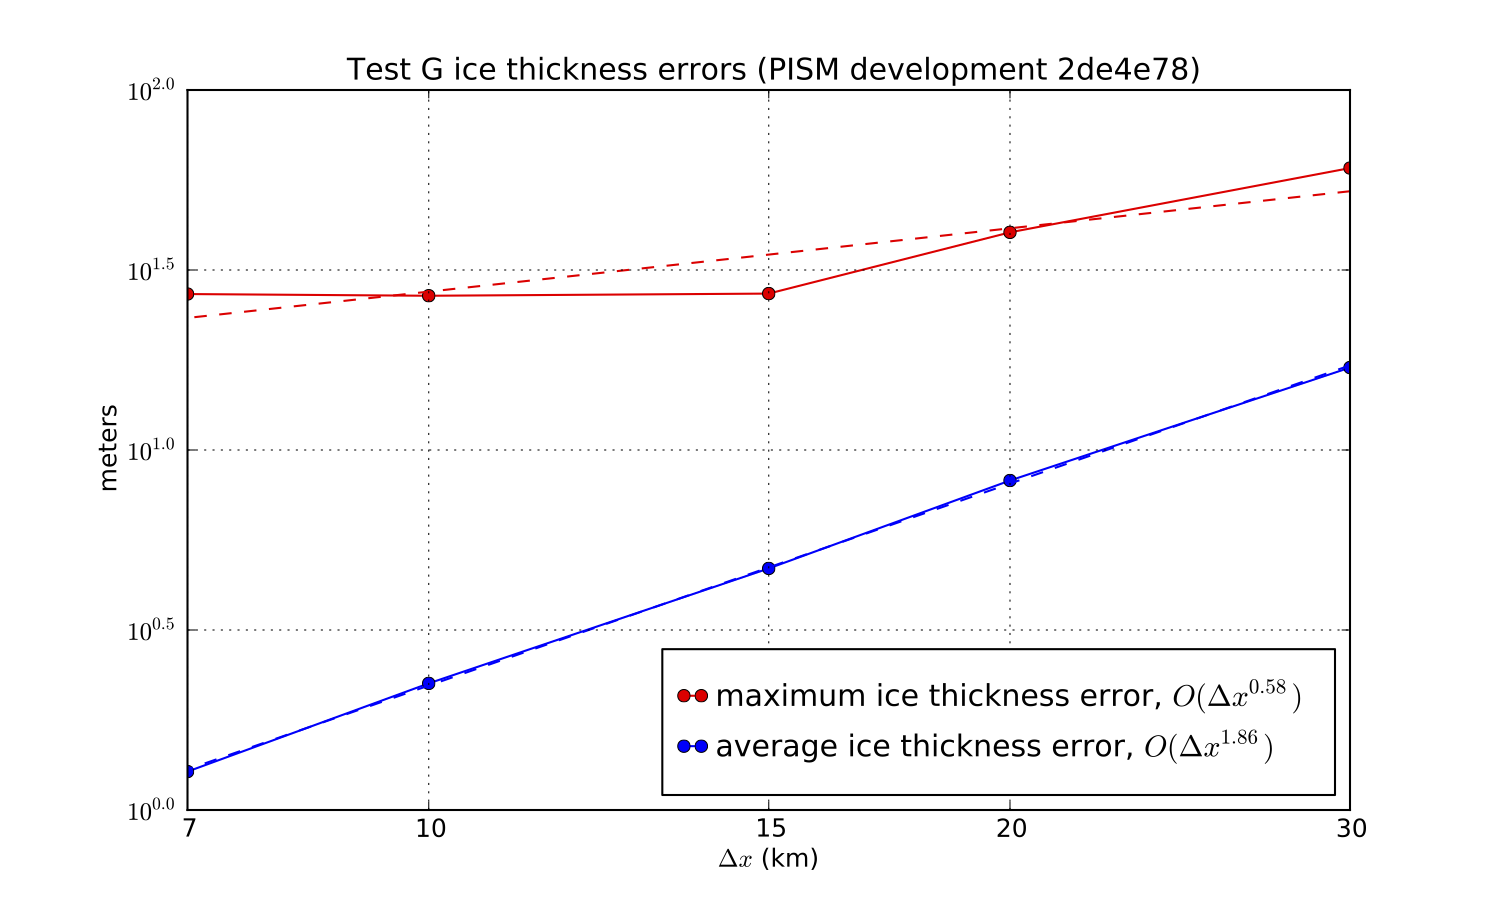
\includegraphics[width=5.0in,keepaspectratio=true]{test-G-thickness}
\caption{Numerical thickness errors in test G.  See \cite{BBL} and \cite{BLKCB}.}
\label{fig:thickerrsG}
\end{figure}

\begin{figure}[ht]
\centering
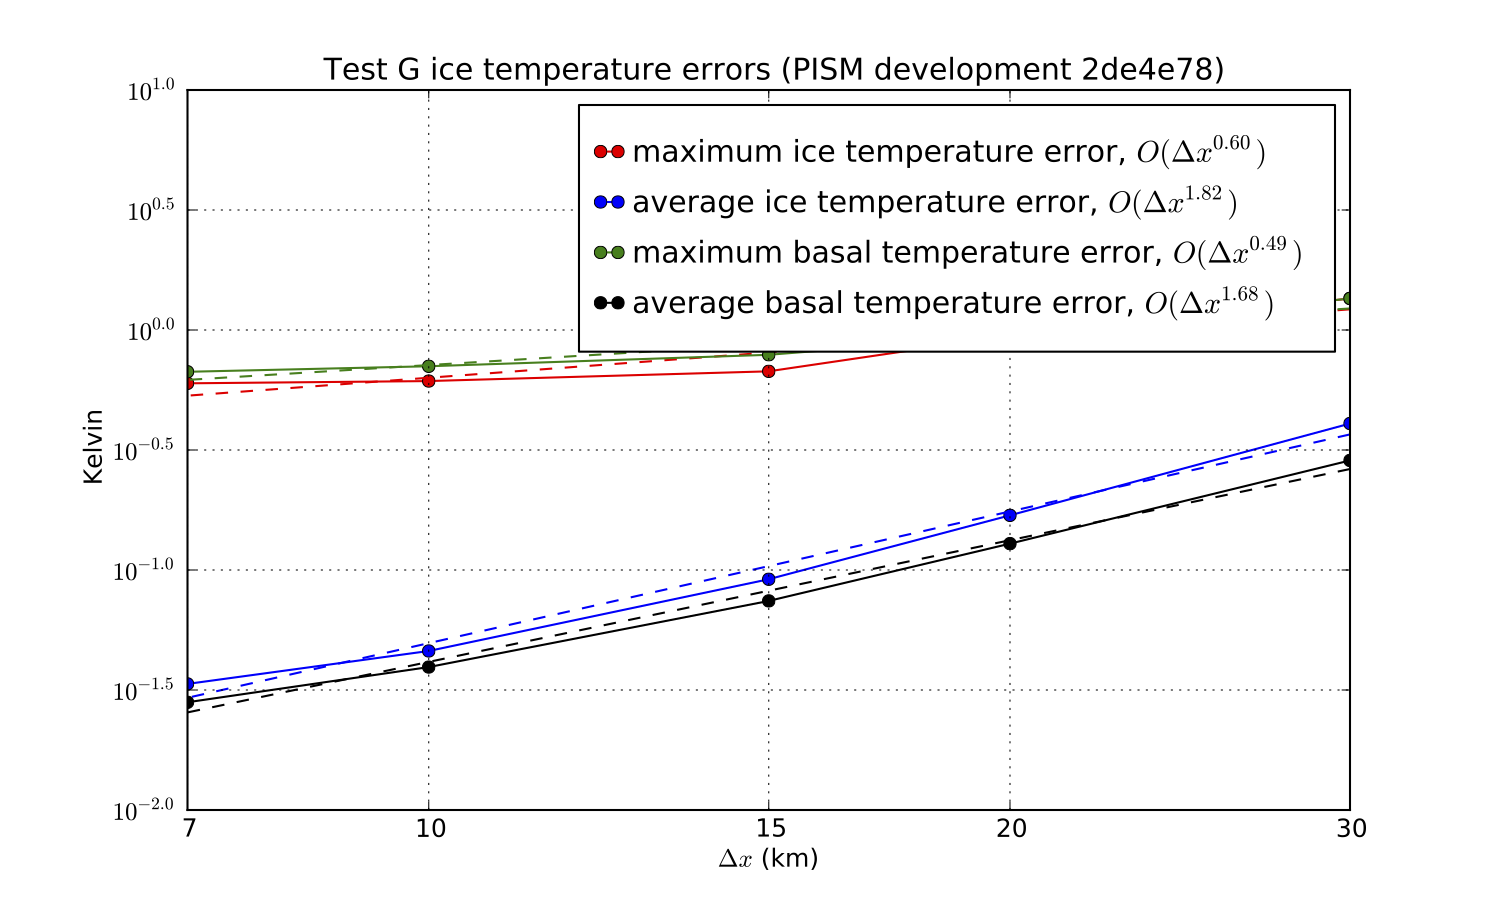
\includegraphics[width=5.0in,keepaspectratio=true]{test-G-temp}
\caption{Numerical temperature errors in test G. See \cite{BBL}.}
\label{fig:temperrsG}
\end{figure}

\begin{figure}[ht]
\centering
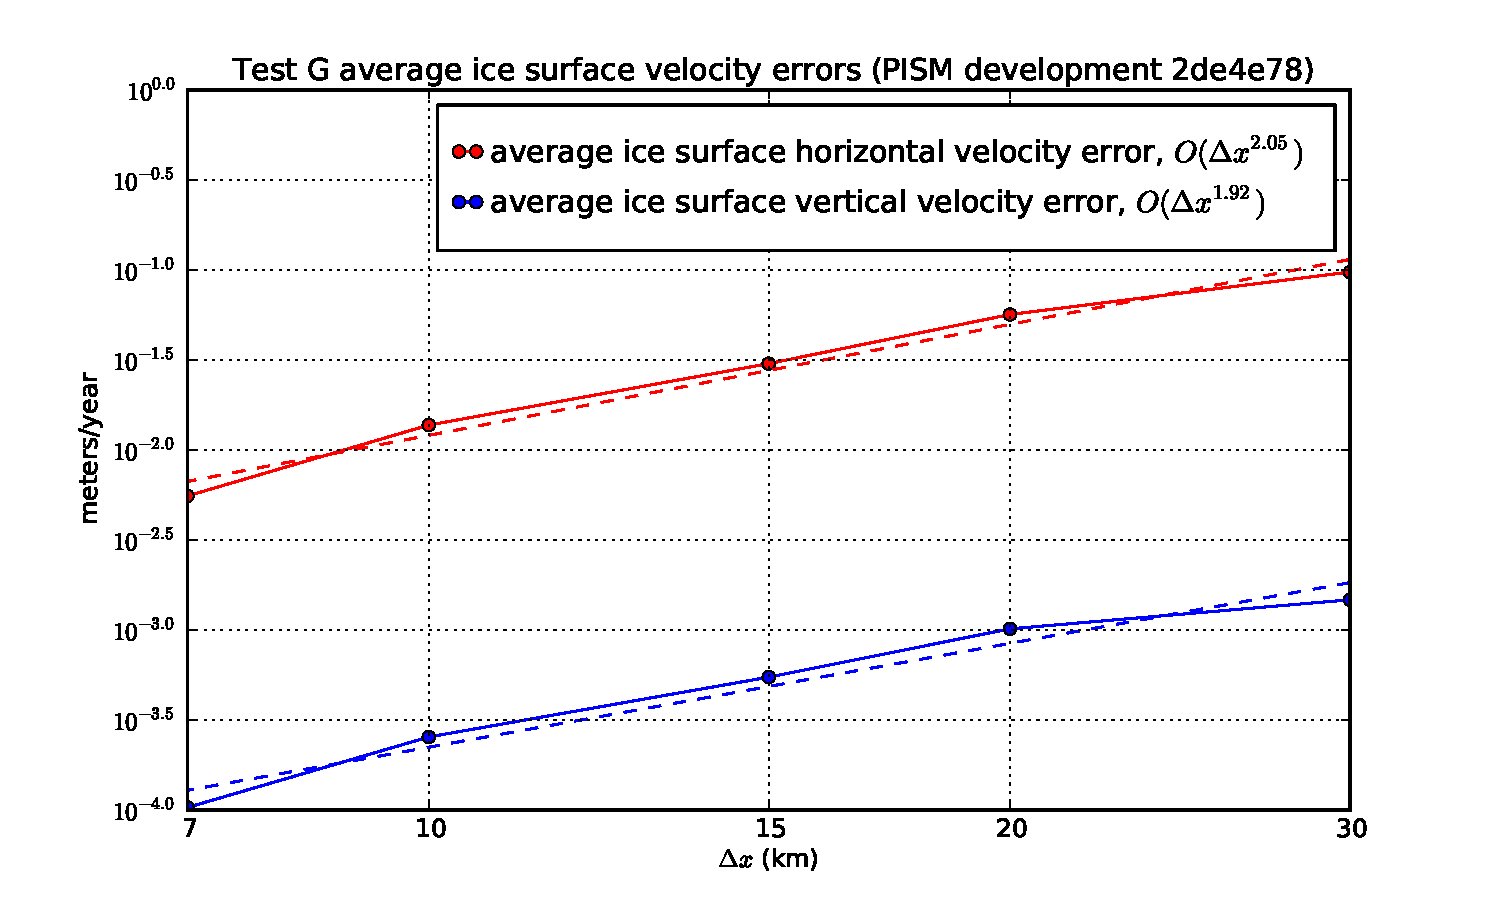
\includegraphics[width=5.0in,keepaspectratio=true]{test-G-surfvels}
\caption{Numerical errors in computed surface velocities in test G.}
\label{fig:surfvelerrsG}
\end{figure}

\begin{figure}[ht]
\centering
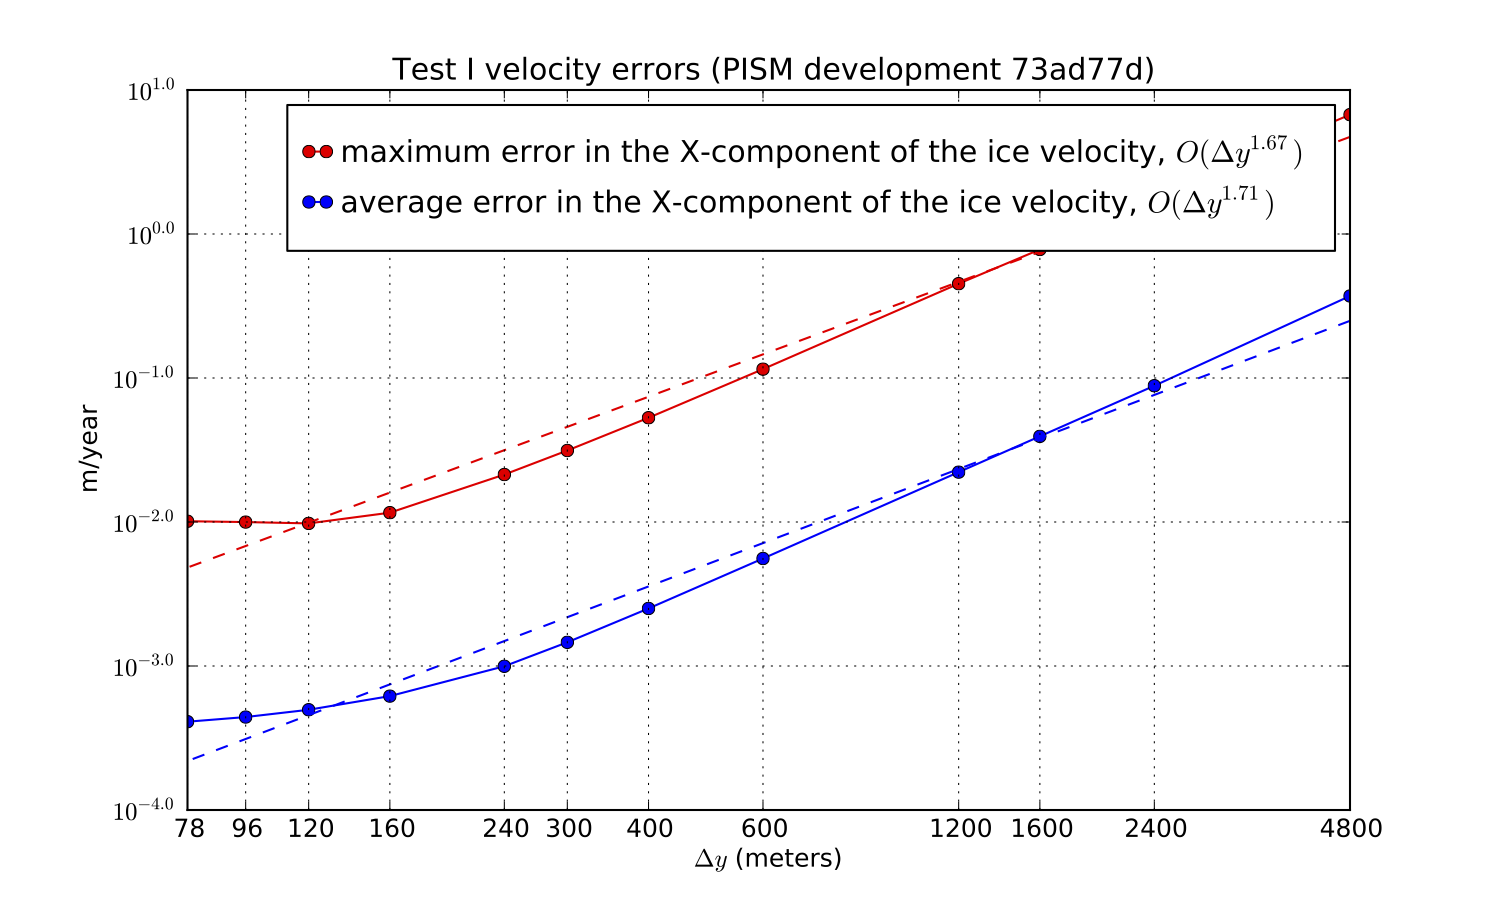
\includegraphics[width=5.0in,keepaspectratio=true]{test-I-errors}
\caption{Numerical errors in horizontal velocities in test I, an ice stream. See \cite{SchoofStream,BBssasliding}.}
\label{fig:velerrsI}
\end{figure}

%%% Local Variables: 
%%% mode: latex
%%% TeX-master: "manual"
%%% End: 


\clearpage\newpage

\section{Simplified geometry experiments with PISM}\label{sec:simp}

There have been three stages of ice sheet model intercomparisons based on simplified geometry experiments since the early 1990s \cite{BuelerSpray}.\index{EISMINT!defined}

EISMINT I \cite[ European Ice Sheet Modeling INiTiative]{EISMINT96}\footnote{See \url{http://homepages.vub.ac.be/\%7Ephuybrec/eismint.html}.} was the first of these and involved only the isothermal shallow ice approximation (SIA).  Both fixed margin and moving margin experiments were performed in EISMINT I, and various conclusions were drawn about the several numerical schemes used in the intercomparison.  EISMINT I is superceded, however, by verification using the full variety of known exact solutions to the isothermal SIA \cite{BLKCB}.  The ``rediscovery'', since EISMINT I, of the Halfar similarity solution with zero accumulation \cite{Halfar83}, and verification runs using that solution, already suffices to measure the isothermal SIA performance of PISM more precisely than would be allowed by comparison to EISMINT I results.

EISMINT II \cite{EISMINT00} pointed out interesting and surprising properties of the thermocoupled SIA.  References \cite{BBL,Hindmarsh04,Hindmarsh06,PayneBaldwin,SaitoEISMINT,BBssasliding} each interpret the EISMINT II experiments and/or describe attempts to add more complete physical models to ``fix'' the (perceived and real) shortfalls of ice sheet model behavior on EISMINT II experiments.  We believe that the discussion in \cite{PayneDongelmans,PayneBaldwin,BBL} adequately explains the ``spokes'' in EISMINT II experiment F as a genuine fluid instability, while \cite{Fowler01} and Appendix B of \cite{BBssasliding} adequately cautions against the continuum model that generates the ``spokes'' in EISMINT II experiment H.   Thus we can move on from that era of controversy.  In any case, PISM has built-in support for all of the published and unpublished EISMINT II experiments; these are described in the next subsection.

The ISMIP (Ice Sheet Model Intercomparison Project)\footnote{See \url{http://homepages.vub.ac.be/\%7Ephuybrec/ismip.html}.}\index{ISMIP!defined} round of intercomparisons covers 2008--2013 (at least).  There are four components of ISMIP substantially completed, namely HOM = Higher Order Models \cite{ISMIPHOM,HOMelmer}, HEINO = Heinrich Event INtercOmparison \cite{GreveTakahamaCalov,Calovetal2009HEINOfinal}, MISMIP (below), and MISMIP3d (also below).

PISM participated in HEINO, but this ability is unmaintained.   We believe\index{ISMIP!interpretation of HEINO results} the continuum problem described by HEINO, also used in EISMINT II experiment H (above), is not meaningfully approximate-able because of a required discontinuous jump in the basal velocity field.  The continuum problem predicts infinite vertical velocity because of this jump \cite[Appendix B]{BBssasliding}.  Details of the numerical schemes and their results are irrelevant if the continuum model makes such a prediction.  PISM offers the physical continuum model described in \cite{BBssasliding}, an SIA+SSA hybrid, as an alternative to the continuum model used in ISMIP-HEINO and EISMINT II experiment H.  Indeed the SIA+SSA hybrid is offered as a unified shallow model for real ice sheets (section \ref{sec:dynamics}).

There is no current plan to support ISMIP-HOM \cite{ISMIPHOM,HOMelmer}, but comparison of shallow PISM results to exact Stokes solutions is a goal for PISM evaluation.

A third and fourth ISMIP parts are the two parts of the Marine Ice Sheet Model Intercomparison Project, MISMIP\index{ISMIP!MISMIP} \cite{MISMIP2012} and MISMIP3D\index{ISMIP!MISMIP3d} \cite{MISMIP3d2013}.  These experiments are supported in PISM, as described in subsections \ref{subsect:MISMIP} and \ref{subsect:MISMIP3d} below.


\subsection{EISMINT II}\label{subsect:EISMINTII}
\optsection{EISMINT II}

There are seven experiments described in the published EISMINT II writeup \cite{EISMINT00}.\index{EISMINT}  They are named A, B, C, D, F, G, and H.  They have these common features:\begin{itemize}
\item runs are for 200,000 years, with no prescribed time step;
\item a $61\times 61$ horizontal grid on a square domain ($1500$ km side length) is prescribed;
\item surface inputs (temperature and mass balance) have angular symmetry around the grid center;
\item the bed is flat and does not move (no isostasy);
\item the temperature in the bedrock is not modeled;
\item only the cold (not polythermal) thermomechanically-coupled SIA is used \cite{EISMINT00}; and
\item basal melt rates do not affect the evolution of the ice sheet.
\end{itemize}
The experiments differ from each other in their various combinations of surface temperature and mass balance parameterizations.  Experiments H and G involve basal sliding, under the physically-dubious SIA sliding rubric \cite[Appendix B]{BBssasliding}, while the others don't.  Four experiments start with zero ice (A,F,G,H), while the other experiments (B,C,D) start from the final state of experiment A.

In addition to the seven experiments published in \cite{EISMINT00}, there were an additional five experiments described in the EISMINT II intercomparison description 
\cite{EISIIdescribe}, labeled E, I, J, K, and L.\index{EISMINT!unpublished additional EISMINT II experiments}  These experiments share most features listed above, but with the following differences.  Experiment E is the same as experiment A except that the peak of the accumulation, and also the low point of the surface temperature, are shifted by 100 km in both $x$ and $y$ directions; also experiment E starts with the final state of experiment A.  Experiments I and J are similar to experiment A but with non-flat ``trough'' bed topography.  Experiments K and L are similar to experiment C but with non-flat ``mound'' bed topography.

See table \ref{tab:eisII} for how to run all EISMINT II experiments in PISM.  Note that the vertical grid is not specified in EISMINT II, but it seems that good simulation of the thermomechanically-coupled conditions near the base of the ice requires relatively-fine resolution there.  (It is difficult to be quantitative because of a lack of theory.)  We suggest using the default unequally-spaced grid with 61 levels, which gives a grid spacing of 18 m in the ice layer closest to the bed.  Alternatively these experiments can be done with an equally-spaced grid; in this case we suggest using 201 vertical levels to give 20 m spacing, for example.

These SIA-only simulations parallelize well.  Very roughly, for the standard $61\times 61$ horizontal grid, wall-clock-time speedups will occur up to about 30 processors.  Runs on finer (horizontal) grids will benefit from even more processors.

Table \ref{tab:eisII} shows how all EISMINT II experiments are done in PISM.  Experiments below the horizontal line in Table \ref{tab:eisII} are only documented in \cite{EISIIdescribe}.

\begin{table}[ht]
\centering
\small
\begin{tabular}{@{}llll}\toprule
\textbf{Command: ``\texttt{pisms }'' $+$} & \textbf{Relation to experiment A} \\
\midrule
\texttt{-eisII A -Mx 61 -My 61 -Mz 61 -y 200000 -o eisIIA.nc} & \\
\texttt{-eisII B -i eisIIA.nc -y 2e5 -o eisIIB.nc} & warmer \\
\texttt{-eisII C -i eisIIA.nc -y 2e5 -o eisIIC.nc} & less snow (lower accumulation)\\
\texttt{-eisII D -i eisIIA.nc -y 2e5 -o eisIID.nc} & smaller area of accumulation \\
\texttt{-eisII F -Mx 61 -My 61 -Mz 61 -y 2e5 -o eisIIF.nc} & colder; famous spokes \cite{BBL} \\
\texttt{-eisII G -Mx 61 -My 61 -Mz 201 -y 2e5 -o eisIIG.nc} & sliding (regardless of temperature) \\
\texttt{-eisII H -Mx 61 -My 61 -Mz 201 -y 2e5 -o eisIIH.nc} & melt-temperature activated sliding \\ \midrule
\texttt{-eisII E -i eisIIA.nc -y 2e5 -o eisIIE.nc} & shifted climate maps \\
\texttt{-eisII I -Mx 61 -My 61 -Mz 201 -y 2e5 -o eisIII.nc} & trough topography \\
\texttt{-eisII J -i eisIII.nc -y 2e5 -o eisIIJ.nc} & trough topography and less snow \\
\texttt{-eisII K -Mx 61 -My 61 -Mz 201 -y 2e5 -o eisIIK.nc} & mound topography \\
\texttt{-eisII L -i eisIIK.nc -y 2e5 -o eisIIL.nc} & mound topography and less snow \\
\bottomrule
\normalsize
\end{tabular}
\caption{Running the EISMINT II experiments in PISM.\index{PISM!running the EISMINT II experiments in}  Use \texttt{-skip -skip_max 5}, on the $61\times 61$ default grid, for significant speedup.}
\label{tab:eisII}
\end{table}

The EISMINT II experiments can be run with various modifications of the default settings.  Of course the grid can be refined.  For instance, a twice as fine grid in the horizontal is ``\texttt{-Mx 121 -My 121}''.  Table \ref{tab:eisIIoptions} lists some optional settings which are particular to the EISMINT II experiments.

\begin{table}[ht]
\centering
\small
\begin{tabular}{@{}lllp{0.45\linewidth}}\toprule
\textbf{Option} & \textbf{Default values [expers]} & \textbf{Units} & \textbf{Meaning} \\\midrule
\intextoption{eisII} & A & &  Choose single character name of EISMINT II \cite{EISMINT00} simplified geometry experiment.  See Table \ref{tab:eisII}. \\
\intextoption{Mmax} & 0.5 [ABDEFGHIK], 0.25 [CJL] & m$/$a & max value of accumulation rate \\
\intextoption{Rel} & 450 [ABEFGHIK], 425 [CDJL] & km & radial distance to equilibrium line \\
\intextoption{Sb} & $10^{-2}$ [\emph{all}] & (m/a)/km & radial gradient of accumulation rate \\
\intextoption{ST} & $1.67 \times 10^{-2}$ [\emph{all}] & K/km & radial gradient of surface temperature\\
\intextoption{Tmin} & 238.15 [ACDEGHIJKL], & K & max of surface temperature \\
 & 243.15[B], 223.15[F] & & \\
\intextoption{bmr_in_cont} & & & Include the basal melt rate in the mass continuity computation; overrides EISMINT II default. \\
\bottomrule\normalsize
\end{tabular}
\caption{Changing the default settings for EISMINT II}
\label{tab:eisIIoptions}
\end{table}

In PISM the height of the computational box, the quantity set by \texttt{-Lz}, is set at the beginning of the run.  It is chosen for the EISMINT II experiments according to the observed maximum values occuring in standard runs.  If the ice thickens beyond the chosen level for the top of the computational box then additional layers are automatically added to the computational grid.  In fact, if the ice grows above the height of the computational box then a message appears, \texttt{PISM WARNING: max ice thickness ... is greater than the height of the computational box ...}, and then at least two additional levels are added to the vertical grid.  However, in general this mechanism can run away to use up all memory in extreme cases so, if the height of the computational box grows so large that the grid has more than twice the original number of vertical levels, then PISM produces an error message and stops.   Therefore it is possible that the number of vertical levels at the end of the run exceeds the initial \texttt{-Mz} value.  Setting EISMINT II options \texttt{-Mmax} or \texttt{-Sb} to produce higher accumulation rates than the default values (see table \ref{tab:eisIIoptions}) may cause the ice sheet to thicken above the standard thickness and therefore trigger this automatic extension mechanism.  Similarly, colder ice caused by nonstandard \texttt{-Tmin} or \texttt{-ST} values can produce unusually thick ice.  The user may always choose to use a larger, more conservative value for option \texttt{-Lz}, however.

See subdirectory \verb|examples/eismintII/| for a simple helper script \verb|runexp.sh|.


\subsection{MISMIP}\label{subsect:MISMIP}
\optsection{MISMIP}\index{ISMIP!MISMIP}

This intercomparison addresses grounding line dynamics by considering an idealized one-dimensional stream-shelf system.  In summary, a flowline ice stream and ice shelf system is modeled, the reversibility of grounding line movement under changes in the ice softness is tested, different sliding laws are tested, and the behavior of grounding lines on reverse-slope beds is tested.  The intercomparison process is described at the website

\centerline{\url{http://homepages.ulb.ac.be/~fpattyn/mismip/}}

\noindent Find a full text description there, along with the published report on the results \cite{MISMIP2012}; that paper includes results from PISM version 0.1.  These documents are essential reading for understanding MISMIP results generally, and for appreciating the brief discussion in this subsection.

PISM's version of MISMIP includes an attached ice shelf even though modeling the shelf is theoretically unnecessary in the flow line case.  The analysis in \cite{SchoofMarine1} shows that the only effect of an ice shelf, in the flow line case, is to transfer the force imbalance at the calving front directly to the ice column at the grounding line.  Such an analysis does not apply to ice shelves with two horizontal dimensions; real ice shelves have ``buttressing'' and ``side drag'' and other forces not present in the flow line \cite{Goldbergetal2009}.  See the next subsection on MISMIP3d and the Ross ice shelf example in section \ref{sec:ross}, among other examples.

We must adapt the usual 3d PISM model to two horizontal dimensions, i.e.~to do flow-line problems (see section \ref{sec:flowline-modeling}).  The flow direction for MISMIP is taken to be ``$x$''.  We periodize the cross-flow direction ``$y$'', and use the minimum number of points in the $y$-direction.  This number turns out to be ``\texttt{-My 3}''; fewer points than this in the cross-flow direction confuses the finite difference scheme.

PISM can do MISMIP experiments with either of two applicable ice dynamics models.  Model 1 is a pure SSA model; ``category 2'' in the MISMIP classification.  Model 2 combines SIA and SSA velocities as described in \cite{Winkelmannetal2011}; ``category 3'' because it resolves ``vertical'' shear (i.e.~using SIA flow).

There are many runs for a complete MISMIP intercomparison submission.  Specifically, for a given model there are $62$ runs for each grid choice, and three (suggested) grid choices, so a full suite is $3 \times 62 = 186$ runs.

The coarsest grid (``mode 1'') has 12 km spacing.  The finest grid, ``mode 2'' with 1.2 km spacing, accounts for all the compute time, however; in the MISMIP description it is 1500 grid spaces in the flow line direction (= 3001 grid \emph{points} in PISM's doubled computational domain).  In between is ``mode 3'', a mode interpretable by the intercomparison participant, and here we just use a 6 km grid.

The implementation of MISMIP in PISM conforms to the intercomparison description, but that document specifies
\begin{quotation}
\dots we require that the rate of change of grounding line position be $0.1$ m/a or less, while the rate of change of ice thickness at each grid point at which ice thickness is defined must be less than $10^{-4}$ m/a \dots
\end{quotation}
as a standard for ``steady state''.  The scripts here do not implement this stopping criterion.  However, we report enough information, in PISM output files with scalar and spatially-variable time-series, to compute a grounding line rate or the time at which the thickness rate of change drops below $10^{-4}$ m/a.

See

  \centerline{\texttt{examples/mismip/mismip2d/README.md}}

\noindent for usage of the scripts that run MISMIP experiments in PISM.  For example, as described in this \texttt{README.md}, the commands

\begin{verbatim}
$ ./run.py -e 1a --mode=1 > experiment-1a-mode-1.sh
$ bash experiment-1a-mode-1.sh 2 >& out.1a-mode-1 &
$ ./plot.py ABC1_1a_M1_A7.nc -p -o profileA7.png
\end{verbatim}

\noindent first generate a bash script, then use it to do a run which takes about 20 minutes, and then generate an image in \texttt{.png} format.  Note that step 7 is in the middle of the experiment.  It is shown in Figure \ref{fig:MISMIPmodel1exper1aA7} (left).
 
\begin{figure}[ht]
\centering
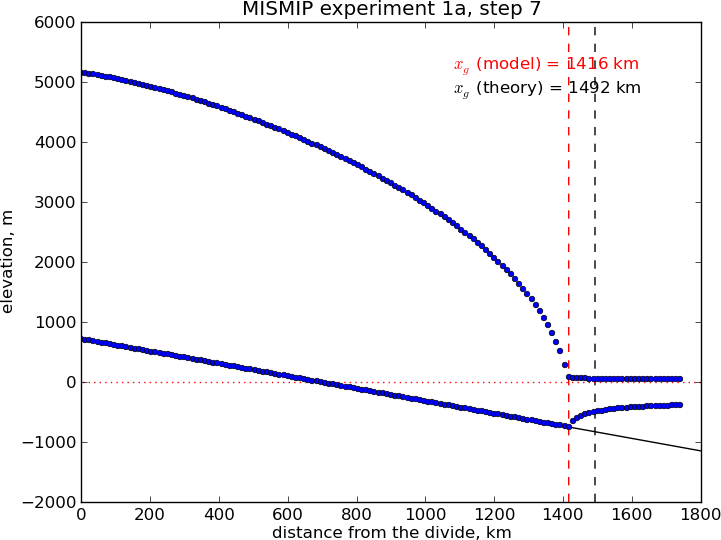
\includegraphics[width=3.3in,keepaspectratio=true]{profileA7} \,
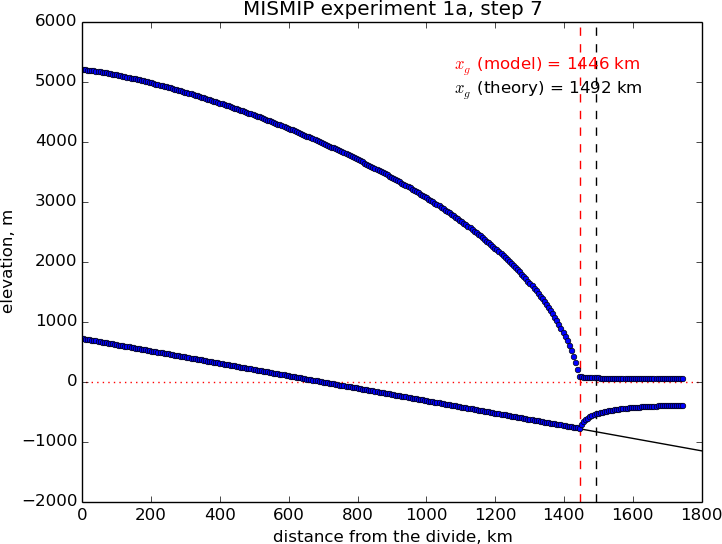
\includegraphics[width=3.3in,keepaspectratio=true]{profileA7-M3}
\caption{A marine ice sheet profile in the MISMIP intercomparison; PISM model 1, experiment 1a, at step 7.  Left: grid mode 1 (12 km grid).  Right: grid mode 3 (6 km grid).}
\label{fig:MISMIPmodel1exper1aA7}
\end{figure}

\begin{figure}[ht]
\centering
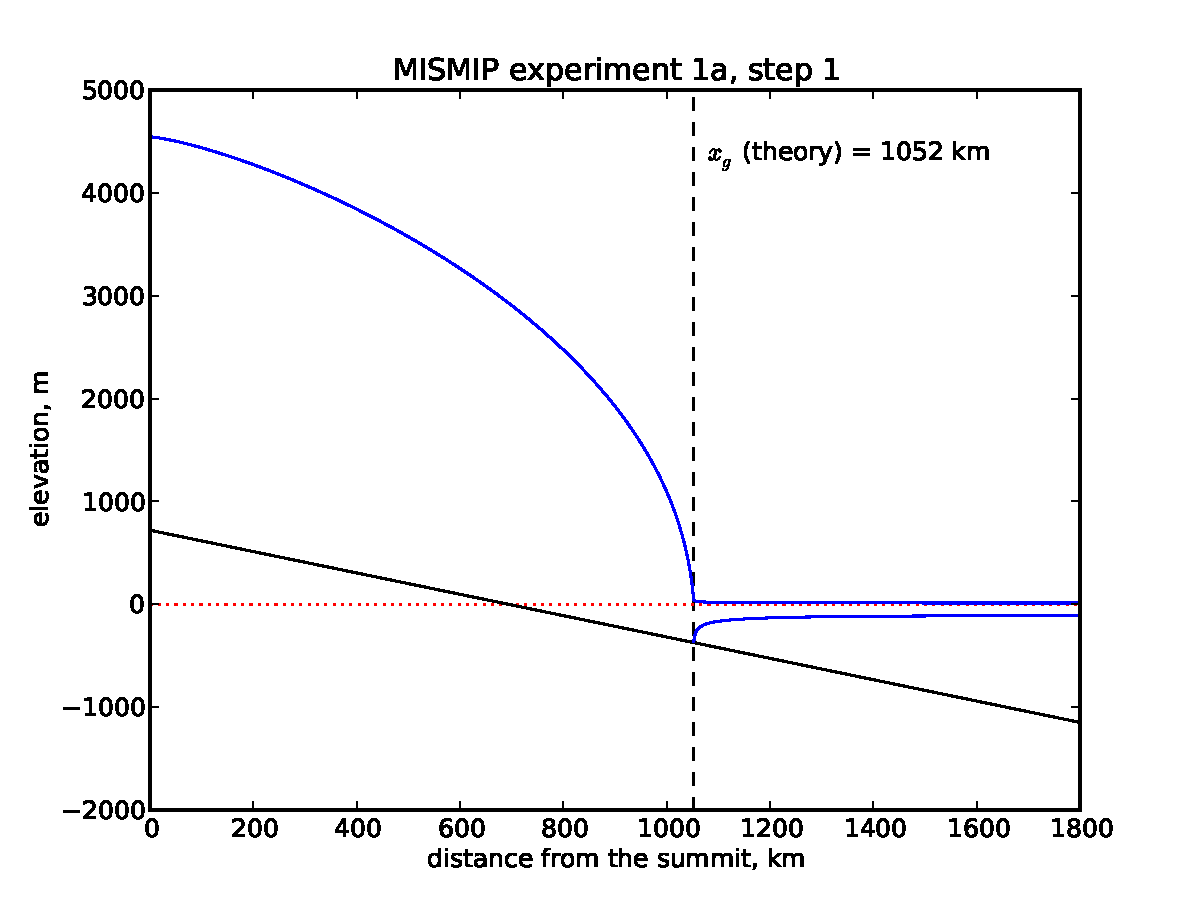
\includegraphics[width=4.0in,keepaspectratio=true]{SM-1a-A1}
\caption{Analytical profile for steady state of experiment 1a, step 1, from theory in \cite{SchoofMarine1}.  This is a boundary layer asymptotic matching result, but not the exact solution to the equations.}
\label{fig:SMexper1aM1A1}
\end{figure}

The script \texttt{MISMIP.py} in \texttt{examples/mismip/mismip2d} has the ability to compute the profile from the Schoof's \cite{SchoofMarine1} asymptotic-matching boundary layer theory.  This script is a Python translation, using \texttt{scipy} and \texttt{pylab}, of the \Matlab codes in \url{http://homepages.ulb.ac.be/~fpattyn/mismip/MISMIP_distribution.tar}.  For example,

\begin{verbatim}
$ python MISMIP.py -o mismip_analytic.png
\end{verbatim}
 
\noindent produces a \verb|.png| image file with Figure \ref{fig:SMexper1aM1A1}.  By default \texttt{run.py} uses the asymptotic-matching thickness result from the \cite{SchoofMarine1} theory to initialize the initial ice thickness, as allowed by the MISMIP specification.

\begin{figure}[ht]
\centering
\includegraphics[width=3.3in,keepaspectratio=true]{profileA7-M2}
\caption{Results from MISMIP grid mode 2, with 1.2 km spacing, for steady state of experiment 1a: profile at step 7 (compare Figure \ref{fig:MISMIPmodel1exper1aA7}).}
\label{fig:MISMIPmode2results}
\end{figure}

Generally the PISM result does not put the grounding line in the same location as Schoof's boundary layer theory, and at least at coarser resolutions the problem is with PISM's numerical solution, not with Schoof's semi-analytic theory.  The result improves under grid refinement, however.  Results from grid mode 3 with 6 km spacing, instead of 12 km in mode 1, are the right part of Figure \ref{fig:MISMIPmodel1exper1aA7}.  The corresponding results from grid mode 2, with 1.2 km spacing, are in Figure \ref{fig:MISMIPmode2results}.  Note that the difference between the numerical grounding line location and the semi-analytical location has been reduced from 76 km for grid mode 1 to 16 km for grid mode 2 (a factor of about 5), by using a grid refinement from 12 km to 1.2 km (a factor of about 10).


\subsection{MISMIP3d}\label{subsect:MISMIP3d}
\optsection{MISMIP3d}\index{ISMIP!MISMIP3d}
The ice2sea MISMIP3d intercomparison is a two-horizontal-dimensional extension of the flowline case described above.  As before, in MISMIP3d the grounding line position and its reversibility under changes of physical parameters is analyzed.  Instead of changing the ice softness, however, the spatial distribution and magnitude of basal friction is adjusted between experiments.  The applied basal friction perturbation of the basal friction is a localized gaussian ``bump'' and thus a curved grounding line is obtained.  In contrast to the flowline experiments, no (semi-)analytical solutions are available to compare to the numerical results.

A full description of the MISMIP3d experiments can be found at

\centerline{\url{http://homepages.ulb.ac.be/~fpattyn/mismip3d/}}

\noindent and the results are published in \cite{MISMIP3d2013}.

A complete set of MISMIP3d experiments consists of three runs: Firstly, a flowline solution on a linearly-sloped bed, similar to the flowline MISMIP experiments of the previous section, is run into a steady state (``standard experiment \texttt{Stnd}'').  Then the localized sliding perturbation is applied (``perturbation experiment'')  causing the grounding line to shift and lose symmetry.  Two different amplitudes of the perturbation are considered (``\texttt{P10}'' and ``\texttt{P75}'').  Finally, beginning from the final state of the perturbation experiment, the sliding perturbation is removed and the system is run again into steady state (``reversibility experiment'').  The resulting geometry, in particular the grounding line position, is expected to be close to that of the standard experiment.  Expecting such reversibility assumes that a particular stationary ice geometry only depends on its physical parameters and boundary conditions and not on how it is dynamically reached.

For these experiments in PISM, a Python script generates a shell script which has the commands and options for running a MISMIP3d experiment.  The python script is \texttt{createscript.py} in the folder \texttt{examples/mismip/mismip3d/}.  Run

\begin{verbatim}
$ ./createscript.py -h
\end{verbatim}

\noindent to see a usage message.  A \texttt{README.md} gives a tutorial on how to use \texttt{createscript.py} and do the runs themselves.

For the flowline \texttt{Stnd} experiment, as in the MISMIP case, a computational domain with three grid points in the direction orthogonal to the ice flow (arbitrarily chosen as y-direction) is chosen by \texttt{createscript.py}.  For the perturbation and reversibility experiments a domain is defined which is symmetric along the ice-divide (mirror symmetry) and along the center line of the ice flow, while the side boundaries are periodic, which corresponds to a free-slip condition for the flow in x-direction. Though this choice of the symmetric computational domain increases computational cost, it allows us to use standard PISM without fixing certain boundary conditions in the code.  (That is, it avoids the issues addressed in the regional mode of PISM; see section \ref{sec:jako}.)

PISM participated in the MISMIP3d intercomparison project \cite{MISMIP3d2013} using version \texttt{stable0.5}, and the exact results can be reproduced using that version.  PISM's results, and the role of resolution and the new subgrid grounding line interpolation scheme are discussed in \cite{Feldmannetal2014}.

We observed a considerable improvement of the results with respect to the absolute grounding line positions compared to other models (e.g. the FE reference model Elmer/Ice) and to the reversibility when applying the subgrid grounding line interpolation method; see Figure \ref{fig:Subgl}.  Furthermore, we observed that only using SSA yields almost the same results as the full hybrid SIA+SSA computation for the MISMIP3D (and also the MISMIP) experiments, but, when not applying the SIA computation, after a considerably shorter computation time (about 10 times shorter).  We explain the small and almost negligible SIA velocities for the MISMIP(3D) experiments with the comparably small ice surface gradients in the MISMIP3d ice geometries.  See Fig.~\ref{fig:compSIASSA} for a comparison of SSA and SIA velocities in the MISMIP3D geometry.  Note that both Figures \ref{fig:Subgl} and \ref{fig:compSIASSA} were generated with resolution of $\Delta x = \Delta y = 1\;$km.

\begin{figure}[ht]
\centering
\includegraphics[width=3.3in,keepaspectratio=true]{Subgl}
\includegraphics[width=3.3in,keepaspectratio=true]{NoSubgl}
\caption{Comparison between the grounding lines of the higher-amplitude (``\texttt{P75}'') MISMIP3d experiments performed with PISM when using the subgrid grounding line interpolation method (left) or not using it (right).  In both cases the SIA+SSA hybrid is used.}
\label{fig:Subgl}
\end{figure}

\begin{figure}[ht]
\centering
\includegraphics[width=5.0in,keepaspectratio=true]{comp-SIA-SSA}
\caption{The SIA velocities are negligible in the MISMIP3d standard experiment (``\texttt{Stnd}'').  The steady state ice geometry is plotted (black) together with the computed SSA velocity (red) and SIA velocity (blue). The SIA velocity reaches its maximum value of about $10\,$m/a at the grounding line, about two orders of magnitude less than the maximum of the SSA velocity.}
\label{fig:compSIASSA}
\end{figure}

%%% Local Variables: 
%%% mode: latex
%%% TeX-master: "manual"
%%% End: 


\clearpage\newpage

\section{Example: Modeling the Greenland ice sheet (EISMINT-Greenland)}\label{sec:eismint-greenland} \index{PISM!running the EISMINT-Greenland intercomparison}\index{Ice Sheets!Greenland ice sheet}\index{EISMINT!intercomparison of Greenland models} 
\optsection{EISMINT-Greenland}

In this section we give an extended example of how to use PISM to model the Greenland ice sheet.  We use older data from the 1990s ice sheet modelling intercomparison EISMINT-Greenland \cite{HuybrechtsEISMINT,RitzEISMINT}, but it is an excellent tutorial example.

The data are freely available at

\begin{center}
  \url{http://homepages.vub.ac.be/~phuybrec/eismint/greenland.html}
\end{center}

\noindent The snow-fall accumulation map, ablation parameterization, surface temperature formula, surface elevation, and bedrock elevation maps are essentially as in the 1991 papers \cite{Letreguillyetal1991,OhmuraReeh}.  In the ``forced climate'' CCL3 run, described below, the modeled ice sheet sees changes in surface temperature from the GRIP core \cite{Dansgaardetal1993} and sea level changes from SPECMAP \cite{Imbrieetal1984}.

Substantial developments have occurred in modeling the Greenland ice sheet since the EISMINT-Greenland intercomparison.  For example, the relation between a Greenland ice sheet flow model, Earth deformation under ice sheet loads, and the reconstruction of global ice loading is analyzed in \cite{TarasovPeltier}.  A parameter-sensitivity study of a EISMINT-Greenland-type ice sheet model is described in \cite{RitzFabreLetreguilly}.  The response of Greenland ice sheet models to climate warming is addressed in \cite{HuybrechtsdeWolde,Huybrechts02, Greve00}, among other references.

The rest of this section is a step-by-step PISM tutorial.  The details can be typed in by hand, or the user can invoke the bash scripts \texttt{preprocess.sh}, \texttt{bootstrap.sh}, \texttt{ssl2.sh}, and \texttt{ccl3.sh} in the directory \texttt{examples/eisgreen}.  These scripts execute the commands in the next four subsections, respectively.

\subsubsection*{Obtaining and pre-processing the EISMINT-Greenland data}  We use two Python scripts to convert the EISMINT-Greenland data.  The data is in the form of several ASCII text files, so we convert them into NetCDF files usable by PISM.  The Python libraries \href{http://numpy.scipy.org/}{\texttt{numpy}} and \href{http://code.google.com/p/netcdf4-python/}{\texttt{netcdf4-python}} must be present for the scripts to work.

First, \texttt{cd examples/eisgreen/} from the PISM directory, and download these text (ASCII) files from the EISMINT-Greenland web site above: 

\begin{verbatim}
grid20-EISMINT,  suaq20-EISMINT,  specmap.017,  sum89-92-ss09-50yr.stp
\end{verbatim}

\noindent (This is done by \texttt{preprocess.sh} using \texttt{wget}.) Once all four files have been downloaded, run

\begin{verbatim}
$ ./eisgreen.py
\end{verbatim}%$

\noindent The NetCDF file \texttt{eis_green20.nc} will be created from the data in \texttt{grid20-EISMINT} and \texttt{suaq20-EISMINT}.  It contains variables for the gridded latitude (\texttt{lat}), longitude (\texttt{lon}), surface altitude (``\texttt{usurf}'' for \textbf{u}pper \textbf{surf}ace elevation), ice thickness (\texttt{thk}), bedrock altitude (\texttt{topg}), and snow precipitation rate (\texttt{precip}; in ice-equivalent thickness units).  These values can be viewed graphically with \texttt{ncview}.  The metadata for these variables (the NetCDF ``header'') can be viewed by

\begin{verbatim}
ncdump -h eis_green20.nc
\end{verbatim}

The bed elevation \texttt{topg} in the original data (\texttt{suaq20-EISMINT}) effectively contains missing values.  These are locations where \texttt{topg} is \emph{exactly} $0.0$, presumably because in these locations the observed bed elevation was not measured or the measured value was not trusted.  We think these are deep fjords locations, mostly.  Also the topography of Ellesmere island is replaced by out of range negative values.  When viewing \texttt{eis_green20.nc} with \texttt{ncview}, these values show as white spots.  

If these missing values were to be left in the NetCDF handed to PISM then the resulting (very) rough bed elevation map would make reasonable ice flow results difficult.  We therefore smoothly fill the holes in the bed elevations.  This is done with another script named \texttt{fill_missing.py}\index{executables!python scripts!\texttt{fill_missing.py}}:\footnote{\texttt{fill_missing.py} is a general tool for smoothly filling patches of missing values in variables in NetCDF files.  It looks for attributes defining missing values and then fills in specified variables essentially by averaging the neighboring non-missing values.  It is found in directory \texttt{pism/util/}, it requires \href{http://code.google.com/p/netcdf4-python/}{\texttt{netcdf4-python}}, and it is documented in subsection \ref{subsect:scripts}.}:

\begin{verbatim}
$ fill_missing.py -f eis_green20.nc -v topg -o eis_green_smoothed.nc
\end{verbatim}%$

\begin{figure}[ht]
\centering
\includegraphics[width=2.4in,keepaspectratio=true]{EISgreen-thick}\quad\includegraphics[width=2.4in,keepaspectratio=true]{EISgreen-bed}
\caption{Views of the thickness (left) and smoothed bed elevation (right) for EISMINT-Greenland.  The coastal topography around several fjords has been smoothed.}
\label{fig:greendata}
\end{figure}

Next we use a script which converts the time-series data files \texttt{specmap.017} and \texttt{sum89-92-ss09-50yr.stp} to PISM-readable NetCDF form:

\begin{verbatim}
$ ./eiscore.py
\end{verbatim}%$

\noindent Two NetCDF files with one-dimensional time series data are created, namely \texttt{grip_dT.nc} and \texttt{specmap_dSL.nc}.  In the paleoclimate run ``CCL3'' below, the executable \texttt{pgrn} will be called with options \texttt{-dTforcing} and \texttt{-dSLforcing} on these two \texttt{.nc} files, respectively.  Thus PISM will read the GRIP data \cite{Dansgaardetal1993} for the surface temperature forcing and the SPECMAP data \cite{Imbrieetal1984} for sea level forcing.  Figure \ref{fig:gripDeltaT} shows the GRIP temperature offsets.

\begin{figure}[ht]
\centering
\includegraphics[width=5.6in,keepaspectratio=true]{gripDeltaT}
\caption{Change in temperature from present, from the GRIP core \cite{JohnsenetalGRIP}.}
\label{fig:gripDeltaT}
\end{figure}


\subsubsection*{Bootstrapping}  \label{sect:green-bootstrapping}  Once the EISMINT Greenland data is obtained and converted to NetCDF, as above, ``bootstrapping'' can begin.  By ``bootstrapping'' we mean the creation, by heuristics and simplified models, of the full initial conditions needed for the continuum model.  \footnote{The continuum model is the differential equations describing ice flow inside PISM.  See section \ref{sect:boot} for more on ``bootstrapping''.}

We do a one model year run using option \texttt{-boot_file} to ``bootstrap'' from file \texttt{eis_green_smoothed.nc}.  The executable ``\texttt{pgrn}'' is special to EISMINT-Greenland\footnote{It sets EISMINT-Greenland parameters and implements the elevation- and latitude-dependent near-surface air temperature parameterization but shares all the ice-dynamics code with \texttt{pismr}.}: \index{executables!\texttt{pgrn}}
% pgrn -boot_file eis_green_smoothed.nc -Mx 83 -My 141 -Lz 4000 -Mz 51 -Lbz 2000 -Mbz 21 -skip 1 -y 1 -o green20km_y1.nc
\begin{verbatim}
$ pgrn -boot_file eis_green_smoothed.nc -Mx 83 -My 141 -Lz 4000 -Mz 51 -Lbz 2000 -Mbz 21\
       -skip 1 -y 1 -o green20km_y1.nc
\end{verbatim}%$
\noindent The run takes only a few seconds of real time on any machine.  Tables \ref{bootstrapEISgreen} and \ref{bootCONTINUED} show the entire PISM output at the terminal.

\begin{table}
\centering
\scriptsize
\begin{quote}
\begin{verbatim}
PGRN trunk 0.4.1732 (PISM EISMINT-Greenland mode)
  setting flags equivalent to '-e 3 -ocean_kill'; user options may override ...
Setting PDD parameters to EISMINT-Greenland values...
  pdd_factor_ice  = 0.00879 m (ice equivalent) K-1 day-1
  pdd_factor_snow = 0.00330 m (ice equivalent) K-1 day-1
  pdd_refreeze    = 0.60000 1
  pdd_std_dev     = 5.00000 K
  time dimension was not found; setting current year to 0.0 years
  setting flow law to polythermal type ...
* Initializing bed smoother object with 5.000 km half-width ...
* Initializing the SIA stress balance modifier...
* Initializing Greenland atmosphere model based on the EISMINT Greenland (C. Ritz, 1997)
  air temperature parameterization and using stored time-independent precipitation...
    reading mean annual ice-equivalent precipitation rate 'precip'
      from eis_green_smoothed.nc ... 
  FOUND  precip    / mean annual ice-equivalent precipitation rate
                   \ min,max =     0.030,    2.820 (m year-1)
* Initializing the default temperature-index, PDD-based surface processes scheme.
  Precipitation and 2m air temperature provided by atmosphere are inputs.
  Surface mass balance and ice upper surface temperature are outputs.
  See PISM User's Manual for control of degree-day factors.
  Computing number of positive degree-days by: an expectation integral.
* Initializing the constant ocean model...
bootstrapping by PISM default method from file eis_green_smoothed.nc
  rescaling computational box for ice from -boot_file file and
    user options to dimensions:
    [-820.00 km, 820.00 km] x [-1400.00 km, 1400.00 km] x [0 m, 4000.00 m]
  WARNING: surface elevation 'usurf' found; IGNORING IT!
  reading 2D model state variables by regridding ...
  FOUND  lon       / standard_name=longitude 
                   \ min,max =   -94.194,   12.889 (degree_east)
  FOUND  lat       / standard_name=latitude  
                   \ min,max =    58.275,   84.458 (degree_north)
  FOUND  thk       / standard_name=land_ice_thickness
                   \ min,max =     0.000, 3200.000 (m)
  FOUND  topg      / standard_name=bedrock_altitude
                   \ min,max = -3859.000, 2151.000 (m)
  absent bwat      / effective thickness of subglacial melt water
                   \ not found; using default constant    0.00 (m)
  absent bmelt     / ice basal melt rate in ice thickness per time
                   \ not found; using default constant    0.00 (m year-1)
  absent bheatflx  / upward geothermal flux at bedrock surface
                   \ not found; using default constant   50.00 (mW m-2)
  absent dbdt      / bedrock uplift rate
                   \ not found; using default constant    0.00 (m year-1)
  filling in ice and bedrock temperatures using surface temps and quartic guess
  ice enthalpy set from temperature, as cold ice (zero liquid fraction)
done reading eis_green_smoothed.nc; bootstrapping done
\end{verbatim}
\end{quote}
\normalsize
\bigskip
\caption{Output of bootstrapping command.  Continues in Table \ref{bootCONTINUED}.}
\label{bootstrapEISgreen}
\end{table}

\begin{table}
\centering
\scriptsize
\begin{quote}
\begin{verbatim}
* Initializing the bedrock thermal unit ... setting constants ...
  bootstrapping to fill lithosphere temperatures in bedrock thermal layers,
    using provided bedtoptemp and a linear function from provided geothermal flux ...
  absent tillphi   / friction angle for till under grounded ice sheet
                   \ not found; using default constant   15.00 (degrees)
computational domain and grid:
           spatial domain   1640.00 km x 2800.00 km x 4000.00 m
            time interval   [ 0.00 a, 1.00 a ]; run length = 1.0000 a
     horizontal grid cell   20.00 km x 20.00 km
  vertical spacing in ice   uneven, 51 levels, 21.200 m < dz < 138.800 m
* Computing corrected cell areas using WGS84 datum...
doing preliminary step to fill diagnostic quantities ...
running forward ...
P         YEAR:     ivol   iarea     thick0     temp0
U        years 10^6_km^3 10^6_km^2        m         K
S      0.00000:  2.86848  1.6924   3042.000  271.0047
 $v$th d (dt=0.15391)
S      0.15391:  2.86859  2.2584   3041.907  271.0047
 $v$th d (dt=0.21700)
S      0.37091:  2.86872  2.1592   3041.750  271.0048
 $v$th d (dt=0.24986)
S      0.62077:  2.86839  1.6940   3041.539  271.0050
 $v$th d (dt=0.28176)
S      0.90253:  2.86851  1.7946   3041.286  271.0052
 $v$th e (dt=0.09747)
S      1.00000:  2.86857  2.2584   3041.196  271.0052
done with run ... 
Writing model state to file `green20km_y1.nc'
\end{verbatim}
\end{quote}
\normalsize
\bigskip

\caption{Continuation of Table \ref{bootstrapEISgreen}.}
\label{bootCONTINUED}
\end{table}

What has happened?  As noted, \emph{all} real ice sheet data fails to contain certain variables necessary to initialize an ice sheet model, in the sense of complete initial values for time-dependent partial differential equations.  For instance, the data and the observation-based parameterizations do not include the temperature of the ice anywhere but at the surface.  The data do not include the amount of water stored at the ice/bedrock interface.  And so on.  These are not omissions from the data sets but rather inevitable facts; one cannot observe ice sheets as fluids very well.  Necessarily, therefore, PISM fills in the unknown initial conditions based on some default guesses, as indicated by the messages in Table \ref{bootstrapEISgreen}.

Note that EISMINT-Greenland specifies an 83 by 141 point grid, but you may use other numbers for \texttt{-Mx} and \texttt{-My} if desired.  In such cases the data will be linearly interpolated onto your grid.  Larger values will produce slower runs.

The option \texttt{-boot_file} stands for ``bootstrap from''.  A different option \texttt{-i}, for ``input file'', is used for a file which has full initial conditions.  In practice, \texttt{-i} is only used with a NetCDF file which was previously saved by PISM.  That is, \texttt{-i} is used to continue a run from a saved state.

Note the choice of the height of the computational box (``\texttt{-Lz 4000}''), of the number of vertical levels (``\texttt{-Mz 51}'' for levels in ice and ``\texttt{-Mbz 51}'' for levels in bedrock). The messages to standard out show that the vertical spacing is about 20 m near the base and more than 130 m at the top of the computational box (where it matters less).

We see the report that bootstrapping has applied an interpolation scheme to the surface temperatures and geothermal fluxes to estimate preliminary temperatures within the ice.  It is based on a heuristic for the amount of downward flow in a column.  Thus bootstrapping quickly creates a temperature field at depth, but it is not a field in equilibrium with the flow.  (That's coming \dots)

The bootstrapping mode also fills in several default values.  For instance, the variables \texttt{bwat} (effective thickness of basal water), \texttt{tillphi} (till friction angle), \texttt{bheatflx} (geothermal flux), and \texttt{dbdt} (bed uplift rate) were not found in the input file.   (They would be present in a saved PISM model state and they are part of the ``full initial conditions'' referred to earlier.)  Also, note that the data had redundant surface elevation values in the sense that PISM bootstrapping includes the computation ``\texttt{usurf = topg + thk}'' of the surface elevation from the ice thickness and the bed elevation.

In addition to the default bootstrapping actions there are additional settings special to EISMINT-Greenland.  For instance, because there is no EISMINT-Greenland gridded data set for surface temperature \cite{RitzEISMINT}.  Instead there is a formula (parameterization) which determines the temperature as a function of latitude and surface elevation.  The code behind \texttt{pgrn} knows this formula and uses it.  Also the prescribed constant value for geothermal flux is set.  Finally, by default the option \texttt{-ocean_kill} is set internally in \texttt{pgrn}.  This forces all floating ice to immediately calve off (i.e.~to have thickness zero).

As suggested a few paragraphs back, it is helpful to do a better job of filling in the temperatures within the ice.  One way to do this is to have the temperature field and velocity field co-evolve according to the thermomechanical flow model while holding the upper ice surface stationary.  This is a continuation of ``bootstrapping''.  The effect is to create a temperature field which is approximately stationary with respect to advection and conduction.\footnote{The resulting temperature field is not a fully physical temperature field, however, because it comes from a steadiness assumption about the geometry of the ice sheet.  Said another way, it is a temperature field in equilibrium with a velocity field for which the surface kinematical equation \cite{Fowler} is \emph{not} satisfied.}  We create this temperature field by running for 25000 years\footnote{In fact a longer run is reasonable.  The exponential time constant for decay of the thermomechanically-coupled system toward equilibrium is on the order of 100k years.  But the goal is merely to get to a state which is reasonable for starting a complete steady-state run.} with non-evolving surface.  The option \texttt{-no_mass} turns off the map-plane mass continuity scheme, and thus any evolution of the surface.

\begin{verbatim}
$ mpiexec -n 2 pgrn -i green20km_y1.nc -no_mass -y 25000 -o green20km_Tsteady.nc
\end{verbatim}%$
\noindent This last run takes less than half of a processor-hour.  Parallel processing is effective here, up to perhaps a peak real time speed with 40 processors for this coarse 83$\times$141 grid.  (Finer grid computations, for instance on a 5km grid for a Greenland-sized ice sheet, are \emph{easier} to parallelize in the sense that greater maximum speedup over one processor is attainable \cite{BBssasliding}.)

The EISMINT-Greenland experiments \cite{RitzEISMINT} specify a positive degree day (PDD) model which is automatically turned on when using the \texttt{pgrn} executable.  (The base executable \texttt{pismr} requires option \texttt{-surface pdd} to turn on the PDD model.)  The PDD model is, by default, implemented by the deterministic scheme described in \cite{CalovGreve05}, but the user can add option \texttt{-pdd_rand} to use a stochastic PDD implementation.  The temperature parameterization and positive degree day factors are from \cite{RitzEISMINT} instead of the default for \texttt{pismr}, which uses \cite{Faustoetal2009}.


\subsubsection*{Running the EISMINT-Greenland steady state experiments}  Now that we have initial conditions including a vaguely-credible temperature field, our first experiment is the steady state run ``SSL2'' (turned on using the option \intextoption{ssl2}).  This experiment uses the parameters specified in the EISMINT-Greenland description \cite{RitzEISMINT}.  If 8 processors are used, a ten thousand model year run might look like this:

\begin{verbatim}
$ mpiexec -n 8 pgrn -ssl2 -i green20km_Tsteady.nc -y 10000 -ys 0 \
          -o green_SSL2_10k.nc
\end{verbatim}%$
\noindent We could continue for another ten thousand years by starting from the saved file and continuing for 10000 more model years:
\begin{verbatim}
$ mpiexec -n 8 pgrn -ssl2 -i green_SSL2_10k.nc -y 10000 \
          -o green_SSL2_20k.nc
\end{verbatim}%$
\noindent And so on.

The script \texttt{ssh2.sh} uses options \texttt{ts_file} and \texttt{save_file} to do the run with ``snapshots'' saved every 10000 model years, and the volume saved every 100 model years.  So our discussion will now assume that the user \emph{actually} did this to completion:

\begin{verbatim}
./ssh2.sh 2 >> out.ssl2 &
\end{verbatim}

\noindent This puts the run in the background and generates a text file logging the whole run.  The whole SSL2 run should take something like FIXME processor hours.  Three files appear, \texttt{vol_ssl2.nc}, \texttt{snaps_ssl2.nc}, and, at the end of the run, \texttt{green_ssl2_110ka.nc}.

The SSL2 simulation is intended to go until the model reaches a ``steady state'', a phrase which \cite{RitzEISMINT} defines as a small volume change rate, namely less than a .01\% change in volume in 10,000 years.  One can look at the standard output text file by a minimal method like ``\texttt{less out.ssl2}''.  The user can more clearly see the behavior over time of the volume, area, basal melt fraction, and a couple of other default quantities, by viewing the NetCDF file \texttt{vol_ssl2.nc}.  We leave it as an exercise to find the first 10000 model year period in which the volume changes by less that 0.01\%.

In any case, one sees that the volume shows a consistent growing-but-leveling-out trend, with a final volume a bit more than $4 \times 10^{6}\,\text{km}^3$.  The time series for volume and melt fraction (the fraction of the base where the temperature is at pressure-melting) are shown in Figures \ref{fig:eisgrnvolseries} and \ref{fig:eisgrnmeltfseries}.  The volume time series is boring, but the melt fraction indicates something interesting: measured by basal melt fraction, the temperature field resulting from bootstrapping and relaxing the temperature field (above) gave a pretty good estimate of the basal melt fraction for the fully coupled steady state.

\begin{figure}[ht]
\centering
\includegraphics[width=6.0in,keepaspectratio=true]{eisgrn-volseries}
\caption{Volume time series for a 110k model year EISMINT-Greenland SSL2 run; units of $10^{6}\,\text{km}^3$.}
\label{fig:eisgrnvolseries}
\end{figure}

\begin{figure}[ht]
\centering
\includegraphics[width=6.0in,keepaspectratio=true]{eisgrn-meltfseries}
\caption{Time series for the fraction of the base which is at the pressure-melting temperature from a 110k model year EISMINT-Greenland run.  See the right hand part of Figure \ref{fig:ssl2thickTpa} for a map of the basal temperature.}
\label{fig:eisgrnmeltfseries}
\end{figure}

We will use the final NetCDF file \texttt{green_ssl2_110ka.nc} to continue the EISMINT-Greenland experiments below.  The saved ice thickness, basal temperature, and vertically-averaged horizontal velocity maps are shown in Figure \ref{fig:ssl2thickTpa}.

\begin{figure}[ht]
\centering
\mbox{\phantom{|}\hspace{-1.0in}\includegraphics[height=3.0in,keepaspectratio=true]{greenH-SSL2}\,\includegraphics[height=3.0in,width=2.3in]{greenTpa-SSL2}\,\includegraphics[height=3.0in,keepaspectratio=true]{greencbar-SSL2}}
%\includegraphics[height=3.7in,width=2.9in]{greenTpa-SSL2}
\caption{Ice thickness (meters; left), basal temperature (degrees C below 0; middle), and vertically-averaged horizontal velocity (m/a; right) at the end (110k model years) of a EISMINT-Greenland SSL2 run.  Note that in the temperature graph the pressure-melting temperature areas are white.}
\label{fig:ssl2thickTpa}
\end{figure}

In addition to the more standardized EISMINT-Greenland intercomparison called ``SSL2'', a ``SSL3'' was proposed to allow each participant to choose additional parameters and adjust other aspects of the model.  (Sliding, for instance, is an outstanding omission here.)  We omit this run for tutorial purposes, however, and proceed to use climate forcing in runs ``CCL3'' and ``GWL3''.


\subsubsection*{Climate forcing from GRIP and SPECMAP} 
\label{sec:climate-forcing}
The next experiment starts from the end of the steady state SSL2 run above.  Recall that the NetCDF files \texttt{grip_dT.nc} and \texttt{specmap_dSL.nc} contain time series data for change in surface temperature and sea level.  The options \texttt{-dTforcing} and \texttt{-dSLforcing} include these data for a ``CCL3'' climate forced run \cite{RitzEISMINT,HuybrechtsEISMINT}.  Before every time step, \texttt{pgrn} reads the change to the surface temperature and sea level for that time.  The data in \texttt{grip_dT.nc} extends 250,000 years into the past, while the data in \texttt{specmap_dSL.nc} goes back about 780,000 years, so EISMINT-Greenland specifies that the run will start at the beginning of the GRIP data.  

The script \texttt{ccl3.sh} runs the CCL3 experiment for the full 250ka period, with this single command
\begin{verbatim}
mpiexec -n 8 pgrn -ccl3 -skip 10 -i green_ssl2_110ka.nc -ys -249900 -ye 0 \
        -atmosphere eismint_greenland,dTforcing -ocean constant,dSLforcing \
        -dTforcing grip_dT.nc -dSLforcing specmap_dSL.nc \
        -save_file snaps_ccl3.nc -save_times -240000:10000:-10000 \
        -ts_file vol_ccl3.nc -ts_vars ivol -ts_times -249900:100:0 \
        -o green_ccl3_year0.nc
\end{verbatim}
\noindent Option \intextoption{ccl3} also turns on the Lingle and Clark \cite{BLKfastearth,LingleClark} two layer, flat earth bed deformation model with an assumption of zero uplift rate at the start of the run.

The resulting thickness difference, relative to the end of the SSL2 run, and the pressure-adjusted basal temperature, are shown in Figure \ref{fig:cclthickTpa}.

\begin{figure}[ht]
\centering
\includegraphics[width=2.8in]{Hdiff-CCLSSL}\quad\includegraphics[width=2.8in]{Tpa-CCL}
\caption{Left:  Ice thickness difference between end (year zero) of a CCL3 run and the end of an SSL2 run (meters).  Right:  Ice pressure-adjusted basal temperature (degrees C below 0; right) at the end of a EISMINT-Greenland CCL3 run.  Compare Figure \ref{fig:ssl2thickTpa}.}
\label{fig:cclthickTpa}
\end{figure}

EISMINT-Greenland also calls for a baseline run for another 500 years which starts from the end of the CCL3 run and has steady current climate forcing (noting no GRIP or SPECMAP data are known from the future!):

\begin{verbatim}
mpiexec -n 8 pgrn -ccl3 -i green_ccl3_year0.nc -y 500 -o green_ccl3_year500.nc
\end{verbatim}

A final ``greenhouse warming'' experiment ``GWL3'' (options \intextoption{gwl3} and \intextoption{gwl3_start_year}) is described in the EISMINT-Greenland \cite{RitzEISMINT}.  It runs for 500 years with the temperature increasing by $0.035^\circ C/$year for the first 80 years, then at a rate of $0.0017^\circ C/$year for the last 420 years:

\begin{verbatim}
mpiexec -n 8 pgrn -gwl3 -i green_ccl3_year0.nc -y 500 -o green_gwl3_year500.nc
\end{verbatim}

\subsubsection*{Visualizing the climate inputs in the Greenland case}
\label{sec:pdd-series-with-pclimate}

Assuming that \texttt{green20km_y1.nc} was produced by the run above (see section
\ref{sect:green-bootstrapping}), one can run the following to check if the PDD
model in PISM (see section \ref{sec:boundary-models}) is ``reasonable'':
% pclimate -i green20km_y1.nc -atmosphere eismint_greenland -surface pdd -ys 0.0 -ye 2.5 -dt 0.1 -o pddmovie.nc 
\begin{verbatim}
$ pclimate -i green20km_y1.nc -atmosphere eismint_greenland -surface pdd \
           -ys 0.0 -ye 2.5 -dt 0.1 -o pddmovie.nc 
\end{verbatim}%$
This produces the file \texttt{pddmovie.nc} with several variables: \texttt{acab}
(instantaneous net ice equivalent accumulation (ablation) rate), \texttt{artm}
(mean annual temperature at ice surface but below firn), \texttt{airtemp}
(instantaneous near-surface air temperature), \texttt{precip} (mean annual
ice-equivalent precipitation rate) and some others.

Variables \texttt{artm} and \texttt{precip} do not evolve over time because the 
former is generated from ice sheet geometry and latitude by the EISMINT-Greenland
formulas \cite{RitzEISMINT}, while the latter is part of the EISMINT-Greenland data
itself.

The other two variables were used to create figure \ref{fig:pddseries}, which
shows the time-series of the accumulation rate (top graph) and the air
temperature (bottom graph) with the map view of the air temperature at time 0
over it. The cross on the latter shows (approximately) the location of the
point used for the time-series.

Here are two things to notice:
\begin{enumerate}
\item The summer peak day is in the right place.  The default for this value is
  August 1 (day $243$, at approximately $243/365 \simeq 0.66$ year).  (If it is
  important, the peak day can be changed using the \texttt{-pdd_summer_peak_day}
  option; subsection \ref{sec:boundary-models}).

\item Lows of the surface mass balance rate \texttt{acab} correspond to 
  positive degree-days in the given period, because of highs of the air
  temperature.  Recall the air temperature graph does
  not show random daily variations.  Even though it has the maximum of about $266$
  Kelvin, the parameterized instantaneous air temperature can be above freezing.
  A positive value for positive degree-days is expected \cite{CalovGreve05}.
\end{enumerate}

\begin{figure}[ht]
  \centering
  \includegraphics[width=5in]{pdd-timeseries}
  \caption{Time series of the surface mass balance rate and near-surface air temperature. Map view 
           on the right shows the location chosen.}
  \label{fig:pddseries}
\end{figure}

\bigskip
We can also test the surface temperature forcing code with the following command.
% pclimate -i green20km_y1.nc -o dT_movie.nc -atmosphere eismint_greenland,dTforcing -dTforcing grip_dT.nc -ys -2.5e5 -ye 0 -dt 2000
\begin{verbatim}
$ pclimate -i green20km_y1.nc -o dT_movie.nc \
           -atmosphere eismint_greenland,dTforcing -dTforcing grip_dT.nc \
           -ys -2.5e5 -ye 0 -dt 2000
\end{verbatim}%$
The output \texttt{dT_movie.nc} and \texttt{grip_dT.nc} mentioned in section above were used to create figure \ref{fig:artm-timeseries}.

This figure shows the GRIP temperature offsets (top graph; compare to figure \ref{fig:gripDeltaT}) and the time-series of the temperature at the ice surface at a point in southern Greenland (bottom graph), confirming that the temperature offsets are used correctly.

\begin{figure}[ht]
  \centering
  \includegraphics[width=5in]{artm-timeseries}
  \caption{Time series of the surface temperature compared to GRIP temperature offsets}
  \label{fig:artm-timeseries}
\end{figure}

\begin{comment}
  FIXME: Variable acab in following is worth looking at. It looks right and it
  may be possible to compare to other paleo-limate studies:
% pclimate -i green20km_y1.nc -o bar.nc -ys -125000.0 -ye -0.0 -dt 1000.0  -dTforcing grip_dT.nc -dSLforcing specmap_dSL.nc -atmosphere eismint_greenland,dTforcing -surface pdd -ocean constant,dSLforcing
\begin{verbatim}
$ pclimate -i green20km_y1.nc -o bar.nc -ys -125000.0 -ye -0.0 -dt 1000.0 \
           -dTforcing grip_dT.nc -dSLforcing specmap_dSL.nc \
           -atmosphere eismint_greenland,dTforcing -surface pdd -ocean constant,dSLforcing
\end{verbatim}%$
\end{comment}

%%% Local Variables: 
%%% mode: latex
%%% TeX-master: "manual"
%%% End: 

% LocalWords:  parameterized


\clearpage\newpage

\section{Example: Validating PISM as a flow model for the Ross ice shelf (EISMINT-Ross)}\label{sect:ross} \index{PISM!running the EISMINT-Ross ice shelf intercomparison in}\index{Ice Sheets!Antarctic ice sheet!Ross ice shelf} \index{EISMINT!intercomparison of Ross ice shelf models} \index{PISM!validation of ice shelf model} \index{Ross ice shelf}
\optsection{EISMINT-Ross}

The term ``validation'' describes the comparison of model output with physical observations in cases where those physical observations are believed to be sufficiently complete and of sufficient quality so that the performance of the numerical model can be assessed \cite{Roache,Wesseling}.  Roughly speaking, validation can happen when the observations or data are better than the model, so the comparison measures the quality of the numerical model and not merely errors in, incompleteness of, or lack of confidence in, the data.

As part of the first EISMINT series of intercomparisons, MacAyeal and others \cite{MacAyealetal} validated several ice shelf numerical models using the Ross ice shelf as an example.  We refer to this intercomparison and its associate write-up \cite{MacAyealetal} as ``EISMINT-Ross''.  The models were compared to data from RIGGS (the Ross Ice shelf Geophysical and Glaciological Survey \cite{RIGGS2,RIGGS1}), acquired in the period 1973--1978.   The RIGGS data include the (horizontal) velocity of the ice shelf measured at a few hundred locations in a reasonably regular grid across the shelf; see figure \ref{fig:rosspython} below for an indication of these positions.

Substantial developments have occurred in the modeling of the Ross ice shelf since the EISMINT-Ross intercomparison.  For example, inverse modeling techniques were used to recover depth-averaged viscosity of the Ross ice shelf from the RIGGS data in \cite{RommelaereMacAyeal}. A parameter-sensitivity study was performed for a particular Ross ice shelf numerical model in \cite{HumbertGreveHutter}.

The scripts in this section are found in the directory \texttt{examples/eisross/}.  The script \texttt{quickstart.sh} in that directory will download the data, build a NetCDF input file, and run \texttt{pross} as described in the next three subsections.

\subsubsection*{Grabbing the data}  Download data files from the website:

\centerline{\url{http://homepages.vub.ac.be/~phuybrec/eismint/iceshelf.html}}
\small

\begin{verbatim}
$ cd examples/eisross/
$ wget http://homepages.vub.ac.be/~phuybrec/eismint/111by147Grid.dat
$ wget http://homepages.vub.ac.be/~phuybrec/eismint/kbc.dat
$ wget http://homepages.vub.ac.be/~phuybrec/eismint/inlets.dat
\end{verbatim}
\normalsize The reader might want to look at these files in a text editor.  Their idiosyncratic format must be handled by a python script, namely \texttt{eisross.py} below.  In fact, a significant part of setting up EISMINT-Ross in PISM was the step of converting these text files into a machine-readable and metadata-containing NetCDF file.  The next script\footnote{Requires \href{http://numpy.scipy.org/}{\texttt{numpy}} and \href{http://code.google.com/p/netcdf4-python/}{\texttt{netcdf4-python}}.} reads the above three \texttt{.dat} files and it creates a NetCDF file:

\begin{verbatim}
$ ./eisross.py -o ross.nc
\end{verbatim}
Note that the NetCDF file \texttt{ross.nc} can be reconverted to text (CDL) using \texttt{ncdump} or it can be viewed graphically with \texttt{ncview}.  For example, \texttt{ncdump -h ross.nc} shows the ``header'' (the metadata) for \texttt{ross.nc}.  The script \texttt{eisross.py} has added this metadata, much of which can only be found by carefully reading references \cite{RIGGS2,RIGGS1,MacAyealetal}.

\begin{figure}[ht]
\centering
\includegraphics[height=2.3in,keepaspectratio=true]{rossmask} \qquad \includegraphics[height=2.3in,keepaspectratio=true]{rossubar}
\caption{Two views from \protect{\texttt{ncview}} of the EISMINT-Ross data in the NetCDF file \protect{\texttt{ross.nc}}.  The floating-versus-grounded mask (left; red areas are floating ice shelf) and the $x$-component of the non-zero kinematic (Dirichlet) boundary condition for velocity (right).}
\label{fig:rossmaskubar}
\end{figure}

The NetCDF file \texttt{ross.nc} contains ice thickness, bed elevations, surface temperature, and accumulation.  Values for latitude and longitude from the RIGGS survey grid \cite{RIGGS1} are given.  All of these are typical of ice sheet modeling data, both in evolution and diagnostic runs.  The file also has variables \texttt{ubar} and \texttt{vbar}.  These give the boundary values which are needed for the diagnostic computation of velocity, and they are only valid at grounding line locations.  They are the measured velocities of the ice flow inputs to the ice shelf.  Also present are integer variables \texttt{mask}, which shows the domain where the ice shelf is modeled, and \texttt{bcflag}, which shows the locations where the boundary conditions are to be applied.  Finally, \texttt{ross.nc} contains variables which allow us to partly validate our computation.  There is an interger variable \texttt{accur} which flags the region where the interpolated measured velocities are believed to be accurate enough for validation.\footnote{\texttt{111by147.dat} has a ``Reliable Velocity Obs'' flag.}  The variables \texttt{azi_obs} and \texttt{mag_obs} are believed to be accurate in this region \cite{MacAyealetal}.

The original EISMINT-Ross data are on a 111 by 147 grid but \texttt{eisross.py} extends this grid to a more convenient 147 by 147 grid with the same $6.822$ km spacing.  This grid has ice-free ocean beyond the calving front, which is straightened as described in \cite{MacAyealetal}.  The gridded data have a particular resolution, but the PISM computational grid can be finer or coarser according to runtime options (as illustrated below).

\subsubsection*{Diagnostic computation of ice shelf velocity}  A basic Ross ice shelf velocity computation from these data is:

\begin{verbatim}
$pross -boot_from ross.nc -ssaBC ross.nc -Mx 147 -My 147 -Mz 3 -Lz 1e3
\end{verbatim}
Here we bootstrap (\texttt{-boot_from}; see section \ref{sect:boot}) from \texttt{ross.nc}.  We also use a special option \texttt{-ssaBC} to specify \texttt{ross.nc} as the source of the boundary value data for the ice shelf equations, as mentioned in the last paragraph.  The computational grid specified here is the $6.822$ km data grid in EISMINT-Ross with 147 grid points in each direction.  The maximum thickness of the ice is 874 m so we choose a height for the computational box (\texttt{-Lz}) large enough to contain the ice.  Note that using a small number of vertical levels (\texttt{-Mz 11}) is reasonable because the EISMINT-Ross intercomparison specifies that the temperature at each depth is just the surface temperature \cite{MacAyealetal}.  In fact there is no thermocoupling issue because the ice hardness used here is constant.

At the end of this run the computed velocity field is compared to the interpolated observed velocities stored in \texttt{ross.nc}.  The value called ``average relative error in vector vel'' is most relevant.  A value of 0.07 here means that the averaged absolute difference between the computed and the observed velocity, in the ``accurate'' region, is 7\%.

The output file \texttt{unnamed_diag.nc} contains vertically-averaged horizontal speed in the variable \texttt{cbar}.  Figure \ref{fig:rosspython} shows that computed speed as the color background; the comparison of modeled and observed vector velocities in that figure is discussed below.

There are many variations on this basic ``\texttt{pross}'' run above.  First of all one can get more information during the run by adding diagnostic viewers and a more complete (verbose) report to standard out:
% pross -boot_from ross.nc -ssaBC ross.nc -Mx 147 -My 147 -Mz 3 -Lz 1e3 -view_map cbar,mask,log_nuH,uvbar -verbose -pause 10
\begin{verbatim}
$ pross -boot_from ross.nc -ssaBC ross.nc -Mx 147 -My 147 -Mz 3 -Lz 1e3 \
        -view_map cbar,mask,log_nuH,ubar -verbose -pause 10
\end{verbatim}
Secondly one might want to do the run in parallel and do it on a finer grid.  For example,

\begin{verbatim}
$ mpiexec -n 4 pross -boot_from ross.nc -ssaBC ross.nc \
          -Mx 201 -My 201 -Mz 3 -Lz 1e3
\end{verbatim}
The result is very similar, as it should be.  On the other hand, since the data is only on a 6.8 km grid we expect no added accuracy on this new 5km grid.

Alternately one might want to experiment with different values of the hardness parameter.  Its default value is $\bar B = 1.9 \times 10^8 \, \text{Pa}\, \text{s}^{1/3}$ as in \cite{MacAyealetal}.   We can also use smaller (more severe) tolerances for the nonlinear iteration (\intextoption{ssa_rtol}) and the linear iteration (\intextoption{ksp_rtol}) to get more confidence in the numerical scheme:

\begin{verbatim}
$ pross -boot_from ross.nc -ssaBC ross.nc -Mx 147 -My 147 -Lz 1000 \
        -Mz 11 -ssa -ice_type custom -ice_custom_hardness 1.8e8 \
        -o ross_out_1p8.nc -ssa_rtol 1e-6 -ksp_rtol 1e-10
\end{verbatim}


\subsubsection*{Comparison to RIGGS data}  The file \texttt{riggs_clean.dat} is a cleaned-up version of the original RIGGS\index{RIGGS} data \cite{RIGGS1, RIGGS2}.  (See \texttt{README} for more explanation on this RIGGS data.)  To convert this data to a NetCDF file, as needed next, do

\begin{verbatim}
./riggs.py -o riggs.nc
\end{verbatim}
A file \texttt{riggs.nc} will be created.  This data is one-dimensional; it is just a lists of values which have an index dimension \texttt{count} in the NetCDF file \texttt{riggs.nc}.

Now, \texttt{pross} can read this data and compute a $\chi^2$ statistic comparing computed PISM output to the data:

\small
\begin{verbatim}
$ pross -boot_from ross.nc -Mx 147 -My 147 -Lz 1e3 -Mz 3 \
        -ssaBC ross.nc -riggs riggs.nc
PROSS revision 1098 stable0.3 (EISMINT-Ross diagnostic velocity computation mode)
. . .
initializing EISMINT-Ross ice shelf velocity computation ... 
. . .
maximum computed speed in ice shelf is   1365.053 (m/a)
. . .
comparing to RIGGS data in riggs.nc ...
. . .
Chi^2 statistic for computed results compared to RIGGS is   3638.850
Writing model state to file `rossComputed.nc'
\end{verbatim}
\normalsize

Naturally, the question is ``does this $\chi^2$ value of $3639$ represent a good fit of model result to observations''?  Also naturally, there is no objective answer.  For comparison, Table 1 in \cite{MacAyealetal} is reproduced here as Table \ref{tab:chisqr}.  As noted, all these results are with a constant hardness parameter $\bar B = 1.9 \times 10^8 \, \text{Pa}\, \text{s}^{1/3}$ \cite{MacAyealetal}. The maximum computed horizontal ice speed above of $1365$ m/a is slightly lower than the maximum velocities reported by the other models but, on the other hand, the maximum measured speed in the RIGGS data set is $1007$ m/a (occurring near the calving front, naturally).  The $\chi^2$ result is essentially as good as the best in the Table, noting smaller $\chi^2$ is better.

\small
\begin{table}[ht]
\centering
\caption{Model performance index, $\chi^2$ (non-dimensional).  \protect{\textsl{(Reproduction of Table 1 in \cite{MacAyealetal}.)}}}\label{tab:chisqr}
\begin{tabular}{p{0.2\linewidth}p{0.1\linewidth}p{0.3\linewidth}}\toprule
\textsl{Model} & $\chi^2$ & \textsl{Maximum velocity, m/year} \\\midrule
Bremerhaven1 & 3605 & 1379 \\
Bremerhaven2 & 12\,518 & 1663 \\
Chicago1 & 5114 & 1497 \\
Chicago2 & 5125 & 1497 \\
Grenoble & 5237 & 1508 \\
\bottomrule
\end{tabular}
\end{table}
\normalsize

\subsubsection*{Tuning the ice hardness for a better fit to RIGGS}  Because there is a relatively rich data set from RIGGS on ice velocity, it is reasonable to ask whether the PISM computed velocities can fit the data better if the spatially-constant hardness parameter $\bar B$ is adjusted.  In directory \texttt{examples/eisross/} there is a Python script \texttt{tune.py} which (by default) runs \texttt{pross} with seven values of $\bar B$ ranging from $\bar B = 1.6  \times 10^8$ to $\bar B = 2.2 \times 10^8 \, \text{Pa}\, \text{s}^{1/3}$.  It uses smaller values for the convergence tolerances (by default), yielding slightly different $\chi^2$ values.  It can be run in parallel: ``\texttt{\$ ./tune.py -n 4}.''

One sees that hardnesses $\bar B = 1.9,2.0 \times 10^8 \, \text{Pa}\, \text{s}^{1/3}$ give the best fits, by the standard of $\chi^2$ relative to RIGGS data.  This fitting exercise is a first small step towards inverse modelling of the spatially-distributed effective viscosity.  Another major tunable parameter, not demonstrated with \texttt{tune.py}, is the calving front force boundary condition.  More steps in the inverse modeling direction, for modeled velocity in Antarctic ice shelves, are found in \cite{HumbertGreveHutter,RommelaereMacAyeal}.


\subsubsection*{Additional visualization}  The visualization abilities of PISM's runtime viewers, and of \texttt{ncview} for NetCDF files, are limited.  On the other hand, we can produce pretty pictures using Python.  The script \texttt{rossplot.py} uses Python packages \texttt{netcdf4-python}, \texttt{matplotlib}, and \t{scikits.delaunay} to do this.  Assuming that files \texttt{ross.nc} and \texttt{rossComputed.nc} were produced as described previously, and are in the current directory, and that file \texttt{riggs_clean.dat} is present in the current directory too, then we can do:

\begin{verbatim}
$ ./rossplot.py
\end{verbatim}

\noindent We get Figure \ref{fig:rosspython}.  We have succeeded in modeling the flow in a real ice shelf.

\begin{figure}[ht]
\centering
\mbox{\includegraphics[width=3.3in,keepaspectratio=true]{rossquiver}\quad \includegraphics[width=2.7in,keepaspectratio=true]{rossscatter}}
\caption{\protect{\emph{Left}}: Color is speed in m/a.  Arrows are observed (black) and computed (red) velocities at RIGGS points.  \protect{\emph{Right}}: Comparison between modeled and observed speeds at RIGGS points; compare Figure 2 in \cite{MacAyealetal}.}
\label{fig:rosspython}
\end{figure}


%%% Local Variables: 
%%% mode: latex
%%% TeX-master: "manual"
%%% End: 


\clearpage\newpage

\section{Example: Modeling Storglaci{\"a}ren, a mountain glacier}\label{sec:storglaciaren} \index{Storglaci{\"a}ren}
\optsection{Storglaci{\"a}ren}

Storglaci{\"a}ren\footnote{``Storglaci{\"a}ren'' means ``big glacier'' in Swedish.} is a small valley glacier in northern Sweden (Figure~\ref{fig:storglaciaren}).  It is approximately 3.2\,km long and 1\,km wide, smaller than a single grid cell in most Greenland models.  Most of the glacier is temperate, except for a cold near-surface layer in the ablation zone.  Such a thermal structure is often-called a Scandinavian-type structure.  Thanks to the nearby Tarfala research station it is one of the best investigated glaciers worldwide, and the wealth of data available makes it suitable for modeling studies.  Here we demonstrate how PISM can be used for valley glaciers in a flow-line mode, and we show that PISM's conservation of energy scheme is able to simulate the glacier's thermal structure.

\begin{figure}[ht]
  \centering
  \includegraphics[width=3.in,keepaspectratio=true]{storglaciaren}\qquad
  \includegraphics[width=2.75in,keepaspectratio=true]{storglaciaren-dem}
  \caption{Storglaci{\"a}ren, northern Sweden. Left: photo by R. Hock. Right: digital elevation model.}
  \label{fig:storglaciaren}
\end{figure}

To get started, change directories and run the preprocess script:
\begin{quote}\small
\begin{verbatim}
$ cd examples/storglaciaren/
$ ./preprocess.sh
\end{verbatim}
\normalsize\end{quote}
This reads the digital elevation model from ASCII files and generates the necessary input files for both the 3-dimensional and the flow-line application.  The file \texttt{psg_config.cdl} is also transformed to \texttt{psg_config.nc}.  It contains several \texttt{pism_overrides} parameter choices suitable for small valley glaciers.  Specifically, we increase the limit above which drainage occurs from 1\,\% to 2\,\% liquid water fraction.

The just-generated flowline bootstrapping file is \texttt{pism_storglaciaren_flowline.nc}.  The variable \texttt{ice_surface_temp} in this file uses the mean annual air temperature $T_{\mathrm{MA}}=-6^{\circ}$C from the nearby Tarfala Research Stations below the firn line ($z_{\textrm{FL}} = 1400$\,m above sea level), but, above the firnline where the ice is temperate, we use 0$^{\circ}$C.

So let's run the flow-line example on 2 MPI processes:
\begin{quote}\small
\begin{verbatim}
$ ./psg_flowline.sh 2 &> out.stor &
\end{verbatim}
\normalsize\end{quote}

The first two runs smooth the surface and generate a near-steady enthalpy field.

At the next stage we attempt to infer the mass balance that has the present day geometry as a steady-state (for now, we ignore the fact that Storglaci{\"a}ren is probably not in a steady-state).  For this purpose we can use PISM's mass balance modifier:
\begin{quote}\small
\begin{verbatim}
-surface constant,forcing -force_to_thk psg_flowline_35m_steady.nc -force_to_thk_alpha 0.05
\end{verbatim}
\normalsize\end{quote}
The result of this run is shown in Figure~\ref{fig:storglaciaren-ftt-result}. Without much parameter fine-tuning, simulated surface velocities are reasonably close to observations, c.f. \cite{AschwandenBlatter}.  We also see that a mass balance of about 4 meters per year at the bergschrund, almost linearly decreasing to -4.5 meters per year at the tongue, is required to maintain the glacier's geometry.  However, observations show that a more realistic present day mass balance decreases lineafly from 2.5 meters per year at the bergschrund to -3 meters per year at the tongue.  We now use the surface processes model which is enabled by \texttt{-surface elevation} and allows to define temperature and surface mass balance as a function of surface elevation (see the \emph{PISM's climate forcing components} document for details).  The next run uses this present day mass balance which is imposed via 
\begin{quote}\small
\begin{verbatim}
-acab -3,2.5.,1200,1450,1615 -acab_limits -3,0
\end{verbatim}
\normalsize\end{quote} 
For simplicity we assume that the firnline does not change with time. After 25 years the glacier has thinned in the accumulation area but the signal has not yet reached the ablation zone (Figure~\ref{fig:storglaciaren-25a-result}). (Plots were produced with the script \texttt{plot_flowline_results.py}.)

\begin{figure}[ht]
  \centering
  \includegraphics[width=5.in,keepaspectratio=true]{sg-flowline-ftt-result}
  \caption{Storglaci{\"a}ren, northern Sweden.  Modeled present day.  Upper panel: horizontal surface velocity (blue solid), basal sliding velocity (blue dashed), and modified surface mass balance (purple) along flowline in meters per year. Lower panel: thermal structure. Red colors indicate liquid water content, blue colors are temperature in degrees Celsius.}
  \label{fig:storglaciaren-ftt-result}
\end{figure}

\begin{figure}[ht]
  \centering
  \includegraphics[width=5.in,keepaspectratio=true]{sg-flowline-25a-result}
  \caption{Storglaci{\"a}ren, northern Sweden. 25\,a model run with present-day surface mass balance. Upper panel: horizontal surface velocity (blue solid), basal sliding velocity (blue dashed), and surface mass balance (purple) along flowline in meters per year. Lower panel: thermal structure. Red colors indicate liquid water content, blue colors are temperature in degrees Celsius.}
  \label{fig:storglaciaren-25a-result}
\end{figure}


%         References
\clearpage\newpage
\bibliography{ice-bib}
\bibliographystyle{siam}

\phantomsection
\addcontentsline{toc}{section}{General Index}
\label{sect:index}
\printindex

\phantomsection
\addcontentsline{toc}{section}{PISM Command-line options}
\printindex[options]


\end{document}
